
\documentclass[twoside]{book}\usepackage[]{graphicx}\usepackage[]{xcolor}
%% maxwidth is the original width if it is less than linewidth
%% otherwise use linewidth (to make sure the graphics do not exceed the margin)
\makeatletter
\def\maxwidth{ %
  \ifdim\Gin@nat@width>\linewidth
    \linewidth
  \else
    \Gin@nat@width
  \fi
}
\makeatother

\definecolor{fgcolor}{rgb}{0.345, 0.345, 0.345}
\newcommand{\hlnum}[1]{\textcolor[rgb]{0.686,0.059,0.569}{#1}}%
\newcommand{\hlstr}[1]{\textcolor[rgb]{0.192,0.494,0.8}{#1}}%
\newcommand{\hlcom}[1]{\textcolor[rgb]{0.678,0.584,0.686}{\textit{#1}}}%
\newcommand{\hlopt}[1]{\textcolor[rgb]{0,0,0}{#1}}%
\newcommand{\hlstd}[1]{\textcolor[rgb]{0.345,0.345,0.345}{#1}}%
\newcommand{\hlkwa}[1]{\textcolor[rgb]{0.161,0.373,0.58}{\textbf{#1}}}%
\newcommand{\hlkwb}[1]{\textcolor[rgb]{0.69,0.353,0.396}{#1}}%
\newcommand{\hlkwc}[1]{\textcolor[rgb]{0.333,0.667,0.333}{#1}}%
\newcommand{\hlkwd}[1]{\textcolor[rgb]{0.737,0.353,0.396}{\textbf{#1}}}%

\usepackage{framed}
\makeatletter
\newenvironment{kframe}{%
 \def\at@end@of@kframe{}%
 \ifinner\ifhmode%
  \def\at@end@of@kframe{\end{minipage}}%
  \begin{minipage}{\columnwidth}%
 \fi\fi%
 \def\FrameCommand##1{\hskip\@totalleftmargin \hskip-\fboxsep
 \colorbox{shadecolor}{##1}\hskip-\fboxsep
     % There is no \\@totalrightmargin, so:
     \hskip-\linewidth \hskip-\@totalleftmargin \hskip\columnwidth}%
 \MakeFramed {\advance\hsize-\width
   \@totalleftmargin\z@ \linewidth\hsize
   \@setminipage}}%
 {\par\unskip\endMakeFramed%
 \at@end@of@kframe}
\makeatother

\definecolor{shadecolor}{rgb}{.97, .97, .97}
\definecolor{messagecolor}{rgb}{0, 0, 0}
\definecolor{warningcolor}{rgb}{1, 0, 1}
\definecolor{errorcolor}{rgb}{1, 0, 0}
\newenvironment{knitrout}{}{} % an empty environment to be redefined in TeX

\usepackage{alltt}
\usepackage[margin=.9in]{geometry}
%\usepackage{kpfonts}   % for \varhearsuit
%\usepackage{txfonts}    % for \varhearsuit
\usepackage{amsmath}
\usepackage{probstat}
\usepackage{booktabs}
\def\Tri{\distribution{Triangle}}
\def\Rayleigh{\distribution{Rayleigh}}
\def\SD{\operatorname{SD}}
\usepackage{xstring}
\usepackage{makeidx}

%\def\Prob{\operatorname{Pr}}
\def\tnot{\operatorname{not}}
\usepackage{hyperref}
\usepackage{graphicx}
\usepackage{tikz}
\usetikzlibrary{patterns}
\usepackage[hidenotes]{authNote}
\usepackage[answerdelayed,exercisedelayed,lastexercise,chapter]{problems}

%\def\myindex#1{\relax}
%\def\Rindex#1{\relax}
\def\myindex#1{\index{#1}}

\usepackage{multicol}
\usepackage{longtable}
\renewcommand{\arraystretch}{1.4}

\def\sfrac#1#2{#1/#2}
\newcommand{\Partial}[2]{\frac{\partial #1}{\partial #2}}


\usepackage[Bjornstrup]{fncychap}
\usepackage{fancyhdr}
\pagestyle{fancy}
\fancyhf{}

%% Now begin customising things. See the fancyhdr docs for more info.

\renewcommand{\chaptermark}[1]{\thispagestyle{fancy}\markboth{{#1}}{}}
\renewcommand{\sectionmark}[1]{\markright{{#1}}{}}
%\renewcommand{\headrulewidth}{0pt}

\newcommand{\exampleidx}[1]{{\it #1}}
\newcommand{\defidx}[1]{{\bf #1}}
\newcommand{\mainidx}[1]{{\bf #1}}
\newcommand{\probidx}[1]{{{\underline{#1}}}}

\newcommand{\variable}[1]{{\color{green!50!black}\texttt{#1}}}
%\newcommand{\dataframe}[1]{{\color{blue!80!black}\texttt{#1}}}
%\newcommand{\Rindex}[2][black]{\index{{\color{#1}\texttt{#2}}}}
\newcommand{\Rindex}[1]{\index{\texttt{#1}}}
\newcommand{\dataframe}[1]{{\color{blue!80!black}\texttt{#1}}\Rindex{#1}}
\newcommand{\function}[1]{{\color{purple!75!blue}\texttt{\StrSubstitute{#1}{()}{}()}}\Rindex{#1}}
\newcommand{\option}[1]{{\color{brown!80!black}\texttt{#1}}}
\newcommand{\argument}[1]{{\color{brown!80!black}\texttt{#1}}}
%\newcommand{\pkg}[1]{{\color{red!80!black}\texttt{#1}}}
\newcommand{\pkg}[1]{{\color{red!80!black}\texttt{#1}}\Rindex{#1}}
\renewcommand{\code}[1]{{\color{blue!80!black}\texttt{#1}}}
% and for models
\newcommand{\model}[2]{{$\,$\hbox{#1}\ \ensuremath{\sim}\ \hbox{#2}}}

\DeclareSymbolFont{extraup}{U}{zavm}{m}{n}
\DeclareMathSymbol{\varheartsuit}{\mathalpha}{extraup}{86}
\DeclareMathSymbol{\vardiamondsuit}{\mathalpha}{extraup}{87}

\chead{}
\lhead[\sf \thepage]{\sf \leftmark}
\rhead[\sf \leftmark]{\sf \thepage}
\lhead[\sf \thepage]{\sf \thechapter. \leftmark}
\rhead[\sf \thechapter. \leftmark]{\sf \thepage}
\cfoot{}
\lfoot[\sf Last Modified: \today]{\sf Math 241 : Spring 2015 : DeRuiter}
\rfoot[\sf Math 241 : Spring 2015 : DeRuiter]{\sf Last Modified: \today}

\pagestyle{fancy}

\usepackage{sfsect}
\usepackage{relsize}

%%%%%%%%%%%%%%%%%%%%%%%%%%%%%%% macros %%%%%%%%%%%%%%%%%%%%%%%%%%%%%%%%%%%%%%%%%%

\def\Chapter#1{%
\chapter{#1}
%\setcounter{page}{1}%
}
\def\R{{\sf R}}
\def\Rstudio{{\sf RStudio}}
\def\term#1{\textbf{#1}}
\def\tab#1{{\sf #1}}


\newlength{\tempfmlength}
\newsavebox{\fmbox}
\newenvironment{fmpage}[1]
     {
	 \medskip
	 \setlength{\tempfmlength}{#1}
	 \begin{lrbox}{\fmbox}
	   \begin{minipage}{#1}
		 \vspace*{.02\tempfmlength}
		 \hfill
	   \begin{minipage}{.95 \tempfmlength}}
		 {\end{minipage}\hfill
		 \vspace*{.015\tempfmlength}
		 \end{minipage}\end{lrbox}\fbox{\usebox{\fmbox}}
	 \medskip
	 }


\newenvironment{boxedText}[1][.98\textwidth]%
{%
\begin{center}
\begin{fmpage}{#1}
}%
{%
\end{fmpage}
\end{center}
}

\newenvironment{boxedTable}[2][tbp]%
{%
\begin{table}[#1]
  \refstepcounter{table}
  \begin{center}
\begin{fmpage}{.98\textwidth}
  \begin{center}
	\sf \large Box~\expandafter\thetable. #2
\end{center}
\medskip
}%
{%
\end{fmpage}
\end{center}
\end{table}		% need to do something about exercises that follow boxedTable
}

\def\question{{\sf Q. }}
\def\answer{{\sf A. }}

\newcounter{example}[section]

\newenvironment{example}%
{\refstepcounter{example}%
\textbf{Example \thesection.\arabic{example}. }}%
{}

\newenvironment{examples}%
{\refstepcounter{example}%
\textbf{Examples \thesection.\arabic{example}. }}%
{}

\renewcommand{\theexample}{\thesection.\arabic{example}}



\newif\ifsolutions
\solutionstrue
\solutionsfalse

\newif\ifsolutionslocal
\solutionslocaltrue
\solutionslocalfalse

\parindent=0pt
\parskip=3mm





%%%%%%%%%%%%%%%%%%%%%% title page info %%%%%%%%%%%%%%%%%%%%%%%%%%%%%%

\title{Math 241: Engineering Statistics}

\author{S DeRuiter \& R Pruim (based on an original by R Pruim)}

\date{Spring 2015}

%%%%%%%%%%%%%%%%%%%%%%%%%%%%%%%%%%%%%%%%%%%%%%%%%%%%%%%%%%%%%%%%%%%%%
\makeindex
%%%%%%%%%%%%%%%%%%%%%%%%%%%%%%%%%%%%%%%%%%%%%%%%%%%%%%%%%%%%%%%%%%%%%

\lhead[\sf \thepage]{\sf \thechapter. \leftmark}
\rhead[\sf \thechapter. \leftmark]{\sf \thepage}
\IfFileExists{upquote.sty}{\usepackage{upquote}}{}
\begin{document}
%\SweaveOpts{concordance=TRUE}

\maketitle

\let\savecleardoublepage\cleardoublepage
\let\cleardoublepage\clearpage 

\setcounter{tocdepth}{1}
\tableofcontents

\let\cleardoublepage\savecleardoublepage

%%%%%%%%%%%%%%%%%%%%%%%%%%%%% 
%  main content starts here 
%%%%%%%%%%%%%%%%%%%%%%%%%%%%%%%



%set_parent('Math241-S15.Rnw')


\setcounter{chapter}{-1}
\Chapter{Where do numbers come from?}
\lhead[\sf \thepage]{\sf \thechapter. \leftmark}
\rhead[\sf \thechapter. \leftmark]{\sf \thepage}

Scientists and engineers work with numbers constantly.  Physical constants, values for 
the specific heat index or measures of strength or flexibility of some material, 
resistance of some component in an electrical device, etc., etc.

Most of these numbers come from some process that generated data, often leading to a calculation
that produced the number.  
% Like this one \dots
% \begin{center}
% \includegraphics[width=.8\textwidth]{CalvinBridgeLoad2.png}
% \end{center}
% 
% \noindent Or maybe not quite like that one.

\section*{Thought experiment -- How many coins?}
Here's a thought experiment for you.  Suppose a middle school class has collected a 
large number of coins in a sack.  Before bringing the money to the bank, they would like
to estimate how many coins they have (using tools and methods that 6th graders have at
their disposal).  You've been brought in to consult with them about how they should do this.
\begin{enumerate}
	\item
What method would you suggest?  Why?
\item
What other methods would be possible?  What makes your proposed method better?
\item
For your favorite method and others, identify factors that lead the resulting estimate
to be different from the exact number of coins in the sack.  
\end{enumerate}


\section*{Some important terms}

\begin{description}
	\item[estimand/measureand]{ The number we want to know.  The ``truth." 
    In our example this is the number
		of coins in the bag.  Typically this will be a number that describes some process
		or population, and typically it will be impossible to know the value exactly.}

	\item[estimate/measurement]{The value calculated from our data.  This may be 
		as simple as recording a value reported by some device, or it may involve
		recording multiple values, perhaps of multiple variables, maybe at multiple times,
    and making some computations with that data.}  

	\item[error]{The difference between the estimate and the estimand.  Because we don't
		know the estimand exactly, we can't know the error exactly either.  But thinking
		about what the error could be is a big part of understanding the statistical
		properties of an estimation method.  Generally, we want methods where errors 
		tend to be small (so our estimate is ``likely to be close to the estimand")
		and centered around 0 (so we're ``right on average").}
	\item
		[systematic (component of) error]{a component of error that makes our estimate
    biased -- in other words, leads the estimate to be either an over- or under-estimate.
    For example, neglecting the weight of the sack would
		lead us to overestimate the weight of the coins, and therefore overestimate 
		the number of coins.  Another way to express this idea is ``a tendency to be off in
		a certain direction."}
	\item
		[random (component of) error]{a component of error that leads to variability
		in estimates (but not a particular tendency toward over- or under-estimation).
    If random errors are larger, there will be more variability 
		in estimates, so we will be less confident that the estimand and estimate are 
		close together -- although some estimates may still be very close to the estimand,
    just by chance.}
\end{description}

One of the big questions in statistics is this:  
\emph{What does our estimate tell us about the estimand?}
We will eventually learn techniques for quantifying (and attempting to reduce)
the effects of error in our measurements. 





\Chapter{Graphical Summaries of Data}

\section{Getting Started With \RStudio}

\begin{figure}
\begin{center}
\includegraphics[width=.85\textwidth]{images/RStudio-Welcome2}
\end{center}
\caption{Welcome to \Rstudio.}
\label{fig:Rstudio-welcome}%
\end{figure}

\RStudio{} is an integrated development environment (IDE) for \R,  
a freely available language and environment for statistical computing and graphics.
Both \R and \RStudio{} are freely available for Mac, PC, and Linux.  

We have set up an RStudio server on campus, which allows you to run R in a web browser on any computer without installing the software yourself.  Your session is restored each time you log in, so you can work on multiple computers without losing your work when you move from one to the other.  The RStudio server is the recommended interface for using R and RStudio for this course. You can access the \RStudio{} server via a web browser.  (For best results, avoid 
Internet Explorer.)

If you prefer to install R and RStudio directly on your own computer, you can get R at \url{<http://cran.r-project.org>} and RStudio at \url{<http://rstudio.org/>}.    

To access the Calvin \RStudio{} server, use the links from our course
Moodle site, or connect directly at \url{http://rstudio.calvin.edu:8787}.

\subsection{Logging in}
When you navigate to the \RStudio{} server, you will be prompted to login.  
% Your login and password are both your Calvin
% userid.  
Your login is your Calvin Gmail address, and your password is the corresponding password. 
Once you are logged in, you will see something like 
Figure~\ref{fig:Rstudio-welcome}.

% To change your password:
% \begin{enumerate}
% 	\item From the \tab{Tools} menu, select \tab{Shell...}
% 	\item
% 		Type \code{yppasswd}
% 	\item
% 		You will be prompted for your old password, then your new password twice.
% 	\item
% 		If you give a sufficiently strong new password, then
% 		you will receive notice that your password has been reset.  
% 		If there was a problem, you will see a message about it and can try again.
% 	\item
% 		Once you have reset your password, click on \tab{Close} to close the 
% 		shell and get back to \RStudio.
% \end{enumerate}

\subsection{Using R as a calculator}

Notice that \Rstudio\ divides its world into four panels.  Several of the panels
are further subdivided into multiple tabs.
The \textbf{Console} panel is where we type commands that \R\ will execute. 

\R\ can be used as a calculator.  Try typing the following commands in the console panel.
\Rindex{sqrt()}%
\Rindex{log()}%
\Rindex{log10()}%
\begin{knitrout}
\definecolor{shadecolor}{rgb}{0.969, 0.969, 0.969}\color{fgcolor}\begin{kframe}
\begin{alltt}
\hlnum{5} \hlopt{+} \hlnum{3}
\end{alltt}
\begin{verbatim}
## [1] 8
\end{verbatim}
\begin{alltt}
\hlnum{15.3} \hlopt{*} \hlnum{23.4}
\end{alltt}
\begin{verbatim}
## [1] 358.02
\end{verbatim}
\begin{alltt}
\hlkwd{sqrt}\hlstd{(}\hlnum{16}\hlstd{)}
\end{alltt}
\begin{verbatim}
## [1] 4
\end{verbatim}
\end{kframe}
\end{knitrout}
You can save values to named variables for later reuse
\begin{knitrout}
\definecolor{shadecolor}{rgb}{0.969, 0.969, 0.969}\color{fgcolor}\begin{kframe}
\begin{alltt}
\hlstd{product} \hlkwb{=} \hlnum{15.3} \hlopt{*} \hlnum{23.4}       \hlcom{# save result}
\hlstd{product}                     \hlcom{# show the result}
\end{alltt}
\begin{verbatim}
## [1] 358.02
\end{verbatim}
\begin{alltt}
\hlstd{product} \hlkwb{<-} \hlnum{15.3} \hlopt{*} \hlnum{23.4}      \hlcom{# <- is assignment operator, same as =}
\hlstd{product}
\end{alltt}
\begin{verbatim}
## [1] 358.02
\end{verbatim}
\begin{alltt}
\hlnum{15.3} \hlopt{*} \hlnum{23.4} \hlkwb{->} \hlstd{newproduct}   \hlcom{# -> assigns to the right}
\hlstd{newproduct}
\end{alltt}
\begin{verbatim}
## [1] 358.02
\end{verbatim}
\begin{alltt}
\hlnum{.5} \hlopt{*} \hlstd{product}                \hlcom{# half of the product}
\end{alltt}
\begin{verbatim}
## [1] 179.01
\end{verbatim}
\begin{alltt}
\hlkwd{log}\hlstd{(product)}                \hlcom{# (natural) log of the product}
\end{alltt}
\begin{verbatim}
## [1] 5.880589
\end{verbatim}
\begin{alltt}
\hlkwd{log10}\hlstd{(product)}              \hlcom{# base 10 log of the product}
\end{alltt}
\begin{verbatim}
## [1] 2.553907
\end{verbatim}
\begin{alltt}
\hlkwd{log}\hlstd{(product,}\hlkwc{base}\hlstd{=}\hlnum{2}\hlstd{)}         \hlcom{# base 2 log of the product}
\end{alltt}
\begin{verbatim}
## [1] 8.483896
\end{verbatim}
\end{kframe}
\end{knitrout}

The semi-colon can be used to place multiple commands on one line.  
One frequent use of the semi-colon is to save and print a value all 
in one line of code:
\begin{knitrout}
\definecolor{shadecolor}{rgb}{0.969, 0.969, 0.969}\color{fgcolor}\begin{kframe}
\begin{alltt}
\hlnum{15.3} \hlopt{*} \hlnum{23.4} \hlkwb{->} \hlstd{product; product}    \hlcom{# save result and show it}
\end{alltt}
\begin{verbatim}
## [1] 358.02
\end{verbatim}
\end{kframe}
\end{knitrout}

\subsection{Loading packages}

\R\ is divided up into packages.  You can think of the packages as software toolkits designed to do 
particular jobs.  A few of these, known as ``base \R", are loaded every time you
run \R, but most have to be selected.  This way you only have as much of \R\ as you
need.  There are two steps to follow before you can use a package in \R :

\begin{enumerate}
\item{Install the package.} This operation downloads the relevant files to your computer, and lets \R\ know where they are located.  It does \textit{not} give the current \R\ session permission to use the tools contained in the package!  The packages you will need for work in this course have already been installed on the Calvin \Rstudio\ server. For this course, you will probably not need to install any packages yourself, unless you are using a local copy of \R\ and \RStudio\ installed on your own computer.  If you need to install packages, an easy way to do it is to use the \textbf{Packages} tab in the lower right panel of \RStudio. Just click on \textbf{Install} (upper left corner of the \textbf{Packages} tab) and then type the name of the package.
\item{Load the package.} This operation gives the current \R\ session permission to access and use the tools contained in the package.  Even if you are using the \RStudio server, you will often need to load required packages at the beginning of each \R\ session.  There are several ways to load packages, as detailed below.
\end{enumerate}

In the \tab{Packages} tab, check the boxes next to the following packages to
load them:
\begin{itemize}
	\item \pkg{mosaic}  (a package from Project MOSAIC; this should already be loaded)
	\item \pkg{DAAG}  (a package that goes with the book \textit{Data Analysis and Graphics};
		probably not loaded, check the box to load it.)
\end{itemize}
You an also load packages by typing, for example
\begin{knitrout}
\definecolor{shadecolor}{rgb}{0.969, 0.969, 0.969}\color{fgcolor}\begin{kframe}
\begin{alltt}
\hlkwd{require}\hlstd{(DAAG)}  \hlcom{# loads the DAAG package if it is not already loaded}
\end{alltt}
\end{kframe}
\end{knitrout}

\subsection{Four Things to Know About \R}
\begin{enumerate}
\item \R\ is case-sensitive

If you mis-capitalize something in \R, it won't do what you want.

\item 
Functions in \R\ use the following syntax:
\begin{knitrout}
\definecolor{shadecolor}{rgb}{0.969, 0.969, 0.969}\color{fgcolor}\begin{kframe}
\begin{alltt}
\hlkwd{functionname}\hlstd{(argument1, argument2, ...)}
\end{alltt}
\end{kframe}
\end{knitrout}
\vspace{-5mm}
\begin{itemize}
\item The arguments are \underline{always} \emph{surrounded by (round) parentheses} and 
\emph{separated by commas}.

Some functions (like \function{data()}) 
have no required arguments, but you still need the parentheses.

\item
If you type a function name without the parentheses, you will see the \emph{code} for that
function printed out to the console window -- which probably isn't what you want at this point.
\end{itemize}
\item
TAB completion and arrows can improve typing speed and accuracy.

If you begin typing a command and hit the TAB key, \R\ will show you a list of
possible ways to complete the command.  If you hit TAB after the opening
parenthesis of a function, it will show you the list of arguments it expects.
The up and down arrows can be used to retrieve past commands.
\item Hit ESCAPE to break out of a mess.
	
	If you get into some sort of mess typing (usually indicated by extra '$+$' 
	signs along the left edge, indicating that \R\ is waiting for more 
	input -- perhaps because you have some sort of error in what has gone before), 
	you can hit the escape key to get back to a clean prompt.
\end{enumerate}


\section{Data in \R}

\subsection{Data Frames}
Most often, data sets in \R\ are stored in a structure called a 
\term{data frame}.  A data frame is designed to hold ``rectangular data".  The people or things
being measured or observed are called \term{observational units} (or subjects or cases when 
they are people).  For measurements collected over time, the observational units would be the individual 
time-points at which data points were collected. Each observational unit is represented by one row in the data frame.
The different pieces of information recorded for each observational unit are stored in
separate columns, called \term{variables}.  

\subsection{Data in Packages}
There are a number of data sets built into \R\
and many more that come in various add-on packages.  

You can see a list of data sets in a particular package like this:
\begin{knitrout}
\definecolor{shadecolor}{rgb}{0.969, 0.969, 0.969}\color{fgcolor}\begin{kframe}
\begin{alltt}
\hlkwd{data}\hlstd{(}\hlkwc{package} \hlstd{=} \hlstr{"mosaicData"}\hlstd{)}
\hlkwd{data}\hlstd{(}\hlkwc{package} \hlstd{=} \hlstr{"DAAG"}\hlstd{)}
\end{alltt}
\end{kframe}
\end{knitrout}

You can find a longer list of all data sets available in any loaded package
using 
\begin{knitrout}
\definecolor{shadecolor}{rgb}{0.969, 0.969, 0.969}\color{fgcolor}\begin{kframe}
\begin{alltt}
\hlkwd{data}\hlstd{()}
\end{alltt}
\end{kframe}
\end{knitrout}


\subsection{The HELPrct data set}
The \dataframe{HELPrct} data frame from the \pkg{mosaic} package
contains data from the Health Evaluation and Linkage to Primary Care
randomized clinical trial.  You can find out more about the study and
the data in this data frame by typing
\begin{knitrout}
\definecolor{shadecolor}{rgb}{0.969, 0.969, 0.969}\color{fgcolor}\begin{kframe}
\begin{alltt}
\hlopt{?}\hlstd{HELPrct}
\end{alltt}
\end{kframe}
\end{knitrout}

Among other things, this will tell us something about the subjects (observational units) in
this study:
\begin{quote}
	Eligible subjects were adults, who spoke Spanish or English, reported
	alcohol, heroin or cocaine as their first or second drug of choice, resided
	in proximity to the primary care clinic to which they would be referred or
	were homeless. Patients with established primary care relationships they
	planned to continue, significant dementia, specific plans to leave the
	Boston area that would prevent research participation, failure to provide
	contact information for tracking purposes, or pregnancy were excluded.

Subjects were interviewed at baseline during their detoxification stay and
follow-up interviews were undertaken every 6 months for 2 years.
\end{quote}

It is often handy to look at the first few rows of a data frame.  It will
show you the names of the variables and the kind of data in them:
\begin{knitrout}
\definecolor{shadecolor}{rgb}{0.969, 0.969, 0.969}\color{fgcolor}\begin{kframe}
\begin{alltt}
\hlkwd{head}\hlstd{(HELPrct)}
\end{alltt}
\begin{verbatim}
##   age anysubstatus anysub cesd d1 daysanysub dayslink drugrisk e2b female    sex g1b
## 1  37            1    yes   49  3        177      225        0  NA      0   male yes
## 2  37            1    yes   30 22          2       NA        0  NA      0   male yes
## 3  26            1    yes   39  0          3      365       20  NA      0   male  no
## 4  39            1    yes   15  2        189      343        0   1      1 female  no
## 5  32            1    yes   39 12          2       57        0   1      0   male  no
## 6  47            1    yes    6  1         31      365        0  NA      1 female  no
##   homeless i1 i2 id indtot linkstatus link       mcs      pcs pss_fr racegrp satreat
## 1   housed 13 26  1     39          1  yes 25.111990 58.41369      0   black      no
## 2 homeless 56 62  2     43         NA <NA> 26.670307 36.03694      1   white      no
## 3   housed  0  0  3     41          0   no  6.762923 74.80633     13   black      no
## 4   housed  5  5  4     28          0   no 43.967880 61.93168     11   white     yes
## 5 homeless 10 13  5     38          1  yes 21.675755 37.34558     10   black      no
## 6   housed  4  4  6     29          0   no 55.508991 46.47521      5   black      no
##   sexrisk substance treat binnedAge
## 1       4   cocaine   yes   [30,40)
## 2       7   alcohol   yes   [30,40)
## 3       2    heroin    no   [20,30)
## 4       4    heroin    no   [30,40)
## 5       6   cocaine    no   [30,40)
## 6       5   cocaine   yes   [40,50)
\end{verbatim}
\begin{alltt}
\hlkwd{dim}\hlstd{(HELPrct)}
\end{alltt}
\begin{verbatim}
## [1] 453  28
\end{verbatim}
\end{kframe}
\end{knitrout}
The commands and \R\ output above tell us that there are 453 observational
units in this data set and 28 variables.
That's plenty of variables to get us started with exploration of data.

\subsection{The KidsFeet data set}
Here is another data set in the \pkg{mosaic} package:
\begin{knitrout}
\definecolor{shadecolor}{rgb}{0.969, 0.969, 0.969}\color{fgcolor}\begin{kframe}
\begin{alltt}
\hlkwd{head}\hlstd{(KidsFeet)}
\end{alltt}
\begin{verbatim}
##     name birthmonth birthyear length width sex biggerfoot domhand
## 1  David          5        88   24.4   8.4   B          L       R
## 2   Lars         10        87   25.4   8.8   B          L       L
## 3   Zach         12        87   24.5   9.7   B          R       R
## 4   Josh          1        88   25.2   9.8   B          L       R
## 5   Lang          2        88   25.1   8.9   B          L       R
## 6 Scotty          3        88   25.7   9.7   B          R       R
\end{verbatim}
\end{kframe}
\end{knitrout}

\subsection{The oldfaith data set}
A final example data set comes from the \pkg{alr3} package.  This package is probably not 
loaded (unless you already loaded it).  You can load it from the \tab{Packages} tab or
by typing the command
\begin{knitrout}
\definecolor{shadecolor}{rgb}{0.969, 0.969, 0.969}\color{fgcolor}\begin{kframe}
\begin{alltt}
\hlkwd{require}\hlstd{(alr3)}
\end{alltt}
\end{kframe}
\end{knitrout}
Once you have done that, you will have access to the data set containing information about
eruptions of Old Faithful, a geyser in Yellowstone National Park.
\begin{knitrout}
\definecolor{shadecolor}{rgb}{0.969, 0.969, 0.969}\color{fgcolor}\begin{kframe}
\begin{alltt}
\hlkwd{head}\hlstd{(oldfaith)}
\end{alltt}
\begin{verbatim}
##   Duration Interval
## 1      216       79
## 2      108       54
## 3      200       74
## 4      137       62
## 5      272       85
## 6      173       55
\end{verbatim}
\end{kframe}
\end{knitrout}

If you want to know the size of your data set, you can ask it how many rows and columns it has
with
\function{nrow}, \function{ncol}, or \function{dim}:
\begin{knitrout}
\definecolor{shadecolor}{rgb}{0.969, 0.969, 0.969}\color{fgcolor}\begin{kframe}
\begin{alltt}
\hlkwd{nrow}\hlstd{(oldfaith)}
\end{alltt}
\begin{verbatim}
## [1] 270
\end{verbatim}
\begin{alltt}
\hlkwd{ncol}\hlstd{(oldfaith)}
\end{alltt}
\begin{verbatim}
## [1] 2
\end{verbatim}
\begin{alltt}
\hlkwd{dim}\hlstd{(oldfaith)}
\end{alltt}
\begin{verbatim}
## [1] 270   2
\end{verbatim}
\end{kframe}
\end{knitrout}
In this case we have 270 observations of each of two variables.
In a data frame, the observational units are always in the rows and the variables
are always in the columns.  If you create data for use in \R\ (or most other 
statistical packages), you need to make sure your data are also in this shape.


\subsection{Using your own data}

We will postpone for now a discussion about getting your own data into \RStudio,
but any data you can get into a reasonable format (like csv) can be imported
into \RStudio\ pretty easily.

\section{Graphing the Distribution of One Variable}

A \textbf{distribution} tells which values a variable takes on, 
and with what frequency.  That is, the distribution answers two 
questions:
\begin{itemize}
	\item What values?  
	\item How often?
\end{itemize}

Several standard statistical graphs can help us see 
distributions visually.  

The general syntax for making a graph or numerical summary
of one variable in a data frame is
\begin{knitrout}
\definecolor{shadecolor}{rgb}{0.969, 0.969, 0.969}\color{fgcolor}\begin{kframe}
\begin{alltt}
\hlkwd{plotname}\hlstd{(}\hlopt{~}\hlstd{variable,} \hlkwc{data} \hlstd{= dataName)}
\end{alltt}
\end{kframe}
\end{knitrout}
In other words, there are three pieces of information we must provide to 
\R\ in order to get the plot we want:
\begin{itemize}
	\item
		The kind of plot (\function{histogram()}, \function{bargraph()}, 
		\function{densityplot()}, \function{bwplot()}, etc.) 
	\item
		The name of the variable
	\item
		The name of the data frame this variable is a part of.
\end{itemize}

Note: The same syntax works for numerical summaries as well -- thanks to the \pkg{mosaic}
package we can apply the same syntax for 
		\function{mean}, \function{median}, \function{sd},
		\function{var}, \function{max}, \function{min}, etc.
		Later we will use this syntax again to fit linear and 
		nonlinear models to data.

\subsection{Histograms (and density plots) for quantitative variables}

Histograms are a way of displaying the distribution of a quantitative 
variable.


Here are a couple examples:
\begin{knitrout}
\definecolor{shadecolor}{rgb}{0.969, 0.969, 0.969}\color{fgcolor}\begin{kframe}
\begin{alltt}
\hlkwd{histogram}\hlstd{(}\hlopt{~}\hlstd{Duration,} \hlkwc{data} \hlstd{= oldfaith)}
\hlkwd{histogram}\hlstd{(}\hlopt{~}\hlstd{age,} \hlkwc{data} \hlstd{= HELPrct)}
\end{alltt}
\end{kframe}

{\centering \includegraphics[width=\maxwidth]{figures/fig-histogram-1} 
\includegraphics[width=\maxwidth]{figures/fig-histogram-2} 

}



\end{knitrout}

We can control the (approximate) number of bins using the \option{nint} 
argument, which may be abbreviated as \option{n}.
The number of bins (and to a lesser extent the positions of the bins)
can make a histogram look quite different.
\begin{knitrout}
\definecolor{shadecolor}{rgb}{0.969, 0.969, 0.969}\color{fgcolor}\begin{kframe}
\begin{alltt}
\hlkwd{histogram}\hlstd{(}\hlopt{~}\hlstd{Duration,} \hlkwc{data} \hlstd{= oldfaith,} \hlkwc{n} \hlstd{=} \hlnum{15}\hlstd{)}
\hlkwd{histogram}\hlstd{(}\hlopt{~}\hlstd{Duration,} \hlkwc{data} \hlstd{= oldfaith,} \hlkwc{n} \hlstd{=} \hlnum{30}\hlstd{)}
\hlkwd{histogram}\hlstd{(}\hlopt{~}\hlstd{Duration,} \hlkwc{data} \hlstd{= oldfaith,} \hlkwc{n} \hlstd{=} \hlnum{50}\hlstd{)}
\end{alltt}
\end{kframe}

{\centering \includegraphics[width=.3\textwidth]{figures/fig-histogram2-1} 
\includegraphics[width=.3\textwidth]{figures/fig-histogram2-2} 
\includegraphics[width=.3\textwidth]{figures/fig-histogram2-3} 

}



\end{knitrout}

The \function{histogram()}%
\footnote{The \pkg{mosaic} version of the \function{histogram()} function has some 
extra features (like the \option{width} argument) but is otherwise is very similar to 
regular \function{histogram()} function in \pkg{lattice}.}
function in the \pkg{mosaic} package lets you describe
the bins in terms of center and width instead of in terms of the number
of bins.  This is especially nice for count data.

\begin{knitrout}
\definecolor{shadecolor}{rgb}{0.969, 0.969, 0.969}\color{fgcolor}\begin{kframe}
\begin{alltt}
\hlkwd{histogram}\hlstd{(}\hlopt{~}\hlstd{Duration,} \hlkwc{data} \hlstd{= oldfaith,} \hlkwc{width} \hlstd{=} \hlnum{60}\hlstd{)}
\hlkwd{histogram}\hlstd{(}\hlopt{~}\hlstd{Duration,} \hlkwc{data} \hlstd{= oldfaith,} \hlkwc{width} \hlstd{=} \hlnum{20}\hlstd{)}
\hlkwd{histogram}\hlstd{(}\hlopt{~}\hlstd{Duration,} \hlkwc{data} \hlstd{= oldfaith,} \hlkwc{width} \hlstd{=} \hlnum{5}\hlstd{)}
\end{alltt}
\end{kframe}

{\centering \includegraphics[width=.3\textwidth]{figures/fig-xhistogram-1} 
\includegraphics[width=.3\textwidth]{figures/fig-xhistogram-2} 
\includegraphics[width=.3\textwidth]{figures/fig-xhistogram-3} 

}



\end{knitrout}

\R\ also provides a ``smooth'' version called a density plot and a triangular version
called a frequency polygon; just change 
the function name from \function{histogram()} to 
\function{densityplot()} or 
\function{freqpolygon()}.
\begin{knitrout}
\definecolor{shadecolor}{rgb}{0.969, 0.969, 0.969}\color{fgcolor}\begin{kframe}
\begin{alltt}
\hlkwd{densityplot}\hlstd{(}\hlopt{~}\hlstd{Duration,} \hlkwc{data} \hlstd{= oldfaith)}
\hlkwd{freqpolygon}\hlstd{(}\hlopt{~}\hlstd{Duration,} \hlkwc{data} \hlstd{= oldfaith)}
\end{alltt}
\end{kframe}

{\centering \includegraphics[width=\maxwidth]{figures/fig-densityplot-1} 
\includegraphics[width=\maxwidth]{figures/fig-densityplot-2} 

}



\end{knitrout}


\subsection{The shape of a distribution}

If we make a histogram of our data, we can describe the overall shape of the distribution.
Keep in mind that the shape of a particular histogram may depend on the choice of bins.
Choosing too many or too few bins can hide the true shape of the distribution.  (When in doubt, compare several
histograms with different bin settings before you decide which one provides the most informative
summary of the data.)

Here are some words we use to describe shapes of distributions.
\begin{description}
\item[symmetric] The left and right sides are mirror images of each other.
\item[skewed] The distribution stretches out farther in one direction than in the other.  
(We say the distribution is skewed toward the long tail. So right-skewed 
(also known as positive-skewed)
data have a ``fat right tail" -- more observations of larger values than of small ones.)
\item[uniform] The heights of all the bars are (roughly) the same.  
(So the data are equally likely to be anywhere within some range.)
\item[unimodal] There is one major ``bump'' where there is a lot of data.
\item[bimodal] There are two ``bumps''.
\item[outlier] An observation that does not fit the overall pattern of the rest of 
the data.
\end{description}



We'll learn about another graph used for quantitative variables 
(a boxplot, \function{bwplot()} in \R) soon.

\subsection{Bar graphs for categorical variables}

Bar graphs are a way of displaying the distribution of a categorical variable.

\begin{knitrout}
\definecolor{shadecolor}{rgb}{0.969, 0.969, 0.969}\color{fgcolor}\begin{kframe}
\begin{alltt}
\hlkwd{bargraph}\hlstd{(}\hlopt{~}\hlstd{substance,} \hlkwc{data} \hlstd{= HELPrct)}
\hlkwd{bargraph}\hlstd{(}\hlopt{~}\hlstd{substance,} \hlkwc{data} \hlstd{= HELPrct,} \hlkwc{horizontal} \hlstd{=} \hlnum{TRUE}\hlstd{)}
\end{alltt}
\end{kframe}

{\centering \includegraphics[width=\maxwidth]{figures/fig-bargraph-1} 
\includegraphics[width=\maxwidth]{figures/fig-bargraph-2} 

}



\end{knitrout}

A side note: we will be unlikely to use pie charts in this course.
Many data analysts argue that pie charts are difficult to read and interpret,
and often use space ineffectively, especially if they are divided into more than two slices.  Unless you are \textit{sure} 
there is a good reason to use one, don't.

\section{Looking at Multiple Variables at Once}

\subsection{Conditional plots}
The formula for a \pkg{lattice} plot can be extended to create multiple
panels based on a ``condition'', often given by another variable.  The 
general syntax for this becomes
\begin{knitrout}
\definecolor{shadecolor}{rgb}{0.969, 0.969, 0.969}\color{fgcolor}\begin{kframe}
\begin{alltt}
\hlkwd{plotname}\hlstd{(}\hlopt{~}\hlstd{variable} \hlopt{|} \hlstd{condition,} \hlkwc{data} \hlstd{= dataName)}
\end{alltt}
\end{kframe}
\end{knitrout}

For example, we might like to see how the ages of men and women compare 
in the HELP study, or whether the distribution of weights of male mosquitoes 
is different from the distribution for females.

\begin{knitrout}
\definecolor{shadecolor}{rgb}{0.969, 0.969, 0.969}\color{fgcolor}\begin{kframe}
\begin{alltt}
\hlkwd{histogram}\hlstd{(}\hlopt{~}\hlstd{age} \hlopt{|} \hlstd{sex, HELPrct,} \hlkwc{width} \hlstd{=} \hlnum{5}\hlstd{)}
\hlkwd{densityplot}\hlstd{(}\hlopt{~}\hlstd{length} \hlopt{|} \hlstd{sex, KidsFeet)}
\end{alltt}
\end{kframe}

{\centering \includegraphics[width=\maxwidth]{figures/fig-compare-ages-1} 
\includegraphics[width=\maxwidth]{figures/fig-compare-ages-2} 

}



\end{knitrout}


We can do the same thing for bar graphs.

\begin{knitrout}
\definecolor{shadecolor}{rgb}{0.969, 0.969, 0.969}\color{fgcolor}\begin{kframe}
\begin{alltt}
\hlkwd{bargraph}\hlstd{(}\hlopt{~}\hlstd{substance} \hlopt{|} \hlstd{sex,} \hlkwc{data} \hlstd{= HELPrct)}
\end{alltt}
\end{kframe}

{\centering \includegraphics[width=\maxwidth]{figures/fig-substance-by-sex-1} 

}



\end{knitrout}

\subsection{Grouping}
Another way to look at multiple groups simultaneously is by using 
the \argument{groups} argument.  What \argument{groups} does depends a bit on the type of 
graph, but it will put the information in one panel rather than multiple panels.
Using \argument{groups} with \function{histogram()} doesn't work so well because
it is difficult to overlay histograms.%
\footnote{The \pkg{mosaic} function
\function{histogram()} does do something meaningful with \argument{groups}
in some situations.}
Density plots work better when you wish to look at the shapes of several distributions 
in a single plot panel.

Here are some examples.  We use \argument{auto.key=TRUE} to build 
a simple legend so we can tell which groups are which.
\begin{knitrout}
\definecolor{shadecolor}{rgb}{0.969, 0.969, 0.969}\color{fgcolor}\begin{kframe}
\begin{alltt}
\hlkwd{bargraph}\hlstd{(}\hlopt{~}\hlstd{substance,} \hlkwc{groups} \hlstd{= sex,} \hlkwc{data} \hlstd{= HELPrct,} \hlkwc{auto.key} \hlstd{=} \hlnum{TRUE}\hlstd{)}
\hlkwd{densityplot}\hlstd{(}\hlopt{~}\hlstd{age,} \hlkwc{groups} \hlstd{= sex,} \hlkwc{data} \hlstd{= HELPrct,} \hlkwc{auto.key} \hlstd{=} \hlnum{TRUE}\hlstd{)}
\end{alltt}
\end{kframe}

{\centering \includegraphics[width=\maxwidth]{figures/fig-groups-1} 
\includegraphics[width=\maxwidth]{figures/fig-groups-2} 

}



\end{knitrout}

We can even combine grouping and conditioning in the same plot.
\begin{knitrout}
\definecolor{shadecolor}{rgb}{0.969, 0.969, 0.969}\color{fgcolor}\begin{kframe}
\begin{alltt}
\hlkwd{densityplot}\hlstd{(}\hlopt{~}\hlstd{age} \hlopt{|} \hlstd{sex,} \hlkwc{groups} \hlstd{= substance,} \hlkwc{data} \hlstd{= HELPrct,} \hlkwc{auto.key} \hlstd{=} \hlnum{TRUE}\hlstd{)}
\end{alltt}
\end{kframe}

{\centering \includegraphics[width=\maxwidth]{figures/fig-groups-conditions-1} 

}



\end{knitrout}
\begin{knitrout}
\definecolor{shadecolor}{rgb}{0.969, 0.969, 0.969}\color{fgcolor}\begin{kframe}
\begin{alltt}
\hlkwd{densityplot}\hlstd{(}\hlopt{~}\hlstd{age} \hlopt{|} \hlstd{substance,} \hlkwc{groups} \hlstd{= sex,} \hlkwc{data} \hlstd{= HELPrct,} \hlkwc{auto.key} \hlstd{=} \hlnum{TRUE}\hlstd{,} \hlkwc{layout} \hlstd{=} \hlkwd{c}\hlstd{(}\hlnum{3}\hlstd{,}
    \hlnum{1}\hlstd{))}
\end{alltt}
\end{kframe}

{\centering \includegraphics[width=\maxwidth]{figures/fig-groups-conditions2-1} 

}



\end{knitrout}
This plot shows that for each substance, the age distributions of men and 
women are quite similar, but that the distributions differ from 
substance to substance.

\subsection{Scatterplots}

The most common way to look at two quantitative variables is with a 
scatter plot.  The \pkg{lattice} function for this is \function{xyplot()}, 
and the basic syntax is

\begin{knitrout}
\definecolor{shadecolor}{rgb}{0.969, 0.969, 0.969}\color{fgcolor}\begin{kframe}
\begin{alltt}
\hlkwd{xyplot}\hlstd{(yvar} \hlopt{~} \hlstd{xvar,} \hlkwc{data} \hlstd{= dataName)}
\end{alltt}
\end{kframe}
\end{knitrout}

Notice that now we have something on both sides of the \~{} since we need to tell
\R\ about two variables.  

\begin{knitrout}
\definecolor{shadecolor}{rgb}{0.969, 0.969, 0.969}\color{fgcolor}\begin{kframe}
\begin{alltt}
\hlkwd{head}\hlstd{(iris)} \hlcom{# data on iris plants}
\end{alltt}
\begin{verbatim}
##   Sepal.Length Sepal.Width Petal.Length Petal.Width Species
## 1          5.1         3.5          1.4         0.2  setosa
## 2          4.9         3.0          1.4         0.2  setosa
## 3          4.7         3.2          1.3         0.2  setosa
## 4          4.6         3.1          1.5         0.2  setosa
## 5          5.0         3.6          1.4         0.2  setosa
## 6          5.4         3.9          1.7         0.4  setosa
\end{verbatim}
\begin{alltt}
\hlkwd{xyplot}\hlstd{( Sepal.Length} \hlopt{~} \hlstd{Sepal.Width,} \hlkwc{data}\hlstd{=iris )}
\end{alltt}
\end{kframe}

{\centering \includegraphics[width=\maxwidth]{figures/fig-xyplot1-1} 

}



\end{knitrout}

Grouping and conditioning work just as before and can be used to see the relationship
between sepal length and sepal width broken down by species of iris plant.
With large data set, it can be helpful to make the dots semi-transparent so it is
easier to see where there are overlaps.  This is done with \argument{alpha}.
We can also make the dots smaller (or larger) using \argument{cex}.
\begin{knitrout}
\definecolor{shadecolor}{rgb}{0.969, 0.969, 0.969}\color{fgcolor}\begin{kframe}
\begin{alltt}
\hlkwd{xyplot}\hlstd{( Sepal.Length} \hlopt{~} \hlstd{Sepal.Width} \hlopt{|} \hlstd{Species,} \hlkwc{data}\hlstd{=iris,} \hlkwc{alpha}\hlstd{=}\hlnum{.6}\hlstd{,} \hlkwc{cex}\hlstd{=}\hlnum{.5} \hlstd{)}
\hlkwd{xyplot}\hlstd{( Sepal.Length} \hlopt{~} \hlstd{Sepal.Width,} \hlkwc{groups} \hlstd{= Species,} \hlkwc{data}\hlstd{=iris,} \hlkwc{alpha}\hlstd{=}\hlnum{.6}\hlstd{,} \hlkwc{cex}\hlstd{=}\hlnum{.5}\hlstd{,}
           \hlkwc{auto.key}\hlstd{=}\hlnum{TRUE} \hlstd{)}
\end{alltt}
\end{kframe}

{\centering \includegraphics[width=\maxwidth]{figures/fig-xyplot2-1} 
\includegraphics[width=\maxwidth]{figures/fig-xyplot2-2} 

}



\end{knitrout}

\section{Exporting Plots}

You can save plots to files or copy them to the clipboard using the 
\tab{Export} menu in the \tab{Plots} tab.  It is quite simple to copy the 
plots to the clipboard and then paste them into a Word document, for example.
You can even adjust the height and width of the plot first to get it the 
shape you want.

\section{Reproducible Research}

When starting to learn to use \R\ for data analysis, it may be tempting to work 
by typing commands into the \R\ console directly, or maybe by copying and pasting commands
from some other source (for example, these notes, a website, etc.).

There are many reasons to avoid working this way, including:
\begin{itemize}
	\item It is tedious, unless there is very little to type, or to copy and paste.
	\item It is error-prone -- it's easy to copy too little or too much, or to grab the wrong thing,
		or to copy when you want to cut or cut when you want to copy.
	\item
		If something changes, you have to start all over.
	\item
		You have no record of what you did (unless you are an unusual person who
		takes detailed notes about everything you copied and pasted, or typed into the \R\ console).
\end{itemize}
So while copy and paste seems easy and convenient at first, it is not \emph{reproducible}.  Reproducible, here,
means something that can easily be repeated in exactly the same way (or with some desired modification), because
the exact procedure that was followed has been clearly documented in a format that is simple to access.
Reproducibility is important when projects are large, when it is important to have record of 
exactly what was done, or when the same analysis will be applied to multiple data sets (or a data set
that is growing over time).

\RStudio\ makes it easy to use techniques of reproducible research to create
documents that include text, \R\ commands, \R\ output, and \R\ graphics.  

\subsection{R Markdown}
One simple way to do reproducible work is to use a format called R Markdown.
Markdown is a simple
mark up language that allows for a few basic improvements on plain text
(section headers, bulleted lists, numbered lists, bold, italics, etc.)  R
Markdown adds the ability to mix in the \R\ stuff (\R\ commands and output,
including figures).  
The end product is an HTML file, so it is especially good for producing web 
documents.\footnote{You can actually mix in arbirary HTML and even css, so if you
are good at HTML, you can have quite a bit of control over how things look.  Here we
will focus on the basics.}

\subsubsection{Creating a new document}
To create a new R Markdown document in \RStudio, go to ``File", ``New File", then ``R Markdown":
\begin{center}
	\includegraphics[width=3in]{images/NewRMarkdown}
\end{center}

A small pop-up window will appear; for current purposes, you can select all the default
options (a Document, with HTML output format, with the Title and Author blanks
filled in or left blank, as you wish).
\begin{center}
  \includegraphics[width=3in]{images/NewRMarkdownPopup}
\end{center}

When you do this, a file editing pane will open with a template inserted.  If
you click on ``Knit HTML", \RStudio\ will turn this into an HTML file and
display it for you.  Give it a try.  You will be asked to name your file if you
haven't already done so.  If you are using the \RStudio\ server in a browser,
then your file will live on the server (``in the cloud'') rather than on your
computer.

If you look at the template file you will see that the file has two kinds of
sections.  Some of this file is just normal text (with some extra symbols to
make things bold, add in headings, etc.)  You can get a list of all of these
mark up options by selecting the ``Markdown Quick Reference" in the question
mark menu (at the top of the Markdown document in the editing pane).

\begin{center}
	\includegraphics[width=2in]{images/MardownQuickReference}
\end{center}

The second type of section is an \R\ code chunk.  These are colored differently to make them
easier to see.  You can insert a new code chunk by selecting ``Insert Chunk" from the ``Chunks" 
menu:
\begin{center}
	\includegraphics[width=2in]{images/InsertChunk}
\end{center}
\noindent
(You can also type \verb!```{r}! to begin and \verb!```! to end the code chunk if you would 
rather type.)
You can put any \R\ code in these code chunks and the results (text output or graphics) as well
as the \R\ code will be displayed in your HTML file.

In addition to knitting the document to HTML, you can do a number of other things that will
make your work more efficient.  In the ``Chunk" menu, you can choose to run a single chunk 
or all the chunks.  This will execute your commands in the console so you can make sure 
your \R\ code is working one chunk at a time.  There is also a ``run" button that allows you
to run just one line from within a chunk.

%There are options to do things like (a) run \R\ code without displayng it, (b) run \R\ code without
%displaying the output, (c) controling size of plots, etc., etc.  
%But for starting out, this is really all you need to know.

\subsection*{R Markdown files must be self-contained}
R Markdown files do not have access to things you have done in your console.  (This is good, else 
your document would change based on things not in the file.)  Within each R Markdown file, you must explicitly
load data, and require packages \emph{in the R Markdown file} in order to use them.  In this class,
this means that most of your R Markdown files will have a chunk near the beginning that loads required
packages and datasets.


\iffalse
\subsubsection{Creating an R Markdown document}
To create an R Markdown document, choose ``File", then ``New File", then ``R Markdown".  The file
will open with a template already loaded.   Take a quick look and you will see that most 
of this is easy to read.  You can see some text with a few extra symbols thrown in here and 
there and some chunks of \R\ code.
Now click on the "knit HTML" button and this document will be converted to HTML.

To create your own content, simply delete out the things you don't want or need
and replace them with your own content.  If you forget the markup, there is a help button
that will lead you to a quick reference guide.  To add a chunk of \R\ code, click on 
``Chunk" and then ``Insert Chunk" and put your \R\ code inside the chunk.

In addition to knitting the document to HTML, you can do a number of other things that will
make your work more efficient.  In the ``Chunk" menu, you can choose to run a single chunk 
or all the chunks.  This will execute your commands in the console so you can make sure 
your \R\ code is working one chunk at a time.  There is also a ``run" button that allows you
to run just one line from within a chunk.

\subsubsection{R Markdown files do not have access to the console environment}
One thing you need to remember about R Markdown documents is that the file must be self-contained.
This ensures that the document is portable.  It also means that the docuemnt does not have 
access to the things in your console environment.  All data must be loaded in the file.  
Similarly, all packages you use must also be loaded in the file.  If you start getting messages 
about objects not being found, one possible cause is that you have forgotten to get some 
data or some package loaded inside your file.  (Typos are another cause for these messages -- 
check your spelling and capitalization.)
\fi

\subsection*{Chunk options}
R Markdown provides a number of chunk options that control how \R\ code is processed.  
You can use them to do things like:
\begin{itemize}
	\item
		run the code without displaying it (good for polished reports -- your client doesn't want to see the code)
	\item
		show the code without running it -- mainly useful for demonstration purposes
	\item
		control the size and alignment of graphics
\end{itemize}
You can set default values for the chunk options and you can also override them in individual
chunks.  See the R Markdown help for more information about chunk options.

The default plots are often bigger than required.  The following chunk options are a place to 
start.  They can be adjusted as necessary.
\begin{knitrout}
\definecolor{shadecolor}{rgb}{0.969, 0.969, 0.969}\color{fgcolor}\begin{kframe}
\begin{alltt}
\hlkwd{require}\hlstd{(knitr)}
\hlstd{opts_chunk}\hlopt{$}\hlkwd{set}\hlstd{(}\hlkwc{fig.width} \hlstd{=} \hlnum{5}\hlstd{,} \hlkwc{fig.height} \hlstd{=} \hlnum{2}\hlstd{,} \hlkwc{fig.align} \hlstd{=} \hlstr{"center"}\hlstd{,} \hlkwc{fig.show} \hlstd{=} \hlstr{"hold"}\hlstd{)}
\end{alltt}
\end{kframe}
\end{knitrout}

\subsection{knitr/latex}
There is another system that produces PDFs by combining \LaTeX\ and \R, using the \R package
\pkg{knitr}.  This is the system
used to create this document; it gives much more control over document formatting.  The
quality is good enough for professional publishing.  If you already knwow \LaTeX, it is very
easy to learn.  If you don't know \LaTeX, then you need to learn the basics of \LaTeX\ to get
going, which is not covered in detail here.  If you are interested in learning more,
consult the documentation for the \pkg{knitr} package, or 
the \href{http://yihui.name/knitr/}{knitr website}.

\section{Customizing Graphics: A Few Bells and Whistles}
There are lots of arguments that control the appearance of plots created in \R.  Here are just a
few examples, some of which we have already seen.

\subsection{auto.key}
\option{auto.key=TRUE} turns on a simple legend for the grouping variable.  
(There are ways to have more control, if you need it.)
\begin{knitrout}
\definecolor{shadecolor}{rgb}{0.969, 0.969, 0.969}\color{fgcolor}\begin{kframe}
\begin{alltt}
\hlkwd{xyplot}\hlstd{(Sepal.Length} \hlopt{~} \hlstd{Sepal.Width,} \hlkwc{groups} \hlstd{= Species,} \hlkwc{data} \hlstd{= iris,} \hlkwc{auto.key} \hlstd{=} \hlnum{TRUE}\hlstd{)}
\end{alltt}
\end{kframe}

{\centering \includegraphics[width=\maxwidth]{figures/fig-iris-xyplot-key-1} 

}



\end{knitrout}

\subsection{alpha, cex}
Sometimes it is nice to have elements of a plot be partly transparent.  When
such elements overlap, they get darker, showing us where data are ``piling up."
Setting the \argument{alpha} argument to a value between 0 and 1 controls the
degree of transparency: 1 is completely opaque, 0 is invisible.  The
\argument{cex} argument controls ``character expansion" and can be used to make
the plotting ``characters" larger or smaller by specifying the scaling ratio.

Here is another example using data on 150 iris plants of three species.
\begin{knitrout}
\definecolor{shadecolor}{rgb}{0.969, 0.969, 0.969}\color{fgcolor}\begin{kframe}
\begin{alltt}
\hlkwd{xyplot}\hlstd{(Sepal.Length} \hlopt{~} \hlstd{Sepal.Width,} \hlkwc{groups} \hlstd{= Species,} \hlkwc{data} \hlstd{= iris,} \hlkwc{auto.key} \hlstd{=} \hlkwd{list}\hlstd{(}\hlkwc{columns} \hlstd{=} \hlnum{3}\hlstd{),}
    \hlkwc{alpha} \hlstd{=} \hlnum{0.5}\hlstd{,} \hlkwc{cex} \hlstd{=} \hlnum{1.3}\hlstd{)}
\end{alltt}
\end{kframe}

{\centering \includegraphics[width=\maxwidth]{figures/fig-iris-xyplot-alpha-1} 

}



\end{knitrout}

\subsection*{main, sub, xlab, ylab}

You can add a title or subtitle, or change the default labels of the axes.
\begin{knitrout}
\definecolor{shadecolor}{rgb}{0.969, 0.969, 0.969}\color{fgcolor}\begin{kframe}
\begin{alltt}
\hlkwd{xyplot}\hlstd{(Sepal.Length} \hlopt{~} \hlstd{Sepal.Width,} \hlkwc{groups} \hlstd{= Species,} \hlkwc{data} \hlstd{= iris,} \hlkwc{main} \hlstd{=} \hlstr{"Some Iris Data"}\hlstd{,}
    \hlkwc{sub} \hlstd{=} \hlstr{"(R. A. Fisher analysized this data in 1936)"}\hlstd{,} \hlkwc{xlab} \hlstd{=} \hlstr{"sepal width (cm)"}\hlstd{,} \hlkwc{ylab} \hlstd{=} \hlstr{"sepal length (cm)"}\hlstd{,}
    \hlkwc{alpha} \hlstd{=} \hlnum{0.5}\hlstd{,} \hlkwc{auto.key} \hlstd{=} \hlkwd{list}\hlstd{(}\hlkwc{columns} \hlstd{=} \hlnum{3}\hlstd{))}
\end{alltt}
\end{kframe}

{\centering \includegraphics[width=\maxwidth]{figures/fig-iris-xyplot-text-1} 

}



\end{knitrout}

\subsection*{layout}

\option{layout} can be used to control the arrangement of panels in a multi-panel
plot.  The format is
\begin{knitrout}
\definecolor{shadecolor}{rgb}{0.969, 0.969, 0.969}\color{fgcolor}\begin{kframe}
\begin{alltt}
\hlstd{layout} \hlkwb{=} \hlkwd{c}\hlstd{(cols, rows)}
\end{alltt}
\end{kframe}
\end{knitrout}
where \code{cols} is the number of columns and \code{rows} is the number of 
rows.  (Columns first because that is the $x$-coordinate of the plot.)

\subsubsection*{lty, lwd, pch, col}
These can be used to change the line type, line width, plot symbol, and
color, respectively.  To specify multiples (one for each group), use the \function{c()} function
(to remember this function, remember that ``c" is for ``concatenate").  An example is below.


\begin{knitrout}
\definecolor{shadecolor}{rgb}{0.969, 0.969, 0.969}\color{fgcolor}\begin{kframe}
\begin{alltt}
\hlkwd{densityplot}\hlstd{(}\hlopt{~}\hlstd{age,} \hlkwc{data} \hlstd{= HELPrct,} \hlkwc{groups} \hlstd{= sex,} \hlkwc{lty} \hlstd{=} \hlnum{1}\hlstd{,} \hlkwc{lwd} \hlstd{=} \hlkwd{c}\hlstd{(}\hlnum{2}\hlstd{,} \hlnum{4}\hlstd{))}
\hlkwd{histogram}\hlstd{(}\hlopt{~}\hlstd{age,} \hlkwc{data} \hlstd{= HELPrct,} \hlkwc{col} \hlstd{=} \hlstr{"green"}\hlstd{)}
\end{alltt}
\end{kframe}

{\centering \includegraphics[width=\maxwidth]{figures/fig-pch-lwd-lty-1} 
\includegraphics[width=\maxwidth]{figures/fig-pch-lwd-lty-2} 

}



\end{knitrout}
\begin{knitrout}
\definecolor{shadecolor}{rgb}{0.969, 0.969, 0.969}\color{fgcolor}\begin{kframe}
\begin{alltt}
\hlcom{# There are 25 numbered plot symbols}
\hlkwd{xyplot}\hlstd{( Sepal.Length} \hlopt{~} \hlstd{Sepal.Width,} \hlkwc{data}\hlstd{=iris,} \hlkwc{groups}\hlstd{=Species,}
            \hlkwc{pch}\hlstd{=}\hlkwd{c}\hlstd{(}\hlnum{1}\hlstd{,}\hlnum{2}\hlstd{,}\hlnum{3}\hlstd{),} \hlkwc{col}\hlstd{=}\hlkwd{c}\hlstd{(}\hlstr{'brown'}\hlstd{,} \hlstr{'darkgreen'}\hlstd{,} \hlstr{'purple'}\hlstd{),} \hlkwc{cex}\hlstd{=}\hlnum{.75} \hlstd{)}
\end{alltt}
\end{kframe}

{\centering \includegraphics[width=\maxwidth]{figures/fig-col-1} 

}



\end{knitrout}

Note: If you change the colors and symbols this way, they will \emph{not} match what is 
generated in the legend using \argument{auto.key=TRUE}.  So it can be better
to set these things in a different way if you are using \option{groups}.  
See below.

You can see a list of the hundreds of available color names using
\Rindex{colors()}%
\begin{knitrout}
\definecolor{shadecolor}{rgb}{0.969, 0.969, 0.969}\color{fgcolor}\begin{kframe}
\begin{alltt}
\hlkwd{colors}\hlstd{()}
\end{alltt}
\end{kframe}
\end{knitrout}

\subsection{trellis.par.set()}
Default settings for lattice graphics are set using 
\function{trellis.par.set()}.
Don't like the default font sizes?  You can change them! For example,
change to a 7 point (base) font using

\begin{knitrout}
\definecolor{shadecolor}{rgb}{0.969, 0.969, 0.969}\color{fgcolor}\begin{kframe}
\begin{alltt}
\hlkwd{trellis.par.set}\hlstd{(}\hlkwc{fontsize} \hlstd{=} \hlkwd{list}\hlstd{(}\hlkwc{text} \hlstd{=} \hlnum{7}\hlstd{))}  \hlcom{# base size for text is 7 point }
\end{alltt}
\end{kframe}
\end{knitrout}

Nearly every feature of a lattice plot can be controlled: fonts, colors,
symbols, line thicknesses, colors, etc.  Rather than describe them all here,
we'll mention only that groups of these settings 
can be collected into a theme.  
\function{show.settings()} will show you what the current theme looks like.
Below are a few examples of changing the theme settings, then viewing the results.

\begin{knitrout}
\definecolor{shadecolor}{rgb}{0.969, 0.969, 0.969}\color{fgcolor}\begin{kframe}
\begin{alltt}
\hlkwd{trellis.par.set}\hlstd{(}\hlkwc{theme} \hlstd{=} \hlkwd{col.whitebg}\hlstd{())}  \hlcom{# a theme in the lattice package}
\hlkwd{show.settings}\hlstd{()}
\end{alltt}
\end{kframe}

{\centering \includegraphics[width=\maxwidth]{figures/fig-themes-whitbg-1} 

}



\end{knitrout}
\newpage

\begin{knitrout}
\definecolor{shadecolor}{rgb}{0.969, 0.969, 0.969}\color{fgcolor}\begin{kframe}
\begin{alltt}
\hlkwd{require}\hlstd{(abd)}
\hlkwd{trellis.par.set}\hlstd{(}\hlkwc{theme} \hlstd{=} \hlkwd{col.abd}\hlstd{())}  \hlcom{# a theme in the abd package}
\hlkwd{show.settings}\hlstd{()}
\end{alltt}
\end{kframe}

{\centering \includegraphics[width=\maxwidth,height=.4\textheight]{figures/fig-themes-abd-1} 

}



\end{knitrout}
\begin{knitrout}
\definecolor{shadecolor}{rgb}{0.969, 0.969, 0.969}\color{fgcolor}\begin{kframe}
\begin{alltt}
\hlkwd{trellis.par.set}\hlstd{(}\hlkwc{theme} \hlstd{= col.mosaic)}  \hlcom{# a theme in the mosaic package}
\hlkwd{show.settings}\hlstd{()}
\end{alltt}
\end{kframe}

{\centering \includegraphics[width=\maxwidth,height=.4\textheight]{figures/fig-themes-mosaic-1} 

}



\end{knitrout}
\begin{knitrout}
\definecolor{shadecolor}{rgb}{0.969, 0.969, 0.969}\color{fgcolor}\begin{kframe}
\begin{alltt}
\hlkwd{trellis.par.set}\hlstd{(}\hlkwc{theme} \hlstd{=} \hlkwd{col.mosaic}\hlstd{(}\hlkwc{bw} \hlstd{=} \hlnum{TRUE}\hlstd{))}  \hlcom{# a b/w theme in the mosaic package}
\hlkwd{show.settings}\hlstd{()}
\end{alltt}
\end{kframe}

{\centering \includegraphics[width=\maxwidth,height=.4\textheight]{figures/fig-themes-mosaicbw-1} 

}



\end{knitrout}

\begin{knitrout}
\definecolor{shadecolor}{rgb}{0.969, 0.969, 0.969}\color{fgcolor}\begin{kframe}
\begin{alltt}
\hlkwd{trellis.par.set}\hlstd{(}\hlkwc{theme} \hlstd{=} \hlkwd{col.mosaic}\hlstd{())}  \hlcom{# back to the mosaic theme}
\hlkwd{trellis.par.set}\hlstd{(}\hlkwc{fontsize} \hlstd{=} \hlkwd{list}\hlstd{(}\hlkwc{text} \hlstd{=} \hlnum{9}\hlstd{))}  \hlcom{# and back to a 10 point font}
\end{alltt}
\end{kframe}
\end{knitrout}

Want to save your settings?
\begin{knitrout}
\definecolor{shadecolor}{rgb}{0.969, 0.969, 0.969}\color{fgcolor}\begin{kframe}
\begin{alltt}
\hlcom{# save current settings}
\hlstd{mySettings} \hlkwb{<-} \hlkwd{trellis.par.get}\hlstd{()}
\hlcom{# switch to abd defaults}
\hlkwd{trellis.par.set}\hlstd{(}\hlkwc{theme} \hlstd{=} \hlkwd{col.abd}\hlstd{())}
\hlcom{# switch back to my saved settings}
\hlkwd{trellis.par.set}\hlstd{(mySettings)}
\end{alltt}
\end{kframe}
\end{knitrout}

\section{Getting Help in RStudio}

\subsection{The \RStudio\ help system}
There are several ways to get \RStudio\ to help you when you forget something.
Most objects in packages have help files that you can access by typing something 
like:
\begin{knitrout}
\definecolor{shadecolor}{rgb}{0.969, 0.969, 0.969}\color{fgcolor}\begin{kframe}
\begin{alltt}
\hlopt{?}\hlstd{bargraph}
\hlopt{?}\hlstd{histogram}
\hlopt{?}\hlstd{HELPrct}
\end{alltt}
\end{kframe}
\end{knitrout}
You can search the help system using
\begin{knitrout}
\definecolor{shadecolor}{rgb}{0.969, 0.969, 0.969}\color{fgcolor}\begin{kframe}
\begin{alltt}
\hlkwd{help.search}\hlstd{(}\hlstr{"Grand Rapids"}\hlstd{)}  \hlcom{# Does R know anything about Grand Rapids?}
\end{alltt}
\end{kframe}
\end{knitrout}
This can be useful if you don't know the name of the function or data set you 
are looking for.

\subsection{Tab completion}
As you type the name of a function in \RStudio, you can hit the tab key and it
will show you a list of all the ways you could complete that name. After
you type the opening parenthesis, if you hit the tab key, you will get a list
of all the possible input arguments and (sometimes) some helpful hints about what they are.)

\subsection{History}
If you know you have done something before, but can't remember how, you can
search your history.  The history tab shows a list of recently executed
commands.  There is also a search bar to help you find things from longer ago.

\subsection{Error messages}
When things go wrong, \R\ tries to help you out by providing an error message.
Typos are probably the most common cause of errors: for example, you might
misspell a function or argument name, forget to close a set of parentheses or 
brackets, or misplace a comma.  
One common error message is illustrated below.
\begin{knitrout}
\definecolor{shadecolor}{rgb}{0.969, 0.969, 0.969}\color{fgcolor}\begin{kframe}
\begin{alltt}
\hlstd{fred} \hlkwb{<-} \hlnum{23}
\hlstd{frd}
\end{alltt}


{\ttfamily\noindent\bfseries\color{errorcolor}{\#\# Error in eval(expr, envir, enclos): object 'frd' not found}}\end{kframe}
\end{knitrout}
The object \code{frd} is not found because it was mistyped.  It should have
been \code{fred}.  Another common mistake is forgetting to load required packages.
If you see an ``object not found'' message, check your
typing and check to make sure that the necessary packages have been loaded.
If you get an error and can't make sense of the message, you can try copying and pasting your
command and the error message and sending to me in an email. 

\section{Graphical Summaries -- Important Ideas}

\subsection{The Most Important Template}

The plots we have created have all following a single template

\begin{center}
	\Large 
	\texttt{ \fbox{\texttt{ goal }} ( \fbox{\texttt{ formula }}, data = \fbox{\texttt{ mydata }} ) }
\end{center}
We will see this same template used again for numerical summaries and linear and non-linear 
modeling as well, so it is is important to master it.

\begin{itemize}
	\item \texttt{goal}: The name of the function generally describes your goal, 
		the thing you want the computer to produce for you.  In the case of plotting,
		it is the name of the plot.  When we do numerical summaries it will be the 
		name of the numerical summary (mean, median, etc.).
	\item
		\texttt{formula}: For plotting, the formula describes which variables are 
		used on the x-axis, the y-axis and for conditioning.  The general scheme is
\begin{knitrout}
\definecolor{shadecolor}{rgb}{0.969, 0.969, 0.969}\color{fgcolor}\begin{kframe}
\begin{alltt}
\hlstd{y} \hlopt{~} \hlstd{x} \hlopt{|} \hlstd{z}
\end{alltt}
\end{kframe}
\end{knitrout}
		where \texttt{z} is the conditioning variable.  Sometimes \texttt{y} or \texttt{z} 
		are missing (but the right-hand side \texttt{x} must always be included in a formula).
	\item
		\texttt{data:} A data frame must be given in which the variables mentioned in
		the formula can be found.  Variables not found there will be looked for in the 
		enclosing environment.  Sometimes we will take advantage of this to avoid creating
		a temporary data frame just to make a quick plot, but generally it is best to have
		all the information inside a data frame.
\end{itemize}

\subsection{Patterns and Deviations from Patterns}
The goal of a statistical plot is to help us \emph{see} 
\begin{itemize}
\item 
potential patterns in the data, and 
\item
deviations from those patterns.  
\end{itemize}

\subsection{Different Plots for Different Kinds of Variables}
Graphical summaries can help us see the \emph{distribution} of a variable 
or the \emph{relationships} between two (or more) variables.  The type of plot
used will depend on the kinds of variables involved. Later, when we do more quantitative 
statistical analysis, we will see that the analysis we use will 
also depend on the kinds of variables involved, so this is an important idea.

\subsection{Side-by-side Plots and Overlays Can Reveal Importance of Additional Factors}
The \pkg{lattice} graphics plots make it particularly easy to generate plots that 
divide the data into groups and either produce a panel for each group (using \verb!|!)
or display each group in a different way (different colors or symbols, using 
the \argument{groups} argument).  These plots can reveal the 
possible influence of additional variables -- sometimes called covariates.

\subsection{Area = (relative) frequency}

Many plots are based on the key idea that our eyes are good at comparing areas.  Plots 
that use area (e.g., histograms, mosaic plots, bar charts, pie charts) should always obey
this principle
\begin{center}
\large
Area $=$ (relative) frequency
\end{center}
Plots that violate this principle can be deceptive and distort the true nature
of the data.  

\subsubsection*{An Example: Histogram with unequal bin widths}

It is possible to make histograms with bins that have different widths.
But in this case it is important that the height of the bars is chosen so 
that area (\emph{NOT height}) is proportional to frequency.  
Using height instead of area would distort the picture.

When unequal bin sizes are specified, \function{histogram()} by default chooses
the density scale:

\begin{knitrout}
\definecolor{shadecolor}{rgb}{0.969, 0.969, 0.969}\color{fgcolor}\begin{kframe}
\begin{alltt}
\hlkwd{histogram}\hlstd{(}\hlopt{~}\hlstd{Sepal.Length,} \hlkwc{data} \hlstd{= iris,} \hlkwc{breaks} \hlstd{=} \hlkwd{c}\hlstd{(}\hlnum{4}\hlstd{,} \hlnum{5}\hlstd{,} \hlnum{5.5}\hlstd{,} \hlnum{5.75}\hlstd{,} \hlnum{6}\hlstd{,} \hlnum{6.5}\hlstd{,} \hlnum{7}\hlstd{,} \hlnum{8}\hlstd{,} \hlnum{9}\hlstd{))}
\end{alltt}
\end{kframe}

{\centering \includegraphics[width=\maxwidth]{figures/fig-hist-unequal-bins-1} 

}



\end{knitrout}
The density scale is important.
It tells \R\ to use a scale such that 
the area (height $\times$ width) of the rectangles is equal to the relative frequency.
For example, the bar from 5.0 to 5.5 has width $\frac12$ and height about $0.36$, so 
the area is $0.18$, which means approximately 18\% of the sepal lengths are 
between 5.0 and 5.5.


It would be incorrect to choose \option{type="count"} or \option{type="proportion"} since
this distorts the picture of the data.  Fortunately, \R\ will warn you if you try:
%<<hist-unequal-bins-bad-echo,fig.width=3,fig.height=2,eval=FALSE>>=
% histogram( ~ Sepal.Length, data=iris, breaks=c(4,5,5.5,5.75,6,6.5,7,8,9), type='count')
% @
\begin{knitrout}
\definecolor{shadecolor}{rgb}{0.969, 0.969, 0.969}\color{fgcolor}\begin{kframe}


{\ttfamily\noindent\bfseries\color{errorcolor}{\#\# Error in if (bw) \{: argument is not interpretable as logical}}

{\ttfamily\noindent\color{warningcolor}{\#\# Warning in histogram.formula(\textasciitilde{}Sepal.Length, data = iris, breaks = c(4, 5, : type='count' can be misleading in this context}}\end{kframe}

{\centering \includegraphics[width=\maxwidth]{figures/fig-hist-unequal-bins-bad-1} 
\includegraphics[width=\maxwidth]{figures/fig-hist-unequal-bins-bad-2} 

}



\end{knitrout}

Notice how different this looks.  Now the heights are equal to the relative
frequency, but this makes the wider bars have too much area.

\newpage

\section*{Exercises}

In your answers to these questions, include both the plots and the code you used 
to make them as well as any required discussion.  Once you have obtained a basic
plot that satisfies the requirements of the question, feel free to 
use some of the ``bells and whistles" to make the plots even better.

\begin{problem}
	Create a scatterplot using the two variables in the \dataframe{oldfaith}
	data frame.  What do we learn about Old Faithful eruptions from this plot?
\end{problem}

\begin{solution}
\begin{knitrout}
\definecolor{shadecolor}{rgb}{0.969, 0.969, 0.969}\color{fgcolor}\begin{kframe}
\begin{alltt}
\hlkwd{require}\hlstd{(oldfaith)}
\end{alltt}


{\ttfamily\noindent\itshape\color{messagecolor}{\#\# Loading required package: oldfaith}}

{\ttfamily\noindent\color{warningcolor}{\#\# Warning in library(package, lib.loc = lib.loc, character.only = TRUE, logical.return = TRUE, : there is no package called 'oldfaith'}}\begin{alltt}
\hlkwd{xyplot}\hlstd{(Duration} \hlopt{~} \hlstd{Interval,} \hlkwc{data} \hlstd{= oldfaith)}
\end{alltt}
\end{kframe}

{\centering \includegraphics[width=\maxwidth]{figures/fig-unnamed-chunk-17-1} 

}



\end{knitrout}
The figure shows that the time between Old Faithful eruptions was generally longer after eruptions that were longer in duration.
\end{solution}

\begin{problem}
	Where do the data in the \dataframe{CPS85} data frame (in the 
	\pkg{mosaic} package) come from?  What are the observational 
	units?  How many are there?
\end{problem}

\begin{solution}
\begin{knitrout}
\definecolor{shadecolor}{rgb}{0.969, 0.969, 0.969}\color{fgcolor}\begin{kframe}
\begin{alltt}
\hlkwd{require}\hlstd{(mosaic)}
\hlkwd{help}\hlstd{(CPS85)}
\hlcom{# or alternately:}
\hlkwd{`?`}\hlstd{(CPS85)}
\hlcom{# to find the number of observational units:}
\hlkwd{dim}\hlstd{(CPS85)}
\end{alltt}
\begin{verbatim}
## [1] 534  11
\end{verbatim}
\begin{alltt}
\hlcom{# or}
\hlkwd{nrow}\hlstd{(CPS85)}
\end{alltt}
\begin{verbatim}
## [1] 534
\end{verbatim}
\end{kframe}
\end{knitrout}
The CPS85 data comes from the Current Population Survey, which collects data on the US population between US Census years.  These data are from 1985. The observational units in this dataset are the individual persons surveyed.  There are 534 observational units (individual people) included in the dataset.
\end{solution}

\begin{problem}
	Choose a quantitative variable that interests you in the \dataframe{CPS85}
	data set.  Make an appropriate plot and comment on what you see.
\end{problem}

\begin{solution}
\begin{knitrout}
\definecolor{shadecolor}{rgb}{0.969, 0.969, 0.969}\color{fgcolor}\begin{kframe}
\begin{alltt}
\hlcom{# an example:}
\hlkwd{histogram}\hlstd{(}\hlopt{~}\hlstd{age,} \hlkwc{data} \hlstd{= CPS85)}
\end{alltt}
\end{kframe}

{\centering \includegraphics[width=\maxwidth]{figures/fig-unnamed-chunk-19-1} 

}



\end{knitrout}
The CPS85 respondents range in age from under 20 to nearly 70 years old.  The distribution of ages of respondents is unimodal, but not symmetric -- there is a wider spread of ages at the high end of the distribution (in the right tail) than at the left. 
\end{solution}

\begin{problem}
	Choose a categorical variable that interests you in the \dataframe{CPS85}
	data set.  Make an appropriate plot and comment on what you see.
\end{problem}

\begin{solution}
\begin{knitrout}
\definecolor{shadecolor}{rgb}{0.969, 0.969, 0.969}\color{fgcolor}\begin{kframe}
\begin{alltt}
\hlcom{# an example:}
\hlkwd{bargraph}\hlstd{(}\hlopt{~}\hlstd{married,} \hlkwc{data} \hlstd{= CPS85)}
\end{alltt}
\end{kframe}

{\centering \includegraphics[width=\maxwidth]{figures/fig-unnamed-chunk-20-1} 

}



\end{knitrout}
There were nearly twice as many married people as single people included in the 1985 CPS. 
\end{solution}


\begin{problem}
	Create a plot that displays two or more variables from the 
	\dataframe{CPS85} data.  At least one should be quantitative 
	and at least one should be categorical.
	Comment on what you can learn from your plot.
\end{problem}

\begin{solution}
\begin{knitrout}
\definecolor{shadecolor}{rgb}{0.969, 0.969, 0.969}\color{fgcolor}\begin{kframe}
\begin{alltt}
\hlcom{# a simple example:}
\hlkwd{densityplot}\hlstd{(}\hlopt{~}\hlstd{age,} \hlkwc{groups} \hlstd{= married,} \hlkwc{data} \hlstd{= CPS85,} \hlkwc{auto.key} \hlstd{=} \hlnum{TRUE}\hlstd{)}
\end{alltt}
\end{kframe}

{\centering \includegraphics[width=\maxwidth]{figures/fig-unnamed-chunk-21-1} 

}



\end{knitrout}
The single CPS85 respondents were mostly younger than the married ones, with single respondents over 50 making up a very small proportion of the dataset. 
\end{solution}

\begin{problem}
	Where do the data in the \dataframe{mpg} data frame (in the 
	\pkg{ggplot2} package) come from?  What are the observational 
	units?  How many are there?
\end{problem}

\begin{solution}
\begin{knitrout}
\definecolor{shadecolor}{rgb}{0.969, 0.969, 0.969}\color{fgcolor}\begin{kframe}
\begin{alltt}
\hlkwd{require}\hlstd{(ggplot2)}
\hlkwd{data}\hlstd{(mpg)}
\hlcom{# or}
\hlkwd{`?`}\hlstd{(mpg)}
\hlcom{# or}
\hlkwd{help}\hlstd{(mpg)}
\hlcom{# to get the number of units: use information above, or}
\hlkwd{nrow}\hlstd{(mpg)}
\end{alltt}
\begin{verbatim}
## [1] 234
\end{verbatim}
\begin{alltt}
\hlcom{# or}
\hlkwd{dim}\hlstd{(mpg)}
\end{alltt}
\begin{verbatim}
## [1] 234  11
\end{verbatim}
\end{kframe}
\end{knitrout}
The mpg dataset contains information on fuel economy of several models of cars (car model years 1999 and 2008). The data were collected by the EPA, and are available on the web site \url{http://fueleconomy.gov}.  The observational units are car types (a particular model, from a particular year).  There are 234 observational units in the data set.
\end{solution}

\begin{problem}
	Choose a quantitative variable that interests you in the \dataframe{mpg}
	data set.  Make an appropriate plot and comment on what you see.
\end{problem}
\begin{solution}
\begin{knitrout}
\definecolor{shadecolor}{rgb}{0.969, 0.969, 0.969}\color{fgcolor}\begin{kframe}
\begin{alltt}
\hlcom{# an example:}
\hlkwd{densityplot}\hlstd{(}\hlopt{~}\hlstd{cty,} \hlkwc{data} \hlstd{= mpg,} \hlkwc{xlab} \hlstd{=} \hlstr{"Miles per Gallon (city)"}\hlstd{)}
\end{alltt}
\end{kframe}

{\centering \includegraphics[width=\maxwidth]{figures/fig-unnamed-chunk-23-1} 

}



\end{knitrout}
Most car models in the dataset got between about 15-20 miles per gallon in the city, and although the distribution of city fuel economy was slightly right-skewed, only a few models got better than 30 miles per gallon. 
\end{solution}

\begin{problem}
	Choose a categorical variable that interests you in the \dataframe{mpg}
	data set.  Make an appropriate plot and comment on what you see.
\end{problem}
\begin{solution}
\begin{knitrout}
\definecolor{shadecolor}{rgb}{0.969, 0.969, 0.969}\color{fgcolor}\begin{kframe}
\begin{alltt}
\hlcom{# an example:}
\hlkwd{bargraph}\hlstd{(}\hlopt{~}\hlstd{class,} \hlkwc{data} \hlstd{= mpg,} \hlkwc{xlab} \hlstd{=} \hlstr{"Car Type"}\hlstd{)}
\end{alltt}
\end{kframe}

{\centering \includegraphics[width=\maxwidth]{figures/fig-unnamed-chunk-24-1} 

}



\end{knitrout}
SUV is the most common car type in the dataset, although pickups, compact cars, subcompact cars, and mid-size cars are also well-represented.  There are relatively few minivans and even fewer 2-seaters in the dataset.
\end{solution}

\begin{problem}
	Create a plot that displays two or more variables from the 
	\dataframe{mpg} data.  At least one should be quantitative 
	and at least one should be categorical.
	Comment on what you can learn from your plot.
\end{problem}

\begin{solution}
\begin{knitrout}
\definecolor{shadecolor}{rgb}{0.969, 0.969, 0.969}\color{fgcolor}\begin{kframe}
\begin{alltt}
\hlcom{# an example:}
\hlkwd{histogram}\hlstd{(}\hlopt{~}\hlstd{hwy} \hlopt{|} \hlstd{class,} \hlkwc{data} \hlstd{= mpg,} \hlkwc{xlab} \hlstd{=} \hlstr{"Miles per Gallon (highway)"}\hlstd{,} \hlkwc{main} \hlstd{=} \hlstr{"Highway fuel economy by car type"}\hlstd{)}
\end{alltt}
\end{kframe}

{\centering \includegraphics[width=\maxwidth]{figures/fig-unnamed-chunk-25-1} 

}



\end{knitrout}
Larger types of vehicles (like pickups, SUVs, and mini-vans) generally have lower fuel economy than smaller ones (like compact, subcompact, and midsize).
\end{solution}


\begin{problem}The file at \url{http://www.calvin.edu/~rpruim/data/Fires.csv}
	is a csv file containing data on wild lands fires in the US over a number of years.
You can load this data one of two ways.
\begin{itemize}
	\item
		Go to the workspace tab, select \tab{Import Data Set}, choose \tab{From Web URL...}
		and follow the instructions.
	\item
		Use the following command in \R:
\begin{knitrout}
\definecolor{shadecolor}{rgb}{0.969, 0.969, 0.969}\color{fgcolor}\begin{kframe}
\begin{alltt}
\hlstd{Fires} \hlkwb{<-} \hlkwd{read.csv}\hlstd{(}\hlstr{"http://www.calvin.edu/~rpruim/data/Fires.csv"}\hlstd{)}
\end{alltt}
\end{kframe}
\end{knitrout}
\end{itemize}
You can also use either of these methods to read from a file rather than from a
web URL, so this is a good way to get your own data into \R.
\begin{enumerate}
	\item
		The source for these data claim that data before a certain year should not be compared
		to data from after that year because the older data were computed a different way and
		are not considered as reliable.  What year is the break point?  Use graphs of the data 
		over time to estimate when something changed.
	\item
		You can trim the data to just the subset you want using \function{subset()}.  For 
		example, to get just the subset of years since 1966, you would use
\begin{knitrout}
\definecolor{shadecolor}{rgb}{0.969, 0.969, 0.969}\color{fgcolor}\begin{kframe}
\begin{alltt}
\hlstd{Fires2} \hlkwb{<-} \hlkwd{subset}\hlstd{(Fires, Year} \hlopt{>} \hlnum{1966}\hlstd{)}
\end{alltt}
\end{kframe}
\end{knitrout}
		Be sure to use a new name for the subset data frame if you want to keep the original data available.

		Use \function{subset()} to create a data set that contains only the data from the new data regime (based on your answer in the previous problem).
	\item
		Using only the data from this smaller set, how would you describe what is happening with 
		fires over time?
\end{enumerate}
\end{problem}

\begin{solution}

\begin{knitrout}
\definecolor{shadecolor}{rgb}{0.969, 0.969, 0.969}\color{fgcolor}\begin{kframe}
\begin{alltt}
\hlcom{# read in the data}
\hlstd{Fires} \hlkwb{<-} \hlkwd{read.csv}\hlstd{(}\hlstr{"http://www.calvin.edu/~rpruim/data/Fires.csv"}\hlstd{)}
\hlcom{# get information about the dataset}
\hlkwd{head}\hlstd{(Fires)}
\end{alltt}
\begin{verbatim}
##   Year Fires   Acres
## 1 2011 74126 8711367
## 2 2010 71971 3422724
## 3 2009 78792 5921786
## 4 2008 78979 5292468
## 5 2007 85705 9328045
## 6 2006 96385 9873745
\end{verbatim}
\begin{alltt}
\hlcom{# plot number of fires over time}
\hlkwd{xyplot}\hlstd{(Fires} \hlopt{~} \hlstd{Year,} \hlkwc{data} \hlstd{= Fires)}
\hlcom{# plot number of acres burned over time}
\hlkwd{xyplot}\hlstd{(Acres} \hlopt{~} \hlstd{Year,} \hlkwc{data} \hlstd{= Fires)}
\end{alltt}
\end{kframe}

{\centering \includegraphics[width=\maxwidth]{figures/fig-unnamed-chunk-28-1} 
\includegraphics[width=\maxwidth]{figures/fig-unnamed-chunk-28-2} 

}



\end{knitrout}
There is an abrupt change in the number of fires per year starting in 1983. (There is no such obvious break-point in the data on the number of acres burned, although you might argue that the number of acres burned began to increase in about 1990-95.)

\begin{knitrout}
\definecolor{shadecolor}{rgb}{0.969, 0.969, 0.969}\color{fgcolor}\begin{kframe}
\begin{alltt}
\hlcom{# trim the data, keeping only data after 1982}
\hlstd{Fires2} \hlkwb{<-} \hlkwd{subset}\hlstd{(Fires, Year} \hlopt{>} \hlnum{1982}\hlstd{)}
\hlcom{# plot number of fires over time}
\hlkwd{xyplot}\hlstd{(Fires} \hlopt{~} \hlstd{Year,} \hlkwc{data} \hlstd{= Fires2)}
\hlcom{# plot number of acres burned over time}
\hlkwd{xyplot}\hlstd{(Acres} \hlopt{~} \hlstd{Year,} \hlkwc{data} \hlstd{= Fires2)}
\hlcom{# number of acres burned per fire over time}
\hlkwd{xyplot}\hlstd{(Acres}\hlopt{/}\hlstd{Fires} \hlopt{~} \hlstd{Year,} \hlkwc{data} \hlstd{= Fires2,} \hlkwc{ylab} \hlstd{=} \hlstr{"Acres burned per fire"}\hlstd{)}
\end{alltt}
\end{kframe}

{\centering \includegraphics[width=\maxwidth]{figures/fig-unnamed-chunk-29-1} 
\includegraphics[width=\maxwidth]{figures/fig-unnamed-chunk-29-2} 
\includegraphics[width=\maxwidth]{figures/fig-unnamed-chunk-29-3} 

}



\end{knitrout}

The number of fires per year is relatively constant (excluding unusually low numbers in 1983-84), but the number of acres burned per year has increased over time.  Specifically, the fires have been larger in size (on average) since about 2000.
\end{solution}


\begin{problem}
	Use \R's help system to find out what the \variable{i1} and \variable{i2}
	variables are in the \dataframe{HELPrct} data frame.  Make histograms
	for each variable and comment on what you find out.  How would you describe
	the shape of these distributions?  Do you see any outliers (observations
	that don't seem to fit the pattern of the rest of the data)?  
\end{problem}

\begin{solution}
\begin{knitrout}
\definecolor{shadecolor}{rgb}{0.969, 0.969, 0.969}\color{fgcolor}\begin{kframe}
\begin{alltt}
\hlkwd{require}\hlstd{(mosaic)}  \hlcom{#only if you have not yet done it this session!}
\hlkwd{`?`}\hlstd{(HELPrct)}
\end{alltt}
\end{kframe}
\end{knitrout}
i1 is the average number of drinks consumed per day over the past 30 days, in standard units.  i2 is the maxium number of drinks per day (measured in the same way).  

\begin{knitrout}
\definecolor{shadecolor}{rgb}{0.969, 0.969, 0.969}\color{fgcolor}\begin{kframe}
\begin{alltt}
\hlkwd{histogram}\hlstd{(}\hlopt{~}\hlstd{i1,} \hlkwc{data} \hlstd{= HELPrct,} \hlkwc{type} \hlstd{=} \hlstr{"count"}\hlstd{)}
\hlkwd{histogram}\hlstd{(}\hlopt{~}\hlstd{i2,} \hlkwc{data} \hlstd{= HELPrct,} \hlkwc{type} \hlstd{=} \hlstr{"count"}\hlstd{)}
\end{alltt}
\end{kframe}

{\centering \includegraphics[width=\maxwidth]{figures/fig-unnamed-chunk-31-1} 
\includegraphics[width=\maxwidth]{figures/fig-unnamed-chunk-31-2} 

}



\end{knitrout}
The distributions of both i1 and i2 are heavily right-skewed. There are few observations of very heavy drinking (greater than about 75 for i1, or 100 for i2), but they are not necessarily obvious outliers (they fit the right-skewed pattern of the overall dataset).
\end{solution}

\begin{problem}
	Compare the distributions of \variable{i1} and \variable{i2} among men
	and women.
\end{problem}
\begin{solution}
\begin{knitrout}
\definecolor{shadecolor}{rgb}{0.969, 0.969, 0.969}\color{fgcolor}\begin{kframe}
\begin{alltt}
\hlkwd{densityplot}\hlstd{(}\hlopt{~}\hlstd{i1,} \hlkwc{groups} \hlstd{= sex,} \hlkwc{data} \hlstd{= HELPrct,} \hlkwc{auto.key} \hlstd{= T)}
\hlkwd{densityplot}\hlstd{(}\hlopt{~}\hlstd{i2,} \hlkwc{groups} \hlstd{= sex,} \hlkwc{data} \hlstd{= HELPrct,} \hlkwc{auto.key} \hlstd{= T)}
\end{alltt}
\end{kframe}

{\centering \includegraphics[width=\maxwidth]{figures/fig-unnamed-chunk-32-1} 
\includegraphics[width=\maxwidth]{figures/fig-unnamed-chunk-32-2} 

}



\end{knitrout}
Overall, the distribution for males is more right-skewed in both cases, indicating a greater proportion of males than females who drink more heavily.  The extreme right tail of the i1 (average consumption) distribution extends much further toward high values for males, again indicating more males than females with extremely high consumption.  Both female distributions also have a small second peak in density at higher consumption levels, perhaps indicating a subset of women who are consistently heavier drinkers. This bimodality is especially apparent in the i1 (average drinks per day) data.  
\end{solution}

\begin{problem}
	Compare the distributions of \variable{i1} and \variable{i2} among 
	the three \variable{substance} groups.
\end{problem}
\begin{solution}
\begin{knitrout}
\definecolor{shadecolor}{rgb}{0.969, 0.969, 0.969}\color{fgcolor}\begin{kframe}
\begin{alltt}
\hlkwd{densityplot}\hlstd{(}\hlopt{~}\hlstd{i1,} \hlkwc{groups} \hlstd{= substance,} \hlkwc{data} \hlstd{= HELPrct,} \hlkwc{auto.key} \hlstd{= T)}
\hlkwd{densityplot}\hlstd{(}\hlopt{~}\hlstd{i2,} \hlkwc{groups} \hlstd{= substance,} \hlkwc{data} \hlstd{= HELPrct,} \hlkwc{auto.key} \hlstd{= T)}
\end{alltt}
\end{kframe}

{\centering \includegraphics[width=\maxwidth]{figures/fig-unnamed-chunk-33-1} 
\includegraphics[width=\maxwidth]{figures/fig-unnamed-chunk-33-2} 

}



\end{knitrout}
\begin{knitrout}
\definecolor{shadecolor}{rgb}{0.969, 0.969, 0.969}\color{fgcolor}\begin{kframe}
\begin{alltt}
\hlkwd{densityplot}\hlstd{(}\hlopt{~}\hlstd{i1} \hlopt{|} \hlstd{sex,} \hlkwc{groups} \hlstd{= substance,} \hlkwc{data} \hlstd{= HELPrct,} \hlkwc{auto.key} \hlstd{= T)}
\hlkwd{densityplot}\hlstd{(}\hlopt{~}\hlstd{i2} \hlopt{|} \hlstd{sex,} \hlkwc{groups} \hlstd{= substance,} \hlkwc{data} \hlstd{= HELPrct,} \hlkwc{auto.key} \hlstd{= T)}
\end{alltt}
\end{kframe}

{\centering \includegraphics[width=\maxwidth]{figures/fig-unnamed-chunk-34-1} 
\includegraphics[width=\maxwidth]{figures/fig-unnamed-chunk-34-2} 

}



\end{knitrout}
Alcohol use is heavier among people whose primary substance of abuse is alcohol, whether we are considering i1 (average use) or i2 (maximum use). Among people whose primary drug of abuse is heroin or cocaine, the distribution of alcohol use among cocaine users is more right-skewed than among heroin users, suggesting that heavier alcohol consumption is more common in combination with cocaine than with heroin.  The observed patterns are relatively similar for males and females.
\end{solution}

\begin{problem}
	The \dataframe{SnowGR} contains historical data on snowfall in Grand Rapids, MI.
	The snowfall totals for November and December 2014 were 31 inches and 1 inch, respectively.
	\begin{enumerate}
		\item
			Create histograms of November and December snowfall totals.  How unusual were the snowfall totals we had in 2014?
		\item
			If there is very little snow in December, should we expect to have unusually much
			or little snow in February?  Make a scatter plot comparing December and February
			historic snowfall totals and comment on what you see there.
	\end{enumerate}
\end{problem}

\begin{solution}
\begin{knitrout}
\definecolor{shadecolor}{rgb}{0.969, 0.969, 0.969}\color{fgcolor}\begin{kframe}
\begin{alltt}
\hlkwd{histogram}\hlstd{(}\hlopt{~}\hlstd{Nov,} \hlkwc{data} \hlstd{= SnowGR)}
\hlkwd{histogram}\hlstd{(}\hlopt{~}\hlstd{Dec,} \hlkwc{data} \hlstd{= SnowGR)}
\end{alltt}
\end{kframe}

{\centering \includegraphics[width=\maxwidth]{figures/fig-unnamed-chunk-35-1} 
\includegraphics[width=\maxwidth]{figures/fig-unnamed-chunk-35-2} 

}



\end{knitrout}
November and December 2014 were both very unusual in terms of snowfall. 31 inches was a record high snowfall
total for November.  For December, tallies as low as or lower than 1 inch have been recorded before 2014, 
but were rare.

\begin{knitrout}
\definecolor{shadecolor}{rgb}{0.969, 0.969, 0.969}\color{fgcolor}\begin{kframe}
\begin{alltt}
\hlkwd{xyplot}\hlstd{(Feb} \hlopt{~} \hlstd{Jan,} \hlkwc{data} \hlstd{= SnowGR)}
\hlkwd{xyplot}\hlstd{(Feb} \hlopt{~} \hlstd{Jan,} \hlkwc{data} \hlstd{= SnowGR)}
\end{alltt}
\end{kframe}

{\centering \includegraphics[width=\maxwidth]{figures/fig-unnamed-chunk-36-1} 
\includegraphics[width=\maxwidth]{figures/fig-unnamed-chunk-36-2} 

}



\end{knitrout}
There is no clear relationship between December snowfall and February snowfall.  
Sometimes little snow falls in February after minimal snow in December, but sometimes
there is plenty of February snow despite little snow in December.  (So February 2015 might
yet be snowy!)
\end{solution}
\shipoutProblems

\ifsolutions
\ifsolutionslocal
\newpage
\section*{Solutions}
\shipoutSolutions
\fi
\fi
 



\Chapter{Numerical Summaries}

\section{Tabulating Data}
A table is one kind of numerical summary of a data set.  In fact, you can think of histograms
and bar graphs as graphical representations of summary tables.  But sometimes it is nice to
have the table itself.  \R\ provides several ways of obtaining such tables.

\subsection{Tabulating a categorical variable}

\subsubsection*{The formula interface}

There are several functions for tabulating categorical variables.  
\function{tally()}  uses a syntax that is very similar to \function{bargraph()}.    
We'll call this method the \term{formula interface}.
(\R\ calls anything with a wiggle (\code{\~}) a formula.)
\begin{knitrout}
\definecolor{shadecolor}{rgb}{0.969, 0.969, 0.969}\color{fgcolor}\begin{kframe}
\begin{alltt}
\hlkwd{tally}\hlstd{(}\hlopt{~}\hlstd{substance,} \hlkwc{data} \hlstd{= HELPrct)}
\end{alltt}
\begin{verbatim}
## 
## alcohol cocaine  heroin 
##     177     152     124
\end{verbatim}
\begin{alltt}
\hlkwd{tally}\hlstd{(}\hlopt{~}\hlstd{substance,} \hlkwc{data} \hlstd{= HELPrct,} \hlkwc{format} \hlstd{=} \hlstr{"prop"}\hlstd{)}
\end{alltt}
\begin{verbatim}
## 
##   alcohol   cocaine    heroin 
## 0.3907285 0.3355408 0.2737307
\end{verbatim}
\begin{alltt}
\hlkwd{tally}\hlstd{(}\hlopt{~}\hlstd{substance,} \hlkwc{data} \hlstd{= HELPrct,} \hlkwc{format} \hlstd{=} \hlstr{"perc"}\hlstd{)}
\end{alltt}
\begin{verbatim}
## 
##  alcohol  cocaine   heroin 
## 39.07285 33.55408 27.37307
\end{verbatim}
\end{kframe}
\end{knitrout}

\subsubsection*{The \$-interface}
\function{table()} and its cousins use the \code{\$} operator which selects one variable out of a 
data frame.
\begin{knitrout}
\definecolor{shadecolor}{rgb}{0.969, 0.969, 0.969}\color{fgcolor}\begin{kframe}
\begin{alltt}
\hlstd{KidsFeet}\hlopt{$}\hlstd{sex}      \hlcom{# general syntax: dataframe$variable}
\end{alltt}
\begin{verbatim}
##  [1] B B B B B B B G G B B B B B G G G G G G B B G G G B G B B B G G G B B G G G G
## Levels: B G
\end{verbatim}
\end{kframe}
\end{knitrout}
We'll call this interface the \code{\$}-interface.
\Rindex{perctable}%
\Rindex{proptable}%
\begin{knitrout}
\definecolor{shadecolor}{rgb}{0.969, 0.969, 0.969}\color{fgcolor}\begin{kframe}
\begin{alltt}
\hlkwd{table}\hlstd{(HELPrct}\hlopt{$}\hlstd{substance)}
\end{alltt}
\begin{verbatim}
## 
## alcohol cocaine  heroin 
##     177     152     124
\end{verbatim}
\begin{alltt}
\hlkwd{perctable}\hlstd{(HELPrct}\hlopt{$}\hlstd{substance)}  \hlcom{# display percents instead of counts}
\end{alltt}
\begin{verbatim}
## 
##  alcohol  cocaine   heroin 
## 39.07285 33.55408 27.37307
\end{verbatim}
\begin{alltt}
\hlkwd{proptable}\hlstd{(HELPrct}\hlopt{$}\hlstd{substance)}  \hlcom{# display proportions instead of counts}
\end{alltt}
\begin{verbatim}
## 
##   alcohol   cocaine    heroin 
## 0.3907285 0.3355408 0.2737307
\end{verbatim}
\end{kframe}
\end{knitrout}

\subsubsection*{Two interfaces}
Some functions in \R\ require the formula interface, some require the
\code{\$}-interface, and some allow you to use either one.%
\footnote{One of the things that the \pkg{mosaic} package does is provide a
formula interface for many functions that only had a \code{\$}-interface
before.}
For example, histogram will also work like this.
\begin{knitrout}
\definecolor{shadecolor}{rgb}{0.969, 0.969, 0.969}\color{fgcolor}\begin{kframe}
\begin{alltt}
\hlkwd{histogram}\hlstd{(HELPrct}\hlopt{$}\hlstd{age)}
\end{alltt}
\end{kframe}

{\centering \includegraphics[width=\maxwidth]{figures/fig-histogram-dollar-1} 

}



\end{knitrout}
But notice that the output is not quite as nice, since the default label 
for the horizontal axis now shows both the data frame name and the variable name
with a \code{\$} between.  
\emph{My advice is to use formula interfaces whenever they are 
available.}

\subsection{Tabulating a quantitative variable}

Although \function{tally()} and \function{table()} work with quantitative variables
as well as categorical variables, this is only useful when there are not too
many different values for the variable.

\begin{knitrout}
\definecolor{shadecolor}{rgb}{0.969, 0.969, 0.969}\color{fgcolor}\begin{kframe}
\begin{alltt}
\hlkwd{tally}\hlstd{(}\hlopt{~}\hlstd{age,} \hlkwc{data} \hlstd{= HELPrct)}
\end{alltt}
\begin{verbatim}
## 
## 19 20 21 22 23 24 25 26 27 28 29 30 31 32 33 34 35 36 37 38 39 40 41 42 43 44 45 46 47 48 
##  1  2  3  8  5  8  7 13 18 15 18 18 20 28 35 18 25 23 20 18 27 10 20 10 13  7 13  5 14  5 
## 49 50 51 52 53 54 55 56 57 58 59 60 
##  8  2  1  1  3  1  2  1  2  2  2  1
\end{verbatim}
\end{kframe}
\end{knitrout}

\subsubsection*{Tabulating in bins (optional)}
It is often more convenient to group quantitative data into bins.  We just have to tell \R\ what the bins are.
For example, suppose we wanted to group the 20s, 30s, 40s, etc. together.
\Rindex{cut()}%
\Rindex{xtabs()}%
\Rindex{mtable()}%
\Rindex{table()}%
\begin{knitrout}
\definecolor{shadecolor}{rgb}{0.969, 0.969, 0.969}\color{fgcolor}\begin{kframe}
\begin{alltt}
\hlcom{# let's add a new variable to HELPrct}
\hlstd{HELPrct} \hlkwb{<-} \hlkwd{transform}\hlstd{(HELPrct,} \hlkwc{binnedAge} \hlstd{=} \hlkwd{cut}\hlstd{(age,} \hlkwc{breaks} \hlstd{=} \hlkwd{c}\hlstd{(}\hlnum{10}\hlstd{,} \hlnum{20}\hlstd{,} \hlnum{30}\hlstd{,} \hlnum{40}\hlstd{,} \hlnum{50}\hlstd{,} \hlnum{60}\hlstd{,} \hlnum{70}\hlstd{)))}
\hlkwd{head}\hlstd{(HELPrct)}
\end{alltt}
\begin{verbatim}
##   age anysubstatus anysub cesd d1 daysanysub dayslink drugrisk e2b female    sex g1b
## 1  37            1    yes   49  3        177      225        0  NA      0   male yes
## 2  37            1    yes   30 22          2       NA        0  NA      0   male yes
## 3  26            1    yes   39  0          3      365       20  NA      0   male  no
## 4  39            1    yes   15  2        189      343        0   1      1 female  no
## 5  32            1    yes   39 12          2       57        0   1      0   male  no
## 6  47            1    yes    6  1         31      365        0  NA      1 female  no
##   homeless i1 i2 id indtot linkstatus link       mcs      pcs pss_fr racegrp satreat
## 1   housed 13 26  1     39          1  yes 25.111990 58.41369      0   black      no
## 2 homeless 56 62  2     43         NA <NA> 26.670307 36.03694      1   white      no
## 3   housed  0  0  3     41          0   no  6.762923 74.80633     13   black      no
## 4   housed  5  5  4     28          0   no 43.967880 61.93168     11   white     yes
## 5 homeless 10 13  5     38          1  yes 21.675755 37.34558     10   black      no
## 6   housed  4  4  6     29          0   no 55.508991 46.47521      5   black      no
##   sexrisk substance treat binnedAge
## 1       4   cocaine   yes   (30,40]
## 2       7   alcohol   yes   (30,40]
## 3       2    heroin    no   (20,30]
## 4       4    heroin    no   (30,40]
## 5       6   cocaine    no   (30,40]
## 6       5   cocaine   yes   (40,50]
\end{verbatim}
\begin{alltt}
\hlkwd{tally}\hlstd{(}\hlopt{~}\hlstd{binnedAge,} \hlkwc{data} \hlstd{= HELPrct)}
\end{alltt}
\begin{verbatim}
## 
## (10,20] (20,30] (30,40] (40,50] (50,60] (60,70] 
##       3     113     224      97      16       0
\end{verbatim}
\begin{alltt}
\hlkwd{table}\hlstd{(HELPrct}\hlopt{$}\hlstd{binnedAge)}
\end{alltt}
\begin{verbatim}
## 
## (10,20] (20,30] (30,40] (40,50] (50,60] (60,70] 
##       3     113     224      97      16       0
\end{verbatim}
\end{kframe}
\end{knitrout}
That's not quite what we wanted: 30 is in with the 20s, for example.
Here's how we fix that.

\begin{knitrout}
\definecolor{shadecolor}{rgb}{0.969, 0.969, 0.969}\color{fgcolor}\begin{kframe}
\begin{alltt}
\hlstd{HELPrct} \hlkwb{<-} \hlkwd{transform}\hlstd{( HELPrct,}
  \hlkwc{binnedAge} \hlstd{=} \hlkwd{cut}\hlstd{(age,} \hlkwc{breaks}\hlstd{=}\hlkwd{c}\hlstd{(}\hlnum{10}\hlstd{,}\hlnum{20}\hlstd{,}\hlnum{30}\hlstd{,}\hlnum{40}\hlstd{,}\hlnum{50}\hlstd{,}\hlnum{60}\hlstd{,}\hlnum{70}\hlstd{),} \hlkwc{right}\hlstd{=}\hlnum{FALSE}\hlstd{) )}
\hlkwd{tally}\hlstd{(} \hlopt{~}\hlstd{binnedAge,} \hlkwc{data}\hlstd{=HELPrct )}
\end{alltt}
\begin{verbatim}
## 
## [10,20) [20,30) [30,40) [40,50) [50,60) [60,70) 
##       1      97     232     105      17       1
\end{verbatim}
\begin{alltt}
\hlkwd{table}\hlstd{( HELPrct}\hlopt{$}\hlstd{binnedAge)}
\end{alltt}
\begin{verbatim}
## 
## [10,20) [20,30) [30,40) [40,50) [50,60) [60,70) 
##       1      97     232     105      17       1
\end{verbatim}
\end{kframe}
\end{knitrout}


We won't use this very often, since typically seeing this information in a histogram is 
more useful.  

\subsubsection*{Labeling a histogram}

The \function{histogram()} function offers you the option of 
adding the counts to the graph, via the logical (TRUE/FALSE) \code{label} argument.
\begin{knitrout}
\definecolor{shadecolor}{rgb}{0.969, 0.969, 0.969}\color{fgcolor}\begin{kframe}
\begin{alltt}
\hlkwd{histogram}\hlstd{(}\hlopt{~}\hlstd{age,} \hlkwc{data} \hlstd{= HELPrct,} \hlkwc{label} \hlstd{=} \hlnum{TRUE}\hlstd{,} \hlkwc{type} \hlstd{=} \hlstr{"count"}\hlstd{,} \hlkwc{width} \hlstd{=} \hlnum{10}\hlstd{,} \hlkwc{center} \hlstd{=} \hlnum{5}\hlstd{,} \hlkwc{ylim} \hlstd{=} \hlkwd{c}\hlstd{(}\hlnum{0}\hlstd{,}
    \hlnum{300}\hlstd{),} \hlkwc{right} \hlstd{=} \hlnum{FALSE}\hlstd{)}
\end{alltt}
\end{kframe}

{\centering \includegraphics[width=\maxwidth]{figures/fig-xhistogram-counts-1} 

}



\end{knitrout}

\subsection{Cross-tables: Tabulating two or more variables}

\function{xtabs()} can also compute cross tables for two (or more) variables.
\begin{knitrout}
\definecolor{shadecolor}{rgb}{0.969, 0.969, 0.969}\color{fgcolor}\begin{kframe}
\begin{alltt}
\hlkwd{tally}\hlstd{(}\hlopt{~}\hlstd{sex} \hlopt{+} \hlstd{substance,} \hlkwc{data} \hlstd{= HELPrct)}
\end{alltt}
\begin{verbatim}
##         substance
## sex      alcohol cocaine heroin
##   female      36      41     30
##   male       141     111     94
\end{verbatim}
\end{kframe}
\end{knitrout}

\section{Working with Pre-Tabulated Data}

Sometimes data arrive pre-tabulated.  We can use \function{barchart()} instead
of \function{bargraph()} to graph pre-tabulated data.%
\footnote{\function{bargraph()} converts raw data into a summary table and then
calls \function{barchart()} to do the plotting.}

\begin{knitrout}
\definecolor{shadecolor}{rgb}{0.969, 0.969, 0.969}\color{fgcolor}\begin{kframe}
\begin{alltt}
\hlkwd{require}\hlstd{(abd)}  \hlcom{# data sets from Analysis of Biological Data}
\hlstd{TeenDeaths}
\end{alltt}
\begin{verbatim}
##                          cause deaths
## 1                    Accidents   6688
## 2                     Homicide   2093
## 3                      Suicide   1615
## 4              Malignant tumor    745
## 5                Heart disease    463
## 6     Congenital abnormalities    222
## 7  Chronic respiratory disease    107
## 8      Influenza and pneumonia     73
## 9     Cerebrovascular diseases     67
## 10                 Other tumor     52
## 11            All other causes   1653
\end{verbatim}
\begin{alltt}
\hlkwd{barchart}\hlstd{(deaths} \hlopt{~} \hlstd{cause,} \hlkwc{data} \hlstd{= TeenDeaths,} \hlkwc{scales} \hlstd{=} \hlkwd{list}\hlstd{(}\hlkwc{x} \hlstd{=} \hlkwd{list}\hlstd{(}\hlkwc{rot} \hlstd{=} \hlnum{30}\hlstd{)))}
\hlcom{# ('scales' argument above is to rotate the x-labels so they don't overlap) you may find it}
\hlcom{# useful, but learning it is optional.}
\hlkwd{barchart}\hlstd{(cause} \hlopt{~} \hlstd{deaths,} \hlkwc{data} \hlstd{= TeenDeaths)}
\end{alltt}
\end{kframe}

{\centering \includegraphics[width=\maxwidth]{figures/fig-teen-deaths-1} 
\includegraphics[width=\maxwidth]{figures/fig-teen-deaths-2} 

}



\end{knitrout}
Notice that by default the causes are displayed in alphabetical order.  \R\
assumes that categorical data is nominal (that is, there is no particular natural or logical ordering to the categories) unless you say otherwise.  
Here are two ways to have things appear in a different order. The first uses 
the order in which categories (to \R\, ``levels") appear in the \dataframe{TeenDeaths} data frame.
The second reorders based on the value of the \variable{deaths} variable.
\begin{knitrout}
\definecolor{shadecolor}{rgb}{0.969, 0.969, 0.969}\color{fgcolor}\begin{kframe}
\begin{alltt}
\hlkwd{barchart}\hlstd{(}\hlkwd{ordered}\hlstd{(cause,} \hlkwc{levels} \hlstd{= cause)} \hlopt{~} \hlstd{deaths, TeenDeaths)}
\hlkwd{barchart}\hlstd{(}\hlkwd{reorder}\hlstd{(cause, deaths)} \hlopt{~} \hlstd{deaths, TeenDeaths)}
\end{alltt}
\end{kframe}

{\centering \includegraphics[width=\maxwidth]{figures/fig-teen-deaths-order-1} 
\includegraphics[width=\maxwidth]{figures/fig-teen-deaths-order-2} 

}



\end{knitrout}


\section{Summarizing Distributions of Quantitative Variables}
\subsubsection*{Important Note}
Numerical summaries are a convenient way to 
describe a distribution, but remember that numerical summaries 
do not necessarily tell you everything there is to know about a distribution.  When working with a new dataset, it is \emph{always} important to explore the data as fully as possible (commonly including graphical as well as numerical summaries, and sometimes even examining the data table directly) before accepting any simplified summary as a good representation of the data.  You might discover certain patterns in the data, interesting features, or even outliers or mistakes in the data, that make certain summaries misrepresentations of the whole.

\subsubsection*{Notation}
In statistics $n$ (or sometimes $N$) almost always means the number 
of observations (i.e., the number of rows in a data frame).

If $y$ is a variable in a data set with $n$ observational units, we 
can denote the $n$ values of $y$ as 
\begin{itemize}
\item
$y_1, y_2, y_3, \dots, y_n$ (in the original order of the data).
\item
$y_{(1)}, y_{(2)}, y_{(3)}, \dots y_{(n)}$ (in sorted order from smallest to largest).

\end{itemize}

The symbol $\displaystyle \sum$ represents summation (adding up a bunch of values).

\section{Measures of Center}
Measures of center attempt to give us a sense of what is a
typical value for the distribution.

%\subsection{Mean}

\begin{align*}
\mbox{mean of $y$} 
&=
\mean{y}
= \frac{\displaystyle \sum_{i=1}^{n} y_i}{n}
= \frac{\mbox{sum of values}}{\mbox{number of values}}  
\\[3mm]
\mbox{median of $y$}
&=
\mbox{the ``middle'' number (after putting the numbers in increasing order)
} 
\end{align*}

\begin{itemize}
\item
The mean is the ``balancing point'' of the distribution.
\item
The median\footnote{A note about calculating medians: If the number of datapoints is odd, the median is the middle value (after putting the observations in increasing order). In cases where there is an even number of observations, the median is the
  average of the middle two observations.} is the 50th percentile: half of the distribution is below the median,
half is above.
\item
If the distribution is symmetric, then the mean and median are the same.
\item
In a skewed distribution, the mean is pulled farther toward the tail than the median is.
\item
\emph{A few very large or very small values can change the mean a lot,}
so the mean is \term{sensitive to outliers} and is a better measure of center
when the distribution is symmetric than when it is skewed.
\item
The median is a \term{resistant measure} (resistant to the presence of outlier) -- it is not affected much by a few very large or very small values.
\end{itemize}


%\subsection{Median}

\section{Measures of Spread}

\begin{align*}
\mbox{variance of $y$} 
= s^2_y 
&= 
\frac{\displaystyle \sum_{i=1}^{n} (y_i - \mean y)^2 }{n-1}
\\[4mm]
\mbox{standard deviaiton of $y$} = s_y 
&= \sqrt{s^2_y} 
\\
&= \mbox{square root of variance}
\\[4mm]
\mbox{interquartile range} = \mbox{IQR}
&= Q_3 - Q_1 
\\
& = \mbox{difference between first and third quartiles (defined shortly)}
\end{align*}

\begin{itemize}
\item
Roughly, the standard deviation is the ``average deviation from the mean".  (That's not
exactly right because of the squaring involved and because we are dividing
by $n-1$ instead of by $n$.  More on that denominator later.)  
\item
The mean and standard deviation are especially useful for describing 
\term{normal distributions} and other unimodal, symmetric distributions that
are roughly ``bell-shaped''.  (We'll learn more about normal distributions later.)
\item
Like the mean, the variance and standard deviation are 
sensitive to outliers and less suited for summarizing skewed distributions.
\item
It is perhaps of some value to compute the variance and standard deviation by hand
once or twice to make sure you understand how these measures are defined, but we will
typically let \R\ do the calculations for us.
\end{itemize}

To get a numerical summary of a variable (a statistic), we need to tell 
\R\ which statistic we want and the variable and data frame involved.  
There several ways we can do this in \R.  
Here are several ways to get the mean, for example:
\Rindex{mean()}%
\begin{knitrout}
\definecolor{shadecolor}{rgb}{0.969, 0.969, 0.969}\color{fgcolor}\begin{kframe}
\begin{alltt}
\hlkwd{mean}\hlstd{(HELPrct}\hlopt{$}\hlstd{age)}          \hlcom{# this is the most traditional way; should always work}
\end{alltt}
\begin{verbatim}
## [1] 35.65342
\end{verbatim}
\begin{alltt}
\hlkwd{mean}\hlstd{(}\hlopt{~}\hlstd{age,} \hlkwc{data}\hlstd{=HELPrct)}   \hlcom{# similar to our plotting methods; only works for some functions}
\end{alltt}
\begin{verbatim}
## [1] 35.65342
\end{verbatim}
\begin{alltt}
\hlkwd{with}\hlstd{(HELPrct,} \hlkwd{mean}\hlstd{(age))}   \hlcom{# one more way this can be done}
\end{alltt}
\begin{verbatim}
## [1] 35.65342
\end{verbatim}
\end{kframe}
\end{knitrout}
Using the formula style, we can now compute several different statistics.
\Rindex{sd()}%
\Rindex{var()}%
\begin{knitrout}
\definecolor{shadecolor}{rgb}{0.969, 0.969, 0.969}\color{fgcolor}\begin{kframe}
\begin{alltt}
\hlkwd{mean}\hlstd{(}\hlopt{~}\hlstd{age,} \hlkwc{data} \hlstd{= HELPrct)}
\end{alltt}
\begin{verbatim}
## [1] 35.65342
\end{verbatim}
\begin{alltt}
\hlkwd{sd}\hlstd{(}\hlopt{~}\hlstd{age,} \hlkwc{data} \hlstd{= HELPrct)}
\end{alltt}
\begin{verbatim}
## [1] 7.710266
\end{verbatim}
\begin{alltt}
\hlkwd{var}\hlstd{(}\hlopt{~}\hlstd{age,} \hlkwc{data} \hlstd{= HELPrct)}
\end{alltt}
\begin{verbatim}
## [1] 59.4482
\end{verbatim}
\end{kframe}
\end{knitrout}
\Rindex{median()}%
\Rindex{IQR()}%
\Rindex{favstats()}%
\begin{knitrout}
\definecolor{shadecolor}{rgb}{0.969, 0.969, 0.969}\color{fgcolor}\begin{kframe}
\begin{alltt}
\hlkwd{median}\hlstd{(}\hlopt{~}\hlstd{age,} \hlkwc{data} \hlstd{= HELPrct)}
\end{alltt}
\begin{verbatim}
## [1] 35
\end{verbatim}
\begin{alltt}
\hlkwd{IQR}\hlstd{(}\hlopt{~}\hlstd{age,} \hlkwc{data} \hlstd{= HELPrct)}
\end{alltt}
\begin{verbatim}
## [1] 10
\end{verbatim}
\begin{alltt}
\hlkwd{favstats}\hlstd{(}\hlopt{~}\hlstd{age,} \hlkwc{data} \hlstd{= HELPrct)}  \hlcom{# this computes several statistics at once}
\end{alltt}
\begin{verbatim}
##  min Q1 median Q3 max     mean       sd   n missing
##   19 30     35 40  60 35.65342 7.710266 453       0
\end{verbatim}
\end{kframe}
\end{knitrout}

It is also possible to compute these statistics separately for each of several groups.
The syntax is much like the the syntax we used when plotting.  In fact, we have two 
choices for the formula:  \verb!y ~ x! or \verb! ~ x | z!.

\begin{knitrout}
\definecolor{shadecolor}{rgb}{0.969, 0.969, 0.969}\color{fgcolor}\begin{kframe}
\begin{alltt}
\hlkwd{mean}\hlstd{(age} \hlopt{~} \hlstd{sex,} \hlkwc{data} \hlstd{= HELPrct)}
\end{alltt}
\begin{verbatim}
##   female     male 
## 36.25234 35.46821
\end{verbatim}
\begin{alltt}
\hlkwd{sd}\hlstd{(age} \hlopt{~} \hlstd{sex,} \hlkwc{data} \hlstd{= HELPrct)}
\end{alltt}
\begin{verbatim}
##   female     male 
## 7.584858 7.750110
\end{verbatim}
\begin{alltt}
\hlkwd{favstats}\hlstd{(}\hlopt{~}\hlstd{age} \hlopt{|} \hlstd{sex,} \hlkwc{data} \hlstd{= HELPrct)}
\end{alltt}
\begin{verbatim}
##   .group min Q1 median   Q3 max     mean       sd   n missing
## 1 female  21 31     35 40.5  58 36.25234 7.584858 107       0
## 2   male  19 30     35 40.0  60 35.46821 7.750110 346       0
\end{verbatim}
\end{kframe}
\end{knitrout}

\subsection{A word of caution}
None of these measures (especially the mean and median) 
is a particularly good summary of a set of data if the distribution of the data is not unimodal.  
The histogram below shows the lengths of eruptions of the Old Faithful geyser
at Yellowstone National Park.
\begin{knitrout}
\definecolor{shadecolor}{rgb}{0.969, 0.969, 0.969}\color{fgcolor}\begin{kframe}
\begin{alltt}
\hlkwd{favstats}\hlstd{(}\hlopt{~} \hlstd{Duration,} \hlkwc{data}\hlstd{=oldfaith)}
\end{alltt}
\begin{verbatim}
##  min  Q1 median     Q3 max     mean       sd   n missing
##   96 130    240 267.75 306 209.8778 68.39213 270       0
\end{verbatim}
\begin{alltt}
\hlkwd{histogram}\hlstd{(} \hlopt{~} \hlstd{Duration,} \hlkwc{data}\hlstd{=oldfaith,}  \hlkwc{n}\hlstd{=}\hlnum{20}\hlstd{,}
        \hlkwc{main}\hlstd{=}\hlstr{"Old Faithful Eruption Times"}\hlstd{,} \hlkwc{xlab}\hlstd{=}\hlstr{"duration (sec)"}\hlstd{)}
\end{alltt}
\end{kframe}

{\centering \includegraphics[width=\maxwidth]{figures/fig-faithful-1} 

}



\end{knitrout}
Notice that the mean and median do not represent typical eruption times very well.  
Nearly all eruptions are either quite a bit shorter or quite a bit longer.  
(This is especially true of the mean.)


\subsection{Box plots}

Boxplots (also called box-and-whisker plots) are a graphical representation of a 
\term{5-number summary} of a quantitative variable.  The five numbers are
the five \term{quantiles}:
\begin{itemize}
	\item $Q_0$, the minimum
	\item $Q_1$, the first quartile (25th percintile) 
	\item $Q_2$, the median (50th percentile)
	\item $Q_3$, the third quartile (75th percentile)
	\item $Q_4$, the maximum
\end{itemize}
\begin{knitrout}
\definecolor{shadecolor}{rgb}{0.969, 0.969, 0.969}\color{fgcolor}\begin{kframe}
\begin{alltt}
\hlkwd{bwplot}\hlstd{(}\hlopt{~}\hlstd{age,} \hlkwc{data} \hlstd{= HELPrct)}
\end{alltt}
\end{kframe}

{\centering \includegraphics[width=\maxwidth]{figures/fig-bwplot-1} 

}



\end{knitrout}

Boxplots provide a way of comparing multiple groups that is especially informative and visually effective.  Here is one way to make boxplots of multiple groups (it 
should look familiar from what we know about histogram):
\begin{knitrout}
\definecolor{shadecolor}{rgb}{0.969, 0.969, 0.969}\color{fgcolor}\begin{kframe}
\begin{alltt}
\hlkwd{bwplot}\hlstd{(}\hlopt{~}\hlstd{age} \hlopt{|} \hlstd{substance,} \hlkwc{data} \hlstd{= HELPrct,} \hlkwc{layout} \hlstd{=} \hlkwd{c}\hlstd{(}\hlnum{1}\hlstd{,} \hlnum{3}\hlstd{))}
\end{alltt}
\end{kframe}

{\centering \includegraphics[width=\maxwidth]{figures/fig-bwplot1-1} 

}



\end{knitrout}
But \function{bwplot()} has a better way.  Put the quantitative variable on one side of the
wiggle and the categorical on the other.  The placement determines which goes along the 
vertical axis and which along the horizontal axis -- just like it did for \function{xyplot()}.
\begin{knitrout}
\definecolor{shadecolor}{rgb}{0.969, 0.969, 0.969}\color{fgcolor}\begin{kframe}
\begin{alltt}
\hlkwd{bwplot}\hlstd{(substance} \hlopt{~} \hlstd{age,} \hlkwc{data} \hlstd{= HELPrct)}
\hlkwd{bwplot}\hlstd{(age} \hlopt{~} \hlstd{substance,} \hlkwc{data} \hlstd{= HELPrct)}
\end{alltt}
\end{kframe}

{\centering \includegraphics[width=\maxwidth]{figures/fig-bwplot2-1} 
\includegraphics[width=\maxwidth]{figures/fig-bwplot2-2} 

}



\end{knitrout}
And we can combine this idea with conditioning:
\begin{knitrout}
\definecolor{shadecolor}{rgb}{0.969, 0.969, 0.969}\color{fgcolor}\begin{kframe}
\begin{alltt}
\hlkwd{bwplot}\hlstd{(substance} \hlopt{~} \hlstd{age} \hlopt{|} \hlstd{sex,} \hlkwc{data} \hlstd{= HELPrct)}
\end{alltt}
\end{kframe}

{\centering \includegraphics[width=\maxwidth]{figures/fig-bwplot3-1} 

}



\end{knitrout}

\subsection{Small data sets}
When we have relatively small data sets, it may not make sense to use a boxplot.  With very few observations, boxplots can be misleading, in that they suggest the presence of more observations than are really contained in the dataset.  
In these cases, it is better to 
display all the data.  \function{xyplot()} allows you to put a categorical variable along one axis and a 
quantitative variable along the other.  
For some data sets, either option can produce a plot that gives a good picture
of the data.
\begin{knitrout}
\definecolor{shadecolor}{rgb}{0.969, 0.969, 0.969}\color{fgcolor}\begin{kframe}
\begin{alltt}
\hlkwd{xyplot}\hlstd{(sex} \hlopt{~} \hlstd{weight,} \hlkwc{data} \hlstd{= Mosquitoes,} \hlkwc{cex} \hlstd{=} \hlnum{0.5}\hlstd{,} \hlkwc{alpha} \hlstd{=} \hlnum{0.6}\hlstd{)}
\hlkwd{bwplot}\hlstd{(sex} \hlopt{~} \hlstd{weight,} \hlkwc{data} \hlstd{= Mosquitoes)}
\end{alltt}
\end{kframe}

{\centering \includegraphics[width=\maxwidth]{figures/fig-xyplot-quant-by-cat-1} 
\includegraphics[width=\maxwidth]{figures/fig-xyplot-quant-by-cat-2} 

}



\end{knitrout}

\R\ actually provides a separate function, \function{stripplot()}, 
for this type of scatter plot (where one 
variable is categorical). Note the effect of the \code{jitter} argument -- it moves each data point slightly up or down, to reduce overplotting (data points being plotted exactly on top of one another) and make it clearer how many data-points were observed for each possible combination of x- and y-values.
\Rindex{stripplot()}%
\begin{knitrout}
\definecolor{shadecolor}{rgb}{0.969, 0.969, 0.969}\color{fgcolor}\begin{kframe}
\begin{alltt}
\hlkwd{stripplot}\hlstd{(substance} \hlopt{~} \hlstd{age,} \hlkwc{data} \hlstd{= HELPrct)}
\hlkwd{stripplot}\hlstd{(substance} \hlopt{~} \hlstd{age,} \hlkwc{data} \hlstd{= HELPrct,} \hlkwc{jitter} \hlstd{=} \hlnum{TRUE}\hlstd{,} \hlkwc{alpha} \hlstd{=} \hlnum{0.6}\hlstd{)}
\end{alltt}
\end{kframe}

{\centering \includegraphics[width=\maxwidth]{figures/fig-stripplot-1} 
\includegraphics[width=\maxwidth]{figures/fig-stripplot-2} 

}



\end{knitrout}


\iffalse
\section{Summary Statistics and Transforming Data}


\begin{center}
\begin{tabular}{lccc}
\hline
          &               & shifted data & rescaled data
\\
statistic & original data & original data $+\;k$ & original data $\times \;c$ 
\\
\hline
\hline
mean & $\mean y$ & $\mean y + k$ & $\mean y \cdot c$
\\
standard deviation & $s$ & $s$ & $s \cdot |c|$
\\
variance & $s^2$ & $s^2$ & $s^2 \cdot c^2$
\\
median & $m$ & $m + k$ & $m \cdot c$
\\
interquartile range  & IQR & IQR $+\; k$ & IQR $\cdot \;c$
\\
\hline
\end{tabular}
\end{center}

\fi

\section{Summarizing Categorical Variables}

The most common summary of a categorical variable is the \term{proportion} 
of observations in each category. For a single category:
\begin{align*}
\hat p & = \frac{\mbox{number in one category}}{n}
\end{align*}
Proportions can be expressed as fractions, decimals or percents.  
For example, if there are 
10 observations in one category and $n=50$ observations in all, then 
\[
\hat p = \frac{10}{25} = \frac{2}{5} =  0.40 = 40\%
\]

If we code our categorical variable using 1 for observations in a
single category of interst -- ``the one category" --
and 0 for observations in any other category, then
\emph{a proportion is a sample mean}.

\[
\frac{ 1 + 1 + 1 + 1 + 1 + 1 + 1 + 1 + 1 + 1 + 
0 + 0 + 0 + 0 + 0 + 0 + 0 + 0 + 0 + 0 + 0 + 0 + 0 + 0 + 0 }{25} = \frac{10}{25}
\]

\section{Relationships Between Two Variables}

It is also possible to give numerical summaries of the relationship
between two variables.  The most common one is the \term{correlation coefficient},
which we will learn about later.

\newpage
\section*{Practice Exercises}

\begin{problem}
	Create a data set with $n=6$ values, each an integer between 0 and 10 (inclusive) 
	that has the smallest possible variance.  
	Compute the mean and variance of this data set ``by hand''
	(that is, without using \function{mean()} or \function{sd()} or \function{var()} 
	in \R\ or similar
	features on a calculator).
\end{problem}

\begin{solution}
	The variance will be smallest if all the values are equal to the mean value.
	In that case the variance will be 0.

	If you require all of the numbers to be distinct, the best you can do is 
	6 consecutive numbers
\begin{knitrout}
\definecolor{shadecolor}{rgb}{0.969, 0.969, 0.969}\color{fgcolor}\begin{kframe}
\begin{alltt}
\hlstd{x} \hlkwb{<-} \hlnum{1}\hlopt{:}\hlnum{6}
\hlkwd{mean}\hlstd{(}\hlopt{~}\hlstd{x)}
\end{alltt}
\begin{verbatim}
## [1] 3.5
\end{verbatim}
\begin{alltt}
\hlkwd{sd}\hlstd{(}\hlopt{~}\hlstd{x)}
\end{alltt}
\begin{verbatim}
## [1] 1.870829
\end{verbatim}
\end{kframe}
\end{knitrout}
\end{solution}

\begin{problem}
	Create a data set with $n=6$ values, each an integer between 0 and 10 (inclusive) 
	that has the largest possible variance.  
	Compute the variance of this data set ``by hand''
	(that is, without using \function{mean()} or \function{sd()} or 
	\function{var()} in \R\ or similar features on a calculator).
\end{problem}

\begin{solution}
	The variance will be smallest if all the values are far from the mean.
	If we have a data set with three 0's and 3 10's, then the mean is 5 and the 
	variance is
\begin{knitrout}
\definecolor{shadecolor}{rgb}{0.969, 0.969, 0.969}\color{fgcolor}\begin{kframe}
\begin{alltt}
\hlstd{(}\hlnum{3} \hlopt{*} \hlstd{(}\hlnum{0} \hlopt{-} \hlnum{5}\hlstd{)}\hlopt{^}\hlnum{2} \hlopt{+} \hlnum{3} \hlopt{*} \hlstd{(}\hlnum{10} \hlopt{-} \hlnum{5}\hlstd{)}\hlopt{^}\hlnum{2}\hlstd{)}\hlopt{/}\hlnum{5}
\end{alltt}
\begin{verbatim}
## [1] 30
\end{verbatim}
\end{kframe}
\end{knitrout}
	If you require the numbers to be distinct, then the best we can do is
\begin{knitrout}
\definecolor{shadecolor}{rgb}{0.969, 0.969, 0.969}\color{fgcolor}\begin{kframe}
\begin{alltt}
\hlstd{x} \hlkwb{<-} \hlkwd{c}\hlstd{(}\hlnum{0}\hlstd{,} \hlnum{1}\hlstd{,} \hlnum{2}\hlstd{,} \hlnum{8}\hlstd{,} \hlnum{9}\hlstd{,} \hlnum{10}\hlstd{)}
\hlkwd{mean}\hlstd{(}\hlopt{~}\hlstd{x)}
\end{alltt}
\begin{verbatim}
## [1] 5
\end{verbatim}
\begin{alltt}
\hlkwd{sd}\hlstd{(}\hlopt{~}\hlstd{x)}
\end{alltt}
\begin{verbatim}
## [1] 4.472136
\end{verbatim}
\end{kframe}
\end{knitrout}
\end{solution}

\begin{problem}
	Create side-by-side boxplots of the variable \variable{i1} (average number of
	drinks per day) comparing the different \variable{substance} groups
	in the \dataframe{HELPrct} data frame.

	For each \variable{substance} group, explain how you can tell from the 
	boxplots whether the mean will be larger than the median or the median 
	larger than the mean.
\end{problem}

\begin{solution}
\begin{knitrout}
\definecolor{shadecolor}{rgb}{0.969, 0.969, 0.969}\color{fgcolor}\begin{kframe}
\begin{alltt}
\hlkwd{bwplot}\hlstd{(substance} \hlopt{~} \hlstd{i1,} \hlkwc{data} \hlstd{= HELPrct)}
\end{alltt}
\end{kframe}

{\centering \includegraphics[width=\maxwidth]{figures/fig-unnamed-chunk-41-1} 

}



\end{knitrout}
	The means are larger because the distributions have longer tails in the 
	higher direction.  
\end{solution}

\begin{problem}
	Compute the mean and median values of \variable{i1} (average number of
	drinks per day) for each of the \variable{substance} groups in the 
	\dataframe{HELPrct} data frame.
\end{problem}

\begin{solution}
\begin{knitrout}
\definecolor{shadecolor}{rgb}{0.969, 0.969, 0.969}\color{fgcolor}\begin{kframe}
\begin{alltt}
\hlkwd{mean}\hlstd{(i1} \hlopt{~} \hlstd{substance,} \hlkwc{data} \hlstd{= HELPrct)}
\end{alltt}
\begin{verbatim}
##   alcohol   cocaine    heroin 
## 29.192090 12.131579  8.879032
\end{verbatim}
\begin{alltt}
\hlkwd{median}\hlstd{(i1} \hlopt{~} \hlstd{substance,} \hlkwc{data} \hlstd{= HELPrct)}
\end{alltt}
\begin{verbatim}
## alcohol cocaine  heroin 
##      25       6       4
\end{verbatim}
\end{kframe}
\end{knitrout}
\end{solution}

\shipoutProblems

\ifsolutions
\ifsolutionslocal
\newpage
\section*{Solutions}
\shipoutSolutions
\fi
\fi




\Chapter{Probability}

\section{Key Definitions and Ideas}

\begin{description}
\item[random process]
A repeatable process that has multiple unpredictable potential outcomes.

Although we sometimes use language that suggests that a \emph{particular result} is 
random, it is really the \emph{process} that is random, not its results.

\item[outcome]
A potential result of a random process.

\item[sample space]
The set of all possible potential outcomes of a random process.

\item[event]
A subset of the sample space.  
That is, a set of outcomes (possibly all or none of the outcomes).

Statisticians often use capital letters from the beginning of the alphabet
for events.

\item[trial] One repetition of a random process.

\item[mutually exclusive] events.
Events that cannot happen on the same trial.

\item[probability] A numerical value between 0 and 1 assigned to 
an event to indicate how often the event occurs (in the long run).

\item[random variable]
A random variable is a variable whose value is a numerical outcome of a random process.

Examples of random variables: 
\begin{itemize}
\item
Roll a die and record the number.
\item
Roll two dice and record the sum.
\item
Flip 100 coins and count the number of heads.
\item
Sample 1000 people and count how many approve of the job the president is doing.
\end{itemize}

Note: Statisticians usually use capital letters (often from the end of the alphabet)
for random variables, like this:  
Let $X$ be the number of heads in 10 flips of a fair coin.  What is $\Prob(X=5)$?


\item[probability distribution]
The distribution of a random variable.
(Remember that a distribution describes \emph{what values?} and 
\emph{with what freqency?})
\end{description}

As an example of a probability distribution, we can first consider a \emph{discrete} random variable.  Most of the examples of random variables given above are discrete. In other words, the values they can take on come from a set containing a finite number of possible values.  For example, if you roll a 6-sided die and record the number that comes up, there are only size possible outcomes, which are equally likely: the integers 1, 2, 3, 4, 5 and 6.  For discrete random variables, the probability distribution shows all the possible values on the x-axis, and the likelihood of observing each of those values on the y-axis.  Since there are a finite number of possible values that can be observed, these likelihoods are actually the \emph{probabilities} of observing each outcome, and the sum of all the probabilities must be 1 (see section 3.3 for details).  For our example, where we rolled a die and recorded the value:

\begin{knitrout}
\definecolor{shadecolor}{rgb}{0.969, 0.969, 0.969}\color{fgcolor}

{\centering \includegraphics[width=\maxwidth]{figures/fig-discrete_pmf-1} 

}



\end{knitrout}

Things are a bit more complicated for \emph{continuous} random variables (the ones that can take on any numerical value).  Here, there sample space (the set of possible distinct values the random variable can take on) is infinite.  One consequence of this fact is that the interpretation of the y-axis values of the probability distribution changes.  The y-axis will still indicate the relative likelihood of observing any given value of the random variable.  However, here the random variable can take on an infinite number of possible values.  In this case, we can't interpret the y-axis values as probabilities.  They y axis units are called ``Likelihood" or "Density", and they indicate the relative frequency of each outcome. For a densityplot, Density is scaled such that the integral over all possible x-values (the area under the curve) is 1. (For a histogram, Density is scaled so that the total area of all the boxes added together is 1.)  We can think of the histograms and density plots we have been creating using continuous variables from R datasets as attempts to use data to approximate the distributions of random variables.  For example, we might consider the growth of flower petals of the iris \textit{Iris setosa} as a random process, and let \texttt{X} be a random variable that is the length of each iris petal.  We could plot a histogram to approximate the distribution of \texttt{X} using the variable \texttt{Petal.Length} from the \dataframe{iris} data (from the \pkg{datasets} package in base R).

\begin{knitrout}
\definecolor{shadecolor}{rgb}{0.969, 0.969, 0.969}\color{fgcolor}

{\centering \includegraphics[width=\maxwidth]{figures/fig-cont_pdf-1} 

}



\end{knitrout}

\newpage

\section{Calculating Probabilities Empirically}

We would like to calculate the probability of an event
$A$, denoted $\Prob(A)$.

In the next section, we will see how to calculate probabilities based on the Axioms of probability, and logic.  But first, we will consider ways to make the calculations empirically -- based on observing many repetitions of a random process (in real life or in a computer simulation) and observing how often an event of interest occurs.

Random processes are repeatable, so practically, we can calculate empirical probabilities by simply repeating the process
over and over and keeping track of how often the event $A$ occurs.
For example, we could flip a coin 10,000 times and see what fraction 
are heads.\footnote{This has actually been done a couple of times 
in history, including once by mathematician John Kerrich while he was a prisoner of war during World War II.}

\[
\mbox{Empirical Probability} = 
\frac{\mbox{number of times $A$ occured}}
{\mbox{number of times random process was repeated}}
\]

Modern computing provides another way to compute empirical probabilities.
If we can simulate our random process on a computer, then we can 
repeat the process many times very quickly.  

\begin{example}
\question
What is the probability of getting exactly 5 heads 
if you flip a fair coin 10 times?  Using our random variable notation, let $X$ 
be the number of heads in 10 flips of a fair coin.  We want to know $\Prob(X=5)$.

\answer 
The \function{rflip()} function simulates flipping a coin as many times as we like.
\begin{knitrout}
\definecolor{shadecolor}{rgb}{0.969, 0.969, 0.969}\color{fgcolor}\begin{kframe}
\begin{alltt}
\hlkwd{rflip}\hlstd{(}\hlnum{10}\hlstd{)}
\end{alltt}
\begin{verbatim}
## 
## Flipping 10 coins [ Prob(Heads) = 0.5 ] ...
## 
## T T H H H H H H H T
## 
## Number of Heads: 7 [Proportion Heads: 0.7]
\end{verbatim}
\end{kframe}
\end{knitrout}
The \function{do()} function allows us to execute an R command ("do" somthing in R) over and over, as many times as we choose.  Here, our \function{rflip()} command simulates 10 coin-flips.  First we'll "do" our command three times and show the results.  

Then we'll do it 10,000 times and store the results in a variable called \texttt{tosses}, so we 
can create a table and a plot showing the empirical distribution.
\begin{knitrout}
\definecolor{shadecolor}{rgb}{0.969, 0.969, 0.969}\color{fgcolor}\begin{kframe}
\begin{alltt}
\hlkwd{do}\hlstd{(}\hlnum{3}\hlstd{)} \hlopt{*} \hlkwd{rflip}\hlstd{(}\hlnum{10}\hlstd{)}
\end{alltt}
\begin{verbatim}
##    n heads tails prop
## 1 10     7     3  0.7
## 2 10     7     3  0.7
## 3 10     5     5  0.5
\end{verbatim}
\begin{alltt}
\hlstd{tosses} \hlkwb{<-} \hlkwd{do}\hlstd{(}\hlnum{10000}\hlstd{)} \hlopt{*} \hlkwd{rflip}\hlstd{(}\hlnum{10}\hlstd{)}
\hlkwd{tally}\hlstd{(}\hlopt{~}\hlstd{heads,} \hlkwc{data} \hlstd{= tosses,} \hlkwc{format} \hlstd{=} \hlstr{"prop"}\hlstd{)}
\end{alltt}
\begin{verbatim}
## 
##      0      1      2      3      4      5      6      7      8      9     10 
## 0.0008 0.0095 0.0452 0.1158 0.1999 0.2431 0.2084 0.1208 0.0453 0.0106 0.0006
\end{verbatim}
\begin{alltt}
\hlkwd{histogram}\hlstd{(}\hlopt{~}\hlstd{heads,} \hlkwc{data} \hlstd{= tosses,} \hlkwc{width} \hlstd{=} \hlnum{1}\hlstd{)}
\end{alltt}
\end{kframe}

{\centering \includegraphics[width=\maxwidth]{figures/fig-coin-tosses-1} 

}



\end{knitrout}


Based on this sample, we would estimate that 
$\Prob(X=5) \approx 0.2431$.
\end{example}

\begin{example}
\question Use simulations to estimate the probability of rolling doubles
using two fair standard dice.

\answer
We can simulate rolling a die with the following code:
\begin{knitrout}
\definecolor{shadecolor}{rgb}{0.969, 0.969, 0.969}\color{fgcolor}\begin{kframe}
\begin{alltt}
\hlnum{1}\hlopt{:}\hlnum{6}  \hlcom{# the numbers 1 through 6}
\end{alltt}
\begin{verbatim}
## [1] 1 2 3 4 5 6
\end{verbatim}
\begin{alltt}
\hlkwd{resample}\hlstd{(}\hlnum{1}\hlopt{:}\hlnum{6}\hlstd{,} \hlnum{10}\hlstd{)}  \hlcom{# ten rolls of a 6-sided die}
\end{alltt}
\begin{verbatim}
##  [1] 1 4 1 3 1 3 1 2 5 4
\end{verbatim}
\end{kframe}
\end{knitrout}
The first 2 input arguments of \function{resample()} are \texttt{x} (the set of values from which you want to resample) and \texttt{size} (the number of items to choose from \texttt{x}).  You can also think of \texttt{size} as the number of \emph{times} to sample from \texttt{x}, if you are imagining sampling one item from \texttt{x} each time.

If we do this 10,000 times for each of two dice...
\begin{knitrout}
\definecolor{shadecolor}{rgb}{0.969, 0.969, 0.969}\color{fgcolor}\begin{kframe}
\begin{alltt}
\hlstd{die1} \hlkwb{<-} \hlkwd{resample}\hlstd{(}\hlnum{1}\hlopt{:}\hlnum{6}\hlstd{,} \hlnum{10000}\hlstd{)}
\hlstd{die2} \hlkwb{<-} \hlkwd{resample}\hlstd{(}\hlnum{1}\hlopt{:}\hlnum{6}\hlstd{,} \hlnum{10000}\hlstd{)}
\hlcom{# let's check that things look reasonable}
\hlkwd{head}\hlstd{(die1)}
\end{alltt}
\begin{verbatim}
## [1] 5 3 3 2 2 3
\end{verbatim}
\begin{alltt}
\hlkwd{head}\hlstd{(die2)}
\end{alltt}
\begin{verbatim}
## [1] 5 4 4 4 5 6
\end{verbatim}
\end{kframe}
\end{knitrout}
Then we can tabulate how often the two numbers matched in one of two ways:
\begin{knitrout}
\definecolor{shadecolor}{rgb}{0.969, 0.969, 0.969}\color{fgcolor}\begin{kframe}
\begin{alltt}
\hlkwd{tally}\hlstd{(}\hlopt{~}\hlstd{(die1} \hlopt{==} \hlstd{die2))}  \hlcom{# NOTE the double == here}
\end{alltt}
\begin{verbatim}
## 
##  TRUE FALSE 
##  1651  8349
\end{verbatim}
\begin{alltt}
\hlkwd{prop}\hlstd{(}\hlopt{~}\hlstd{(die1} \hlopt{==} \hlstd{die2))}  \hlcom{# NOTE the double == here}
\end{alltt}


{\ttfamily\noindent\itshape\color{messagecolor}{\#\#\ \ \ \  target level: TRUE;\ \ other levels: FALSE}}\begin{verbatim}
##   TRUE 
## 0.1651
\end{verbatim}
\end{kframe}
\end{knitrout}
So the probability appears to be approximately 0.1651.

\end{example}


\begin{example}
\question
	Use simulation to estimate the probability of rolling a sum of 8 when rolling two fair six-sided dice.

\answer
We have already generated 10000 random rolls, so let's just reuse them.  (Alternatively, we could generate new rolls.)
\begin{knitrout}
\definecolor{shadecolor}{rgb}{0.969, 0.969, 0.969}\color{fgcolor}\begin{kframe}
\begin{alltt}
\hlstd{s} \hlkwb{<-} \hlstd{die1} \hlopt{+} \hlstd{die2}
\hlcom{# R adds element-wise: first entry of die1 + first of die2, second to second, etc.}
\hlkwd{prop}\hlstd{(}\hlopt{~}\hlstd{(s} \hlopt{==} \hlnum{8}\hlstd{))}
\end{alltt}


{\ttfamily\noindent\itshape\color{messagecolor}{\#\#\ \ \ \  target level: TRUE;\ \ other levels: FALSE}}\begin{verbatim}
##   TRUE 
## 0.1428
\end{verbatim}
\end{kframe}
\end{knitrout}

We can estimate the probability of any sum the same way.
\begin{knitrout}
\definecolor{shadecolor}{rgb}{0.969, 0.969, 0.969}\color{fgcolor}\begin{kframe}
\begin{alltt}
\hlkwd{tally}\hlstd{(}\hlopt{~}\hlstd{s)}
\end{alltt}
\begin{verbatim}
## 
##    2    3    4    5    6    7    8    9   10   11   12 
##  241  561  803 1089 1427 1648 1428 1103  854  593  253
\end{verbatim}
\begin{alltt}
\hlcom{# if we are too lazy to divide by 10000 ourselves:}
\hlkwd{tally}\hlstd{(}\hlopt{~}\hlstd{s,} \hlkwc{format} \hlstd{=} \hlstr{"percent"}\hlstd{)}
\end{alltt}
\begin{verbatim}
## 
##     2     3     4     5     6     7     8     9    10    11    12 
##  2.41  5.61  8.03 10.89 14.27 16.48 14.28 11.03  8.54  5.93  2.53
\end{verbatim}
\end{kframe}
\end{knitrout}

Here's a slightly fancier version that puts all the information into a data frame.  Note the use of the function \function{data.frame()} to create the data table:
\begin{knitrout}
\definecolor{shadecolor}{rgb}{0.969, 0.969, 0.969}\color{fgcolor}\begin{kframe}
\begin{alltt}
\hlstd{rolls} \hlkwb{<-} \hlkwd{data.frame}\hlstd{(}\hlkwc{first} \hlstd{= die1,} \hlkwc{second} \hlstd{= die2,} \hlkwc{sum} \hlstd{= die1} \hlopt{+} \hlstd{die2)}
\hlkwd{head}\hlstd{(rolls)}
\end{alltt}
\begin{verbatim}
##   first second sum
## 1     5      5  10
## 2     3      4   7
## 3     3      4   7
## 4     2      4   6
## 5     2      5   7
## 6     3      6   9
\end{verbatim}
\begin{alltt}
\hlkwd{tally}\hlstd{(}\hlopt{~}\hlstd{sum,} \hlkwc{data} \hlstd{= rolls,} \hlkwc{format} \hlstd{=} \hlstr{"proportion"}\hlstd{)}
\end{alltt}
\begin{verbatim}
## 
##      2      3      4      5      6      7      8      9     10     11     12 
## 0.0241 0.0561 0.0803 0.1089 0.1427 0.1648 0.1428 0.1103 0.0854 0.0593 0.0253
\end{verbatim}
\begin{alltt}
\hlkwd{histogram}\hlstd{(}\hlopt{~}\hlstd{sum,} \hlkwc{data} \hlstd{= rolls,} \hlkwc{width} \hlstd{=} \hlnum{1}\hlstd{)}  \hlcom{# setting width is important for integer data}
\end{alltt}
\end{kframe}

{\centering \includegraphics[width=\maxwidth]{figures/fig-unnamed-chunk-49-1} 

}



\end{knitrout}
\end{example}

\section{Calculating Probabilities Theoretically}

The theoretical method combines
\begin{enumerate}
\item Some basic facts about probability (the Probability Axioms and Rules),
\item Some assumptions about the particular situation at hand, and 
\item Mathematical reasoning (arithmetic, algebra, logic, etc.).
\end{enumerate}

\subsection{The Three Probability Axioms}

Let $S$ be the sample space and let $A$ and $B$ be events.
\begin{enumerate}
\item Probability is between 0 and 1: $0 \le \Prob(A) \le 1$.
\item The probability of the sample space is 1: $\Prob(S) = 1$.
\item Additivity: 
If $A$ and $B$ are mutually exclusive, then 
$\Prob(A \tor B) = \Prob(A) + \Prob(B)$.
\end{enumerate}

\subsubsection{Notation Notes}
$\Prob(A \tor B)$ is the probability that either $A$ or $B$ (or both) 
occurs.  Often this is written $\Prob(A \union B)$.  $A \union B$ is usually read
``$A$ union $B$''.  The union of two sets is the set that contains all elements of both sets.

$\Prob(A \tand B)$ is the probability that \emph{both} $A$ and $B$ occur.
This is also written $\Prob (A \intersect B)$.  $A \intersect B$ is usually read
``$A$ intersect $B$''.  

Saying that $A$ and $B$ are mutually exclusive is the same as saying that there are no
outcomes in $A\intersect B$, i.e., that $A \intersect B = \emptyset$.

\subsection{Other Probability Rules}
These rules all follow from the axioms (although we will not necessarily prove them all here).
\subsubsection*{The Addition Rule}

If events $A$  and $B$ are mutually exclusive, then 
\[
\Prob(A \tor B) = \Prob(A) + \Prob(B)
\; .
\]

More generally,
\[
\Prob(A \tor B) = \Prob(A) + \Prob(B) - \Prob(A \tand B)
\; .
\]


\subsubsection*{The Complement Rule}

\[
\Prob(\tnot A) = 1 - \Prob(A)
\]


\subsubsection*{The Equally Likely Rule}

If the sample space consists of $n$ equally likely outcomes, then
the probability of an event $A$ is given by
\[
\Prob(A) = \frac{ \mbox{number of outcomes in $A$}}{n}
=\frac{ \card{A} }{\card{S} }\; .
\]

\emph{Warning:} One of the most common mistakes in probability is to apply this rule
when the outcomes are not equally likely.

\begin{examples}
\begin{enumerate}
\item Coin Toss: $\Prob(\mbox{heads}) = \frac{1}{2}$ if heads and tails are 
equally likely.
\item Rolling a Die: $\Prob(\mbox{even}) = \frac{3}{6}$ if the die is 
fair (each of the six numbers equally likely to occur).
\item
Sum of two Dice: the sum is a number between 2 and 12, but these numbers
are NOT equally likely.  

There are 36 equally likely combinations of two dice:

\begin{center}
\large
\begin{tabular}{|*{6}{c|}}
\hline
1,1 & 2,1 & 3,1 & 4,1 & 5,1 & 6,1 
\\ \hline
1,2 & 2,2 & 3,2 & 4,2 & 5,2 & 6,2 
\\ \hline
1,3 & 2,3 & 3,3 & 4,3 & 5,3 & 6,3 
\\ \hline
1,4 & 2,4 & 3,4 & 4,4 & 5,4 & 6,4 
\\ \hline
1,5 & 2,5 & 3,5 & 4,5 & 5,5 & 6,5 
\\ \hline
1,6 & 2,6 & 3,6 & 4,6 & 5,6 & 6,6
\\ \hline
\end{tabular}
\end{center}

Let $X$ be the sum of two dice.
\begin{itemize}
\item $\Prob(X=3) = \frac{2}{36} = \frac{1}{18}$
\item $\Prob(X=7) = \frac{6}{36} = \frac{1}{6}$
\item $\Prob(\mbox{doubles}) = \frac{6}{36} = \frac{1}{6}$
\end{itemize}

\newpage

\item
Punnet Squares

\begin{center}
\large
\begin{tabular}{c|cc}
& A & a \\ \hline
A & AA & Aa \\ 
a & Aa & aa \\ 
\end{tabular}
\end{center}
This example comes from animal or human genetics. Here, we consider a gene with two alleles:  A is the dominant allele, and a is the recessive one.  Each individual has two copies of every gene, so there are three possible combinations of alleles (called ``genotypes"): AA, Aa, and aa. AA and Aa individuals have the dominant A physical characteristic (called the ``phenotype"); aa individuals have the recessive a phenotype. Imagine that two Aa individuals mate and produce offspring. In this Aa $\times$ Aa cross,
if A is the dominant allele, then the probability of the dominant
phenotype is $\frac{3}{4}$, and the probability of the recessive 
phenotype is $\frac{1}{4}$ because each of the four possible crossings is equally likely.

\begin{center}
	\includegraphics[width=.5\textwidth]{images/date-punnet.png}
  
  Cartoon credit: \url{http://xkcd.com/634/}
\end{center}

\end{enumerate}

\end{examples}

\newpage

\section{Conditional Probability}


\begin{example}
\label{condKids}%
\label{example:condKids}%
  \question
  Suppose a family has two children and one of them is a boy.
  What is the probability that the other is a girl?

  \answer
 % First we introduce some notation.  Let $X$ be a random variable
 % that counts the number of girls and let $Y$ be a random variable
 % that counts the number of boys (since they have Y chromosomes).
 % We'll also 
  We'll make the simplifying assumption that boys and girls are 
  equally likely (which is not exactly true).  Under that assumption,
  there are four equally likely families:  BB, BG, GB, and GG.  But only three
  of these have at least one boy, and we already know our family has at least one boy, so our sample space is really
  $\set{ BB, BG, GB}$.
  Of these, two have a girl as well as a boy.
  So the probability is $2/3$ (see Figure~\ref{fig:condKids}).  
  \authNote{moved illustration to a figure -- 2010-12-06}%

\begin{figure}[h]
	\begin{center}
	  GG \qquad \fbox{\textbf{GB} \qquad \textbf{BG} \qquad {BB}}  
	\qquad \qquad $\mbox{probability}=2/3$
  \end{center}
\caption{Illustrating the sample space for Example~\ref{example:condKids}.}
\label{fig:condKids}%
\end{figure}

  We can also think of this in a different way.   In our original sample space
  of four equally likely families,
  \begin{align*}
	\evProb{at least one girl} & =  3/4 \; , \\ % \mbox{ , and } \\
	\evProb{at least one girl \emph{and} at least one boy} & =  2/4 \; , \tand\\
	\frac{2/4}{3/4} & =  2/3 \; ;
  \end{align*}
  so $2/3$ of the time when there is at least one boy, there is also a girl.
  We will denote this probability as 
  $\evProb{at least one girl $\mid$ at least one boy}$.
  We'll read this as ``the probability that there is at least one girl \emph{given that} 
  there is at least one boy''.  
  See Figure~\ref{fig:VennConditional} and Definition~\ref{def:condProb}.
\end{example}


\begin{figure}[h]
\begin{center}
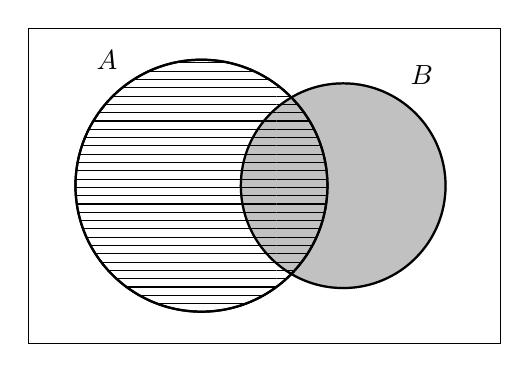
\begin{tikzpicture}
  \draw(0,0) rectangle (6,4);
  \draw(1,3.6) node{$A$};
  \draw(5,3.4) node{$B$};
  \draw[thick,fill=black!80,opacity=0.3](4,2) circle(1.3cm);
  \draw[thick,pattern=horizontal lines](2.2,2) circle(1.6cm);
  \draw[thick](2.2,2) circle(1.6cm);
  \draw[thick](4,2) circle(1.3cm);
\end{tikzpicture}
\end{center}
\caption{A Venn diagram illustrating the definition of conditional probability.
$\Prob(A \mid B)$ is the ratio of the area of the football shaped region that is both
shaded and striped ($A \intersect B$) to the area of the shaded circle ($B$).
}
\label{fig:VennConditional}
\end{figure}

%The example above indicates how we should define conditional probability 
%generally.

%\todo{Venn Diagram}

\begin{boxedText}
%\begin{definition}[Conditional Probability]
  \label{def:condProb}%
  \myindex{conditional probability|defidx}%
  Let $A$ and $B$ be two events such that $\Prob(B) \neq 0$.  
  The \textbf{conditional probability} of $A$ given $B$ is defined by
  \[
  \Prob(A \mid B) = \frac{\Prob(A \intersect B) }{ \Prob(B) }
  \; .
  \]
  If $\Prob(B) = 0$, then $\Prob(A \mid B)$ is undefined.
%  \qed
\end{boxedText}

\begin{example}
  A class of $5$th graders was asked what color should be used for the class
  T-shirt, red or purple. 
  The table below contains a summary of the students' responses:

  \begin{center}
	\medskip
	\begin{tabular}{|l||r|r|}
	  \hline
  & \multicolumn{2}{c|}{Color}\\ 
          & Red & Purple \\ \hline \hline
	Girls & $7$    & $9$ \\ \hline
	Boys  & $10$   & $8$ \\ \hline
  \end{tabular}
  \medskip
\end{center}

  \question Suppose we randomly select a student from this class.
  Let $R$ be the event that a child prefers a red T-shirt.
  Let $B$ be the event that the child is a boy, and let $G$ be 
  the event that the child is a girl.  
  Express each of the following probabilities in words and 
  determine their values:
  \begin{multicols}{3}
  \begin{itemize}
	\item
	  $\Prob(R)$,
	\item
	  $\Prob(R \mid B)$,
	\item
	  $\Prob(B \mid R)$,
	\item
	  $\Prob(R \mid G)$,
	\item
	  $\Prob(G \mid R)$,
	\item
	  $\Prob(B \mid G)$.
  \end{itemize}
  \end{multicols}

  \answer 
  The conditional probabilities can be computed in two ways.  We can use the
  formula from the definition of conditional probability directly,
  or we can consider the condition event to be a new, smaller sample space
  and read the conditional probability from the table.
  \begin{itemize}
	\item
	  $\Prob(R) = 17/34 = 1/2$ because $17$ of the $34$ kids prefer red

	  This is the probability that a randomly selected student prefers red
	\item
	  $\displaystyle \Prob(R \mid B) = \frac{10/34}{18/34} = \frac{10}{18}$ 
	  because $10$ of the $18$ boys prefer red

	  This is the probability that a randomly selected boy prefers red
	\item
	  $\displaystyle \Prob(B \mid R)= \frac{10/34}{17/34} = \frac{10}{17}$ 
	  because $10$ of the $17$ students who prefer red are boys.

	  This is the probability that a randomly selected student who
	  prefers red is a boy.
	\item
	  $\displaystyle \Prob(R \mid G) = \frac{7/34}{16/34} = \frac{7}{16}$ 
	  because $7$ of the $16$ girls prefer red

	  This is the probability that a randomly selected girl prefers red

	\item
	  $\displaystyle \Prob(G \mid R) = \frac{7/34}{17/34} = \frac{7}{17}$ 
	  because $7$ of the $17$ kids who prefer red are girls.

	  This is the probability that a randomly selected kid who prefers red
	  is a girl.

	\item
	  $\displaystyle \Prob(B \mid G) = \frac{0}{16/34} = 0 $ because none of
	  the girls are boys.

	  This is the probability that a randomly selected girl is a boy.
%	  \qedskip
  \end{itemize}
\end{example}

One important use of conditional probability is as a tool to calculate the 
probability of an intersection.

\bigskip  %improve page break

\begin{boxedText}
  \label{lem:probOfInt}
  Let $A$ and $B$ be events with non-zero probability.  Then 
  \begin{align*}
  \Prob(A \intersect B) & =  \Prob(A) \cdot \Prob(B \mid A) \\
  	& =  \Prob(B) \cdot \Prob(A \mid B)  \;.
\end{align*}

  This follows directly from the definition of conditional probability by
  a little bit of algebra and can be generalized to more than two events.
\end{boxedText}

\begin{example}
  \question
  \myindex{dice|exampleidx}%
  If you roll two standard dice, what is the probability of doubles?
  (Doubles is when the two numbers match.)

  \answer
  Let $A$ be the event that we get a number between $1$ and $6$ on the first die.
  So $\Prob(A) = 1$.  Let $B$ be the event that the second number matches
  the first.  Then the probability of doubles is 
  $\Prob(A \intersect B) = \Prob(A) \cdot \Prob(B \mid A) = 1 \cdot \frac16 = \frac16$
  since regardless of what is rolled on the first die, $1$ of the $6$ possibilities 
  for the second die will match it.
\end{example}


\bigskip % improve page break

\begin{example}
  \myindex{cards|exampleidx}%
  \question
  A $5$-card hand is dealt from a standard $52$-card deck.
  What is the probability of getting a flush (all cards the same suit)?

  \answer
  Imagine dealing the cards in order.
  Let $A_i$ be the event that the $i$th card is the same suit as all
  previous cards.
  Then 
  \begin{eqnarray*}
\evProb{flush} & = & \Prob(A_1 
  \intersect  A_2
  \intersect  A_3
  \intersect  A_4
  \intersect  A_5) \\
  & = &  \Prob(A_1) 
  	\cdot \Prob(A_2 \mid A_1)
  	\cdot \Prob(A_3 \mid A_1 \intersect A_2)
  	\cdot \Prob(A_4 \mid A_1 \intersect A_2 \intersect A_3)
	\\ & &
  	\cdot \Prob(A_5 \mid A_1 \intersect A_2 \intersect A_3 \intersect A_4) \\
	& = & 1 \cdot \frac{12}{51} \cdot \frac{11}{50} \cdot \frac{10}{49} 
	\cdot \frac{9}{48} \; 
\end{eqnarray*}
%\otherqedskip
\end{example}

\begin{example}
\newcommand*\redheart{\Large \ensuremath{{\color{red!80!white}\heartsuit}}}
\newcommand*\blueheart{\Large \ensuremath{{\color{blue!80!black}\varheartsuit}}}
	\question
	In a bowl are 4 red Valentine hearts and 2 blue Valentine hearts.  

	If you reach in
	without looking and select two of the Valentines, let $X$ be the number of blue
	Valentines.  Fill in the following probability table.

	\begin{center}
		\begin{tabular}{|l|c|c|c|}
			\hline
			value of $X$ & \qquad 0 \ \qquad & \qquad 1 \ \qquad & \qquad 2 \ \qquad  
			\\
			\hline
			probability & & & 
			\\
			\hline
		\end{tabular}
	\end{center}

	\answer
$\Prob(X=2) 
	= \Prob(\mbox{first is blue} \tand \mbox{second is blue})
	= \Prob(\mbox{first is blue}) \cdot \Prob( \mbox{second is blue} \mid \mbox{first is blue})
	= \frac26 \cdot \frac15 = \frac{2}{30}
$.
Similarly $\Prob(X=0) 
	= \Prob(\mbox{first is red} \tand \mbox{second is red})
	= \Prob(\mbox{first is red}) \cdot \Prob( \mbox{second is red} \mid \mbox{first is red})
	= \frac46 \cdot \frac35 = \frac{12}{30}
$
Finally, $\Prob(X=1) = 1 - \Prob(X=0) - \Prob(X=2) = 1 - \frac{14}{30} = \frac{16}{30}$

We can represent this using a \term{tree diagram} as well.

\begin{center}
	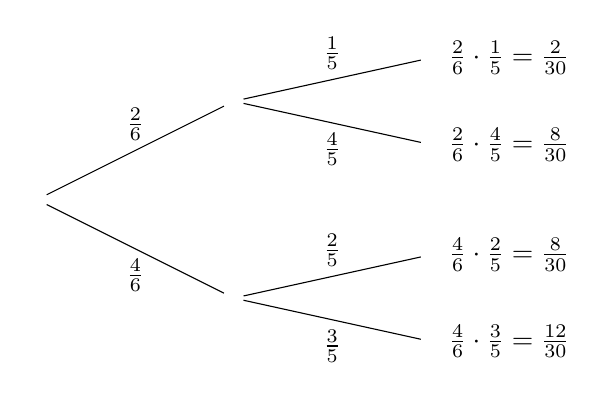
\begin{tikzpicture}
		[level 1/.style={sibling distance=25mm},
		 level 2/.style={sibling distance=11mm},
		 level distance=25mm] 
			\node {} [grow'=right]
			child {node {\blueheart} 
				child {node (bb) {\blueheart} edge from parent node[above]{$\frac15$}} 
				child {node (br) {\redheart}  edge from parent  node[below]{$\frac45$}} 
				edge from parent node[above]{$\frac26$} 
				}
			child {node {\redheart}  
				child {node (rb) {\blueheart} edge from parent  node[above]{$\frac25$}} 
				child {node (rr) {\redheart}  edge from parent  node[below]{$\frac35$}} 
				edge from parent node[below]{$\frac46$} 
			} ; 
			\node [right of=bb] {$\frac26 \cdot \frac15 = \frac{2}{30}$};
			\node [right of=br] {$\frac26 \cdot \frac45 = \frac{8}{30}$};
			\node [right of=rb] {$\frac46 \cdot \frac25 = \frac{8}{30}$};
			\node [right of=rr] {$\frac46 \cdot \frac35 = \frac{12}{30}$};
	\end{tikzpicture}
\end{center}
The edges in the tree represent conditional probabilities which we can multiply together
to the probability that all events on a particular branch happen.  The first level of branching 
represents what kind of Valentine is selected first, the second level represents the 
second selection.
	
\end{example}

\newpage

\begin{example}
  \label{example:sensitivitySpecificity}%
  \question
  Suppose a test correctly 
%  \myindex{sensitivity|exampleidx}%
%  \myindex{specificity|exampleidx}%
  \myindex{medical testing|exampleidx}%
  identifies diseased people $99$\% of the time and correctly
  identifies healthy people $98$\% of the time.  
  Furthermore assume that in a certain population,
  one person in $1000$ has the disease.  
  If a random person is tested and the test comes back positive, 
  what is the probability that the person has the disease?

  \answer
  We begin by introducing some notation.  Let $D$ be the event that
  a person has the disease.  Let $H$ be the event that the person is
  healthy.  Let $+$ be the event that the test comes back positive (meaning 
  it indicates disease -- probably a negative from the perspective 
  of the person tested).  Let $-$ be the event that the test is negative.
	\begin{itemize}
	  \item $\Prob(D) = 0.001$, so $\Prob(H) = 0.999$.

	  \item $\Prob(+ \mid D) = 0.99$, so 
	  $\Prob(- \mid D) = 0.01$.

		$\Prob(+ \mid D)$ is called the \term{sensitivity} of the test.
		(It tells how sensitive the test is to the presence of the disease.)
	  \item 
		$\Prob(-\mid H) = 0.98$, so $\Prob(+\mid H) = 0.02$.
		\medskip

	  $\Prob(- \mid H)$ is called the \term{specificity} of the test.
		\smallskip

	  \item $\!\!\!\!\!$
	  \begin{tabular}[t]{rcl}
	  $\ds \Prob(D \mid +) $
		&$\!=\!$& $\displaystyle \frac{\Prob(D \intersect +)}{\Prob(+)}$
		\\[5mm]
		&$\; = \;$& 
		$\displaystyle \frac{\Prob(D) \cdot \Prob(+ \mid D)}{\Prob(D \intersect +) 
			+ \Prob(H \intersect +)  }$
			\\[5mm]
			& $\!=\!$ & $\displaystyle 
				\frac{0.001 \cdot 0.99}{0.001 \cdot 0.99 + 0.999 \cdot 0.02}
		            \; = \;  0.0472$. 
		\end{tabular}
	  \end{itemize}
	  A tree diagram is a useful way to visualize these calculations.
\begin{center}
	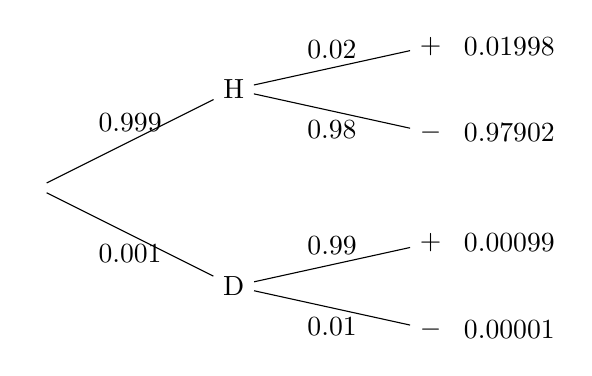
\begin{tikzpicture}
		[level 1/.style={sibling distance=25mm},
		 level 2/.style={sibling distance=11mm},
		 level distance=25mm] 
			\node {} [grow'=right]
			child {node {H} 
				child {node (bb) {$+$} edge from parent node[above]{$0.02$}} 
				child {node (br) {$-$}  edge from parent  node[below]{$0.98$}} 
				edge from parent node[above]{$0.999$} 
				}
			child {node {D}  
				child {node (rb) {$+$} edge from parent  node[above]{$0.99$}} 
				child {node (rr) {$-$}  edge from parent  node[below]{$0.01$}} 
				edge from parent node[below]{$0.001$} 
			} ; 
			\node [right of=bb] {0.01998 };
			\node [right of=br] {0.97902 };
			\node [right of=rb] {0.00099 };
			\node [right of=rr] {0.00001 };
	\end{tikzpicture}
\end{center}

	  This low probability surprises most people the first time they see it.
	  This means that if the test result of a random person comes back positive,
	  the probability that that person has the disease is less than $5$\%, 
	  even though the test is ``highly accurate''.   
	  This is one reason why we do not routinely 
	  screen an entire population for a rare disease -- such screening would 
	  produce many more false positives than true positives.

	  Of course, if a doctor orders a test, it is usually because there 
	  are some other symptoms.  This changes the \emph{a priori} probability
	  that the patient has the disease.  
%	  Exercise~\ref{prob:bayesDisease}
%	  gives you a chance to explore this further.
\end{example}

\newpage

\subsection{Independence}

\begin{boxedText}
  \label{def:independentEvents}%
  \myindex{independent events|defidx}%
  Let $A$ and $B$ be two events such that $\Prob(B) = \Prob(B \mid A)$.
  Such events are called \term{independent}.
\end{boxedText}

When events are independent, then 
$\Prob(A \tand B) = \Prob(A) \cdot \Prob(B \mid A) = \Prob(A) \cdot \Prob(B)$.
This makes probability calculations much simpler -- but it only applies
for independent events.

\begin{example}
	\question 
	What is the probability of rolling double sixes with standard 6-sided dice?

	\answer
	Let $A$ be the event that the first die is a 6 and let $B$ be the event that the 
	second die is a 6.  Since $A$ and $B$ are independent, 
	$\Prob(A \tand B) = \Prob(A) \cdot \Prob(B) = \frac16 \cdot \frac16 = \frac{1}{36}$.
\end{example}

\begin{example}
	\question What is the probability of flipping a coin five times and getting 5 heads?

	\answer  Since each coin toss is independent of the others, the probability
	of getting five heads is the product of the probabilities of each coin coming up
	heads:

	\[ 
	\Prob(\mbox{5 heads in 5 flips}) = (0.5)^5 = 0.03125 
	\]

	
\end{example}

\begin{example}
	\question
	A manufacturer claims that 99\% of its parts will still be functioning properly 
	two years after purchase.  If you purchase 10 of these parts, what is the probability
	that all 10 of them are still functioning properly two years later (assuming the
	manufacturer's claim is correct)?

	\answer
	Let $G_i$ be the event that part $i$ is still functioning properly after two years.
	We want to calculate 
	\[
	\Prob(G_1 \tand G_2 \tand \cdots \tand G_{10})\;.
	\]
	If we assume the lifetimes of the parts are independent, then 
	\[
	\Prob(G_1 \tand G_2 \tand \cdots \tand G_{10})
	=
	\underbrace{.99 \cdot .99 \cdot .99 \cdots .99 = .99^{10}}_{\mbox{10 of these}}
	= 0.9043821\;.
	\]

	The independence assumption may or may not be valid.  That depends on the manufacturing
	process.  For example, if the primary way a part goes bad is that the package 
	is dropped during shipping, then if you by a box of 10 and the first part is bad, 
	they will all be bad.  And if the box was handled carefully and never dropped, and the first part used is good, they will likely all be good.  So in
	that extreme case, the probability that all 10 are functioning properly after two years
	is 99\%.



\end{example}

\newpage
\section*{Exercises}

\begin{problem}
	Amy is a 92\% free throw shooter.  If she shoots
	100 free throws after practice, what is the probability that she
	makes at least 95 of them?  Use simulation to estimate this probability.

	(You can use \function{rflip()} to simulate shooting free throws.
	The \option{prob} argument lets you set the probability.  In this case,
	you need to set it to $0.92$.  Then think of a head as a made free throw
	and a tail as a missed free throw.)
\end{problem}

\begin{solution}
\begin{knitrout}
\definecolor{shadecolor}{rgb}{0.969, 0.969, 0.969}\color{fgcolor}\begin{kframe}
\begin{alltt}
\hlkwd{set.seed}\hlstd{(}\hlnum{123}\hlstd{)}  \hlcom{# so we get the same simulated results each time we compile.}
\hlstd{sims} \hlkwb{<-} \hlkwd{do}\hlstd{(}\hlnum{1000}\hlstd{)} \hlopt{*} \hlkwd{rflip}\hlstd{(}\hlnum{100}\hlstd{,} \hlkwc{prob} \hlstd{=} \hlnum{0.92}\hlstd{)}
\hlkwd{tally}\hlstd{(}\hlopt{~}\hlstd{heads} \hlopt{>} \hlnum{95}\hlstd{,} \hlkwc{data} \hlstd{= sims)}
\end{alltt}
\begin{verbatim}
## 
##  TRUE FALSE 
##    94   906
\end{verbatim}
\end{kframe}
\end{knitrout}
So the probability that Amy makes more than 95 shots in 100 attempts is approximately
0.094
\end{solution}

\begin{problem}
	\begin{enumerate}
		\item
	Use simulation to estimate the probability of rolling a difference of 2 when rolling
	two fair six-sided dice.
\item
	Make a histogram showing the results for all of the possible differences.
	\end{enumerate}

\end{problem}

\begin{solution}
\begin{knitrout}
\definecolor{shadecolor}{rgb}{0.969, 0.969, 0.969}\color{fgcolor}\begin{kframe}
\begin{alltt}
\hlstd{d} \hlkwb{<-} \hlstd{die1} \hlopt{-} \hlstd{die2}
\hlkwd{tally}\hlstd{(}\hlopt{~}\hlstd{d)}
\end{alltt}
\begin{verbatim}
## 
##   -5   -4   -3   -2   -1    0    1    2    3    4    5 
##  276  551  823 1100 1395 1651 1398 1159  814  545  288
\end{verbatim}
\begin{alltt}
\hlkwd{prop}\hlstd{(}\hlopt{~}\hlstd{(d} \hlopt{==} \hlnum{8}\hlstd{))}
\end{alltt}


{\ttfamily\noindent\itshape\color{messagecolor}{\#\#\ \ \ \  target level: TRUE;\ \ other levels: FALSE}}\begin{verbatim}
## TRUE 
##    0
\end{verbatim}
\begin{alltt}
\hlkwd{histogram}\hlstd{(}\hlopt{~}\hlstd{d,} \hlkwc{width} \hlstd{=} \hlnum{1}\hlstd{)}  \hlcom{# setting width is important for integer data}
\end{alltt}
\end{kframe}

{\centering \includegraphics[width=\maxwidth]{figures/fig-unnamed-chunk-51-1} 

}



\end{knitrout}
\end{solution}

\begin{problem}
	Use simulation to estimate the probability that when dealing 
	5 cards from a standard (well-shuffled) deck of 52 cards
	all five are diamonds.  

	You can simulate the deck of cards using the numbers 1 through 52 and consider the numbers
	1 through 13 to be the diamonds.  Instead of using \function{resample()}, which would allow
	you to get the same card more than once, we need to use \function{sample()}, which does not.
	(You can also use \function{deal()} which does the same thing.)
\begin{knitrout}
\definecolor{shadecolor}{rgb}{0.969, 0.969, 0.969}\color{fgcolor}\begin{kframe}
\begin{alltt}
\hlkwd{sample}\hlstd{(}\hlnum{1}\hlopt{:}\hlnum{52}\hlstd{,} \hlnum{5}\hlstd{)}
\end{alltt}
\begin{verbatim}
## [1] 19 26 36 30 21
\end{verbatim}
\begin{alltt}
\hlkwd{sample}\hlstd{(}\hlnum{1}\hlopt{:}\hlnum{52}\hlstd{,} \hlnum{5}\hlstd{)}
\end{alltt}
\begin{verbatim}
## [1] 52 10 21 28 12
\end{verbatim}
\begin{alltt}
\hlkwd{deal}\hlstd{(}\hlnum{1}\hlopt{:}\hlnum{52}\hlstd{,} \hlnum{5}\hlstd{)}
\end{alltt}
\begin{verbatim}
## [1] 19  8 52 51 18
\end{verbatim}
\begin{alltt}
\hlkwd{deal}\hlstd{(}\hlnum{1}\hlopt{:}\hlnum{52}\hlstd{,} \hlnum{5}\hlstd{)}
\end{alltt}
\begin{verbatim}
## [1] 30 23 20 51 15
\end{verbatim}
\end{kframe}
\end{knitrout}
	There is another way to make the calculation, using the function \function{sum}. \R\ can tell you how many cards are below 14 using \function{sum} because \R\ turns TRUE into 1
	and FALSE into 0 when you do a sum.
\begin{knitrout}
\definecolor{shadecolor}{rgb}{0.969, 0.969, 0.969}\color{fgcolor}\begin{kframe}
\begin{alltt}
\hlkwd{sum}\hlstd{(}\hlkwd{sample}\hlstd{(}\hlnum{1}\hlopt{:}\hlnum{52}\hlstd{,} \hlnum{5}\hlstd{)} \hlopt{<} \hlnum{14}\hlstd{)}
\end{alltt}
\begin{verbatim}
## [1] 1
\end{verbatim}
\begin{alltt}
\hlkwd{sum}\hlstd{(}\hlkwd{sample}\hlstd{(}\hlnum{1}\hlopt{:}\hlnum{52}\hlstd{,} \hlnum{5}\hlstd{)} \hlopt{<} \hlnum{14}\hlstd{)}
\end{alltt}
\begin{verbatim}
## [1] 1
\end{verbatim}
\begin{alltt}
\hlkwd{sum}\hlstd{(}\hlkwd{sample}\hlstd{(}\hlnum{1}\hlopt{:}\hlnum{52}\hlstd{,} \hlnum{5}\hlstd{)} \hlopt{<} \hlnum{14}\hlstd{)}
\end{alltt}
\begin{verbatim}
## [1] 2
\end{verbatim}
\end{kframe}
\end{knitrout}
	You can use \function{do()} to do this many times. (Three is \emph{not} many\! We just do a small number here 
	for illustration purposes.)
\begin{knitrout}
\definecolor{shadecolor}{rgb}{0.969, 0.969, 0.969}\color{fgcolor}\begin{kframe}
\begin{alltt}
\hlkwd{do}\hlstd{(}\hlnum{3}\hlstd{)} \hlopt{*} \hlkwd{sum}\hlstd{(}\hlkwd{sample}\hlstd{(}\hlnum{1}\hlopt{:}\hlnum{52}\hlstd{,} \hlnum{5}\hlstd{)} \hlopt{<} \hlnum{14}\hlstd{)}
\end{alltt}
\begin{verbatim}
##   result
## 1      0
## 2      1
## 3      1
\end{verbatim}
\end{kframe}
\end{knitrout}
\end{problem}

\begin{solution}
\begin{knitrout}
\definecolor{shadecolor}{rgb}{0.969, 0.969, 0.969}\color{fgcolor}\begin{kframe}
\begin{alltt}
\hlkwd{tally}\hlstd{(}\hlopt{~}\hlstd{result,} \hlkwd{do}\hlstd{(}\hlnum{10000}\hlstd{)} \hlopt{*} \hlkwd{sum}\hlstd{(}\hlkwd{sample}\hlstd{(}\hlnum{1}\hlopt{:}\hlnum{52}\hlstd{,} \hlnum{5}\hlstd{)} \hlopt{<} \hlnum{14}\hlstd{))}
\end{alltt}
\begin{verbatim}
## 
##    0    1    2    3    4    5 
## 2236 4094 2767  788  108    7
\end{verbatim}
\end{kframe}
\end{knitrout}
\end{solution}

\begin{problem}
Parts in a manufacturing plant go through two quality control checks before they
are shipped.  99\% of parts pass inspection A and 98\% parts pass inspection B.
0.5\% fail both inspections.  

What percentage of parts pass both inspections?
\end{problem}

\begin{solution}
	$\Prob(\mbox{fail at least one}) = \Prob(\mbox{fail A or fail B}) =
	\Prob(\mbox{fail A}) + \Prob(\mbox{fail B}) - \Prob(\mbox{fail both})
	= 0.01 + 0.02 - 0.05 = 0.025$.

	So $\Prob(\mbox{pass both}) = 1 - 0.025 = 0.975$.
\end{solution}

\begin{problem} 
	Let $X$ be the sum of the results of rolling two fair six-sided dice.
	\begin{enumerate}
		\item
			What is $\Prob(\mbox{$X$ is even and $X < 5$})$?
		\item
			What is $\Prob(\mbox{$X$ is even or $X < 5$})$? 
	\end{enumerate}
\end{problem}

\begin{solution}
	$\Prob(\mbox{$X$ is even and $X < 5$}) 
	= \Prob(X = 2 \tor X=4) = 1/36 + 3/36 = 4/36 = 0.0833333$

$\Prob(\mbox{$X$ is even or $X < 5$}) = \Prob(\mbox{$X$ is even}) + \Prob(X=3)
= 18/36 + 2/36 = 20/36 = 0.5555556$.
\end{solution}

\begin{problem}
Let $Y$ be the difference between the larger and smaller number when two fair dice 
are rolled.  (So if you roll a 2 and a 4, then the value of $Y$ is 2.)  
\begin{enumerate}
	\item 
		What is $\Prob(Y=2)$?
	\item
		What are the other possible values of $Y$?
	\item 
		Calculate the probability for each possible value of $Y$
		and put those values in a table.
\end{enumerate}
\end{problem}

\begin{solution}
	$Y = 2$ for rolls of $(3,1)$, $(4,2)$, $(5,3)$, and $(6,4)$.  Each of these 
	can also happen in the other order, so the probability is $8/36 = 2/9 = 0.2222222$.

\begin{center}
	\begin{tabular}{lrrrrrr}
		\hline
		value of $Y$ & 0 & 1 & 2 & 3 & 4 & 5 \\
		\hline
		probability & 6/36 & 10/36 & 8/36 & 6/36 & 4/36 & 2/36 \\
		\hline
	\end{tabular}
\end{center}
\begin{knitrout}
\definecolor{shadecolor}{rgb}{0.969, 0.969, 0.969}\color{fgcolor}\begin{kframe}
\begin{alltt}
\hlkwd{c}\hlstd{(}\hlnum{6}\hlstd{,} \hlnum{10}\hlstd{,} \hlnum{8}\hlstd{,} \hlnum{6}\hlstd{,} \hlnum{4}\hlstd{,} \hlnum{2}\hlstd{)}\hlopt{/}\hlnum{36}
\end{alltt}
\begin{verbatim}
## [1] 0.16666667 0.27777778 0.22222222 0.16666667 0.11111111 0.05555556
\end{verbatim}
\end{kframe}
\end{knitrout}
\end{solution}

\begin{problem}
	A device is assembled from two primary parts.  2\% of the first type of part
	are defective and 3\% of the other type of part are defective.  The device
	only functions properly if both parts are functioning properly.
	\begin{enumerate}
	\item
	What assumption do you need to make to calculate the probability
	that a device assembled in this way will function properly?
	Is it a reasonable assumption in this situation?  Explain.
	\item
	What is the probability that that a device assembled in this way will 
	function properly?
	\end{enumerate}
\end{problem}

\begin{solution}
	Assuming failure of each part is independent of failure of the other,
	the probability that both function properly is 
	$0.98 \cdot 0.97 = 0.9506$.
\end{solution}

\begin{problem}
According to the CDC, ``Compared to nonsmokers, men who smoke are about 23
times more likely to develop lung cancer and women who smoke are about 13 times
more likely.''  According to the American Lung Association: 
``In 2008, 21.1 million (18.3\%) women smoked in the United States 
compared to 24.8 million (23.1\%) men.''

\begin{enumerate}
	\item
		If you learn that a person is a smoker and no nothing else 
		about the person, what is the probability that the person is a woman?
	\item
		If you learn that a woman has been diagnosed with lung cancer,
		and you know nothing else about her, what is the probability that she is a
		smoker?
	\item
		If you learn that a man has been diagnosed with lung cancer,
		and you know nothing else about him, what is the probability that he is a
		smoker?
\end{enumerate}
\end{problem}

\begin{solution}
\begin{knitrout}
\definecolor{shadecolor}{rgb}{0.969, 0.969, 0.969}\color{fgcolor}\begin{kframe}
\begin{alltt}
\hlcom{# a)}
\hlnum{21.1}\hlopt{/}\hlstd{(}\hlnum{21.1} \hlopt{+} \hlnum{24.8}\hlstd{)}
\end{alltt}
\begin{verbatim}
## [1] 0.459695
\end{verbatim}
\end{kframe}
\end{knitrout}
Part b is the most interesting (once you can do that, you can do part c the same way).
Let $W$ be the event that someone is a woman, $S$ that they are a smoker, and $C$ that they
get cancer. Let $x = \Prob( C | W \intersect S^c)$.  Then $\Prob( C | W \intersect S ) = 13x$.

\begin{align*}
	\Prob( S | W \intersect C ) 
	& = \frac{ \Prob(S \intersect W \intersect C) }{\Prob(W \intersect C)}
	\\
	& = \frac{ \Prob(S \intersect W \intersect C) }
	{\Prob(S \intersect W \intersect C) + \Prob( S^c \intersect W \intersect C)}
\end{align*}
So we just need to compute the two probabilities in the denominator.
\begin{align*}
	\Prob(S \intersect W \intersect C)
	&= \Prob(W) \cdot \Prob(S \mid W) \cdot \Prob(C \mid W \intersect S) 
	\\
	&= \Prob(W) \cdot 0.183 \cdot 13x
	\\
	\Prob(S^c \intersect W \intersect C)
	&= \Prob(W) \cdot \Prob(S^c \mid W) \cdot \Prob(C \mid W \intersect S^c) 
	\\
	&= \Prob(W) \cdot 0.817 \cdot x
\end{align*}
After factoring out $x \cdot \Prob(W)$, the arithmetic is now easy:

\begin{knitrout}
\definecolor{shadecolor}{rgb}{0.969, 0.969, 0.969}\color{fgcolor}\begin{kframe}
\begin{alltt}
\hlcom{# b) After factoring out a constant from numerator and denominator we are left with}
\hlnum{0.183} \hlopt{*} \hlnum{13}\hlopt{/}\hlstd{(}\hlnum{0.183} \hlopt{*} \hlnum{13} \hlopt{+} \hlnum{0.817} \hlopt{*} \hlnum{1}\hlstd{)}
\end{alltt}
\begin{verbatim}
## [1] 0.744368
\end{verbatim}
\begin{alltt}
\hlcom{# c) After factoring out a constant from numerator and denominator we are left with}
\hlnum{0.231} \hlopt{*} \hlnum{23}\hlopt{/}\hlstd{(}\hlnum{0.231} \hlopt{*} \hlnum{23} \hlopt{+} \hlnum{0.769} \hlopt{*} \hlnum{1}\hlstd{)}
\end{alltt}
\begin{verbatim}
## [1] 0.8735613
\end{verbatim}
\end{kframe}
\end{knitrout}

Note: Another approach to part b is to consider the sample space to be only the women.
If you do it that way, you can avoid mentioning any probabilities involving $W$.  (In the end, 
they factor out anyway.)  Of course, you can do a similar thing for the men.
\end{solution}

\begin{problem}
A manufacturing plant has kept records that show that the number of parts produced each 
day and on the proportion of parts that are defective.

\begin{center}
\begin{tabular}{|lrrrr|}
	\hline
	& Monday & Tuesday & Wednesday & Thursday \\
	\hline
	Proportion of weekly production & 20\% & 25\% & 28\% & 27\%  
	\\
	Rate of defective parts & 2\% & 1.5\% & 1\%  & 3\% 
	\\
	\hline
\end{tabular}
\end{center}
\begin{enumerate}
	\item
		If you order a part from this company, what is the probability that it was produced
		on a Monday or a Thursday?
\item
If you order a part from this company and it is defective, 
what is the probability that it was produced on a Monday or a Thursday?
\item
	If you order a part from this company and it functions properly, 
	what is the probability that it was produced on a Monday or Thursday?
\end{enumerate}
Express your answers to 3 significant digits and avoid internal rounding.

\end{problem}

\begin{solution}
You may find a tree diagram useful here to visualize these probabilities.
\begin{knitrout}
\definecolor{shadecolor}{rgb}{0.969, 0.969, 0.969}\color{fgcolor}\begin{kframe}
\begin{alltt}
\hlcom{# part a}
\hlnum{.20} \hlopt{+} \hlnum{.27}
\end{alltt}
\begin{verbatim}
## [1] 0.47
\end{verbatim}
\begin{alltt}
\hlcom{# part b: P( Wed-Thur | defective ) = P( Wed-Thur and defective ) / P(defective)}
\hlstd{a} \hlkwb{<-} \hlnum{.20} \hlopt{*} \hlnum{.02} \hlopt{+}       \hlcom{# Monday and defective}
     \hlnum{.27} \hlopt{*} \hlnum{.03}         \hlcom{# Thursday and defective}
\hlstd{b} \hlkwb{<-} \hlnum{.25} \hlopt{*} \hlnum{.015} \hlopt{+}      \hlcom{# Tuesday and defective}
     \hlnum{.28} \hlopt{*} \hlnum{.01}         \hlcom{# Wednesday and defective }
\hlstd{a} \hlopt{/} \hlstd{(a} \hlopt{+} \hlstd{b)}
\end{alltt}
\begin{verbatim}
## [1] 0.6487936
\end{verbatim}
\begin{alltt}
\hlcom{# part c: P( Wed-Thur | good ) = P( Wed-Thur and good ) / P(good)}
\hlstd{c} \hlkwb{<-} \hlnum{.20} \hlopt{*} \hlnum{.98} \hlopt{+}       \hlcom{# Monday and good}
     \hlnum{.27} \hlopt{*} \hlnum{.97}         \hlcom{# Thursday and good}
\hlstd{d} \hlkwb{<-} \hlnum{.25} \hlopt{*} \hlnum{.985} \hlopt{+}      \hlcom{# Tuesday and good}
     \hlnum{.28} \hlopt{*} \hlnum{.99}         \hlcom{# Wednesday and good }
\hlstd{c} \hlopt{/} \hlstd{(c} \hlopt{+} \hlstd{d)}
\end{alltt}
\begin{verbatim}
## [1] 0.4666021
\end{verbatim}
\end{kframe}
\end{knitrout}
\end{solution}


\shipoutProblems

\vfill

\begin{center}
	\includegraphics[width=.4\textwidth]{images/cigarettes-cartoon}
\end{center}

\ifsolutions
\ifsolutionslocal
\newpage
\section*{Solutions}
\shipoutSolutions
\fi
\fi
 



\chapter{Densities}

\section{Density histograms, density plots, density functions}
\myindex{density|defidx}%
A histogram is a simple picture describing the ``density" of data. 
Histogram bars are tall in regions where there is more data -- i.e., where the data are 
more ``dense''.  
\begin{knitrout}
\definecolor{shadecolor}{rgb}{0.969, 0.969, 0.969}\color{fgcolor}\begin{kframe}
\begin{alltt}
\hlkwd{require}\hlstd{(alr3)}
\hlkwd{histogram}\hlstd{(}\hlopt{~}\hlstd{Duration,} \hlkwc{data} \hlstd{= oldfaith)}
\hlkwd{histogram}\hlstd{(}\hlopt{~}\hlstd{Duration,} \hlkwc{data} \hlstd{= oldfaith,} \hlkwc{type} \hlstd{=} \hlstr{"count"}\hlstd{)}
\end{alltt}
\end{kframe}

{\centering \includegraphics[width=\maxwidth]{figures/fig-histograms-count-density-1} 
\includegraphics[width=\maxwidth]{figures/fig-histograms-count-density-2} 

}



\end{knitrout}

The density scale is the same scale that is used by \function{densityplot()}, and it
is the default scale for histograms created using \function{histogram()} when
the \pkg{mosaic} package is loaded.
\begin{knitrout}
\definecolor{shadecolor}{rgb}{0.969, 0.969, 0.969}\color{fgcolor}\begin{kframe}
\begin{alltt}
\hlkwd{require}\hlstd{(alr3)}
\hlkwd{histogram}\hlstd{(}\hlopt{~}\hlstd{Duration,} \hlkwc{data} \hlstd{= oldfaith,} \hlkwc{width} \hlstd{=} \hlnum{20}\hlstd{,} \hlkwc{center} \hlstd{=} \hlnum{110}\hlstd{)}
\hlkwd{densityplot}\hlstd{(}\hlopt{~}\hlstd{Duration,} \hlkwc{data} \hlstd{= oldfaith)}
\end{alltt}
\end{kframe}

{\centering \includegraphics[width=\maxwidth]{figures/fig-histogram-density-1} 
\includegraphics[width=\maxwidth]{figures/fig-histogram-density-2} 

}



\end{knitrout}

The density scale is chosen so that the area of each rectangular bar (width times height)
is equal to the proportion of the data set represented by the rectangle. 

\begin{example}
	\question Use the histogram of Old Faithful eruption times to estimate
	the proportion of eruptions that last between 100 and 120 seconds.

	\answer
In our histogram of Old Faithful eruption durations, the bar corresponding to the 
bin from 100--120 appears to have a height of about 0.09.  That gives an area of 
0.18 and indicates that approximately 18\% of the eruptions last between 100 and 120
seconds.
\begin{knitrout}
\definecolor{shadecolor}{rgb}{0.969, 0.969, 0.969}\color{fgcolor}\begin{kframe}
\begin{alltt}
\hlkwd{tally}\hlstd{(}\hlopt{~}\hlstd{(}\hlnum{100} \hlopt{<} \hlstd{Duration} \hlopt{&} \hlstd{Duration} \hlopt{<=} \hlnum{120}\hlstd{),} \hlkwc{data} \hlstd{= oldfaith,} \hlkwc{format} \hlstd{=} \hlstr{"prop"}\hlstd{)}
\end{alltt}
\begin{verbatim}
## 
##      TRUE     FALSE 
## 0.1888889 0.8111111
\end{verbatim}
\end{kframe}
\end{knitrout}
\end{example}

The key idea behind the density scale can be expressed as 

\begin{center}
	Probability $=$ area
\end{center}
This association of area with probability means that
the total area of all the bars will always be equal to 1 if we use the density
scale.  

It also provides us with a way to describe a distribution with a mathematical function.


\begin{boxedText}
  \label{def:pdf}%
  \myindex{probability density function|defidx}%
  \myindex{density function|defidx}%
  \myindex{pdf|see{probability density function}}%
  Let $f$ be a function such that %: \reals \to \reals$ be a function such that
  \begin{enumerate}
	  \item $f(x) \ge 0$ for all $x$,
	  \item $\displaystyle \int_{-\infty}^{\infty} f(x) \; dx = 1$.
   \end{enumerate}
   Then $f$ is called a \textbf{density function} (or probability density function,
   abbreviated pdf) and describes a continuous random variable $X$ such that
   \[
   \Prob(a\le X \le b) = \int_a^b f(x) \; dx \;.
   \]
\end{boxedText}



\begin{example}
\label{ex:triangle}%
	Let $f$ be defined by
	\[
	f(x) = \begin{cases}  
		1 - |x| & x \in [-1,1] \\
		0 & \mbox{otherwise}\\
	\end{cases}
	\]
Show that $f$ is a density function.  Let $X$ be the associated random 
variable, and compute the following probabilities:
\begin{enumerate}
	\item
		$\Prob(X\le0)$
	\item
		$\Prob(X \le 1)$
	\item
		$\Prob(X \le \frac12)$
	\item
		$\Prob(-\frac12 X \le \frac12)$
\end{enumerate}

\answer
While we could set up integrals for these, it is easier to solve them using geometry.%
\footnote{\R\ cleverly turns TRUE and FALSE into 1 and 0 when you use them in arithmetic
expressions.  The definition of \code{f()} makes use of this conversion to simplify specifying
the cases.}
\begin{knitrout}
\definecolor{shadecolor}{rgb}{0.969, 0.969, 0.969}\color{fgcolor}\begin{kframe}
\begin{alltt}
\hlstd{f} \hlkwb{<-} \hlkwd{makeFun}\hlstd{((}\hlnum{1} \hlopt{-} \hlkwd{abs}\hlstd{(x))} \hlopt{*} \hlstd{(}\hlkwd{abs}\hlstd{(x)} \hlopt{<=} \hlnum{1}\hlstd{)} \hlopt{~} \hlstd{x)}
\hlkwd{plotFun}\hlstd{(}\hlkwd{f}\hlstd{(x)} \hlopt{~} \hlstd{x,} \hlkwc{x.lim} \hlstd{=} \hlkwd{c}\hlstd{(}\hlopt{-}\hlnum{1.5}\hlstd{,} \hlnum{1.5}\hlstd{))}
\end{alltt}
\end{kframe}

{\centering \includegraphics[width=\maxwidth]{figures/fig-unnamed-chunk-61-1} 

}



\end{knitrout}

The entire area under the curve can be found as the area of a triangle with base 2 and height 1.
\[
\int_{-\infty}^{\infty} f(x) \; dx 
=
\int_{-1}^1 f(x) \; dx
=
\frac 12 \cdot 2 \cdot 1 = 1
\]
This implies that $f$ is a density function.

\begin{enumerate}
	\item
$\Prob(X \le 1) 
=
\int_{-\infty}^{1} f(x) \; dx 
=
\int_{-1}^{1} f(x) \; dx = 1
$
\item
		$\Prob(X \le \frac12)
		=
\int_{-\infty}^{1/2} f(x) \; dx 
=
\int_{-1}^{1/2} f(x) \; dx = 1 - \frac12 \cdot \frac12 \cdot \frac12 = \frac78
$

\item
	$\Prob( -\frac12 \le X \le \frac 12 ) 
	=
	\int_{-1/2}^{1/2} f(x) \; dx 
	=
	1 - \frac28 = \frac34
	$
\end{enumerate}

We can also let \R\ do (numerical) integration for us.  There are two ways to do this.
The first method uses the \function{integrate()} function.
\begin{knitrout}
\definecolor{shadecolor}{rgb}{0.969, 0.969, 0.969}\color{fgcolor}\begin{kframe}
\begin{alltt}
\hlkwd{integrate}\hlstd{(f,} \hlopt{-}\hlnum{Inf}\hlstd{,} \hlnum{1}\hlstd{)}
\end{alltt}
\begin{verbatim}
## 1 with absolute error < 9.2e-05
\end{verbatim}
\begin{alltt}
\hlcom{# this will be more accurate since we aren't asking R to approximate something that we}
\hlcom{# already know is exactly 0}
\hlkwd{integrate}\hlstd{(f,} \hlopt{-}\hlnum{1}\hlstd{,} \hlnum{1}\hlstd{)}
\end{alltt}
\begin{verbatim}
## 1 with absolute error < 1.1e-14
\end{verbatim}
\begin{alltt}
\hlkwd{integrate}\hlstd{(f,} \hlopt{-}\hlnum{0.5}\hlstd{,} \hlnum{0.5}\hlstd{)}
\end{alltt}
\begin{verbatim}
## 0.75 with absolute error < 8.3e-15
\end{verbatim}
\begin{alltt}
\hlcom{# if you just want the value without the text saying how accurate the approximation is}
\hlkwd{integrate}\hlstd{(f,} \hlopt{-}\hlnum{0.5}\hlstd{,} \hlnum{0.5}\hlstd{)}\hlopt{$}\hlstd{value}
\end{alltt}
\begin{verbatim}
## [1] 0.75
\end{verbatim}
\end{kframe}
\end{knitrout}

An alternative approach uses \function{antiD()} from the \pkg{mosaic} package.
\begin{knitrout}
\definecolor{shadecolor}{rgb}{0.969, 0.969, 0.969}\color{fgcolor}\begin{kframe}
\begin{alltt}
\hlstd{F} \hlkwb{<-} \hlkwd{antiD}\hlstd{(} \hlkwd{f}\hlstd{(x)} \hlopt{~} \hlstd{x)}
\hlkwd{F}\hlstd{(}\hlnum{1}\hlstd{)} \hlopt{-} \hlkwd{F}\hlstd{(}\hlopt{-}\hlnum{1}\hlstd{)}        \hlcom{# total probability -- better be 1}
\end{alltt}
\begin{verbatim}
## [1] 1
\end{verbatim}
\begin{alltt}
\hlkwd{F}\hlstd{(}\hlnum{.5}\hlstd{)} \hlopt{-} \hlkwd{F}\hlstd{(}\hlopt{-}\hlnum{1}\hlstd{)}       \hlcom{# P( -1 <= X <= 0.5 )}
\end{alltt}
\begin{verbatim}
## [1] 0.875
\end{verbatim}
\begin{alltt}
\hlkwd{F}\hlstd{(}\hlnum{.5}\hlstd{)} \hlopt{-} \hlkwd{F}\hlstd{(}\hlopt{-}\hlnum{.5}\hlstd{)}      \hlcom{# P( -.5 <= X <= .5 )}
\end{alltt}
\begin{verbatim}
## [1] 0.75
\end{verbatim}
\end{kframe}
\end{knitrout}
\end{example}

\myindex{cumulative distribution function|defidx}%
\myindex{cdf|see{cumulative distribution function}}%
If we help \R\ choose the anti-derivative, we get a useful function called 
the \term{cumulative distribution function}, abbreviated cdf.


\begin{boxedText}
	If $X$ is a random variable, then the \term{cumulative distribution function} (cdf) for 
	$X$, often denoted $F_X$, is the function defined by
	\[
	F_X(x)  = \Prob(X \le x)
	\]
	That is, the output of the cdf reports the probability of being below a particular value.
	The derivative of the cdf is the pdf.
\end{boxedText}

\begin{example}
Continuing with our previous example, if we choose -1 as our lower endpoint,
then the anti-derivative will be the cdf.
\begin{knitrout}
\definecolor{shadecolor}{rgb}{0.969, 0.969, 0.969}\color{fgcolor}\begin{kframe}
\begin{alltt}
\hlstd{F} \hlkwb{<-} \hlkwd{antiD}\hlstd{(} \hlkwd{f}\hlstd{(x)} \hlopt{~} \hlstd{x,} \hlkwc{lower.bound} \hlstd{=} \hlopt{-}\hlnum{1}\hlstd{)}   \hlcom{# We can use -1 instead of -Inf here.}
\hlkwd{F}\hlstd{(}\hlopt{-}\hlnum{1}\hlstd{)}               \hlcom{# this should be 0 since we chose -1 as the lower bound.}
\end{alltt}
\begin{verbatim}
## [1] 0
\end{verbatim}
\begin{alltt}
\hlkwd{F}\hlstd{(}\hlnum{1}\hlstd{)}                \hlcom{# P(X <= 1); should be 1}
\end{alltt}
\begin{verbatim}
## [1] 1
\end{verbatim}
\begin{alltt}
\hlkwd{F}\hlstd{(}\hlnum{.5}\hlstd{)}               \hlcom{# P(X <= 0.5)}
\end{alltt}
\begin{verbatim}
## [1] 0.875
\end{verbatim}
\begin{alltt}
\hlkwd{F}\hlstd{(}\hlnum{.5}\hlstd{)} \hlopt{-} \hlkwd{F}\hlstd{(}\hlopt{-}\hlnum{.5}\hlstd{)}      \hlcom{# P( -0.5 <= X <= 0.5 )}
\end{alltt}
\begin{verbatim}
## [1] 0.75
\end{verbatim}
\end{kframe}
\end{knitrout}
\end{example}

\section{Working with Probability Density Funcitons}

We have already seen that we can use a pdf $f$ to calculate probabilities via integration, 
and that there is a special anti-derivative of $f$ called the cdf such that the cdf $F$
satisfies
\[
F(x) = \Prob(X \le x)
\]
This function can also be used to compute probabilities, since
\[
\Prob(a \le X \le b) = \int_a^b f(x) \; dx = F(b) - F(a)
\]
Indeed, once we learn how to get the cdf function in \R\ this will 
be our primary way to calculate probabilities in applications.

\subsection{Kernels}
\myindex{kernel|defidx}%
The \term{kernel} of a random variable is a function that is a 
constant multiple of the pdf.  The reason that these are interesting
is that any kernel can be converted into a pdf by dividing by the appropriate constant.
In particular, if 
\[ 
\int_{-\infty}^{\infty} k(x) \; dx = A \;, 
\]
then $k$ is the kernel of a random variable with pdf
\[ 
f(x) = \frac{k(x)}{A} \;.
\]

\begin{example}
\label{ex:kernel}%
	\question
	The kernel of a random variable is given by 
	\[
	k(x) = x^2 \; \boolval{ x \in [0,2] } \; .
	\]
	Determine the pdf.

	\answer First we determine the value of the integral
	\[
\int_{-\infty}^{\infty} k(x) \; dx \;. 
\]
\begin{knitrout}
\definecolor{shadecolor}{rgb}{0.969, 0.969, 0.969}\color{fgcolor}\begin{kframe}
\begin{alltt}
\hlstd{k} \hlkwb{<-} \hlkwd{makeFun}\hlstd{(x}\hlopt{^}\hlnum{2} \hlopt{*} \hlstd{(}\hlnum{0} \hlopt{<=} \hlstd{x} \hlopt{&} \hlstd{x} \hlopt{<=} \hlnum{2}\hlstd{)} \hlopt{~} \hlstd{x)}
\hlkwd{plotFun}\hlstd{(}\hlkwd{k}\hlstd{(x)} \hlopt{~} \hlstd{x,} \hlkwc{xlim} \hlstd{=} \hlkwd{c}\hlstd{(}\hlopt{-}\hlnum{1}\hlstd{,} \hlnum{3}\hlstd{))}
\hlkwd{integrate}\hlstd{(k,} \hlnum{0}\hlstd{,} \hlnum{2}\hlstd{)}
\end{alltt}
\begin{verbatim}
## 2.666667 with absolute error < 3e-14
\end{verbatim}
\begin{alltt}
\hlstd{K} \hlkwb{<-} \hlkwd{antiD}\hlstd{(}\hlkwd{k}\hlstd{(x)} \hlopt{~} \hlstd{x,} \hlkwc{lower.bound} \hlstd{=} \hlnum{0}\hlstd{)}
\hlkwd{K}\hlstd{(}\hlnum{2}\hlstd{)}
\end{alltt}
\begin{verbatim}
## [1] 2.666667
\end{verbatim}
\end{kframe}

{\centering \includegraphics[width=\maxwidth]{figures/fig-unnamed-chunk-65-1} 

}



\end{knitrout}
Since the total area is $8/3$, if $\frac{k(x)}{8/3}$ is the pdf.
\end{example}

\subsection{The mean of a continuous random variable}

The definition for the mean of a continuous random variable will be motivated 
by the calculation of a mean of some data.
\begin{example}
	\question
  Suppose a student has taken $10$ courses
  and received $5$ A's, $4$ B's, and $1$ C.  Using the traditional numerical scale where 
  an A is worth $4$, a B is worth $3$, and a C is worth $2$, what is this student's 
  GPA (grade point average)?

  \answer
  The first thing to notice is that $\frac{4 + 3 + 2}{3} = 3$ is \emph{not} correct.
  We cannot simply add up the values and divide by the number of values.  Clearly
  this student should have a GPA that is higher than $3.0$, since there were more A's than
  C's.

  Consider now a correct way to do this calculation:
  \begin{align*}
	\mbox{GPA} &= \frac{4 + 4 + 4 + 4 + 4 + 3 + 3 + 3 + 3 + 2}{10}
	\\[2mm]
	& = \frac{5\cdot 4 + 4\cdot 3 + 1 \cdot 2}{10} \\[1mm]
	& = \frac{5}{10} \cdot 4 + \frac{4}{10}\cdot 3 + \frac{1}{10} \cdot 2 \\
	& = 4 \cdot \frac{5}{10} + 3 \cdot \frac{4}{10} + 2 \cdot \frac{1}{10} \\
	& =  3.4 \;.
\end{align*}
\end{example}
The key idea here is that the mean is a \textbf{sum of values times probabilities}.  
\[
\mbox{mean} = \sum \mbox{value} \cdot \mbox{probability}
\]
When working with a continuous random variable, 
we replace the sum with an integral and replace the 
probabilities with our density function to get the following definition:

\[
\E(X) = \mu_X = \int_{-\infty}^{\infty} x f(x) \; dx
\]

If you recall doing center of mass problems you may recognize this integral as 
the first moment.
(For pdfs, we don't need to divide by the ``mass'' because the total ``mass'' is the area under the curve, which will always be 1 for a random variable).

Note: It is possible that the integral used to define the mean will fail to converge.
In that case, we say that the random variable has no mean or that the mean fails to exist.%
\footnote{Actually, we will require that $\int_{\infty}^{\infty} |x| f(x) \; dx$ converges.  
If this integral fails to converge, we will also say that the distribution has no mean.}

\begin{example}
	\question Compute the mean of our triangle distribution from Example~\ref{ex:triangle}.

	\answer We simply compute the integral from the definition.

	\begin{align*}
	\E(X) & = \int_{-1}^{1} x f(x) \; dx 
	\\
	& = \int_{-1}^{0} x (x-1) \; dx + \int_{0}^1 x ( 1-x ) \; dx 
	\\
	& = \int_{-1}^{0} x^2-x) \; dx + \int_{0}^1 x-x^2 ) \; dx  
	\\
	& = \left.\frac{x^3}{3} - \frac{x^2}{2} \right|_{-1}^0
	+ \left. \frac{x^2}{2} - \frac{x^3}{3} \right|_{0}^1
	\\
	& = \frac13 - \frac12 + \frac12 - \frac13 = 0
	\end{align*}

	This isn't surprising, by symmetry we would expect this result.

	We could also calculate this numerically in \R:
\begin{knitrout}
\definecolor{shadecolor}{rgb}{0.969, 0.969, 0.969}\color{fgcolor}\begin{kframe}
\begin{alltt}
\hlstd{f} \hlkwb{<-} \hlkwd{makeFun}\hlstd{((}\hlnum{1} \hlopt{-} \hlkwd{abs}\hlstd{(x))} \hlopt{*} \hlstd{(}\hlkwd{abs}\hlstd{(x)} \hlopt{<=} \hlnum{1}\hlstd{)} \hlopt{~} \hlstd{x)}
\hlstd{xf} \hlkwb{<-} \hlkwd{makeFun}\hlstd{(x} \hlopt{*} \hlkwd{f}\hlstd{(x)} \hlopt{~} \hlstd{x)}
\hlkwd{integrate}\hlstd{(xf,} \hlopt{-}\hlnum{1}\hlstd{,} \hlnum{1}\hlstd{)}
\end{alltt}
\begin{verbatim}
## 0 with absolute error < 3.7e-15
\end{verbatim}
\begin{alltt}
\hlstd{F} \hlkwb{<-} \hlkwd{antiD}\hlstd{(x} \hlopt{*} \hlkwd{f}\hlstd{(x)} \hlopt{~} \hlstd{x,} \hlkwc{lower.bound} \hlstd{=} \hlopt{-}\hlnum{1}\hlstd{)}
\hlkwd{F}\hlstd{(}\hlopt{-}\hlnum{1}\hlstd{)}  \hlcom{# should be 0}
\end{alltt}
\begin{verbatim}
## [1] 0
\end{verbatim}
\begin{alltt}
\hlkwd{F}\hlstd{(}\hlnum{1}\hlstd{)}
\end{alltt}
\begin{verbatim}
## [1] 0
\end{verbatim}
\end{kframe}
\end{knitrout}
\end{example}

\subsection{The variance of a continuous random variable}

Arguing similarly, we can compute the variance of a continuous random
variable using
\[
\Var(X) = \sigma^2_X = \int_{-\infty}^{\infty} (x-\mu_X)^2 f(x) \; dx
\]

Note: It is possible that the integral used to define the variance will fail to converge.
In that case, we say that the random variable has no variance or that the variance 
fails to exist.%
\footnote{Actually, we will require that $\int_{\infty}^{\infty} |x|^2 f(x) \; dx$ converges.  
If this integral fails to converge, we will say that the distribution has no variance.}

\begin{example}
	\question Compute the variance of the triangle random variable
	from the Example~\ref{ex:triangle}.
	
\answer
\begin{knitrout}
\definecolor{shadecolor}{rgb}{0.969, 0.969, 0.969}\color{fgcolor}\begin{kframe}
\begin{alltt}
\hlstd{f} \hlkwb{<-} \hlkwd{makeFun}\hlstd{((}\hlnum{1} \hlopt{-} \hlkwd{abs}\hlstd{(x))} \hlopt{*} \hlstd{(}\hlkwd{abs}\hlstd{(x)} \hlopt{<=} \hlnum{1}\hlstd{)} \hlopt{~} \hlstd{x)}
\hlstd{xxf} \hlkwb{<-} \hlkwd{makeFun}\hlstd{((x} \hlopt{-} \hlnum{0}\hlstd{)}\hlopt{^}\hlnum{2} \hlopt{*} \hlkwd{f}\hlstd{(x)} \hlopt{~} \hlstd{x)}
\hlkwd{integrate}\hlstd{(xxf,} \hlopt{-}\hlnum{1}\hlstd{,} \hlnum{1}\hlstd{)}
\end{alltt}
\begin{verbatim}
## 0.1666667 with absolute error < 1.9e-15
\end{verbatim}
\begin{alltt}
\hlstd{G} \hlkwb{<-} \hlkwd{antiD}\hlstd{((x} \hlopt{-} \hlnum{0}\hlstd{)}\hlopt{^}\hlnum{2} \hlopt{*} \hlkwd{f}\hlstd{(x)} \hlopt{~} \hlstd{x)}
\hlkwd{G}\hlstd{(}\hlnum{1}\hlstd{)} \hlopt{-} \hlkwd{G}\hlstd{(}\hlopt{-}\hlnum{1}\hlstd{)}
\end{alltt}
\begin{verbatim}
## [1] 0.1666667
\end{verbatim}
\end{kframe}
\end{knitrout}
\end{example}

Some simple algebraic manipulations of the integral above shows that
\begin{align}
\Var(X) &= \E(X^2) - \E(X)^2
\label{eqn:varshortcut}
\end{align}

\begin{problem} 
Let $f(x) = 5/4 - x^3$  on $[0,1]$.  

\begin{enumerate}
	\item
		Show that $f$ is a pdf.
	\item
			Calculate $\Prob(X \le \frac12)$.
	\item
			Calculate $\Prob(X \ge \frac12)$.
	\item
			Calculate $\Prob(X = \frac12)$.
\end{enumerate}

\end{problem}

\begin{solution}
\begin{knitrout}
\definecolor{shadecolor}{rgb}{0.969, 0.969, 0.969}\color{fgcolor}\begin{kframe}
\begin{alltt}
\hlstd{f} \hlkwb{<-} \hlkwd{makeFun}\hlstd{((}\hlnum{5}\hlopt{/}\hlnum{4} \hlopt{-} \hlstd{x}\hlopt{^}\hlnum{3}\hlstd{)} \hlopt{*} \hlstd{(}\hlkwd{abs}\hlstd{(x} \hlopt{-} \hlnum{0.5}\hlstd{)} \hlopt{<=} \hlnum{0.5}\hlstd{)} \hlopt{~} \hlstd{x)}
\hlkwd{plotFun}\hlstd{(}\hlkwd{f}\hlstd{(x)} \hlopt{~} \hlstd{x,} \hlkwc{x.lim} \hlstd{=} \hlkwd{c}\hlstd{(}\hlopt{-}\hlnum{1}\hlstd{,} \hlnum{2}\hlstd{))}  \hlcom{# quick plot to make sure things look correct.}
\hlstd{F} \hlkwb{<-} \hlkwd{antiD}\hlstd{(}\hlkwd{f}\hlstd{(x)} \hlopt{~} \hlstd{x)}
\hlcom{# part a: f(x) >=0, so we just need to check that the total area is 1}
\hlkwd{F}\hlstd{(}\hlnum{1}\hlstd{)} \hlopt{-} \hlkwd{F}\hlstd{(}\hlnum{0}\hlstd{)} \hlopt{==} \hlnum{1}
\end{alltt}
\begin{verbatim}
## [1] TRUE
\end{verbatim}
\begin{alltt}
\hlkwd{F}\hlstd{(}\hlnum{1}\hlopt{/}\hlnum{2}\hlstd{)} \hlopt{-} \hlkwd{F}\hlstd{(}\hlnum{0}\hlstd{)}  \hlcom{# part b}
\end{alltt}
\begin{verbatim}
## [1] 0.609375
\end{verbatim}
\begin{alltt}
\hlkwd{F}\hlstd{(}\hlnum{1}\hlstd{)} \hlopt{-} \hlkwd{F}\hlstd{(}\hlnum{1}\hlopt{/}\hlnum{2}\hlstd{)}  \hlcom{# part c}
\end{alltt}
\begin{verbatim}
## [1] 0.390625
\end{verbatim}
\begin{alltt}
\hlkwd{F}\hlstd{(}\hlnum{1}\hlopt{/}\hlnum{2}\hlstd{)} \hlopt{-} \hlkwd{F}\hlstd{(}\hlnum{1}\hlopt{/}\hlnum{2}\hlstd{)}  \hlcom{# part d}
\end{alltt}
\begin{verbatim}
## [1] 0
\end{verbatim}
\end{kframe}

{\centering \includegraphics[width=\maxwidth]{figures/fig-unnamed-chunk-68-1} 

}



\end{knitrout}
\end{solution}



\begin{example}
	\question Compute the mean and variance of the random variable with pdf given by
	
	\[ g(x) = \frac{3x^2}{8} \boolval{x \in [0,2]} \;. \]
	This is the pdf computed in Example~\ref{ex:kernel}.
	
\answer
\begin{knitrout}
\definecolor{shadecolor}{rgb}{0.969, 0.969, 0.969}\color{fgcolor}\begin{kframe}
\begin{alltt}
\hlstd{g} \hlkwb{<-} \hlkwd{makeFun}\hlstd{((}\hlnum{3} \hlopt{*} \hlstd{x}\hlopt{^}\hlnum{2}\hlopt{/}\hlnum{8}\hlstd{)} \hlopt{*} \hlstd{(}\hlnum{0} \hlopt{<=} \hlstd{x} \hlopt{&} \hlstd{x} \hlopt{<=} \hlnum{2}\hlstd{)} \hlopt{~} \hlstd{x)}
\hlstd{m} \hlkwb{<-} \hlkwd{antiD}\hlstd{(x} \hlopt{*} \hlkwd{g}\hlstd{(x)} \hlopt{~} \hlstd{x,} \hlkwc{lower.bound} \hlstd{=} \hlnum{0}\hlstd{)(}\hlnum{2}\hlstd{)}  \hlcom{# all in one step instead of defining F or G}
\hlstd{m}
\end{alltt}
\begin{verbatim}
## [1] 1.5
\end{verbatim}
\begin{alltt}
\hlstd{v} \hlkwb{<-} \hlkwd{antiD}\hlstd{((x} \hlopt{-} \hlstd{m)}\hlopt{^}\hlnum{2} \hlopt{*} \hlkwd{g}\hlstd{(x)} \hlopt{~} \hlstd{x,} \hlkwc{m} \hlstd{= m,} \hlkwc{lower.bound} \hlstd{=} \hlnum{0}\hlstd{)(}\hlnum{2}\hlstd{)}
\hlstd{v}
\end{alltt}
\begin{verbatim}
## [1] 0.15
\end{verbatim}
\begin{alltt}
\hlcom{# here's the alternate computation}
\hlkwd{antiD}\hlstd{(x}\hlopt{^}\hlnum{2} \hlopt{*} \hlkwd{g}\hlstd{(x)} \hlopt{~} \hlstd{x,} \hlkwc{lower.bound} \hlstd{=} \hlnum{0}\hlstd{)(}\hlnum{2}\hlstd{)} \hlopt{-} \hlstd{m}\hlopt{^}\hlnum{2}
\end{alltt}
\begin{verbatim}
## [1] 0.15
\end{verbatim}
\end{kframe}
\end{knitrout}
\end{example}

As with data, the standard deviation is the square root of the variance.

\subsection{Quantiles}

Quantiles solve equations of the form
\[
\int_{-\infty}^x f(t) \; dt = F(x) = \Prob(X \le x) = q
\]
where $q$ is known and $x$ is unknown.  So the 50th percentile (which is the 0.5-quantile
or the median) is the number such that 
\[
\Prob(X \le x) = 0.5 \;.
\]

\begin{example}
	\question What is the 25th percentile of the triangle distribution in
	Example~\ref{ex:triangle}?

	\answer
	We need to solve for $x$ in the following equation:
	\[
	0.25 = \Prob( X \le x)  \; .
	\]
	We can do this by working out the integral involved:
	\begin{align*}
	0.25 &= \int_{-1}^{x} 1 - |t| \; dt 
	\\
	 &= \int_{-1}^{x} 1 + t \; dt 
	 \\
	 &=  \left. t + t^2/2 \right|_{-1}^{x}
	 \\
	 &=   x + x^2/2 + 1 - 1^2/2  
	 \\
	 &=  x + x^2/2 + 1/2
	 \\
	 0 & =  x^2/2 + x + 1/4
	 \\
	 0 & =  2x^2 + 4x + 1
\end{align*}
So by the quadratic formula, $x = \frac12 \sqrt{2} - 1 = \ensuremath{-0.2928932}$.

We can check this by evaluating the cdf.
\begin{knitrout}
\definecolor{shadecolor}{rgb}{0.969, 0.969, 0.969}\color{fgcolor}\begin{kframe}
\begin{alltt}
\hlstd{x} \hlkwb{<-} \hlnum{1}\hlopt{/}\hlnum{2} \hlopt{*} \hlkwd{sqrt}\hlstd{(}\hlnum{2}\hlstd{)} \hlopt{-} \hlnum{1}
\hlkwd{F}\hlstd{(x)}
\end{alltt}
\begin{verbatim}
## [1] 0
\end{verbatim}
\end{kframe}
\end{knitrout}

This could also be done geometrically by solving $\frac12 y^2 = \frac14$ and letting
$x = -1 + y$.
\end{example}


\section{Some Important Families of Distributions}

\myindex{parameter}%
For now, we will consider only distributions of continuous random variables (probability density functions).  We will leave set aside discrete random variables (probability mass function) until quite a bit later in the course.

A family of distributions is a collection of distributions that share some
common features.  Typically, these are described by giving a pdf that has
one or more \term{parameters}. A parameter is simply a number that describes
(a feature of) a distribution that distinguishes between members of the family.
In this section we describe briefly
some of the important distributions and how to work with them in \R.

\subsection{Triangle Distributions}
\myindex{triangle distribution|defidx}%
\myindex{triangular distribution|see{triangle distribution}}%
The example distribution in the previous section is usually referred to as a 
triangle distribution (or triangular distribution)
because of the shape of its pdf.  There are, of course,
many triangle distributions.  A triangle distribution is specified with three
numbers: $a$, the minimum; $b$, the maximum, and $c$, the location of the peak.
A triangle distribution is symmetric if the peak is halfway between the minimum
and maximum ($c = \frac{a+b}{2}$).

When $X$ is a random variable with a triangle distribution, we will write
$X \sim \Tri(a,b,c)$.  For many of the most common
distributions, \R\ has several functions that facilitate computation with
those distributions.  The triangle distributions are not in the base \R\ 
distribution, but they can be added by requiring the \pkg{triangle} package.

For each distribution, there are four functions in \R\ that always start
with a single letter followed by a name for the distribution.  In the case 
of the triangle distributions, these functions are 

\begin{center}
\begin{tabular}{ll}
	\hline
	Function & What it does \\
	\hline
	\texttt{dtriangle(x,a,b,c)} & Computes value of the pdf at \texttt{x}
	\\
	\texttt{ptriangle(q,a,b,c)}     & Computes value of the cdf at \texttt{x}, i.e., 
	$\Prob(X \le \texttt{q})$
	\\
	\texttt{qtriangle(p,a,b,c)}     & Computes quantiles, that is a value $q$ so that 
	$\Prob(X \le \texttt{q}) = \texttt{p}$
    \\
	\texttt{rtriangle(n,a,b,c)} & Randomly samples \texttt{n} values from the 
	$\Tri(\texttt{a},\texttt{b},\texttt{c})$ distribution
	\\
	\hline
\end{tabular}
\end{center}


\begin{example}
\label{ex:triangleInR}%
	\question Let $X \sim \Tri(0,4,1)$.  Use \R\ to answer the following questions.
	\begin{enumerate}
		\item Plot the pdf for $X$.
		\item What is $\Prob(X \le 1)$?
		\item What is $\Prob(X \le 2)$?
		\item What is the median of $X$?
		\item What is the mean of $X$?
	\end{enumerate}
	
\answer
The \function{plotDist} function in the \pkg{mosaic} package allows us to 
graph the pdf for any function \R\ knows how to work with in the standard way.
For example, here is a plot of the pdf of a $\Tri(0, 4, 1)$-distribution.
\begin{knitrout}
\definecolor{shadecolor}{rgb}{0.969, 0.969, 0.969}\color{fgcolor}\begin{kframe}
\begin{alltt}
\hlkwd{require}\hlstd{(triangle)}  \hlcom{# a package that knows about triangle distributions}
\end{alltt}


{\ttfamily\noindent\itshape\color{messagecolor}{\#\# Loading required package: triangle}}\begin{alltt}
\hlkwd{plotDist}\hlstd{(}\hlstr{"triangle"}\hlstd{,} \hlkwc{params} \hlstd{=} \hlkwd{list}\hlstd{(}\hlkwc{a} \hlstd{=} \hlnum{0}\hlstd{,} \hlkwc{b} \hlstd{=} \hlnum{4}\hlstd{,} \hlkwc{c} \hlstd{=} \hlnum{1}\hlstd{))}
\end{alltt}
\end{kframe}

{\centering \includegraphics[width=\maxwidth]{figures/fig-unnamed-chunk-71-1} 

}



\end{knitrout}
Here is the \R\ code to answer the remaining questions.
\begin{knitrout}
\definecolor{shadecolor}{rgb}{0.969, 0.969, 0.969}\color{fgcolor}\begin{kframe}
\begin{alltt}
\hlkwd{ptriangle}\hlstd{(}\hlnum{1}\hlstd{,} \hlnum{0}\hlstd{,} \hlnum{4}\hlstd{,} \hlnum{1}\hlstd{)}  \hlcom{# P(X <= 4); notice that his is NOT 1/2}
\end{alltt}
\begin{verbatim}
## [1] 0.25
\end{verbatim}
\begin{alltt}
\hlkwd{ptriangle}\hlstd{(}\hlnum{2}\hlstd{,} \hlnum{0}\hlstd{,} \hlnum{4}\hlstd{,} \hlnum{1}\hlstd{)}  \hlcom{# P(X <= 4); also NOT 1/2}
\end{alltt}
\begin{verbatim}
## [1] 0.6666667
\end{verbatim}
\begin{alltt}
\hlkwd{qtriangle}\hlstd{(}\hlnum{0.5}\hlstd{,} \hlnum{0}\hlstd{,} \hlnum{4}\hlstd{,} \hlnum{1}\hlstd{)}  \hlcom{# median is the 0.5-quantile}
\end{alltt}
\begin{verbatim}
## [1] 1.55051
\end{verbatim}
\begin{alltt}
\hlstd{T} \hlkwb{<-} \hlkwd{antiD}\hlstd{(x} \hlopt{*} \hlkwd{dtriangle}\hlstd{(x,} \hlnum{0}\hlstd{,} \hlnum{4}\hlstd{,} \hlnum{1}\hlstd{)} \hlopt{~} \hlstd{x,} \hlkwc{lower.bound} \hlstd{=} \hlnum{0}\hlstd{)}
\hlkwd{T}\hlstd{(}\hlnum{4}\hlstd{)}  \hlcom{# mean of X}
\end{alltt}
\begin{verbatim}
## [1] 1.666667
\end{verbatim}
\begin{alltt}
\hlkwd{integrate}\hlstd{(}\hlkwd{makeFun}\hlstd{(x} \hlopt{*} \hlkwd{dtriangle}\hlstd{(x,} \hlnum{0}\hlstd{,} \hlnum{4}\hlstd{,} \hlnum{1}\hlstd{)} \hlopt{~} \hlstd{x),} \hlnum{0}\hlstd{,} \hlnum{4}\hlstd{)}
\end{alltt}
\begin{verbatim}
## 1.666667 with absolute error < 1.9e-14
\end{verbatim}
\end{kframe}
\end{knitrout}
\end{example}



\begin{problem}
	Repeat parts (2) -- (4) of Example~\ref{ex:triangleInR} using geometry 
	rather than \R.

\end{problem}

\begin{solution}
	\begin{itemize}
		\item
			$\Prob(X \le 1) = \frac 12 \cdot 1 \cdot \frac12 = \frac 14$
		\item
			$\Prob(X \le 2) = 1 - \Prob(X \ge 2) =  1 - \frac12 \cdot 2 \cdot \frac13 
			= 1 - \frac 13 = \frac23$.
		\item
			The median $m$ is a number between 1 and 2 and satisfies
			$\frac 12 = \Prob(X \ge m) = \frac12 (4-m) \frac{4-m}{6}$.  
			Solving for $m$ we get $m = 4 - \sqrt{6} = 1.5505103$.
	\end{itemize}
\end{solution}

\begin{problem}
	Let $\displaystyle k(x) = (1 - x^2) \cdot \boolval{ x \in [-1,1] } = 
	\begin{cases}
		1-x^2 & x \in [-1,1] \\ 
		0 & \mbox{otherwise} 
	\end{cases}$ be the kernel of a continuous distribution.
	\begin{enumerate}
		\item
			Determine the pdf for this distribution.
		\item
			Compute the mean and variance for this distribution
	\end{enumerate}
\end{problem}

\begin{solution}
	The integrals are easy enough to do by hand, but here is the \R\ code 
	to compute them.
\begin{knitrout}
\definecolor{shadecolor}{rgb}{0.969, 0.969, 0.969}\color{fgcolor}\begin{kframe}
\begin{alltt}
\hlstd{k} \hlkwb{<-} \hlkwd{makeFun}\hlstd{(} \hlnum{1} \hlopt{-} \hlstd{x}\hlopt{^}\hlnum{2} \hlopt{~} \hlstd{x )}
\hlstd{K} \hlkwb{<-} \hlkwd{antiD}\hlstd{(} \hlkwd{k}\hlstd{(x)} \hlopt{~} \hlstd{x )}
\hlstd{area} \hlkwb{<-} \hlkwd{K}\hlstd{(}\hlnum{1}\hlstd{)} \hlopt{-} \hlkwd{K}\hlstd{(}\hlopt{-}\hlnum{1}\hlstd{); area}
\end{alltt}
\begin{verbatim}
## [1] 1.333333
\end{verbatim}
\begin{alltt}
\hlstd{f} \hlkwb{<-} \hlkwd{makeFun}\hlstd{( (}\hlnum{1} \hlopt{-} \hlstd{x}\hlopt{^}\hlnum{2}\hlstd{)}\hlopt{/}\hlstd{A} \hlopt{~} \hlstd{x,} \hlkwc{A}\hlstd{=area )}
\hlstd{F} \hlkwb{<-} \hlkwd{antiD}\hlstd{(}\hlkwd{f}\hlstd{(x)} \hlopt{~} \hlstd{x)}
\hlkwd{F}\hlstd{(}\hlnum{1}\hlstd{)} \hlopt{-} \hlkwd{F}\hlstd{(}\hlopt{-}\hlnum{1}\hlstd{)}    \hlcom{# this should be 1 if we have done things right}
\end{alltt}
\begin{verbatim}
## [1] 1
\end{verbatim}
\begin{alltt}
\hlstd{G} \hlkwb{<-} \hlkwd{antiD}\hlstd{( x} \hlopt{*} \hlkwd{f}\hlstd{(x)} \hlopt{~} \hlstd{x )}
\hlstd{H} \hlkwb{<-} \hlkwd{antiD}\hlstd{( x}\hlopt{^}\hlnum{2} \hlopt{*} \hlkwd{f}\hlstd{(x)} \hlopt{~} \hlstd{x )}
\hlstd{m} \hlkwb{<-} \hlkwd{G}\hlstd{(}\hlnum{1}\hlstd{)} \hlopt{-} \hlkwd{G}\hlstd{(}\hlopt{-}\hlnum{1}\hlstd{); m}               \hlcom{# E(X)}
\end{alltt}
\begin{verbatim}
## [1] 0
\end{verbatim}
\begin{alltt}
\hlkwd{H}\hlstd{(}\hlnum{1}\hlstd{)} \hlopt{-} \hlkwd{H}\hlstd{(}\hlopt{-}\hlnum{1}\hlstd{)}                       \hlcom{# E(X^2)}
\end{alltt}
\begin{verbatim}
## [1] 0.2
\end{verbatim}
\begin{alltt}
\hlkwd{H}\hlstd{(}\hlnum{1}\hlstd{)} \hlopt{-} \hlkwd{H}\hlstd{(}\hlopt{-}\hlnum{1}\hlstd{)} \hlopt{-} \hlstd{m}\hlopt{^}\hlnum{2}                 \hlcom{# Var(X)}
\end{alltt}
\begin{verbatim}
## [1] 0.2
\end{verbatim}
\end{kframe}
\end{knitrout}
\end{solution}

\begin{problem}
	Let $Y \sim \Tri(0,10,4)$.  Compute $\E(Y)$ and the median of $Y$.
\end{problem}
\begin{solution}
\begin{knitrout}
\definecolor{shadecolor}{rgb}{0.969, 0.969, 0.969}\color{fgcolor}\begin{kframe}
\begin{alltt}
\hlcom{# mean:}
\hlstd{m} \hlkwb{<-} \hlkwd{antiD}\hlstd{(x} \hlopt{*} \hlkwd{dtriangle}\hlstd{(x,} \hlnum{0}\hlstd{,} \hlnum{10}\hlstd{,} \hlnum{4}\hlstd{)} \hlopt{~} \hlstd{x,} \hlkwc{lower.bound} \hlstd{=} \hlnum{0}\hlstd{)(}\hlnum{10}\hlstd{)}
\hlstd{m}
\end{alltt}
\begin{verbatim}
## [1] 4.666667
\end{verbatim}
\begin{alltt}
\hlcom{# variance:}
\hlkwd{antiD}\hlstd{(x}\hlopt{^}\hlnum{2} \hlopt{*} \hlkwd{dtriangle}\hlstd{(x,} \hlnum{0}\hlstd{,} \hlnum{10}\hlstd{,} \hlnum{4}\hlstd{)} \hlopt{~} \hlstd{x,} \hlkwc{lower.bound} \hlstd{=} \hlnum{0}\hlstd{)(}\hlnum{10}\hlstd{)} \hlopt{-} \hlstd{m}\hlopt{^}\hlnum{2}
\end{alltt}
\begin{verbatim}
## [1] 4.222222
\end{verbatim}
\begin{alltt}
\hlcom{# median}
\hlkwd{qtriangle}\hlstd{(}\hlnum{0.5}\hlstd{,} \hlnum{0}\hlstd{,} \hlnum{10}\hlstd{,} \hlnum{4}\hlstd{)}
\end{alltt}
\begin{verbatim}
## [1] 4.522774
\end{verbatim}
\end{kframe}
\end{knitrout}
\end{solution}

\subsection{Uniform Distributions}
\myindex{uniform distribution|defidx}%

A uniform distribution is a described by a constant function over some interval.  Its 
shape is a rectangle.  This makes it particularly easy to calculate probabilities 
for a uniform distribution.  Despite its simplicity, the family of uniform distributions
has many applications.

We will let $X \sim \Unif(a,b)$ denote that $X$ is a uniform random variable on 
the interval from $a$ to $b$. 
In \R\, the parameters $a$ and $b$ are given more meaningful names: \code{min} and \code{max}.
We can use the following code to graph the $\Unif(1,4)$ distribution.

\begin{knitrout}
\definecolor{shadecolor}{rgb}{0.969, 0.969, 0.969}\color{fgcolor}\begin{kframe}
\begin{alltt}
\hlkwd{plotDist}\hlstd{(}\hlstr{"unif"}\hlstd{,} \hlkwc{params} \hlstd{=} \hlkwd{list}\hlstd{(}\hlkwc{min} \hlstd{=} \hlnum{1}\hlstd{,} \hlkwc{max} \hlstd{=} \hlnum{4}\hlstd{),} \hlkwc{xlim} \hlstd{=} \hlkwd{c}\hlstd{(}\hlnum{0}\hlstd{,} \hlnum{5}\hlstd{))}  \hlcom{# using parameter names}
\hlkwd{plotDist}\hlstd{(}\hlstr{"unif"}\hlstd{,} \hlkwc{params} \hlstd{=} \hlkwd{list}\hlstd{(}\hlnum{1}\hlstd{,} \hlnum{4}\hlstd{),} \hlkwc{xlim} \hlstd{=} \hlkwd{c}\hlstd{(}\hlnum{0}\hlstd{,} \hlnum{5}\hlstd{))}  \hlcom{# without names}
\end{alltt}
\end{kframe}

{\centering \includegraphics[width=\maxwidth]{figures/fig-unnamed-chunk-75-1} 
\includegraphics[width=\maxwidth]{figures/fig-unnamed-chunk-75-2} 

}



\end{knitrout}
Notice that the width of the non-zero portion of the pdf is 3, so the height must be $1/3$.

Probabilities involving uniform distributions are easily calculated using simple geometry,
but \R\ also provides several functions for working with uniform probability distributions.

\begin{center}
\begin{tabular}{ll}
	\hline
	Function & What it does \\
	\hline
	\texttt{dunif(x,min,max)} & Computes value of the pdf at \texttt{x}
	\\
	\texttt{punif(x,min,max)} & Computes value of the cdf at \texttt{x}, i.e., 
	$\Prob(X \le \texttt{x})$
	\\
	\texttt{qunif(p,min,max)} & Computes quantiles, that is a value of $x$ so that 
								$\Prob(X \le x) = \texttt{q}$
    \\
	\texttt{runif(n,min,max)} & Randomly samples \texttt{n} values from the 
								$\Unif(\texttt{min}, \texttt{max})$ distribution
	\\
	\hline
\end{tabular}
\end{center}

Notice the pattern to these names.  They start with the same letters as 
the functions for the triangle distributions, but replace \texttt{triangle}
with \texttt{unif}.  \emph{There are similar functions for all of the distributions
in this chapter.}

\begin{example}
	\question
	Let $X \sim \Unif(1,4)$.  Use \R\ to calculate the following values and 
	check the values using geometry:
	\begin{enumerate}
		\item $\Prob(X \le 2)$
		\item the 80th percentile of the distribution
	\end{enumerate}

	\answer
\begin{knitrout}
\definecolor{shadecolor}{rgb}{0.969, 0.969, 0.969}\color{fgcolor}\begin{kframe}
\begin{alltt}
\hlkwd{punif}\hlstd{(}\hlnum{2}\hlstd{,} \hlnum{1}\hlstd{,} \hlnum{4}\hlstd{)}  \hlcom{# P(X <= 2 )}
\end{alltt}
\begin{verbatim}
## [1] 0.3333333
\end{verbatim}
\begin{alltt}
\hlstd{(}\hlnum{2} \hlopt{-} \hlnum{1}\hlstd{)} \hlopt{*} \hlnum{1}\hlopt{/}\hlnum{3}  \hlcom{# P(X <= 2 ) using area}
\end{alltt}
\begin{verbatim}
## [1] 0.3333333
\end{verbatim}
\begin{alltt}
\hlkwd{qunif}\hlstd{(}\hlnum{0.8}\hlstd{,} \hlnum{1}\hlstd{,} \hlnum{4}\hlstd{)}  \hlcom{# 80th percentile}
\end{alltt}
\begin{verbatim}
## [1] 3.4
\end{verbatim}
\end{kframe}
\end{knitrout}
We could also get the 80th percentile by solving the equation $\frac13 (x-1) = 0.8$
From this we get $\frac{x}{3} = 0.8 + 1/3$, so $x = 3 ( 0.8 + 1/3) = 2.4 + 1 = 3.4$.
\end{example}

\begin{problem}
	Let $W \sim \Unif(0,10)$.  Compute $\E(W)$ and $\Var(W)$.
\end{problem}

\begin{solution}
\begin{knitrout}
\definecolor{shadecolor}{rgb}{0.969, 0.969, 0.969}\color{fgcolor}\begin{kframe}
\begin{alltt}
\hlcom{# mean:}
\hlstd{m} \hlkwb{<-} \hlkwd{antiD}\hlstd{(x} \hlopt{*} \hlkwd{dunif}\hlstd{(x,} \hlnum{0}\hlstd{,} \hlnum{10}\hlstd{)} \hlopt{~} \hlstd{x,} \hlkwc{lower.bound} \hlstd{=} \hlnum{0}\hlstd{)(}\hlnum{10}\hlstd{)}
\hlstd{m}
\end{alltt}
\begin{verbatim}
## [1] 5
\end{verbatim}
\begin{alltt}
\hlcom{# variance:}
\hlkwd{antiD}\hlstd{(x}\hlopt{^}\hlnum{2} \hlopt{*} \hlkwd{dunif}\hlstd{(x,} \hlnum{0}\hlstd{,} \hlnum{10}\hlstd{)} \hlopt{~} \hlstd{x,} \hlkwc{lower.bound} \hlstd{=} \hlnum{0}\hlstd{)(}\hlnum{10}\hlstd{)} \hlopt{-} \hlstd{m}\hlopt{^}\hlnum{2}
\end{alltt}
\begin{verbatim}
## [1] 8.333333
\end{verbatim}
\end{kframe}
\end{knitrout}
\end{solution}


\subsection{Exponential Distributions}
\myindex{exponential distribution|defidx}%

The exponential distributions are useful for modeling the time until some ``event'' 
occurs.  The model is based on the assumptions that 
\begin{enumerate}
	\item
		The probability of an event occurring in any small interval of time 
		is proportional to the length of the time interval.  The constant
		of proportionality is the rate parameter, usually denoted by $\lambda$.
	\item
		The probabilities of events occurring in two small non-overlapping intervals
		are independent.
\end{enumerate}

\begin{examples}
	Here are some situations that might be well modeled by an exponential distribution:
	\begin{enumerate}
\item
	The time until the next radioactive decay event is detected on a Geiger counter 

\item
	The time until a space satellite is struck by a meteor (or some other space junk) 
	and disabled.

	The model would be good if (over some time span of interest) the chances of getting
	struck are always the same.  It would not be such a good model if the satellite moves
	through time periods of relatively higher and then relatively lower chances of being
	struck (perhaps because we pass through regions of more or less space debris at 
	different times of the year.)

\item
	The lifetime of some manufactured device.

	This is a pretty simple model (we'll learn better ones later) and most often is \emph{too} simple to describe the interesting features of the lifetime of a device.  In this model, failure is due to some external thing ``happening to" the device; the 
	device itself does not wear (or improve) over time.
	\end{enumerate}
\end{examples}

We will let $X \sim \Exp(\lambda)$ denote that $X$ has an exponential distribution
with rate parameter $\lambda$.   
The kernel of such a distribution is 
\[
k(x; \lambda) = e^{-\lambda x} \; \boolval{x \ge 0}
\]
Notice that the function describing this distribution is defined only for x-values that are real numbers greater than or equal to zero (in mathematical notation, the interval $[0, \infty)$.) This interval is sometimes called the ``support" of the distribution.  When using probability distributions to model data, it's important to think about whether the support of the distribution matches well with the range of possible values observed in the data.

The exponential distribution function is a pretty easy function to integrate, but \R\ provides the now familiar
functions to make things even easier.

\begin{center}
\begin{tabular}{ll}
	\hline
	Function & What it does \\
	\hline
	\texttt{dexp(x,rate)} & Computes value of the pdf at \texttt{x}
	\\
	\texttt{pexp(q,rate)}     & Computes value of the cdf at \texttt{x}, i.e., 
	$\Prob(X \le \texttt{q})$
	\\
	\texttt{qexp(p,rate)}     & Computes quantiles, that is a value $q$ so that 
	$\Prob(X \le \texttt{q}) = \texttt{p}$
    \\
	\texttt{rexp(n,rate)} & Randomly samples \texttt{n} values from the 
	$\Exp(\lambda)$ distribution
	\\
	\hline
\end{tabular}
\end{center}

\iffalse
\begin{boxedText}
	We will write $X \sim \Exp(\lambda)$ to indicate that the random variable $X$ has 
	an exponential distribution with rate parameter $\lambda$.
	\begin{center}
		\begin{tabular}{lll}
			\hline 
			parameter & $\lambda$ & \texttt{rate}
			\\
			kernel & $e^{-\lambda x}$
			\\
			pdf & $f(x; \lambda) = \lambda e^{-\lambda x} \boolval{x\ge 0}$ 
			& \texttt{dexp(x,rate)}
			\\
%			mean & $\frac{1}{\lambda}$
%			\\
%			variance & $\frac{1}{\lambda^2}$
%			\\ 
%			\hline
		\end{tabular}
	\end{center}
\end{boxedText}
\fi


\begin{knitrout}
\definecolor{shadecolor}{rgb}{0.969, 0.969, 0.969}\color{fgcolor}\begin{kframe}
\begin{alltt}
\hlkwd{plotDist}\hlstd{(}\hlstr{"exp"}\hlstd{,} \hlkwc{params} \hlstd{=} \hlkwd{list}\hlstd{(}\hlkwc{rate} \hlstd{=} \hlnum{4}\hlstd{))}
\end{alltt}
\end{kframe}

{\centering \includegraphics[width=\maxwidth]{figures/fig-plotDist-eponential-1} 

}



\end{knitrout}

\begin{problem}
	\begin{enumerate}
		\item Let $X \sim \Exp(4)$.  Use \R\ to compute $\E(X)$.
		\item Let $X \sim \Exp(10)$.  Use \R\ to compute $\E(X)$.
		\item Let $X \sim \Exp(1/5)$.  Use \R\ to compute $\E(X)$.
		\item What pattern do you notice.  Explain in terms of 
			the definition of the exponential distribution why this
			makes sense.
	\end{enumerate}
\end{problem}

\begin{solution}
\begin{knitrout}
\definecolor{shadecolor}{rgb}{0.969, 0.969, 0.969}\color{fgcolor}\begin{kframe}
\begin{alltt}
\hlkwd{antiD}\hlstd{(x} \hlopt{*} \hlkwd{dexp}\hlstd{(x,} \hlnum{4}\hlstd{)} \hlopt{~} \hlstd{x,} \hlkwc{lower.bound} \hlstd{=} \hlnum{0}\hlstd{)(}\hlnum{Inf}\hlstd{)}
\end{alltt}
\begin{verbatim}
## [1] 0.25
\end{verbatim}
\begin{alltt}
\hlkwd{antiD}\hlstd{(x} \hlopt{*} \hlkwd{dexp}\hlstd{(x,} \hlnum{10}\hlstd{)} \hlopt{~} \hlstd{x,} \hlkwc{lower.bound} \hlstd{=} \hlnum{0}\hlstd{)(}\hlnum{Inf}\hlstd{)}
\end{alltt}
\begin{verbatim}
## [1] 0.1
\end{verbatim}
\begin{alltt}
\hlkwd{antiD}\hlstd{(x} \hlopt{*} \hlkwd{dexp}\hlstd{(x,} \hlnum{1}\hlopt{/}\hlnum{5}\hlstd{)} \hlopt{~} \hlstd{x,} \hlkwc{lower.bound} \hlstd{=} \hlnum{0}\hlstd{)(}\hlnum{Inf}\hlstd{)}
\end{alltt}
\begin{verbatim}
## [1] 5
\end{verbatim}
\end{kframe}
\end{knitrout}
	It appears that the mean of an $\Exp(\lambda)$-distribution is $1/\lambda$.  This
	makes sense.  If events have at a rate of $30$ per hour, we would expect to wait
	$1/30$ of an hour (on average) for the first event to happen.
\end{solution}


%\newpage
\subsection{Gamma and Weibull Distributions}
\myindex{Gamma distribution|defidx}%
\myindex{Weibull distribution|defidx}%

The Gamma and Weibull familities of distributions are generalizations of the exponential
distribution.  Each family has two parameters, a rate parameter as in 
the exponential distribution, and an additional parameter called the shape 
parameter (denoted by $\alpha$ below).  The reciprocal of the rate parameter
is called the scale parameter.  For the Gamma distribution, \R\ lets us use
either rate or scale (and the default is rate).  For the Weibull, we must use the 
scale.

\begin{center}
	\begin{tabular}{ll}
		\hline
		distribution & kernel
		\\
		\hline
		$\Gamm(\alpha, \lambda)$ & $ k(x) = x^{\alpha-1} e^{-\lambda x} \; \boolval{x \ge 0}$
		\\
		$\Weibull(\alpha, \lambda)$ & $ k(x) = x^{\alpha-1} e^{-\lambda x^{\alpha}} \; \boolval{x \ge 0}$
		\\
		\hline
	\end{tabular}
\end{center}
Both families of distributions are supported on the interval $[0, \infty)$.)
For the most part, we won't use these formulas in calculations, 
preferring to let \R\ do the work for us. However, notice that each
of these distributions has a pdf that allows for relatively simple integration.  For the 
Gamma distributions, we need to use integration by parts ($\alpha - 1$ times).  For 
the Weibull distributions we can use a substitution: $u = x^{\alpha}$.
In each case, when $\alpha=1$ we get an exponential distribution.

The now familiar functions are available for each of these distributions.
\begin{center}
\begin{tabular}{ll}
	\hline
	Function & What it does \\
	\hline
	\texttt{dgamma(x, shape, rate, scale=1/rate)} & Computes value of the pdf at \texttt{x}
	\\
	\texttt{pgamma(q, shape, rate, scale=1/rate)} 
		& Computes value of the cdf at \texttt{x}, i.e., 
	$\Prob(X \le \texttt{q})$
	\\
	\texttt{qgamma(p, shape, rate, scale=1/rate)} 
		& Computes quantiles, that is a value $q$ so that 
	$\Prob(X \le \texttt{q}) = \texttt{p}$
    \\
	\texttt{rgamma(n, shape, rate, scale=1/rate)} & Randomly samples \texttt{n} values from a
	Gamma distribution.
	\\
	\hline
	\texttt{dweibull(x, shape, scale=1/rate)} & Computes value of the pdf at \texttt{x}
	\\
	\texttt{pweibull(q, shape, scale)} 
		& Computes value of the cdf at \texttt{x}, i.e., 
	$\Prob(X \le \texttt{q})$
	\\
	\texttt{qweibull(p, shape, scale)} 
		& Computes quantiles, that is a value $q$ so that 
	$\Prob(X \le \texttt{q}) = \texttt{p}$
    \\
	\texttt{rweibull(n,shape,scale)} & Randomly samples \texttt{n} values from a
	Weibull distribution.
	\\
	\hline
\end{tabular}
\end{center}

Like the exponential distributions, these distributions are skewed and only take 
on positive values.  
These distributions arise in many applications, including as more general models 
for lifetime.  As the pictures below indicate, the shape and scale parameters
are aptly named.

\begin{knitrout}
\definecolor{shadecolor}{rgb}{0.969, 0.969, 0.969}\color{fgcolor}\begin{kframe}
\begin{alltt}
\hlkwd{plotDist}\hlstd{(}\hlstr{"gamma"}\hlstd{,} \hlkwc{params} \hlstd{=} \hlkwd{list}\hlstd{(}\hlkwc{shape} \hlstd{=} \hlnum{2}\hlstd{,} \hlkwc{rate} \hlstd{=} \hlnum{1}\hlstd{),} \hlkwc{main} \hlstd{=} \hlstr{"Gamma(2,1)"}\hlstd{)}
\hlkwd{plotDist}\hlstd{(}\hlstr{"gamma"}\hlstd{,} \hlkwc{params} \hlstd{=} \hlkwd{list}\hlstd{(}\hlkwc{shape} \hlstd{=} \hlnum{5}\hlstd{,} \hlkwc{rate} \hlstd{=} \hlnum{1}\hlstd{),} \hlkwc{main} \hlstd{=} \hlstr{"Gamma(5,1)"}\hlstd{)}
\hlkwd{plotDist}\hlstd{(}\hlstr{"gamma"}\hlstd{,} \hlkwc{params} \hlstd{=} \hlkwd{list}\hlstd{(}\hlkwc{shape} \hlstd{=} \hlnum{2}\hlstd{,} \hlkwc{scale} \hlstd{=} \hlnum{10}\hlstd{),} \hlkwc{main} \hlstd{=} \hlstr{"Gamma(5,10)"}\hlstd{)}
\hlkwd{plotDist}\hlstd{(}\hlstr{"gamma"}\hlstd{,} \hlkwc{params} \hlstd{=} \hlkwd{list}\hlstd{(}\hlkwc{shape} \hlstd{=} \hlnum{5}\hlstd{,} \hlkwc{scale} \hlstd{=} \hlnum{10}\hlstd{),} \hlkwc{main} \hlstd{=} \hlstr{"Gamma(5,10)"}\hlstd{)}
\end{alltt}
\end{kframe}

{\centering \includegraphics[width=\maxwidth]{figures/fig-unnamed-chunk-79-1} 
\includegraphics[width=\maxwidth]{figures/fig-unnamed-chunk-79-2} 
\includegraphics[width=\maxwidth]{figures/fig-unnamed-chunk-79-3} 
\includegraphics[width=\maxwidth]{figures/fig-unnamed-chunk-79-4} 

}



\end{knitrout}

\begin{knitrout}
\definecolor{shadecolor}{rgb}{0.969, 0.969, 0.969}\color{fgcolor}\begin{kframe}
\begin{alltt}
\hlkwd{plotDist}\hlstd{(}\hlstr{"weibull"}\hlstd{,} \hlkwc{params} \hlstd{=} \hlkwd{list}\hlstd{(}\hlkwc{shape} \hlstd{=} \hlnum{2}\hlstd{,} \hlkwc{scale} \hlstd{=} \hlnum{1}\hlstd{),} \hlkwc{main} \hlstd{=} \hlstr{"Weibull(2,1)"}\hlstd{)}
\hlkwd{plotDist}\hlstd{(}\hlstr{"weibull"}\hlstd{,} \hlkwc{params} \hlstd{=} \hlkwd{list}\hlstd{(}\hlkwc{shape} \hlstd{=} \hlnum{5}\hlstd{,} \hlkwc{scale} \hlstd{=} \hlnum{1}\hlstd{),} \hlkwc{main} \hlstd{=} \hlstr{"Weibull(5,1)"}\hlstd{)}
\hlkwd{plotDist}\hlstd{(}\hlstr{"weibull"}\hlstd{,} \hlkwc{params} \hlstd{=} \hlkwd{list}\hlstd{(}\hlkwc{shape} \hlstd{=} \hlnum{2}\hlstd{,} \hlkwc{scale} \hlstd{=} \hlnum{10}\hlstd{),} \hlkwc{main} \hlstd{=} \hlstr{"Weibull(2,10)"}\hlstd{)}
\hlkwd{plotDist}\hlstd{(}\hlstr{"weibull"}\hlstd{,} \hlkwc{params} \hlstd{=} \hlkwd{list}\hlstd{(}\hlkwc{shape} \hlstd{=} \hlnum{5}\hlstd{,} \hlkwc{scale} \hlstd{=} \hlnum{10}\hlstd{),} \hlkwc{main} \hlstd{=} \hlstr{"Weibull(5,10)"}\hlstd{)}
\end{alltt}
\end{kframe}

{\centering \includegraphics[width=\maxwidth]{figures/fig-unnamed-chunk-80-1} 
\includegraphics[width=\maxwidth]{figures/fig-unnamed-chunk-80-2} 
\includegraphics[width=\maxwidth]{figures/fig-unnamed-chunk-80-3} 
\includegraphics[width=\maxwidth]{figures/fig-unnamed-chunk-80-4} 

}



\end{knitrout}

\subsection{Normal Distributions}
\myindex{normal distribution|defidx}%

We come now to the most famous family of distributions -- the normal
distributions (also called Gaussian distributions).  These symmetric 
distributions have the famous ``bell shape'' and are described by two parameters, 
the mean $\mu$ and the standard deviation $\sigma$.  The pdf for a $\Norm(\mu, \sigma)$
distribution is 

\begin{center}
	\begin{tabular}{ll}
		\hline
		distribution & pdf
		\\
		\hline
		$\displaystyle \Norm(\mu, \sigma)$ 
		& $\displaystyle f(x) = \frac{ 1}{\sigma\sqrt{2\pi}} e^{-(x-\mu)^2/2\sigma^2}$
		\\
		\hline
	\end{tabular}
\end{center}


\begin{knitrout}
\definecolor{shadecolor}{rgb}{0.969, 0.969, 0.969}\color{fgcolor}

{\centering \includegraphics[width=\maxwidth]{figures/fig-unnamed-chunk-81-1} 

}



\end{knitrout}
The inflection points 
of the normal distributions are always at $\mu-\sigma$ and $\mu+\sigma$.

Among the normal distributions is one special distribution -- the \term{standard normal
distribution} -- which has mean 0 and standard deviation 1. All other normal 
distributions are simply linear transformations of the standard normal distribution.
That is,
If $Z \sim \Norm(0,1)$ and $Y = a + b X$ , then $Y \sim \Norm(a, b)$.  Conversely,
if $Y \sim \Norm(\mu, \sigma)$, then $Z = \frac{ Y - \mu }{\sigma} \sim \Norm(0,1)$.

As with the other distributions we have encountered, we have four functions
that allow us to work with normal distributions in \R:

\begin{center}
\begin{tabular}{ll}
	\hline
	Function & What it does \\
	\hline
	\texttt{dnorm(x,mean,sd)} & Computes value of the pdf at \texttt{x}
	\\
	\texttt{pnorm(q,meand,sd)} 
		& Computes value of the cdf at \texttt{x}, i.e., 
	$\Prob(X \le \texttt{q})$
	\\
	\texttt{qnorm(p,mean,sd)} 
		& Computes quantiles, that is a value $q$ so that 
	$\Prob(X \le \texttt{q}) = \texttt{p}$
    \\
	\texttt{rnorm(n,mean,sd)} & Randomly samples \texttt{n} values from a
	normal distribution.
	\\
	\hline
\end{tabular}
\end{center}

\subsubsection{The 68-95-99.7 Rule}

Also known as the ``Empirical Rule", the 68-95-99.7 Rule provides a set of probability
benchmarks for the normal distributions because for any normal distribution: 
\begin{itemize} 
	\item
		$\approx 68$\% of the normal distribution is between 
		$\mu-\sigma$ and $\mu + \sigma$.
	\item
		$\approx 95$\% of the normal distribution is between 
		$\mu- 2\sigma$ and $\mu + 2\sigma$.
	\item
		$\approx 99.7$\% of the normal distribution is between 
		$\mu- 3\sigma$ and $\mu + 3\sigma$.
\end{itemize} 

\begin{example}
	\question
	Before they were rescaled, SAT scores used to be approximately normally
	distributed with a mean of 500 and a standard deviation of 100.
	\begin{enumerate}
		\item Approximately what percent of test takers scored between 400 and 600?
		\item Approximately what percent of test takers scored above 600?
		\item Approximately what percent of test takers scored below 300?
		\item Approximately what percent of test takers scored between 400 and 700?
	\end{enumerate}

	\answer
	\begin{enumerate}
		\item
			68\%
		\item
			Since 68\% are bewteen 400 and 600, the other 32\% must be outside that
			range, half above and half below.  So 16\% are above 600.
		\item
			Since 95\% are between 300 and 700, the other 5\% must be outside that 
			range, half above and half below.  So 2.5\% are below 300.
		\item
			16\% are below 400 and 2.5\% are above 700, so the remaining 81.5\% 
			must be between 400 and 700.
	\end{enumerate}

	Of course, we can get more accurate results using \R:
\begin{knitrout}
\definecolor{shadecolor}{rgb}{0.969, 0.969, 0.969}\color{fgcolor}\begin{kframe}
\begin{alltt}
\hlkwd{pnorm}\hlstd{(}\hlnum{600}\hlstd{,} \hlnum{500}\hlstd{,} \hlnum{100}\hlstd{)} \hlopt{-} \hlkwd{pnorm}\hlstd{(}\hlnum{400}\hlstd{,} \hlnum{500}\hlstd{,} \hlnum{100}\hlstd{)}
\end{alltt}
\begin{verbatim}
## [1] 0.6826895
\end{verbatim}
\begin{alltt}
\hlkwd{pnorm}\hlstd{(}\hlnum{700}\hlstd{,} \hlnum{500}\hlstd{,} \hlnum{100}\hlstd{)} \hlopt{-} \hlkwd{pnorm}\hlstd{(}\hlnum{300}\hlstd{,} \hlnum{500}\hlstd{,} \hlnum{100}\hlstd{)}
\end{alltt}
\begin{verbatim}
## [1] 0.9544997
\end{verbatim}
\begin{alltt}
\hlkwd{pnorm}\hlstd{(}\hlnum{300}\hlstd{,} \hlnum{500}\hlstd{,} \hlnum{100}\hlstd{)}
\end{alltt}
\begin{verbatim}
## [1] 0.02275013
\end{verbatim}
\begin{alltt}
\hlkwd{pnorm}\hlstd{(}\hlnum{700}\hlstd{,} \hlnum{500}\hlstd{,} \hlnum{100}\hlstd{)} \hlopt{-} \hlkwd{pnorm}\hlstd{(}\hlnum{400}\hlstd{,} \hlnum{500}\hlstd{,} \hlnum{100}\hlstd{)}
\end{alltt}
\begin{verbatim}
## [1] 0.8185946
\end{verbatim}
\end{kframe}
\end{knitrout}

The \function{xpnorm()} function will additionally draw pictures of the normal 
distribution with a portion of the distribution shaded in.
\begin{knitrout}
\definecolor{shadecolor}{rgb}{0.969, 0.969, 0.969}\color{fgcolor}\begin{kframe}
\begin{alltt}
\hlkwd{xpnorm}\hlstd{(}\hlnum{700}\hlstd{,} \hlnum{500}\hlstd{,} \hlnum{100}\hlstd{)} \hlopt{-} \hlkwd{xpnorm}\hlstd{(}\hlnum{400}\hlstd{,} \hlnum{500}\hlstd{,} \hlnum{100}\hlstd{)}
\end{alltt}
\begin{verbatim}
## 
## If X ~ N(500,100), then 
## 
## 	P(X <= 700) = P(Z <= 2) = 0.9772
## 	P(X >  700) = P(Z >  2) = 0.0228
## 
## If X ~ N(500,100), then 
## 
## 	P(X <= 400) = P(Z <= -1) = 0.1587
## 	P(X >  400) = P(Z >  -1) = 0.8413
## [1] 0.8185946
\end{verbatim}
\end{kframe}

{\centering \includegraphics[width=\maxwidth]{figures/fig-unnamed-chunk-83-1} 
\includegraphics[width=\maxwidth]{figures/fig-unnamed-chunk-83-2} 

}



\end{knitrout}
\end{example}

\begin{example}
	We can use \function{qnorm()} to compute percentiles.  For example, let's calculate
	the 75th percentile for SAT distributions.
\begin{knitrout}
\definecolor{shadecolor}{rgb}{0.969, 0.969, 0.969}\color{fgcolor}\begin{kframe}
\begin{alltt}
\hlkwd{qnorm}\hlstd{(}\hlnum{0.75}\hlstd{,} \hlnum{500}\hlstd{,} \hlnum{100}\hlstd{)}
\end{alltt}
\begin{verbatim}
## [1] 567.449
\end{verbatim}
\end{kframe}
\end{knitrout}
\end{example}

\subsection{Beta Distributions}
\myindex{Beta distribution|defidx}%

The Beta distributions have support on the interval $(0,1)$, so they can provide a model for proportions or other quantities that
are bounded between 0 and 1.\footnote{A more general version of the Beta
distributions can do the same thing for quantities bounded by any two numbers.
This more general family of distributions has four parameters.}
The Beta distributions have two parameters, imaginatively 
called \texttt{shape1} and \texttt{shape2}.  The kernel of the Beta distributions
is a product of a power of $x$ and a power of $(1-x)$:
\[
k(x; \alpha, \beta) = x^{\alpha-1} (1-x)^{\beta -1} \; \boolval{ x \in [0,1] }
\]
When $\alpha = \beta$, the distribution is symmetric, and when
$\alpha = \beta =1$, we have the $\Unif(0,1)$-distribution.

The two shape parameters provide a wide variety of shapes.

\begin{knitrout}
\definecolor{shadecolor}{rgb}{0.969, 0.969, 0.969}\color{fgcolor}\begin{kframe}
\begin{alltt}
\hlkwd{plotDist}\hlstd{(}\hlstr{"beta"}\hlstd{,} \hlkwc{params} \hlstd{=} \hlkwd{list}\hlstd{(}\hlkwc{shape1} \hlstd{=} \hlnum{2}\hlstd{,} \hlkwc{shape2} \hlstd{=} \hlnum{2}\hlstd{),} \hlkwc{main} \hlstd{=} \hlstr{"Beta(2,2)"}\hlstd{)}
\hlkwd{plotDist}\hlstd{(}\hlstr{"beta"}\hlstd{,} \hlkwc{params} \hlstd{=} \hlkwd{list}\hlstd{(}\hlkwc{shape1} \hlstd{=} \hlnum{2}\hlstd{,} \hlkwc{shape2} \hlstd{=} \hlnum{0.9}\hlstd{),} \hlkwc{main} \hlstd{=} \hlstr{"Beta(2,0.9)"}\hlstd{)}
\hlkwd{plotDist}\hlstd{(}\hlstr{"beta"}\hlstd{,} \hlkwc{params} \hlstd{=} \hlkwd{list}\hlstd{(}\hlkwc{shape1} \hlstd{=} \hlnum{4}\hlstd{,} \hlkwc{shape2} \hlstd{=} \hlnum{2}\hlstd{),} \hlkwc{main} \hlstd{=} \hlstr{"Beta(4,2)"}\hlstd{)}
\hlkwd{plotDist}\hlstd{(}\hlstr{"beta"}\hlstd{,} \hlkwc{params} \hlstd{=} \hlkwd{list}\hlstd{(}\hlkwc{shape1} \hlstd{=} \hlnum{0.9}\hlstd{,} \hlkwc{shape2} \hlstd{=} \hlnum{0.85}\hlstd{),} \hlkwc{main} \hlstd{=} \hlstr{"Beta(0.9,0.85)"}\hlstd{)}
\end{alltt}
\end{kframe}

{\centering \includegraphics[width=\maxwidth]{figures/fig-unnamed-chunk-85-1} 
\includegraphics[width=\maxwidth]{figures/fig-unnamed-chunk-85-2} 
\includegraphics[width=\maxwidth]{figures/fig-unnamed-chunk-85-3} 
\includegraphics[width=\maxwidth]{figures/fig-unnamed-chunk-85-4} 

}



\end{knitrout}

\begin{center}
\begin{tabular}{ll}
	\hline
	Function & What it does \\
	\hline
	\texttt{dbeta(x,shape1,shape2)} & Computes value of the pdf at \texttt{x}
	\\
	\texttt{pbeta(q,shape1d,shape2)} 
		& Computes value of the cdf at \texttt{x}, i.e., 
	$\Prob(X \le \texttt{q})$
	\\
	\texttt{qbeta(p,shape1,shape2)} 
		& Computes quantiles, that is a value $q$ so that 
	$\Prob(X \le \texttt{q}) = \texttt{p}$
    \\
	\texttt{rbeta(n,shape1,shape2)} & Randomly samples \texttt{n} values from a
	Beta distribution.
	\\
	\hline
\end{tabular}
\end{center}

\begin{problem}
	Use \R\ to plot the pdf and 
	compute the mean and variance of each of the following distributions.
	\begin{enumerate}
		\item
			$\Beta(2,3)$
		\item
			$\Beta(20,30)$
		\item
			$\Gamm(\texttt{shape}=2,\texttt{scale}=3)$
		\item
			$\Weibull(\texttt{shape}=2,\texttt{scale}=3)$
	\end{enumerate}
\end{problem}


\begin{solution}
\begin{knitrout}
\definecolor{shadecolor}{rgb}{0.969, 0.969, 0.969}\color{fgcolor}\begin{kframe}
\begin{alltt}
\hlcom{# Beta(2,3)}
\hlstd{m} \hlkwb{<-} \hlkwd{antiD}\hlstd{(x} \hlopt{*} \hlkwd{dbeta}\hlstd{(x,} \hlnum{2}\hlstd{,} \hlnum{3}\hlstd{)} \hlopt{~} \hlstd{x,} \hlkwc{lower.bound} \hlstd{=} \hlnum{0}\hlstd{)(}\hlnum{1}\hlstd{)}
\hlstd{m}
\end{alltt}
\begin{verbatim}
## [1] 0.4
\end{verbatim}
\begin{alltt}
\hlkwd{antiD}\hlstd{(x}\hlopt{^}\hlnum{2} \hlopt{*} \hlkwd{dbeta}\hlstd{(x,} \hlnum{2}\hlstd{,} \hlnum{3}\hlstd{)} \hlopt{~} \hlstd{x,} \hlkwc{lower.bound} \hlstd{=} \hlnum{0}\hlstd{)(}\hlnum{1}\hlstd{)} \hlopt{-} \hlstd{m}\hlopt{^}\hlnum{2}
\end{alltt}
\begin{verbatim}
## [1] 0.04
\end{verbatim}
\end{kframe}
\end{knitrout}
\begin{knitrout}
\definecolor{shadecolor}{rgb}{0.969, 0.969, 0.969}\color{fgcolor}\begin{kframe}
\begin{alltt}
\hlcom{# Beta(20,30)}
\hlstd{m} \hlkwb{<-} \hlkwd{antiD}\hlstd{(x} \hlopt{*} \hlkwd{dbeta}\hlstd{(x,} \hlnum{20}\hlstd{,} \hlnum{30}\hlstd{)} \hlopt{~} \hlstd{x,} \hlkwc{lower.bound} \hlstd{=} \hlnum{0}\hlstd{)(}\hlnum{1}\hlstd{)}
\hlstd{m}
\end{alltt}
\begin{verbatim}
## [1] 0.4
\end{verbatim}
\begin{alltt}
\hlkwd{antiD}\hlstd{(x}\hlopt{^}\hlnum{2} \hlopt{*} \hlkwd{dbeta}\hlstd{(x,} \hlnum{20}\hlstd{,} \hlnum{30}\hlstd{)} \hlopt{~} \hlstd{x,} \hlkwc{lower.bound} \hlstd{=} \hlnum{0}\hlstd{)(}\hlnum{1}\hlstd{)} \hlopt{-} \hlstd{m}\hlopt{^}\hlnum{2}
\end{alltt}
\begin{verbatim}
## [1] 0.004705882
\end{verbatim}
\end{kframe}
\end{knitrout}
\begin{knitrout}
\definecolor{shadecolor}{rgb}{0.969, 0.969, 0.969}\color{fgcolor}\begin{kframe}
\begin{alltt}
\hlcom{# Gamma(2,scale=3)}
\hlstd{m} \hlkwb{<-} \hlkwd{antiD}\hlstd{(x} \hlopt{*} \hlkwd{dgamma}\hlstd{(x,} \hlnum{2}\hlstd{,} \hlkwc{scale} \hlstd{=} \hlnum{3}\hlstd{)} \hlopt{~} \hlstd{x,} \hlkwc{lower.bound} \hlstd{=} \hlnum{0}\hlstd{)(}\hlnum{Inf}\hlstd{)}
\hlstd{m}
\end{alltt}
\begin{verbatim}
## [1] 6
\end{verbatim}
\begin{alltt}
\hlkwd{antiD}\hlstd{(x}\hlopt{^}\hlnum{2} \hlopt{*} \hlkwd{dgamma}\hlstd{(x,} \hlnum{2}\hlstd{,} \hlkwc{scale} \hlstd{=} \hlnum{3}\hlstd{)} \hlopt{~} \hlstd{x,} \hlkwc{lower.bound} \hlstd{=} \hlnum{0}\hlstd{)(}\hlnum{Inf}\hlstd{)} \hlopt{-} \hlstd{m}\hlopt{^}\hlnum{2}
\end{alltt}
\begin{verbatim}
## [1] 18
\end{verbatim}
\end{kframe}
\end{knitrout}
\begin{knitrout}
\definecolor{shadecolor}{rgb}{0.969, 0.969, 0.969}\color{fgcolor}\begin{kframe}
\begin{alltt}
\hlcom{# Weibull(2,scale=3)}
\hlstd{m} \hlkwb{<-} \hlkwd{antiD}\hlstd{(x} \hlopt{*} \hlkwd{dweibull}\hlstd{(x,} \hlnum{2}\hlstd{,} \hlkwc{scale} \hlstd{=} \hlnum{3}\hlstd{)} \hlopt{~} \hlstd{x,} \hlkwc{lower.bound} \hlstd{=} \hlnum{0}\hlstd{)(}\hlnum{Inf}\hlstd{)}
\hlstd{m}
\end{alltt}
\begin{verbatim}
## [1] 2.658681
\end{verbatim}
\begin{alltt}
\hlkwd{antiD}\hlstd{(x}\hlopt{^}\hlnum{2} \hlopt{*} \hlkwd{dweibull}\hlstd{(x,} \hlnum{2}\hlstd{,} \hlkwc{scale} \hlstd{=} \hlnum{3}\hlstd{)} \hlopt{~} \hlstd{x,} \hlkwc{lower.bound} \hlstd{=} \hlnum{0}\hlstd{)(}\hlnum{Inf}\hlstd{)} \hlopt{-} \hlstd{m}\hlopt{^}\hlnum{2}
\end{alltt}
\begin{verbatim}
## [1] 1.931417
\end{verbatim}
\end{kframe}
\end{knitrout}
\end{solution}


\begin{problem}
	For each of the following distributions, determine the proportion 
	of the distribution that lies between 0.5 and 1.
	\begin{enumerate}
		\item
			$\Exp(\texttt{rate} = 2)$
		\item
			$\Beta(\texttt{shape1} = 3, \texttt{shape2}=2)$
		\item
			$\Norm(\texttt{mean} = 1, \texttt{sd=2})$
		\item
			$\Weibull(\texttt{shape} = 2, \texttt{scale=1/2})$
		\item
			$\Gamm(\texttt{shape} = 2, \texttt{scale=1/2})$
	\end{enumerate}
\end{problem}

\begin{solution}
\begin{knitrout}
\definecolor{shadecolor}{rgb}{0.969, 0.969, 0.969}\color{fgcolor}\begin{kframe}
\begin{alltt}
\hlkwd{pexp}\hlstd{(}\hlnum{1}\hlstd{,} \hlnum{2}\hlstd{)} \hlopt{-} \hlkwd{pexp}\hlstd{(}\hlnum{0.5}\hlstd{,} \hlnum{2}\hlstd{)}
\end{alltt}
\begin{verbatim}
## [1] 0.2325442
\end{verbatim}
\begin{alltt}
\hlkwd{pbeta}\hlstd{(}\hlnum{1}\hlstd{,} \hlnum{3}\hlstd{,} \hlnum{2}\hlstd{)} \hlopt{-} \hlkwd{pbeta}\hlstd{(}\hlnum{0.5}\hlstd{,} \hlnum{3}\hlstd{,} \hlnum{2}\hlstd{)}
\end{alltt}
\begin{verbatim}
## [1] 0.6875
\end{verbatim}
\begin{alltt}
\hlkwd{pnorm}\hlstd{(}\hlnum{1}\hlstd{,} \hlnum{1}\hlstd{,} \hlnum{2}\hlstd{)} \hlopt{-} \hlkwd{pnorm}\hlstd{(}\hlnum{0.5}\hlstd{,} \hlnum{1}\hlstd{,} \hlnum{2}\hlstd{)}
\end{alltt}
\begin{verbatim}
## [1] 0.09870633
\end{verbatim}
\begin{alltt}
\hlkwd{pweibull}\hlstd{(}\hlnum{1}\hlstd{,} \hlnum{2}\hlstd{,} \hlkwc{scale} \hlstd{=} \hlnum{1}\hlopt{/}\hlnum{2}\hlstd{)} \hlopt{-} \hlkwd{pweibull}\hlstd{(}\hlnum{0.5}\hlstd{,} \hlnum{2}\hlstd{,} \hlkwc{scale} \hlstd{=} \hlnum{1}\hlopt{/}\hlnum{2}\hlstd{)}
\end{alltt}
\begin{verbatim}
## [1] 0.3495638
\end{verbatim}
\begin{alltt}
\hlkwd{pgamma}\hlstd{(}\hlnum{1}\hlstd{,} \hlnum{2}\hlstd{,} \hlkwc{scale} \hlstd{=} \hlnum{1}\hlopt{/}\hlnum{2}\hlstd{)} \hlopt{-} \hlkwd{pgamma}\hlstd{(}\hlnum{0.5}\hlstd{,} \hlnum{2}\hlstd{,} \hlkwc{scale} \hlstd{=} \hlnum{1}\hlopt{/}\hlnum{2}\hlstd{)}
\end{alltt}
\begin{verbatim}
## [1] 0.329753
\end{verbatim}
\end{kframe}
\end{knitrout}
\end{solution}



\section{Fitting Distributions to Data}

Suppose we think a family of distributions would make a good model for some 
situation.  How do we decide which member of the family to use?  The simple answer
is that we should choose the one that fits ``best."  The trick is deciding what it 
means to fit well.  In fact there is more than one way to measure how well 
a distribution fits a data set.  


\begin{example}
\label{ex:windspeed}
We can use the following code to load a data set that contains three year's worth 
of mean hourly wind speeds (mph) in Twin Falls, ID.  This kind of data is often used
to estimate how much power could be generated from a windmill placed in a given location.


\begin{knitrout}
\definecolor{shadecolor}{rgb}{0.969, 0.969, 0.969}\color{fgcolor}\begin{kframe}
\begin{alltt}
\hlstd{Wind} \hlkwb{<-} \hlkwd{read.csv}\hlstd{(}\hlstr{"http://www.calvin.edu/~rpruim/data/stob/TwinfallsWind.csv"}\hlstd{)}
\hlkwd{head}\hlstd{(Wind,} \hlnum{2}\hlstd{)}
\end{alltt}
\begin{verbatim}
##       date time speed
## 1 1/1/2010 0:00  2.24
## 2 1/1/2010 1:00  2.42
\end{verbatim}
\begin{alltt}
\hlkwd{tail}\hlstd{(Wind,} \hlnum{2}\hlstd{)}
\end{alltt}
\begin{verbatim}
##             date  time speed
## 26272 12/31/2012 22:00  3.88
## 26273 12/31/2012 23:00  5.04
\end{verbatim}
\begin{alltt}
\hlkwd{histogram}\hlstd{(}\hlopt{~}\hlstd{speed,} \hlkwc{data} \hlstd{= Wind,} \hlkwc{width} \hlstd{=} \hlnum{1}\hlstd{)}
\end{alltt}
\end{kframe}

{\centering \includegraphics[width=\maxwidth]{figures/fig-unnamed-chunk-92-1} 

}



\end{knitrout}
As we can see, the distribution is skewed, but it doesn't look like an 
exponential distribution would be a good fit.  Of the distributions we have seen,
it seems like a Weibull or Gamma distribution would be a potentially good choice.
A Weibull model has often been used as a model for mean hourly wind speed, and the 
shape of our histogram indicates that this is a reasonable family of distributions.

\question Which Weibull distribution is the best model for our data?

\answer
The \function{fitdistr()} in the \pkg{MASS} package uses the method of 
\term{maximum likelihood} to fit univariate (one variable) distributions.
\begin{knitrout}
\definecolor{shadecolor}{rgb}{0.969, 0.969, 0.969}\color{fgcolor}\begin{kframe}
\begin{alltt}
\hlkwd{fitdistr}\hlstd{(Wind}\hlopt{$}\hlstd{speed,} \hlstr{"weibull"}\hlstd{)}
\end{alltt}


{\ttfamily\noindent\bfseries\color{errorcolor}{\#\# Error in fitdistr(Wind\$speed, "{}weibull"{}): Weibull values must be > 0}}\end{kframe}
\end{knitrout}
For \function{fitdistr()} to fit a Weibull distribution, all of the data must be positive,
but our data includes some 0's.  
\begin{knitrout}
\definecolor{shadecolor}{rgb}{0.969, 0.969, 0.969}\color{fgcolor}\begin{kframe}
\begin{alltt}
\hlkwd{tally}\hlstd{(}\hlopt{~}\hlstd{speed} \hlopt{==} \hlnum{0}\hlstd{,} \hlkwc{data} \hlstd{= Wind)}
\end{alltt}
\begin{verbatim}
## 
##  TRUE FALSE 
##    48 26225
\end{verbatim}
\end{kframe}
\end{knitrout}
Let's see how small the smallest non-zero measurements 
are.
\begin{knitrout}
\definecolor{shadecolor}{rgb}{0.969, 0.969, 0.969}\color{fgcolor}\begin{kframe}
\begin{alltt}
\hlkwd{min}\hlstd{(}\hlopt{~}\hlstd{speed,} \hlkwc{data} \hlstd{=} \hlkwd{subset}\hlstd{(Wind, speed} \hlopt{>} \hlnum{0}\hlstd{))}
\end{alltt}
\begin{verbatim}
## [1] 0.01
\end{verbatim}
\end{kframe}
\end{knitrout}
This may well be a simple rounding issue, since the wind speeds are recorded to the 
nearest 0.01 and 0.01 is the smallest positive value.
Let's create a new variable that moves each value of 0 to 0.0025 and try again.
Why 0.0025?  If we think that 0.01 represents anything in the range 0.005 to 0.015, which
would round to 0.01, then 0 represents anything in the range 0 to 0.005.  
0.0025 is the middle of that range.

\begin{knitrout}
\definecolor{shadecolor}{rgb}{0.969, 0.969, 0.969}\color{fgcolor}\begin{kframe}
\begin{alltt}
\hlstd{Wind} \hlkwb{<-} \hlkwd{transform}\hlstd{(Wind,} \hlkwc{speed2} \hlstd{=} \hlkwd{ifelse}\hlstd{(speed} \hlopt{>} \hlnum{0}\hlstd{, speed,} \hlnum{0.0025}\hlstd{))}
\hlkwd{fitdistr}\hlstd{(Wind}\hlopt{$}\hlstd{speed2,} \hlstr{"weibull"}\hlstd{)}
\end{alltt}
\begin{verbatim}
##       shape         scale   
##   1.694422851   6.650586935 
##  (0.007957624) (0.025551827)
\end{verbatim}
\end{kframe}
\end{knitrout}

This says that the best fitting (in the sense of maximum likelihood) Weibull
distribution is the $\Weibull(1.69, 6.65)$-distribution.

The \function{histogram()} function has an option to overlay the distribution
fit by \function{fitdistr()} so we can see how good the fit is graphically.
\begin{knitrout}
\definecolor{shadecolor}{rgb}{0.969, 0.969, 0.969}\color{fgcolor}\begin{kframe}
\begin{alltt}
\hlkwd{histogram}\hlstd{(}\hlopt{~}\hlstd{speed2,} \hlkwc{data} \hlstd{= Wind,} \hlkwc{fit} \hlstd{=} \hlstr{"weibull"}\hlstd{)}
\end{alltt}
\end{kframe}

{\centering \includegraphics[width=\maxwidth]{figures/fig-xhistogram-Wind-1} 

}



\end{knitrout}
\end{example}

\begin{example}
As an alternative, we could fit a Gamma distribution to the wind speed data.
\begin{knitrout}
\definecolor{shadecolor}{rgb}{0.969, 0.969, 0.969}\color{fgcolor}\begin{kframe}
\begin{alltt}
\hlkwd{fitdistr}\hlstd{(Wind}\hlopt{$}\hlstd{speed2,} \hlstr{"gamma"}\hlstd{)}
\end{alltt}
\begin{verbatim}
##       shape         rate    
##   2.495582854   0.421178362 
##  (0.020485581) (0.003828652)
\end{verbatim}
\begin{alltt}
\hlkwd{histogram}\hlstd{(}\hlopt{~}\hlstd{speed2,} \hlkwc{data} \hlstd{= Wind,} \hlkwc{fit} \hlstd{=} \hlstr{"gamma"}\hlstd{)}
\end{alltt}
\end{kframe}

{\centering \includegraphics[width=\maxwidth]{figures/fig-unnamed-chunk-95-1} 

}



\end{knitrout}
By eye, it appears that the Gamma distribution fits this data set slightly better, but
there may other reasons to prefer the Weibull distribution.  In fact,
there has been a good deal of research done regarding which distributions to use 
for wind speed data fitting.  The answer to the question of which distributions should 
be used seems to be that it depends on the purpose for your modeling:  
``The fact that different distributions excel under different applications
motivates further research on model selection based upon the engineering
parameter of interest." \cite{Morgan2011:WindSpeed}
\end{example}

\begin{example}
1986--87 was a good season for Michael Jordan, a famous former NBA basketball player.
Possible models for the points scored each game that season are normal, Weibull, and 
Gamma distributions.
The normal distributions might be a good choice if we think that the distributions
is roughly symetric (very good games are about the same amount above average as
the very poor games are below average).  Weibull and Gamma distributions have
the built in feature that scores cannot be negative and would allow for a
skewed distribution.
The \function{fitdistr()} function in the \pkg{MASS} package can fit each of these.
\begin{knitrout}
\definecolor{shadecolor}{rgb}{0.969, 0.969, 0.969}\color{fgcolor}\begin{kframe}
\begin{alltt}
\hlkwd{require}\hlstd{(fastR)}  \hlcom{# the Jordan8687 data set is in this package}
\hlkwd{fitdistr}\hlstd{(Jordan8687}\hlopt{$}\hlstd{Points,} \hlstr{"normal"}\hlstd{)}
\end{alltt}
\begin{verbatim}
##       mean          sd    
##   37.0853659    9.8639541 
##  ( 1.0892915) ( 0.7702454)
\end{verbatim}
\begin{alltt}
\hlkwd{fitdistr}\hlstd{(Jordan8687}\hlopt{$}\hlstd{Points,} \hlstr{"weibull"}\hlstd{)}
\end{alltt}
\begin{verbatim}
##      shape        scale   
##    4.1227692   40.7746012 
##  ( 0.3454908) ( 1.1516943)
\end{verbatim}
\begin{alltt}
\hlkwd{fitdistr}\hlstd{(Jordan8687}\hlopt{$}\hlstd{Points,} \hlstr{"gamma"}\hlstd{)}
\end{alltt}
\begin{verbatim}
##      shape         rate   
##   12.4284300    0.3351303 
##  ( 1.9153529) ( 0.0527028)
\end{verbatim}
\end{kframe}
\end{knitrout}
We can use a histogram with overlaid density curve to see how well these fits compare 
to the data.
\begin{knitrout}
\definecolor{shadecolor}{rgb}{0.969, 0.969, 0.969}\color{fgcolor}\begin{kframe}
\begin{alltt}
\hlkwd{histogram}\hlstd{(}\hlopt{~}\hlstd{Points, Jordan8687,} \hlkwc{fit} \hlstd{=} \hlstr{"normal"}\hlstd{,} \hlkwc{width} \hlstd{=} \hlnum{5}\hlstd{,} \hlkwc{main} \hlstd{=} \hlstr{"Normal Fit"}\hlstd{)}
\hlkwd{histogram}\hlstd{(}\hlopt{~}\hlstd{Points, Jordan8687,} \hlkwc{fit} \hlstd{=} \hlstr{"weibull"}\hlstd{,} \hlkwc{width} \hlstd{=} \hlnum{5}\hlstd{,} \hlkwc{main} \hlstd{=} \hlstr{"Weibull Fit"}\hlstd{)}
\hlkwd{histogram}\hlstd{(}\hlopt{~}\hlstd{Points, Jordan8687,} \hlkwc{fit} \hlstd{=} \hlstr{"gamma"}\hlstd{,} \hlkwc{width} \hlstd{=} \hlnum{5}\hlstd{,} \hlkwc{main} \hlstd{=} \hlstr{"Gamma Fit"}\hlstd{)}
\end{alltt}
\end{kframe}

{\centering \includegraphics[width=\maxwidth]{figures/fig-jordan2-1} 
\includegraphics[width=\maxwidth]{figures/fig-jordan2-2} 
\includegraphics[width=\maxwidth]{figures/fig-jordan2-3} 

}



\end{knitrout}
The three fits are similar, but not identical.  

\end{example}
\subsection{Maximum Likelihood}

The \function{fitdistr()} function uses the maximum likelihood method to estimate
distribution parameters.
The maximum likelihood method is one of the most commonly used estimation methods
in all of statistics because (1) it can be used in a wide range of applications,
and (2) the resulting estimators have some some desirable properties.  Maximum likelihood estimation tries to choose the parameter values that \emph{maximize} the \emph{likelihood} of the observed data.  

First, let's think about the ``likelihood" of an individual observed data-point.  The likelihood of the data-point is just the probability density function (or probability mass function) for the distribution of interest, evaluated at the value observed in the data. The likelihood gives some indication of how frequently we'd expect to observe this value, but it is \emph{not} a probability (for one thing, likelihoods can exceed 1).  The figure below illustrates that the likelihood of observing a person 80 inches (6 feet, 8 inches) tall, if the person comes from a population whose heights are Normally distributed with a mean of 68 inches and a standard deviation of 6 inches is about 0.009: 
\begin{knitrout}
\definecolor{shadecolor}{rgb}{0.969, 0.969, 0.969}\color{fgcolor}

{\centering \includegraphics[width=\maxwidth]{figures/fig-likelihood-1} 

}



\end{knitrout}


Given a set of specific parameter values, the likelihood of an entire observed data-set can be calculated by obtaining the value of the likelihood of each observed data-point, and summing these over all the observed data points.  Then, we can find the maximum likelihood parameter estimates by trying many candidate parameter values until satisfied that we have found the ones that maximize the likelihood. (The numerical methods used are usually a bit more sophisticated than ``guessing lots of random candidate values", but we won't get into the details here. In some cases, it is also possible to write down a mathematical expression for the likelihood of the data given the parameters, and maximize it analytically.)

We'll illustrate the main ideas of maximum likelihood with a simple example.

\begin{example}
\myindex{dice|exampleidx}%
Michael has three dice in his pocket.  One is a standard die with six sides,
another has four sides, and the third has ten sides.  He challenges you to a
game.  Without showing you which die he is using, Michael is going to roll a 
die 10 times and report to you how many times the resulting number is a 
$1$ or a $2$.  Your challenge is to guess which die he is using.

\question Michael reports that $3$ of the $10$ rolls resulted in a $1$ or a
$2$.  Which die do you think he was using?

\answer
The probability of obtaining a $1$ or a $2$ is one of $\frac12$,
$\frac13$, or $\frac15$, depending on which die is being used.  Our data
are possible with any of the three dice, but let's see how likely they are
in each case.

\begin{itemize}
\item
If $\evProb{roll 1 or 2}  = \frac15$, 
then the probability of obtaining exactly Michael's data is 
\[
\left(\frac15\right)^3 \left(\frac45\right)^7  
=  0.0599323
\;.
\]
(Whatever the order, there will be 3 events with probability
$1/5$ and 7 with probability $4/5$.  Since the events are independent,
we can multiply all of these probabilities.)
\item
If $\evProb{roll 1 or 2}  = \frac13$, 
then the probability of obtaining exactly Michael's data is 
\[
\left(\frac13\right)^3 \left(\frac23\right)^7 
=  0.0021677
\;.
\]
\item
If $\evProb{roll 1 or 2}  = \frac12$, 
then the probability of obtaining exactly Michael's data is 
\[
\left(\frac12\right)^3 \left(\frac12\right)^7 = \ensuremath{9.765625\times 10^{-4}}
\;.
\]
\end{itemize}
Of these, the largest likelihood is for the case that 
$\evProb{roll 1 or 2}  = \frac13$, i.e.,
for the standard, six-sided die.  Our data would be more likely
to occur with that die than with either of the other two -- it is the 
maximum likelihood die.
\end{example}

In general, maximum likelihood calculations are harder because instead of having
only 3 choices, there will be infinitely many choices, and instead of having only
one parameter, there may be multiple parameters.  So techniques from (multi-variable) 
calculus or numerical approximation methods are often used to maximize the likelihood function.
The \function{fitdistr()} function uses pre-derived formulas for some distributions
and numerical approximation methods for others.  In some cases, you will get warning
messages about attempts to apply a function to values that don't make sense (trying to
take logs or square roots of negative numbers, zero in the denominator, etc.) as the 
numerical approximation algorithm explores options in an attempt to find the best fit.
The help documenation for \function{fitdistr()} explains which distributions it can 
handle and what method is used for each.

\subsection{The method of moments}
An easy (but sometimes fairly crude) way to estimate the parameters of a distribution
is the method of moments.  You will often see this method used in engineering textbooks,
espeically if they do not rely on software that implements others methods (like the 
maximum likelihood method).

The basic idea is to set up a system of  equations where we set the mean of the data equal to the mean of the distribution, the variance of the data equal to the variance of the distribution, etc.\footnote{If our distribution has more than 2 parameters, we will need higher moments, which we will not cover here.}  

To employ this method, we need to know the means and variances of our favorite families of distributions (in terms of the parameters of the distributions).  For all of the distributions we have seen, one can work out formalas for the means and variances in terms of the parameters involved.  These are listed in Table~\ref{table:contDist}

\begin{example}
	Let's return to the wind speeds in Example~\ref{ex:windspeed}.
	The formulas for the mean and variance of a Weibull distribution involve
	the gamma function $\Gamma()$, which might be unfamiliar to you.  So let's 
	simplify things.

	Theoretical properties and observations of wind speeds at other locations 
	suggest that using a shape parameter of $\alpha=2$ is often a good choice (but 
	shape does differ from location to location depending on how consistent or 
	variable the wind speeds are).
	The Weibull distributions with $\alpha=2$ have a special name, they are 
	called the \term{Rayleigh} distributions.  
	So $\Rayleigh(\beta) = \Weibull(\alpha=2, \beta)$.
	In this case, from Table~\ref{table:contDist}, we see that to calculate 
	the mean we need the value of $\Gamma(1 + \frac{1}{2}) = \Gamma(1.5) = \sqrt{\pi}/2$.
\begin{knitrout}
\definecolor{shadecolor}{rgb}{0.969, 0.969, 0.969}\color{fgcolor}\begin{kframe}
\begin{alltt}
\hlkwd{gamma}\hlstd{(}\hlnum{1.5}\hlstd{)}
\end{alltt}
\begin{verbatim}
## [1] 0.8862269
\end{verbatim}
\begin{alltt}
\hlkwd{sqrt}\hlstd{(pi)}\hlopt{/}\hlnum{2}
\end{alltt}
\begin{verbatim}
## [1] 0.8862269
\end{verbatim}
\end{kframe}
\end{knitrout}
	From Table~\ref{table:contDist} we see that the mean of a 
	$\Rayleigh(\beta)$-distribution is 
	\[
	\E(X) = \beta \frac{\sqrt{\pi}}{2}
	\]

	Now we can choose our estimate $\hat \beta$ for $\beta$ so that 
	\[
	\hat \beta \frac{\sqrt{\pi}}{2} = \mean x  ;.
	\]
	That is,
	\[
	\hat\beta = \frac{2 \mean x }{\sqrt{\pi}}
	\]
\begin{knitrout}
\definecolor{shadecolor}{rgb}{0.969, 0.969, 0.969}\color{fgcolor}\begin{kframe}
\begin{alltt}
\hlstd{x.bar} \hlkwb{<-} \hlkwd{mean}\hlstd{(}\hlopt{~}\hlstd{speed,} \hlkwc{data} \hlstd{= Wind)}
\hlstd{x.bar}
\end{alltt}
\begin{verbatim}
## [1] 5.925238
\end{verbatim}
\begin{alltt}
\hlstd{beta.hat} \hlkwb{<-} \hlstd{x.bar} \hlopt{*} \hlnum{2}\hlopt{/}\hlkwd{sqrt}\hlstd{(pi)}
\hlstd{beta.hat}
\end{alltt}
\begin{verbatim}
## [1] 6.685915
\end{verbatim}
\end{kframe}
\end{knitrout}
So our method of moments fit for the data is a 
$\Rayleigh(6.69) = \Weibull(2, 6.69)$

Although the Rayleigh distributions are not as flexible as the Weibull or Gamma 
distributions, and although maximum likelihood is generally preferred over the
method of moments, the method of moments fit of a Rayliegh distribution does have
one advantage: it can be computed even if all you know is the mean of some sample data.
Sometimes, that is all you can easily get your hands on (because the people who collected
the raw data only report numerical summaries).  You can find average wind speeds of for 
many locations online, for example here:
\url{http://www.wrcc.dri.edu/htmlfiles/westwind.final.html}
\end{example}


\begin{example}
For distributions with two parameters, we solve a system of two equations with two unknowns.
For the normal distributions this is particularly easy since the parameters are the mean
and standard deviation, so we get
\begin{align*}
	\hat\mu &= \mean x\\
	\hat\sigma^2 &= s_x^2\\
\end{align*}
\begin{knitrout}
\definecolor{shadecolor}{rgb}{0.969, 0.969, 0.969}\color{fgcolor}\begin{kframe}
\begin{alltt}
\hlstd{x.bar} \hlkwb{<-} \hlkwd{mean}\hlstd{(}\hlopt{~}\hlstd{speed,} \hlkwc{data}\hlstd{=Wind); x.bar}
\end{alltt}
\begin{verbatim}
## [1] 5.925238
\end{verbatim}
\begin{alltt}
\hlstd{v} \hlkwb{<-} \hlkwd{var}\hlstd{(}\hlopt{~}\hlstd{speed,} \hlkwc{data}\hlstd{=Wind); v}
\end{alltt}
\begin{verbatim}
## [1] 13.34635
\end{verbatim}
\begin{alltt}
\hlkwd{sqrt}\hlstd{(v)}
\end{alltt}
\begin{verbatim}
## [1] 3.653265
\end{verbatim}
\end{kframe}
\end{knitrout}
So the method of moments suggests a $\Norm(5.93, 3.65)$
distribution.  In this case, the method of moments and maximum likelihood methods
give the same results. 

\begin{knitrout}
\definecolor{shadecolor}{rgb}{0.969, 0.969, 0.969}\color{fgcolor}\begin{kframe}
\begin{alltt}
\hlkwd{fitdistr}\hlstd{(Wind}\hlopt{$}\hlstd{speed,} \hlstr{"normal"}\hlstd{)}
\end{alltt}
\begin{verbatim}
##       mean          sd    
##   5.92523770   3.65319577 
##  (0.02253814) (0.01593687)
\end{verbatim}
\end{kframe}
\end{knitrout}
But this doesn't mean that the fit is particularly good.  Indeed, a normal distribution is 
not a good choice for this data.  We know that wind speeds can't be negative and we 
have other distributions (exponential, Weibull, and Gamma, for example) that are also
never negative.  So choosing one of those seems like a better idea.
The following plot shows, as we expected, that the normal distribution is not a particularly
good fit.
\begin{knitrout}
\definecolor{shadecolor}{rgb}{0.969, 0.969, 0.969}\color{fgcolor}\begin{kframe}
\begin{alltt}
\hlkwd{histogram}\hlstd{(}\hlopt{~}\hlstd{speed,} \hlkwc{data} \hlstd{= Wind,} \hlkwc{fit} \hlstd{=} \hlstr{"normal"}\hlstd{)}
\end{alltt}
\end{kframe}

{\centering \includegraphics[width=\maxwidth]{figures/fig-unnamed-chunk-100-1} 

}



\end{knitrout}
It is important to remember that the best fit using a poor choice for the family
of distriubtions might not be a useful fit.  
The choice of distributions is made based on a combination of theoretical 
considerations, experience from previous data sets, and the quality of 
the fit for the data set at hand.
\end{example}


\begin{table}
\begin{center}
\small
\begin{tabular}{|p{5mm}p{40mm}p{25mm}p{45mm}|}
\hline
\multicolumn{2}{|l}{\textbf{\sf distribution} }
&&
\\
  & \textbf{\sf pdf} 
  & \textbf{\sf mean} 
  & \textbf{\sf variance} 
\\[.5mm] \hline
&&& \\[-2mm]
\multicolumn{2}{|l}{  Triangle: $\Tri(a,b,c)$} && \\
  & 
  $\displaystyle 
 	 \begin{cases}
		 \frac{2(x-a)}{(b-a)(c-a)}  &  \mbox{if $x \in [a,c]$} \;,  \\
		 \frac{2(b-x)}{(b-a)(b-c)}  &  \mbox{if $x \in [c,b]$} \;,  \\
		0 & \mbox{otherwise} \\
	  \end{cases}$
	  & $\displaystyle \frac{a + b + c}{3}$ 
	  & $\displaystyle \frac{a^2 + b^2 + c^2 - ab -ac -bc}{18}$
	  \\[5.2mm]
	  \multicolumn{2}{|l}{  Uniform: $\Unif(a,b)$} && \\
  & 
  $\displaystyle 
 	 \begin{cases}
		\frac{1}{b-a}  &  \mbox{if $x \in [a,b]$} \;,  \\
		0 & \mbox{otherwise} \\
	  \end{cases}$
	  & $\displaystyle \frac{b+a}{2}$ 
	  & $\displaystyle \frac{(b-a)^2}{12}$
	  \\[5.2mm]
\multicolumn{2}{|l}{  Standard normal: $\Norm(0,1)$ } && \\
  & 
  $ \displaystyle \frac{1}{\sqrt{2\pi}} {e^{-\frac12 z^2}}$
  	& $0$ & $1$
\\[4.2mm]
\multicolumn{2}{|l}{  Normal: $\Norm(\mu,\sigma)$ } && \\
  & $
	 \displaystyle \frac{1}{\sigma\sqrt{2\pi}} \cdot 
     		e^{-\frac12 (\frac{x-\mu}
			{\sigma})^2}$
  	& $\mu$ & $\sigma^2$
\\[5.2mm]
\multicolumn{2}{|l}{  Exponential: $\Exp(\lambda)$ }  && \\
%  	& $\lambda$
	& $\lambda e^{-\lambda x}$
  	& $1/\lambda$ & $1/\lambda^2$
\\[4.2mm]
\multicolumn{2}{|l}{  Gamma: $\Gamm(\alpha, \lambda = \frac{1}{\beta})$ } && \\
%  	& $\lambda$
	& $\displaystyle \frac{\lambda^\alpha}{\Gamma(\alpha)} x^{\alpha-1} e^{-\lambda x}$
  	& $\alpha/\lambda = \alpha \beta$ 
	& $\alpha/\lambda^2 = \alpha \beta^2$
\\[4.2mm]
\multicolumn{2}{|l}{Weibull: $\Weibull(\alpha,\beta=\frac{1}{\lambda})$} && \\
&
	  $\displaystyle \frac{\alpha}{\beta^\alpha} x^{\alpha-1} e^{-(x/\beta)^\alpha}$
	& 
	  $\beta \Gamma(1 + \frac1{\alpha})$
	&
	  $\beta^2 \left[ \Gamma(1 + \frac{2}{\alpha}) 
	  - \left[ \Gamma(1 + \frac{1}{\alpha}) \right]^2 \right]
	  $ 
\\[4.0mm]
\multicolumn{2}{|l}{  Beta: $\Beta(\alpha, \beta)$ } && \\
	& 
  $\frac{\Gamma(\alpha+\beta)}{\Gamma(\alpha)\Gamma(\beta)} 
		x^{\alpha-1}(1-x)^{\beta-1}$
  	& 
	  $\displaystyle \frac{\alpha}{\alpha + \beta}$
	  &
	  $\displaystyle \frac{\alpha \beta }{(\alpha + \beta)^2(\alpha + \beta + 1)}$
\\[4mm]
\hline
\end{tabular}
\end{center}
\caption{Some common continuous distributions.
Standard names for parameters that appear in several distributions
include \texttt{rate} ($\lambda$), \texttt{shape} ($\alpha$), and \texttt{scale} ($\beta$).
In the normal distributions, $\mu$ and $\sigma$ are called \texttt{mean} and \texttt{sd}
in \R, and in the uniform distirbutions, $a$ and $b$ are called \texttt{min} and \texttt{max}.
The function $\Gamma(x)$ that appears in the formulas for the Weibull and Beta
distributions is a kind of continuous extrapolation from the factorial function.
The \texttt{gamma()} function will calculate these values.}
\label{table:contDist}
\end{table}


\section{Quantile-Quantile Plots}

\myindex{quantile-quantile plot}%
To this point we have looked at how well a distribution fits the data by overlaying a density
curve on a histogram.  While this is instructive, it is not the easiest way to make a 
graphical comparison between a data set and a theoretical distribution.   Our eyes
are much better and judging whether something is linear than they are at judging whether 
shapes have a particular kind of curve.  Furthermore, certain optical misperceptions
tend to cause people to exaggerate some kinds of differences and underestimate others.

Quantile-quantile plots offer an alternative approach.  As the name suggests, the idea is 
to compare the quantiles of our data to the quantiles of a theoretical distribution.  These
are then plotted as a scatter plot.  Let's go through those steps with a small data
set so we can see all the moving parts, then we'll learn how to automate the whole
process using \function{qqmath()}.

\subsection{Normal-Quantile Plots}
The normal distributions are especially important for statistics, so normal-quantile
plots will be our most important example of quantile-quantiles plots.  Also, special
properties of the normal distributions make normal-quantile plots especially easy
and useful.  We will illustrate the construction of these plots using a data set
containing Michael Jordan's game by game scoring output from the 1986--87 basketball
season.

\begin{example}
Let's begin by forming a randomly selected sample of 10 basketball games.
\begin{knitrout}
\definecolor{shadecolor}{rgb}{0.969, 0.969, 0.969}\color{fgcolor}\begin{kframe}
\begin{alltt}
\hlkwd{set.seed}\hlstd{(}\hlnum{123}\hlstd{)}  \hlcom{# so you can get the same sample if you like.}
\hlstd{SmallJordan} \hlkwb{<-} \hlkwd{sample}\hlstd{(Jordan8687,} \hlnum{10}\hlstd{)}
\hlstd{SmallJordan}
\end{alltt}
\begin{verbatim}
##    Game Points orig.ids
## 24   24     27       24
## 64   64     44       64
## 33   33     31       33
## 70   70     40       70
## 74   74     26       74
## 4     4     33        4
## 41   41     27       41
## 67   67     40       67
## 76   76     31       76
## 34   34     43       34
\end{verbatim}
\end{kframe}
\end{knitrout}

\begin{knitrout}
\definecolor{shadecolor}{rgb}{0.969, 0.969, 0.969}\color{fgcolor}\begin{kframe}
\begin{alltt}
\hlstd{probs} \hlkwb{<-} \hlkwd{seq}\hlstd{(}\hlnum{0.05}\hlstd{,} \hlnum{0.95}\hlstd{,} \hlkwc{by}\hlstd{=}\hlnum{0.10}\hlstd{)}
\hlstd{probs}
\end{alltt}
\begin{verbatim}
##  [1] 0.05 0.15 0.25 0.35 0.45 0.55 0.65 0.75 0.85 0.95
\end{verbatim}
\begin{alltt}
\hlstd{observed} \hlkwb{<-} \hlkwd{sort}\hlstd{(SmallJordan}\hlopt{$}\hlstd{Points)}                                \hlcom{# sorted observations}
\hlstd{theoretical} \hlkwb{<-} \hlkwd{qnorm}\hlstd{( probs,} \hlkwc{mean}\hlstd{=}\hlkwd{mean}\hlstd{(observed),} \hlkwc{sd}\hlstd{=}\hlkwd{sd}\hlstd{(observed) )} \hlcom{# theoretical quantiles}
\hlstd{QQData} \hlkwb{<-} \hlkwd{data.frame}\hlstd{(}\hlkwc{observed}\hlstd{=observed,} \hlkwc{theoretical}\hlstd{=theoretical)}
\hlstd{QQData}
\end{alltt}
\begin{verbatim}
##    observed theoretical
## 1        26    22.78304
## 2        27    27.00609
## 3        27    29.51835
## 4        31    31.52548
## 5        31    33.32778
## 6        33    35.07222
## 7        40    36.87452
## 8        40    38.88165
## 9        43    41.39391
## 10       44    45.61696
\end{verbatim}
\end{kframe}
\end{knitrout}
If the observed data matched the theoretical quantiles perfectly, a scatter plot
would place all the points on the line with slope 1 passing through the origin.

\begin{knitrout}
\definecolor{shadecolor}{rgb}{0.969, 0.969, 0.969}\color{fgcolor}\begin{kframe}
\begin{alltt}
\hlkwd{xyplot}\hlstd{(observed} \hlopt{~} \hlstd{theoretical,} \hlkwc{data} \hlstd{= QQData,} \hlkwc{main} \hlstd{=} \hlstr{"Hand made QQ-plot"}\hlstd{)}
\hlkwd{plotFun}\hlstd{(x} \hlopt{~} \hlstd{x,} \hlkwc{add} \hlstd{=} \hlnum{TRUE}\hlstd{,} \hlkwc{alpha} \hlstd{=} \hlnum{0.6}\hlstd{)}
\end{alltt}
\end{kframe}

{\centering \includegraphics[width=\maxwidth]{figures/fig-hand-qqplot-1} 
\includegraphics[width=\maxwidth]{figures/fig-hand-qqplot-2} 

}



\end{knitrout}
Even better, we don't need to know the mean and standard deviation in advance, because
all normal distributions are linear transformations of the $\Norm(0,1)$-distribution.
So our standard practice will be to compare our data to the $\Norm(0,1)$-distribution.
If $X \sim \Norm(\mu,\sigma)$, then $X = \mu + \sigma Z$ where $Z \sim \Norm(0,1)$, so 
a plot of $X$ vs. $Z$ will have slope $\sigma$ and intercept $\mu$.

\begin{knitrout}
\definecolor{shadecolor}{rgb}{0.969, 0.969, 0.969}\color{fgcolor}\begin{kframe}
\begin{alltt}
\hlstd{theoretical2} \hlkwb{<-} \hlkwd{qnorm}\hlstd{(probs,} \hlkwc{mean} \hlstd{=} \hlnum{0}\hlstd{,} \hlkwc{sd} \hlstd{=} \hlnum{1}\hlstd{)}  \hlcom{# theoretical quantiles from Norm(0,1)}
\hlstd{QQData2} \hlkwb{<-} \hlkwd{data.frame}\hlstd{(}\hlkwc{observed} \hlstd{= observed,} \hlkwc{theoretical} \hlstd{= theoretical2)}
\hlkwd{xyplot}\hlstd{(observed} \hlopt{~} \hlstd{theoretical,} \hlkwc{data} \hlstd{= QQData2,} \hlkwc{main} \hlstd{=} \hlstr{"Hand made QQ-plot"}\hlstd{,} \hlkwc{xlab} \hlstd{=} \hlstr{"theoretical (z)"}\hlstd{)}
\hlkwd{ladd}\hlstd{(}\hlkwd{panel.abline}\hlstd{(}\hlkwd{mean}\hlstd{(SmallJordan}\hlopt{$}\hlstd{Points),} \hlkwd{sd}\hlstd{(SmallJordan}\hlopt{$}\hlstd{Points),} \hlkwc{alpha} \hlstd{=} \hlnum{0.5}\hlstd{,} \hlkwc{col} \hlstd{=} \hlstr{"navy"}\hlstd{))}
\hlkwd{ladd}\hlstd{(}\hlkwd{panel.abline}\hlstd{(}\hlkwc{h} \hlstd{=} \hlkwd{mean}\hlstd{(SmallJordan}\hlopt{$}\hlstd{Points),} \hlkwc{alpha} \hlstd{=} \hlnum{0.5}\hlstd{))}
\hlkwd{ladd}\hlstd{(}\hlkwd{panel.abline}\hlstd{(}\hlkwc{v} \hlstd{=} \hlnum{0}\hlstd{,} \hlkwc{alpha} \hlstd{=} \hlnum{0.5}\hlstd{))}
\end{alltt}
\end{kframe}

{\centering \includegraphics[width=\maxwidth]{figures/fig-unnamed-chunk-103-1} 
\includegraphics[width=\maxwidth]{figures/fig-unnamed-chunk-103-2} 
\includegraphics[width=\maxwidth]{figures/fig-unnamed-chunk-103-3} 
\includegraphics[width=\maxwidth]{figures/fig-unnamed-chunk-103-4} 

}



\end{knitrout}

This whole process is automated by the \function{qqmath()} function.
\begin{knitrout}
\definecolor{shadecolor}{rgb}{0.969, 0.969, 0.969}\color{fgcolor}\begin{kframe}
\begin{alltt}
\hlkwd{qqmath}\hlstd{(}\hlopt{~}\hlstd{Points, SmallJordan,} \hlkwc{main} \hlstd{=} \hlstr{"Sub-sample"}\hlstd{)}
\hlkwd{qqmath}\hlstd{(}\hlopt{~}\hlstd{Points, Jordan8687,} \hlkwc{main} \hlstd{=} \hlstr{"Full data set"}\hlstd{)}
\end{alltt}
\end{kframe}

{\centering \includegraphics[width=\maxwidth]{figures/fig-unnamed-chunk-104-1} 
\includegraphics[width=\maxwidth]{figures/fig-unnamed-chunk-104-2} 

}



\end{knitrout}
\end{example}

\subsection{Other distributions}

Working with other distributions is similar, but most families of distributions
don't have a single ``master example" to which we can make all comparisons, so we
need to pick a particular member of the family (either by fitting or for some 
theoretical reason).\footnote{There are a few other families of distributions that
have a prototypical member such that all other members are a linear transformation
of the prototype.  The exponential family is one such family.}

\begin{example}
	Let's build a quantile-quantile plot for our wind speed data comparing 
	to normal, gamma and Weibull distributions.
\iffalse
	As in the previous section, we'll begin by creating it manually using 
	a small subset of the data and then show how to automate the process 
	using \function{qqmath()}.
\begin{knitrout}
\definecolor{shadecolor}{rgb}{0.969, 0.969, 0.969}\color{fgcolor}\begin{kframe}
\begin{alltt}
\hlstd{SmallWind} \hlkwb{<-} \hlkwd{sample}\hlstd{(Wind,} \hlnum{10}\hlstd{)}
\hlstd{SmallWind}
\end{alltt}
\begin{verbatim}
##             date  time speed speed2 orig.ids
## 25139 11/14/2012 17:00  2.93   2.93    25139
## 11910  5/13/2011  6:00  2.81   2.81    11910
## 17801  1/13/2012 20:00  1.41   1.41    17801
## 15044  9/20/2011 20:00  3.48   3.48    15044
## 2704   4/24/2010 13:00 13.35  13.35     2704
## 23637  9/13/2012  3:00  5.17   5.17    23637
## 6464   9/28/2010  5:00  3.29   3.29     6464
## 1105   2/16/2010 20:00  5.42   5.42     1105
## 8613  12/26/2010 18:00  0.94   0.94     8613
## 25070 11/11/2012 20:00  4.66   4.66    25070
\end{verbatim}
\end{kframe}
\end{knitrout}
Now we need to compute the quantiles of our data and the quantiles of our 
theoretical distribution.  We start by selecting 10 evenly spaces 
proportions.
\begin{knitrout}
\definecolor{shadecolor}{rgb}{0.969, 0.969, 0.969}\color{fgcolor}\begin{kframe}
\begin{alltt}
\hlstd{probs} \hlkwb{<-} \hlkwd{seq}\hlstd{(}\hlnum{0.05}\hlstd{,} \hlnum{0.95}\hlstd{,} \hlkwc{by} \hlstd{=} \hlnum{0.1}\hlstd{)}
\hlstd{probs}
\end{alltt}
\begin{verbatim}
##  [1] 0.05 0.15 0.25 0.35 0.45 0.55 0.65 0.75 0.85 0.95
\end{verbatim}
\end{kframe}
\end{knitrout}
Now we compute the quantiles for these probabilities using the parameters
we fit previously.
\begin{knitrout}
\definecolor{shadecolor}{rgb}{0.969, 0.969, 0.969}\color{fgcolor}\begin{kframe}
\begin{alltt}
\hlstd{y} \hlkwb{<-} \hlkwd{qdata}\hlstd{( probs, SmallWind}\hlopt{$}\hlstd{speed2)}                     \hlcom{# quantiles from data}
\hlstd{x.gamma} \hlkwb{<-} \hlkwd{qgamma}\hlstd{( probs,} \hlkwc{shape}\hlstd{=}\hlnum{2.496}\hlstd{,} \hlkwc{rate}\hlstd{=}\hlnum{0.421} \hlstd{)}      \hlcom{# quantiles from Gamma dist}
\hlstd{x.weibull} \hlkwb{<-} \hlkwd{qweibull}\hlstd{( probs,} \hlkwc{shape}\hlstd{=}\hlnum{1.694}\hlstd{,} \hlkwc{scale}\hlstd{=}\hlnum{6.651} \hlstd{)} \hlcom{# quantiles from Weibull dist}
\hlstd{x.normal} \hlkwb{<-} \hlkwd{qnorm}\hlstd{( probs,} \hlkwc{mean}\hlstd{=}\hlnum{5.925} \hlstd{,} \hlkwc{sd}\hlstd{=}\hlnum{3.653}  \hlstd{)}       \hlcom{# quantiles from Normal dist}
\end{alltt}
\end{kframe}
\end{knitrout}
Finally, we create the scatter plot
\begin{knitrout}
\definecolor{shadecolor}{rgb}{0.969, 0.969, 0.969}\color{fgcolor}\begin{kframe}
\begin{alltt}
\hlkwd{xyplot}\hlstd{(y} \hlopt{~} \hlstd{x.gamma)}
\end{alltt}


{\ttfamily\noindent\bfseries\color{errorcolor}{\#\# Error in `[.data.frame`(y, id): undefined columns selected}}\begin{alltt}
\hlkwd{xyplot}\hlstd{(y} \hlopt{~} \hlstd{x.weibull)}
\end{alltt}


{\ttfamily\noindent\bfseries\color{errorcolor}{\#\# Error in `[.data.frame`(y, id): undefined columns selected}}\begin{alltt}
\hlkwd{xyplot}\hlstd{(y} \hlopt{~} \hlstd{x.normal)}
\end{alltt}


{\ttfamily\noindent\bfseries\color{errorcolor}{\#\# Error in `[.data.frame`(y, id): undefined columns selected}}\end{kframe}
\end{knitrout}
\fi
We can automate this, but we need to tell \function{qqmath()} how to calculate
the quantiles.
\begin{knitrout}
\definecolor{shadecolor}{rgb}{0.969, 0.969, 0.969}\color{fgcolor}\begin{kframe}
\begin{alltt}
\hlkwd{qqmath}\hlstd{(}\hlopt{~}\hlstd{speed2,} \hlkwc{data} \hlstd{= Wind)}  \hlcom{# normal-quantile plot; normal is not a good model}
\end{alltt}
\end{kframe}

{\centering \includegraphics[width=\maxwidth]{figures/fig-unnamed-chunk-109-1} 

}



\end{knitrout}

The normal model does not fit well, but both Gamma and Weibull are reasonable models:
\begin{knitrout}
\definecolor{shadecolor}{rgb}{0.969, 0.969, 0.969}\color{fgcolor}\begin{kframe}
\begin{alltt}
\hlkwd{fitdistr}\hlstd{(Wind}\hlopt{$}\hlstd{speed2,} \hlstr{"gamma"}\hlstd{)}
\end{alltt}
\begin{verbatim}
##       shape         rate    
##   2.495582854   0.421178362 
##  (0.020485581) (0.003828652)
\end{verbatim}
\begin{alltt}
\hlkwd{fitdistr}\hlstd{(Wind}\hlopt{$}\hlstd{speed2,} \hlstr{"Weibull"}\hlstd{)}
\end{alltt}
\begin{verbatim}
##       shape         scale   
##   1.694422851   6.650586935 
##  (0.007957624) (0.025551827)
\end{verbatim}
\begin{alltt}
\hlstd{fittedqgamma} \hlkwb{<-} \hlkwd{makeFun}\hlstd{(} \hlkwd{qgamma}\hlstd{(p,} \hlkwc{shape}\hlstd{=}\hlnum{2.496}\hlstd{,} \hlkwc{rate}\hlstd{=}\hlnum{0.421} \hlstd{)} \hlopt{~} \hlstd{p )}
\hlstd{fittedqweibull} \hlkwb{<-} \hlkwd{makeFun}\hlstd{(} \hlkwd{qweibull}\hlstd{(p,} \hlkwc{shape}\hlstd{=}\hlnum{1.694}\hlstd{,} \hlkwc{scale}\hlstd{=}\hlnum{6.651}\hlstd{)} \hlopt{~} \hlstd{p )}
\hlkwd{qqmath}\hlstd{(} \hlopt{~}\hlstd{speed2,} \hlkwc{data}\hlstd{=Wind,} \hlkwc{distribution}\hlstd{=fittedqgamma )}
\hlkwd{qqmath}\hlstd{(} \hlopt{~}\hlstd{speed2,} \hlkwc{data}\hlstd{=Wind,} \hlkwc{distribution}\hlstd{=fittedqweibull )}
\end{alltt}
\end{kframe}

{\centering \includegraphics[width=\maxwidth]{figures/fig-unnamed-chunk-110-1} 
\includegraphics[width=\maxwidth]{figures/fig-unnamed-chunk-110-2} 

}



\end{knitrout}
\end{example}


\newpage
\section*{Exercises}

\begin{problem}
	\begin{enumerate}
	\item
Using Table~\ref{table:contDist} and the method of moments,
fit an exponential distribution to the Twin Falls wind speed data.
What is the estimated value of the rate parameter?
\item
	Now use \function{fitdistr()} to fit an exponential
	distribution using maximum likelihood.
\item
	How do the two estimates for the rate parameter compare?
\item 
	How well does an exponential distribution fit this data?
\end{enumerate}
\end{problem}

\begin{solution}
	\begin{enumerate}
		\item
			The method of moments fit for $\lambda$ comes from solving 
			$\frac{1}{\lambda} = \mean x$ for $\lambda$, so 
			$\hat \lambda = \frac{1}{\mean x}$
\begin{knitrout}
\definecolor{shadecolor}{rgb}{0.969, 0.969, 0.969}\color{fgcolor}\begin{kframe}
\begin{alltt}
\hlstd{lambda.hat} \hlkwb{<-} \hlnum{1}\hlopt{/}\hlkwd{mean}\hlstd{(}\hlopt{~}\hlstd{speed,} \hlkwc{data} \hlstd{= Wind)}
\hlstd{lambda.hat}
\end{alltt}
\begin{verbatim}
## [1] 0.1687696
\end{verbatim}
\end{kframe}
\end{knitrout}
		\item
\begin{knitrout}
\definecolor{shadecolor}{rgb}{0.969, 0.969, 0.969}\color{fgcolor}\begin{kframe}
\begin{alltt}
\hlkwd{fitdistr}\hlstd{(Wind}\hlopt{$}\hlstd{speed,} \hlstr{"exponential"}\hlstd{)}
\end{alltt}
\begin{verbatim}
##       rate    
##   0.168769601 
##  (0.001041213)
\end{verbatim}
\end{kframe}
\end{knitrout}
		\item
			They are the same in this case.
		\item
			This fit is not that great.
\begin{knitrout}
\definecolor{shadecolor}{rgb}{0.969, 0.969, 0.969}\color{fgcolor}\begin{kframe}
\begin{alltt}
\hlkwd{histogram}\hlstd{(}\hlopt{~}\hlstd{speed,} \hlkwc{data} \hlstd{= Wind,} \hlkwc{fit} \hlstd{=} \hlstr{"exponential"}\hlstd{)}
\hlkwd{qqmath}\hlstd{(}\hlopt{~}\hlstd{speed,} \hlkwc{data} \hlstd{= Wind,} \hlkwc{distribution} \hlstd{= qexp)}
\end{alltt}
\end{kframe}

{\centering \includegraphics[width=\maxwidth]{figures/fig-unnamed-chunk-113-1} 
\includegraphics[width=\maxwidth]{figures/fig-unnamed-chunk-113-2} 

}



\end{knitrout}
	\end{enumerate}
\end{solution}

\begin{problem}
	A Gamma distribution can also be fit using the method of moments.
	Because there are two parameters (shape and rate or shape and scale),
	you will need to solve a system of two equations with two unknowns.
	\begin{enumerate}
		\item
Using Table~\ref{table:contDist} and the method of moments,
fit a Gamma distribution to the Twin Falls wind speed data.
What are the estimated values of the shape and rate parameters?
\item
	How do the method of moments estimates for the parameters compare to the 
	maximum likelihood estimates from \function{fitdistr()}?
	\end{enumerate}
\end{problem}


\begin{solution}
\begin{knitrout}
\definecolor{shadecolor}{rgb}{0.969, 0.969, 0.969}\color{fgcolor}\begin{kframe}
\begin{alltt}
\hlstd{m} \hlkwb{<-} \hlkwd{mean}\hlstd{(}\hlopt{~}\hlstd{speed2,} \hlkwc{data}\hlstd{=Wind); m}
\end{alltt}
\begin{verbatim}
## [1] 5.925242
\end{verbatim}
\begin{alltt}
\hlstd{v} \hlkwb{<-} \hlkwd{var}\hlstd{(}\hlopt{~}\hlstd{speed2,} \hlkwc{data}\hlstd{=Wind); v}
\end{alltt}
\begin{verbatim}
## [1] 13.34629
\end{verbatim}
\begin{alltt}
\hlkwd{fitdistr}\hlstd{(Wind}\hlopt{$}\hlstd{speed2,} \hlstr{"gamma"}\hlstd{)}
\end{alltt}
\begin{verbatim}
##       shape         rate    
##   2.495582854   0.421178362 
##  (0.020485581) (0.003828652)
\end{verbatim}
\end{kframe}
\end{knitrout}
Now we solve
	\begin{align*}
		\alpha \beta & = \mean x  = 5.9252423
		\\
		\alpha \beta^2 & = s^2 = 13.3462932
	\end{align*}
Dividing the second by the first gives $\hat \beta = \sfrac{s^2}{\mean x}$.
From this we obtain $\hat \alpha = \mean{x} / \hat \beta = \sfrac{ \mean x^2}{s^2}$.
\begin{knitrout}
\definecolor{shadecolor}{rgb}{0.969, 0.969, 0.969}\color{fgcolor}\begin{kframe}
\begin{alltt}
\hlstd{beta.hat} \hlkwb{<-} \hlstd{v}\hlopt{/}\hlstd{m; beta.hat}
\end{alltt}
\begin{verbatim}
## [1] 2.252447
\end{verbatim}
\begin{alltt}
\hlstd{alpha.hat} \hlkwb{<-} \hlstd{m} \hlopt{/} \hlstd{beta.hat ; alpha.hat}
\end{alltt}
\begin{verbatim}
## [1] 2.63058
\end{verbatim}
\begin{alltt}
\hlstd{lambda.hat} \hlkwb{<-} \hlnum{1}\hlopt{/} \hlstd{beta.hat ; lambda.hat}
\end{alltt}
\begin{verbatim}
## [1] 0.4439616
\end{verbatim}
\end{kframe}
\end{knitrout}
The fitted values are similar to but not identical to the maximum likelihood estimates.
\end{solution}

\begin{problem}
	Sam has found some information about wind speed at a location he
	is interested in online.  Unfortunately, the web site only provides
	the mean and standard deviation of wind speed.  
	\begin{center}
		\begin{tabular}{rl}
			mean: &  10.2 mph
			\\
			standard deviation: & 5.1 mph
		\end{tabular}
	\end{center}
	\begin{enumerate}
		\item
	Use this information and the method of moments to estimate the 
	shape and rate parameters of a Gamma distribution.
\item	
	In principal, we could do the same for a Weibull distribution, but the 
	formulas aren't as easy to work with. 
	Fit a Rayliegh distribution instead (i.e., a Weibull
	distribution with shape parameter equal to 2).
	\end{enumerate}
\end{problem}

\begin{solution}
We can recycle some work from the previous problem to quickly obtain
the method of moments fit for the Gamma distribution:
\begin{knitrout}
\definecolor{shadecolor}{rgb}{0.969, 0.969, 0.969}\color{fgcolor}\begin{kframe}
\begin{alltt}
\hlstd{m} \hlkwb{<-} \hlnum{10.2}
\hlstd{v} \hlkwb{<-} \hlnum{5.1}\hlopt{^}\hlnum{2}
\hlstd{beta.hat} \hlkwb{<-} \hlstd{v}\hlopt{/}\hlstd{m; beta.hat}
\end{alltt}
\begin{verbatim}
## [1] 2.55
\end{verbatim}
\begin{alltt}
\hlstd{alpha.hat} \hlkwb{<-} \hlstd{m} \hlopt{/} \hlstd{beta.hat ; alpha.hat}
\end{alltt}
\begin{verbatim}
## [1] 4
\end{verbatim}
\begin{alltt}
\hlstd{lambda.hat} \hlkwb{<-} \hlnum{1}\hlopt{/} \hlstd{beta.hat ; lambda.hat}
\end{alltt}
\begin{verbatim}
## [1] 0.3921569
\end{verbatim}
\end{kframe}
\end{knitrout}
For the Rayliegh distribution we solve 
	\(
	\hat \beta \frac{\sqrt{\pi}}{2} = \mean x  
	\) for 
	\(\hat \beta\) and get
	\[
	\hat\beta = \frac{2 \mean x }{\sqrt{\pi}}
	= \frac{2 \cdot 10.2 }{\sqrt{\pi}}
	= 11.5094675
	\]	
\end{solution}

\begin{problem}
	In 1964, a study was undertaken to see if IQ at 3 years of age is
	associated with amount of crying at newborn age. In the study, 38 newborns
	were made to cry after being tapped on the foot, and the number of distinct
	cry vocalizations within 20 seconds was counted.
	The subjects were followed up at 3 years of age and their IQs were measured.
%	The data from this study are in the \dataframe{Baby} data frame.  
	You can load this data using
\begin{knitrout}
\definecolor{shadecolor}{rgb}{0.969, 0.969, 0.969}\color{fgcolor}\begin{kframe}
\begin{alltt}
\hlstd{Baby} \hlkwb{<-} \hlkwd{read.file}\hlstd{(}\hlstr{"http://www.calvin.edu/~rpruim/data/BabyCryIQ.csv"}\hlstd{)}
\hlkwd{head}\hlstd{(Baby)}
\end{alltt}
\begin{verbatim}
##   cry.count  IQ
## 1        10  87
## 2        20  90
## 3        17  94
## 4        12  94
## 5        12  97
## 6        15 100
\end{verbatim}
\end{kframe}
\end{knitrout}

	The \variable{cry.count} variable records the number of distinct cry vocalizations 
	within 20 seconds.  Choose a family of distributions to fit to this data
	and do the fit using \function{fitdistr()}. Also include a plot showing 
	a histogram and your fitted density curve.
\end{problem}

\begin{solution}
	The distribution is skewed and non-negative, so a gamma or Weibull seems like 
	a good thing to try.  
\begin{knitrout}
\definecolor{shadecolor}{rgb}{0.969, 0.969, 0.969}\color{fgcolor}\begin{kframe}
\begin{alltt}
\hlkwd{fitdistr}\hlstd{(Baby}\hlopt{$}\hlstd{cry.count,} \hlstr{"gamma"}\hlstd{)}
\end{alltt}
\begin{verbatim}
##      shape         rate   
##   12.6338200    0.7329544 
##  ( 2.8608850) ( 0.1693121)
\end{verbatim}
\begin{alltt}
\hlkwd{fitdistr}\hlstd{(Baby}\hlopt{$}\hlstd{cry.count,} \hlstr{"Weibull"}\hlstd{)}
\end{alltt}
\begin{verbatim}
##      shape        scale   
##    3.5842275   19.1020465 
##  ( 0.4245079) ( 0.9177923)
\end{verbatim}
\begin{alltt}
\hlkwd{histogram}\hlstd{(}\hlopt{~}\hlstd{cry.count,} \hlkwc{data} \hlstd{= Baby,} \hlkwc{fit} \hlstd{=} \hlstr{"gamma"}\hlstd{,} \hlkwc{main} \hlstd{=} \hlstr{"Gamma"}\hlstd{)}
\hlkwd{histogram}\hlstd{(}\hlopt{~}\hlstd{cry.count,} \hlkwc{data} \hlstd{= Baby,} \hlkwc{fit} \hlstd{=} \hlstr{"Weibull"}\hlstd{,} \hlkwc{main} \hlstd{=} \hlstr{"Weibull"}\hlstd{)}
\end{alltt}
\end{kframe}

{\centering \includegraphics[width=\maxwidth]{figures/fig-unnamed-chunk-117-1} 
\includegraphics[width=\maxwidth]{figures/fig-unnamed-chunk-117-2} 

}



\end{knitrout}
\end{solution}

\iffalse
\begin{problem}
	For each of the following, give a family of distributions
	that might make a reasonable model and say breifly why you chose that family
	\begin{enumerate}
		\item
			Batting averages of MIAA base ball players.  (A batting average is roughly
			the proportion of at bats where the batter gets a hit.)

	\end{enumerate}
\end{problem}
\fi

\begin{problem}
	Create normal quantile plots for the ages of patients in the \dataframe{HELPrct}
	data set separated by \variable{substance}. (Getting separate or overlaid plots
	using \function{qqmath()} works just like it does for other lattice plots).

	Comment on the plots.
\newpage
\end{problem}


\begin{solution}
\begin{knitrout}
\definecolor{shadecolor}{rgb}{0.969, 0.969, 0.969}\color{fgcolor}\begin{kframe}
\begin{alltt}
\hlkwd{qqmath}\hlstd{(}\hlopt{~}\hlstd{age} \hlopt{|} \hlstd{substance,} \hlkwc{data} \hlstd{= HELPrct)}
\end{alltt}
\end{kframe}

{\centering \includegraphics[width=\maxwidth]{figures/fig-unnamed-chunk-118-1} 

}



\end{knitrout}
The qq-plot for the alchol group looks good.  The other two (especially cocaine) show
signs of skew -- indicated by the curve to the qq plot.
\begin{knitrout}
\definecolor{shadecolor}{rgb}{0.969, 0.969, 0.969}\color{fgcolor}\begin{kframe}
\begin{alltt}
\hlkwd{densityplot}\hlstd{(}\hlopt{~}\hlstd{age} \hlopt{|} \hlstd{substance,} \hlkwc{data} \hlstd{= HELPrct)}
\end{alltt}
\end{kframe}

{\centering \includegraphics[width=\maxwidth]{figures/fig-unnamed-chunk-119-1} 

}



\end{knitrout}
\end{solution}


\begin{problem}
	Match the normal-quantile plots to the histograms.


\begin{knitrout}
\definecolor{shadecolor}{rgb}{0.969, 0.969, 0.969}\color{fgcolor}

{\centering \includegraphics[width=\maxwidth]{figures/fig-compareplots1-1} 
\includegraphics[width=\maxwidth]{figures/fig-compareplots1-2} 

}



\end{knitrout}
\end{problem}
\begin{solution}
a) Y  b) V c) Z d) W  e) X f) U
\end{solution}

\begin{problem}
	Show that $\Var(X) = \E(X^2) - \E(X)^2$ by showing that 
	\[
	\int_{-\infty}^{\infty} (x - \mu_X) ^2 f(x) \; dx
	=
	\int_{-\infty}^{\infty} x^2 f(x) \; dx  -  \mu_X^2
	\]
	whenever $f$ is a pdf and all the integrals involved converge.
\end{problem}

\begin{solution}
	\begin{align*}
	\int_{-\infty}^{\infty} (x - \mu_X) ^2 f(x) \; dx
	&=
	\int_{-\infty}^{\infty} (x^2 - 2\mu_X x + \mu_X^2) f(x) \; dx
	\\
	&=
	\int_{-\infty}^{\infty} (x^2 f(x) \; dx
	- 2 \mu_X \int_{-\infty}^{\infty} x f(x) \; dx
	+ \mu_X^2 \int_{-\infty}^{\infty} f(x) \; dx
	\\
	&=
	\Var(X) - 2 \mu_X^2 + \mu_X^2
	\\
	&=
	\Var(X) - \E(X)^2 
\end{align*}
\end{solution}

\begin{problem}
	The heights of 18--22 year olds in the US follow approximately normal distributions
	within each sex.  Estimated means and standard deviations appear in the table below.
	\begin{center}
		\begin{tabular}{ccc}
			\hline
			& mean & standard deviation \\
			\hline
			women &64.3 in & 2.6 in  
			\\
			men & 70 in & 2.8 in
			\\
			\hline
		\end{tabular}
	\end{center}
	Answer the following questions without using a computer or calculator (except for basic
	arithmetic).
	\begin{enumerate}
		\item If a woman is 68 inches tall, what is her z-score?
		\item If a man is 74 inches tall, what is his z-score?
		\item What is more unusual, a woman who is at least 68 inches tall
			or a man who is at least 74 inches tall?
		\item
			Big Joe has decided to open a club for tall people.  To join his club,
			you must be in the tallest 2.5\% of people of your sex.
			How tall must a woman be to join Big Joe's club?
		\item
			How tall must a man be to join Big Joe's club?
	\end{enumerate}
\end{problem}

\begin{problem}
	Use the infromation from the previous problem to answer the following questions.
	\begin{enumerate}
		\item
			What proportion of women are 5'10" or taller?
		\item
			What proportion of men are 6'4" or taller?
		\item
			If a man is in the 75th percentile for height, how tall is he?
		\item
			If a woman is in the 30th percentile for height, how tall is she?
	\end{enumerate}
\end{problem}

\shipoutProblems

\ifsolutions
\ifsolutionslocal
\newpage
\section*{Solutions}
\shipoutSolutions
\fi
\fi
 
% <<child="Math241-Transformations.Rnw">>=
% @
% 

%\setcounter{chapter}{5}

\chapter{Propagation of Uncertainty}
\label{chap:propagation}% 

\myindex{uncertainty|defidx}
You have probably been told (in physics labs, for example) to report all measurements
along with an \term{uncertainty}.  The reporting often uses the notation:

\[ \mbox{measurement} \pm \mbox{uncertainty} \;. \]
%
But what is uncertainty and how is it calculated?  These are topics for this chapter.

\section{Error and Uncertainty}
Although many people mistakenly conflate the terms \term{error} and \term{uncertainty}, 
these are two different, but related concepts.  
The word ``error" in the context of scientific measurement has a rather
different meaning than it does in everyday English. It does not mean blunder or
goof (although a blunder or goof could increase the amount of experimental error). 
Instead, error refers to the unavoidable fact that
the measurements scientists record are not exactly correct.


Error is easily defined:

\begin{boxedText}
	\[ \mbox{error} = \mbox{estimate} - \mbox{estimand} \]
or, equivalently,
	\[ \mbox{error} = \mbox{measurement} - \mbox{measurand} \]
\end{boxedText}
That is, error is the difference between the number we have measured or calculated and the 
number that calculation is attempting to estimate.  In most applications, we do not know 
the error exactly, because we do not know the estimand.  This is where uncertainty comes in.

\term{Uncertainty} is a numerical measure summarizing how large the error \emph{might be}.  There are several different types, or definitions, or uncertainty.  The different definitions of uncertainty have in common that they are all trying to describe a statistical distribution of errors.  
% Typically, we arrange things so that the mean
% of this distribution is 0 (so that on average our estimates will be correct).  
Knowing something about this distribution
of the errors can tell us how close our estimates tend to be to the estimand.

We will use \term{standard uncertainty} unless we say otherwise.
\begin{boxedText}
	\term{Standard uncertainty} is the (estimated) standard deviation of 
	the distribution of errors.
\end{boxedText}
You may wonder how we can know the distribution of errors when we cannot know the error.
That is a good question, which we will begin to address via an example.

\section{An Example: Estimating the number of dimes in a sack of dimes}


Suppose you want to estimate the number of dimes in a large sack of dimes.  Here is one method
you could use:

\begin{enumerate}
	\item Measure the weight of all the dimes in the bag by placing them (without the bag)
		on an appropriately sized scale.  (Call this $\hat B$, our estimate for $B$,
		the actual weight of the dimes in the bag.)
	\item
		Measure the weight of 30 individual dimes and use those measurements to
		estimate the mean weight of dimes. (Call this $\hat D$.)
	\item
		Combine these two estimates to compute an estimated number of dimes in the bag.
		($\hat N = \hat B / \hat D$.)
\end{enumerate}

Suppose that our bag of dimes weighs 10.2 kg and the mean weight of our 30 measured dimes is
2.2582333.  Then we would estimate the number of dimes to be 
\[
10200 / 2.2582333 = 4516.8051722 \;.
\]
But how good is this estimate?  Do we expect to be within a small handful of dimes?  Might we be 
off by 100 or 500?  Standard uncertainty provides a way to quantify this.  But first, 
we need to calculate uncertainty for the two ingredients in this recipe: 
the total weight of all the dimes in the bag ($\hat B$), and the mean weight of the 
30 measured dimes ($\hat D$).

\subsection{Calculating a Standard Uncertainty without Using Data}

We only measure the bag of dimes once (and might expect that the value
observed on the digital read out would be the same if we measured it repeatedly
anyway), so the distribution involved in our uncertainty calculation will be 
based on some assumptions about the workings of our scale.  For example, we could
model a reading of 10.2 kg with
a $\Unif(10.15, 10.25)$-distribution.\footnote{Other models are possible, and the choice of 
model matters for the uncertainty calculation that will result.}  
This model reflects the assumption that if the actual weight is anywhere between 10.15 and 10.25,
the reading will be 10.2 and that the actual weight is equally likely to be anywhere within
that range.

If we interpret the 10.2 reading in this way, then the uncertainty can be
calculated as the standard deviation of a $\Unif(10.15, 10.25)$-distribution:  

\[
u_{\hat B} = \frac{b-a}{\sqrt{12}} 
= \frac{10.25-10.15}{\sqrt{12}} 
= \frac{0.1}{\sqrt{12}} 
= 0.0288675 kg
= 28.8675135 g
\]

\subsection{Calculating a Standard Uncertainty Using Data}

The situation for our estimated mean weight of a dime is a little different.  We weighed 30 dimes, and calculated the mean mass of one dime from those data.  But if we repeated the measurements many times -- taking another 30 dimes, calculating the average...taking \emph{another} 30 dimes, calculating \emph{another} average...and so on many times...how much variability would there be in the \emph{calculated averages}?  We will learn how to estimate this quantity ourselves soon; for now, we will take it as a given that it is $\frac{s}{\sqrt{n}},$ where $s$ is the standard deviation of one sample (the masses of 30 dimes), and $n$ is the sample size (here, 30). So the uncertainty in our mean dime weight is about:
% First, note that we measured the masses of 30 individual dimes, so
% we have data that can tell us something about the variability in the weights of dimes.  
% This would not be the case if we simply measured all 30 dimes at once and
% divided by 30 to get the average.  Second, we are interested in how accurately we can
% estimate the mean weight of the dimes in the sack, 
% not in how accurately we can estimate the weight of any particular dime.  
%  
% <<>>=
% require(Stob)
% favstats(~Mass, data=dimes)
% @
% 
\[
u_{\hat D} = \frac{s}{\sqrt{n}} 
= \frac{0.0220699}{\sqrt{30}} 
= 0.0040294\;.
\]
So we would report our estimate for the mean weight of a dime as 
\[
2.2582333 \pm 0.0040294 \;.
\]

% This notation looks like a confidence interval, and indeed it is a confidence interval.  
% Since we are using $t_* = 1$, this is a 
%  round(100 * (pt(1,df=29) - pt(-1,df=29)),1) \% confidence interval.
% <<>>=
% pt(1,df=29) - pt(-1,df=29)
% @


\subsection{Propagating Error by the Delta Method}
Now that we have computed the uncertainties for $B$ and $D$, we need to find a way to combine
them to determine the uncertainty for $B/D$.  For this we use a linear approximation of the function $f(B,D) = B/D$.

Recall from calculus that 
\[
f(x,y) \approx f(a, b)
+
\frac{\partial f}{\partial x} (x-a)
+
\frac{\partial f}{\partial y} (y-b) \;,
\]
where the partial derivatives are evaluated at $(x,y) = (a,b)$.

If we apply this to our estimators $\hat B$ and $\hat D$, we get
\[
f(\hat B,\hat D) \approx f( B, D ) 
+
\frac{\partial f}{\partial \hat B} (\hat B- B)
+
\frac{\partial f}{\partial \hat D} (\hat D- D)
\;.
\]
\iffalse
\[
f(\hat B,\hat D) \approx f( \mu_{\hat B}, \mu_{\hat D}) 
+
\frac{\partial f}{\partial \hat B} (\hat B-\mu_{\hat B})
+
\frac{\partial f}{\partial \hat D} (\hat D-\mu_{\hat D})
\;.
\]
\fi
%where the partial derivatives are evaluated at $(\hat B, \hat D) = (B,D)$.

From this it follows that
\begin{align*}
	\E(f(\hat B,\hat D)) &\approx 
	\E\left(f( B, D)\right)
+
\E\left( \frac{\partial f}{\partial {\hat B}} (\hat B- B) \right)
+
\E\left( \frac{\partial f}{\partial \hat D} (\hat D- D) \right)
\\
&\approx f(B,D) + 0 + 0 
\\
&= f(B,D) \;.
\end{align*}
(The 0's come because our estimators are approximately unbiased: $\E(\hat B) \approx B$ and $\E(\hat D) \approx D$.)
This says that $\hat B/ \hat D$ is a reasonable estimate for $B/D$ -- it is approximately
unbiased.\footnote{There is a small sleight of hand here.  Technically, we should evaluate
the partial derivatives at the unknown values $B$ and $D$.  We will instead plug in our 
particular estimates (from our data) for $\hat B$ and $\hat D$.  To denote all of this 
completely rigorously, we would need to have separate notation for $\hat B$ considered
as a random variable (that has an expected value and variance) and as a number (the value
computed from our particular data).  We're avoiding this extra layer of notation.}

But we really want an expression for the uncertainty -- the variance (which we will turn into a standard deviation).  We use similar logic to the expectation calculation above, and we will need to use the finding (not proven here) that for constants $a$ and $b$ and random variable $X$, $Var(aX+b) = a^2 Var(X)$. Assuming $\hat B$ and $\hat D$ are independent,\footnote{A more general formula
can approximate the propagation of uncertainty in cases where $\hat B$ and $\hat D$ 
cannot be assumed to be independent.} a reasonable assumption in this situation,
we get
\begin{align*}
	\\[5mm]
\Var(f(\hat B,\hat D))
&\approx 
\Var\left(f( B, D)\right)
+
\Var\left( \frac{\partial f}{\partial \hat B} (\hat B - B) \right)
+
\Var\left( \frac{\partial f}{\partial \hat D} (\hat D - D) \right)
\\
&=
0 
+
\left(\frac{\partial f}{\partial \hat B}\right)^2 \Var(\hat B)
+
\left(\frac{\partial f}{\partial \hat D}\right)^2 \Var(\hat D)
\end{align*}
where again we evaluate the partial derivatives with $\hat{B}$ and $\hat{D}$.

Applying this to $f(\hat B,\hat D) = \hat B/\hat D$, we get
\begin{align*}
	\frac{\partial f}{\partial \hat B} &= \frac{1}{\hat D}
	\\
	\frac{\partial f}{\partial \hat D} &= \frac{-\hat B}{\hat D^2}
\end{align*}
So our uncertainty for the estimated number of dimes (remember, we want the standard deviation, which will be the square root of the variance estimate we just derived) is
\[
\sqrt{
\frac{1}{2.2582333^2} \cdot 28.8675135^2 
+ \left(\frac{\ensuremath{1.02\times 10^{4}}}{2.2582333^2}\right)^2 \cdot 0.0040294^2}
=
15.1117467 \;,
\]
and we would report our estimated number of dimes as 
\[ 
4517 \pm 15 \; \mbox{dimes} \;.
\]

\myindex{Delta Method|defidx}%
The method described in this example is generally referred to as the
\term{Delta Method}.  Often scientists and engineers who are using this method don't use the hat notation
to distinguish between estimates/estimators and estimands.  In the box below, we've 
dropped the hats.

\begin{boxedText}
	\centerline{\textsf{\bfseries The Delta Method for independent estimates}}

	\medskip

	Let $X$ and $Y$ be independent estimates with uncertainties $u_{X}$ and $u_{Y}$,  
	and let $W = f(X,Y)$.
	Then the uncertainty in the estimate for $W$ can be estimated as 
	\[
	u_{W} \approx
	\sqrt{ 
\left(\frac{\partial f}{\partial X}\right)^2 u_X^2
+
\left(\frac{\partial f}{\partial Y}\right)^2 u_Y^2
	}
	\]
	where the partial derivatives are evaluated using estimated values of $X$ and $Y$.

	\medskip

	The Delta Method can be extend to functions of more (or fewer) than two variables by
	adding (or removing) terms.  Slightly more complicated formulas exist to handle
	situations where the estimators are not independent (but we will not cover those in this course).

	\medskip
	Because this method is based on using a linear approximation to $f$, it works better
	when the linear approximation is better.  In particular, when
	$\frac{\partial^2 f}{\partial X^2}$ or
	$\frac{\partial^2 f}{\partial Y^2}$ are large near the estimated 
	values of $X$ and $Y$, the approximations might not be very good.
\end{boxedText}

\subsection{Estimating Uncertainty via Simulations}

We can also estimate the uncertainty in the estimated number of dimes using simulations.

\begin{knitrout}
\definecolor{shadecolor}{rgb}{0.969, 0.969, 0.969}\color{fgcolor}\begin{kframe}
\begin{alltt}
\hlstd{B} \hlkwb{<-} \hlkwd{runif}\hlstd{(}\hlnum{10000}\hlstd{,} \hlnum{10150}\hlstd{,} \hlnum{10250}\hlstd{)}
\hlstd{SampleMeans} \hlkwb{<-} \hlkwd{do}\hlstd{(}\hlnum{10000}\hlstd{)} \hlopt{*} \hlkwd{mean}\hlstd{(}\hlopt{~}\hlstd{Mass,} \hlkwc{data} \hlstd{=} \hlkwd{resample}\hlstd{(dimes))}
\hlkwd{head}\hlstd{(SampleMeans,} \hlnum{3}\hlstd{)}
\end{alltt}
\begin{verbatim}
##     result
## 1 2.255567
## 2 2.255767
## 3 2.258033
\end{verbatim}
\begin{alltt}
\hlstd{D} \hlkwb{<-} \hlstd{SampleMeans}\hlopt{$}\hlstd{result}
\hlstd{N} \hlkwb{<-} \hlstd{B}\hlopt{/}\hlstd{D}
\hlkwd{histogram}\hlstd{(}\hlopt{~}\hlstd{N)}
\hlkwd{qqmath}\hlstd{(}\hlopt{~}\hlstd{N)}
\hlkwd{sd}\hlstd{(N)}
\end{alltt}
\begin{verbatim}
## [1] 14.97991
\end{verbatim}
\end{kframe}

{\centering \includegraphics[width=\maxwidth]{figures/fig-dimes-sim-1} 
\includegraphics[width=\maxwidth]{figures/fig-dimes-sim-2} 

}



\end{knitrout}
A few explanatory notes regarding the computation above.
\begin{enumerate}
	\item
		\function{resample()} samples from a data frame with replacement.  That is,
		some of the rows may appear more than once, others not at all.  Resampling
		is a common way to estimate a sampling distribution from a single sample.
		\function{resample()} can also be used on a ``bare" vector (that is, a vector of data points not contained within a data frame, as exemplified below).

\begin{knitrout}
\definecolor{shadecolor}{rgb}{0.969, 0.969, 0.969}\color{fgcolor}\begin{kframe}
\begin{alltt}
\hlkwd{resample}\hlstd{(}\hlnum{1}\hlopt{:}\hlnum{10}\hlstd{)}  \hlcom{# some items may be chosen more than once}
\end{alltt}
\begin{verbatim}
##  [1]  8  1  2  6  7  7  4 10  9 10
\end{verbatim}
\begin{alltt}
\hlkwd{sample}\hlstd{(}\hlnum{1}\hlopt{:}\hlnum{10}\hlstd{)}  \hlcom{# no item may be chosen more than once, so this just shuffles}
\end{alltt}
\begin{verbatim}
##  [1]  7 10  9  1  2  3  5  6  8  4
\end{verbatim}
\begin{alltt}
\hlkwd{shuffle}\hlstd{(}\hlnum{1}\hlopt{:}\hlnum{10}\hlstd{)}  \hlcom{# this also shuffles}
\end{alltt}
\begin{verbatim}
##  [1]  8  3  6  9  2  1  5 10  4  7
\end{verbatim}
\end{kframe}
\end{knitrout}
\item
	When \function{do()} doesn't know what to call the result of what it is ``doing'', it
	calls it \variable{result}.  (Sometimes \function{do()} can figure out a better name.)
\item
	The simulated distribution of $N = B/D$ is unimodal, roughly symmetric, and reasonably 
	well approximated by a normal distribution (but clearly not exactly normal).  
	The Delta Method does not guarantee
	that the distribution will be approximately normal -- it only estimates the 
	variance.  Sometimes the distribution will be skewed or have heavier or lighter
	tails than a normal distribution.
\item
	The results of the Delta Method and simulation are very close.  Each is approximating 
	the same thing, so this is not surprising.
\end{enumerate}

\section{Reporting Measurements and Estimates}

\subsection{What to record, What to report}
 
%When you record the results of a measurement for which there is an \emph{a priori}
%estimate of uncertainty,  the uncertainty should be recorded along with 
%the measurement itself.  Similarly, when reports of quantities estimated from data
%should also include estimated uncertainties.
As a general guideline, a properly reported scientific estimated quantity includes 
the following five elements: 

\begin{enumerate}
\item A number (the estimate)
\item Units (e.g., m  or kg or seconds) 
\item A statement about how it was measured or calculated 
\item A statement about most likely sources of (the largest components of) error
\item An estimate of the uncertainty
\end{enumerate}

\begin{example}
If you measured the length of a pendulum using a meter stick, you
might report the measurement this way: 

\begin{itemize}
	\item
		Length $= 0.834 \pm 0.002$ m 
	\item
Measured with a meter stick from pivot point to the center of the steel weight. 

	\item
Uncertainty reflects the limited accuracy of measurement with a meter stick.
\end{itemize}
\end{example}
In plots, the number is given by the scales of the plot, the units are typically included
in the axes labels, uncertainties may be represented by ``error bars", and a statement 
describing the method of measurement or calculation should appear in the plot legend.
 
\subsection{How many decimal places?}
 
Numerical values and their uncertainties should be recorded to the proper number of
decimal places.  Most software either reports too many significant digits or
rounds numbers too much.  For 
correct professional presentation of your data, follow these guidelines:
%rules \cite[Section 2.2]{Taylor}:
\begin{enumerate}
  \item
The experimental uncertainty should be rounded to one significant 
figure unless the leading digit is a 1, in which case, it is generally better to use two digits.
\item
A measurement should be displayed to the same number of decimal places as the 
uncertainty on that measurement.  
\end{enumerate}
Note carefully the difference between significant figure and decimal place.  
The following examples will help: 

\begin{example}
The timer reports a value of 0.3451 seconds.  The uncertainty on
the measurement is 0.0038 seconds.    
By Rule 1, the uncertainty should be
reported to one significant figure, so we round it to 0.004 seconds.   
By Rule 2, the measurement must also be rounded to the third decimal place.  Thus, the
measurement should be reported as $0.345\pm0.004$ seconds. 
\end{example}
 
                                                 
\begin{example} 
The measured value is $7.92538 \cdot 10^4$, 
and its uncertainty is $2.3872 \cdot 10^2$.    By Rule 1, 
the uncertainty should be rounded to one significant figure, so 
$2 \cdot 10^2$.  
By Rule 2, we report the 
measurement to the same decimal place as the uncertainty, so $7.93 \cdot 10^4$.  
Putting it together, the 
measurement should be reported as $(7.93\pm0.02) 10^4$.   
\end{example}
 
 
\begin{example} 
The estimated value is $89.231$, 
and its uncertainty is $0.1472$.    By Rule 1, 
the uncertainty should be rounded to two significant figures, so $0.15$.
By Rule 2, we report the 
estimate to the same decimal place as the uncertainty, so $89.23  \pm  0.15$.  
\end{example}

%For more on reporting uncertainties and rounding, see section \ref{sec:3F}
 

\subsection{Reporting numbers in a table}
 
Multiple similar measurements should be reported in a table.  The column
headings should clearly and concisely indicate the quantity in each column; the
column heading must include the units.   Uncertainties should be listed in a
separate column, located just to the right of the measurement column.  (Sometimes, uncertainties are listed in parentheses after the estimate instead; just make sure the header and legend of the table makes it clear what values are being reported, and where.) 

\begin{example}
A lab group calculated these numbers for kinetic energy and its uncertainty: 

\begin{center} 
\begin{tabular}{|r|r|}
  \hline
Kinetic Energy & uncertainty 
\\
\hline
0.8682 & 0.059 
\\
1.0661 & 0.071 
\\
1.0536 & 0.070 
\\
1.3881 & 0.058 
\\
0.8782 & 0.108 
\\
\hline
\end{tabular}
\end{center} 

This should be reported with appropriate rounding as

\begin{center} 
\begin{tabular}{|r|r|}
  \hline
Kinetic Energy & uncertainty 
\\
\hline
0.87 & 0.06 
\\
1.07 & 0.07 
\\
1.05 & 0.07 
\\
1.39 & 0.06 
\\
0.88 & 0.11 
\\
\hline
\end{tabular}
\end{center} 
\end{example}


 



\section{Additional Propagation of Uncertainty Examples}
\label{sec:propagationExamples}%

\begin{example}
	\question
	The side of a square is measured and reported as $12.3 \pm 0.2$ mm.
	How should the area be reported?

	\answer
	Our estimate for the area is $12.3^2 = 151.29$. 
	Our transformation is $f(x) = x^2$, so $\Partial{f}{x} = f'(x) = 2x$.  
	Applying the Delta Method, our uncertainty is

	\[
	\sqrt{ (2 (12.3))^2 (0.2)^2 } = 2 (12.3)(0.2) = 4.92
	\]
	and we report the area as
	$151 \pm 5$.

	It is worth looking at the relative uncertainty of the linear and area measurements.
	\begin{align*}
		\frac{0.2}{12.3} &= 0.0162602
		\\
		\frac{5}{151} 
		&= 0.0325
	\end{align*}
So the relative uncertainty of the area measurement is twice the relative uncertainty
of the linear measurement.
\end{example}

The preceding example demonstrates a simplified version of the Delta Method formula 
when we are dealing with only one estimator.

\begin{boxedText}
	\centerline{\textsf{\bfseries The Delta Method for one estimator}}

	Let $X$ be an estimator with uncertainty $u_{X}$ and let $\hat W = f(\hat X)$.
	Then the uncertainty in the estimate $W$ can be estimated as 
	\[
	u_{W} \approx
\left|\frac{df}{dX}\right| u_X
	\]
	where the derivative is evaluated using the estimated value of $X$, $\hat{X}$.
\end{boxedText}



\begin{example}
\label{example:box1}
	\question
	The sides of a rectangle are measured and reported as $12.3 \pm 0.2$ mm and
	$6.3 \pm 0.1$ mm.
	How should the area be reported?

	\answer
	Our estimate for the area is $12.3 \cdot 6.3 = 77.49$.  

	Now we need to estimate the uncertainty.
	Our transformation is $f(x,y) = xy$, so   $\frac{\partial f}{\partial x} = y$ and 
	$\frac{\partial f}{\partial y} = x$. 
\[
\sqrt{ 6.3^2 \cdot 0.2^2 + 12.3^2 \cdot 0.1^2 } =
1.7608237 
\]
and we should report the area as 
\[
77.5 \pm 
	1.8 
\]
%or
%\[
%round(6.3 * 12.3,0) \pm signif(sqrt(6.3^2 * 0.2^2 + 12.3^2 * 0.1^2),1) 
%\]
\end{example}

\myindex{relative uncertainty}%
Sometimes it is more convenient to think about \term{relative uncertainty}:

\begin{boxedText}
\centerline{\textsf{\bfseries Absolute and relative uncertainty}}
\medskip

\[
\mbox{relative uncertainty} 
= \frac{ \mbox{uncertainty of measurement} }{\mbox{magnitude of measurement}}
\]
For example, if we measure a mass to be $10.2$ g with an uncertainty of $0.3$ g, the 
relative uncertainty is 
\[
\frac{0.3}{10.2} 
= 0.0294118
= 2.9 \%
\]
Often it is the case that uncertainty grows with the magnitude of the estimate, and relative uncertainty
is a way of comparing the uncertainty in large measured values with the uncertainty of 
small measured values on a more equal basis.  Relative uncertainty is also independent 
of the units used.
\end{boxedText}

In the example above, we get a nice formula if we compute relative uncertainty
instead of absolute uncertainty.  Let $P = XY$ where $X$ and $Y$ have
uncertainties $u_X$ and $u_Y$.  Then $\Partial{P}{X} = Y$ and $\Partial{P}{Y} =
X$, so

\begin{align*}
\frac{u_P}{P} 
& = \sqrt{ \frac{ Y^2 u_X^2 + X^2 u_Y^2}{P^2} }
\\
& = \sqrt{ \frac{ Y^2 u_X^2 + X^2 u_Y^2}{X^2Y^2} }
\\
& = \sqrt{ \frac{ u_X^2}{X^2} + \frac{u_Y^2}{Y^2} }
\\
& = \sqrt{ \left(\frac{ u_X}{X}\right)^2 + \left(\frac{u_Y}{Y}\right)^2 }
\end{align*}
which gives a Pythagorean identity for the relative uncertainties.

The computations are the same for any product.  
So this Pythagorean identity for relative uncertainties can be 
applied to estimate uncertainties for quantities such as 
area (length $\times$ width), 
work (force $\times$ distance), 
distance (velocity $\times$ time), etc.

\begin{example}
	\question
	Use relative uncertainty to estimate the area of the rectangle 
	in 	Example~\ref{example:box1}.

	\answer
	The relative uncertainties in the length and width are 
	\[ 
	\frac{0.2}{12.3} = 0.0162602 \tand 
	\frac{0.1}{6.3} = 0.015873 
	\;.
	\]
	So the relative uncertainty in the area estimation is 
	\[
	\sqrt{ 
	(0.0162602)^2 +  (0.015873)^2 }
	=
	0.0227232
	\;.
	\]
	Now we solve 
	\[
	\frac{u_A}{77.49} = 0.0227232
	\]
	to get 
	\[
	u_A = (77.49) (0.0227232) =
	1.7608237 
	\;.
	\]
	Notice that this matches the result from 
	Example~\ref{example:box1}.

\end{example}

\begin{example}
	\question
	When two resistors with resistances $R_1$ and $R_2$ are connected in parallel, 
	the combined resistance satisfies
	\[
	R = \frac{R_1 R_2}{R_1 + R_2} 
	\]
	Suppose the resistances of the two resistors are reported as 
	$20 \pm 0.7$ ohms and $50 \pm 1.2$ ohms.  How should you report the combined resistance?

	\answer
	Our estimate is $\hat R = \frac{ 20 \cdot 50}{ 20 + 50} = 14.2857143$.
	To estimate the uncertainty, we need the partial derivatives 
	$\Partial{R}{R_1}$ and $\partial{R}{R_2}$.

	\begin{align*}
		\Partial{R}{R_1} &= \frac{ (R_1+R_2)R_2 - (R_1 R_2) }{(R_1 + R_2)^2}
		\\
		&= \left( \frac{ R_2}{R_1 + R_2}\right)^2 
		\\
		&= \left( \frac{ 50}{20 + 50}\right)^2  = 0.5102041
	\end{align*}
	Similarly,
	\begin{align*}
		\Partial{R}{R_2} 
		&= \left( \frac{ R_1}{R_1 + R_2}\right)^2
		\\
		&= \left( \frac{ 20}{20 + 50}\right)^2 = 0.0816327
	\end{align*}

	So our estimated uncertainty is given by
\[
	u_R = \sqrt{ (0.5102041)^2 (0.7)^2 + (0.0816327)^2)(1.2^2) }
	= 0.3703337 \;.
\]
So we report the combined resistance as 

\[
14.3 \pm 0.4
\]

\end{example}


\section{Experimental Error and Its Causes} % Taylor ref here 2 
There are many reasons for experimental error, and it is important to identify
potential causes for experimental error, to reduce their effects when possible,
and to handle them appropriately in any case.


\subsection{Random error: Same procedure, different results}

Even if measurements are taken by carefully trained scientists using
highly precise instruments, repeated measurements of the ``same thing"
may not always give the same value.

All data collection is done in the context of variability,
and statistics allows us to interpret our data in this context.


\subsubsection{The moving target}
One reason that a measurement may change is that what we are measuring
may be changing.  Some quantities depend on environmental factors (like 
temperature and atmospheric pressure, for example) that may change
between measurements.   This sort of variability can often be reduced
by attempting to  control factors that might lead to such variability.
For example, a delicate experiment might be conducted in a
climate controlled chamber.
Another solution is to use a model that includes additional variables 
for these quantities.  Often a combination of these two approaches is used.

If measurements are made using similar (but not identical) objects, then
differences among those objects may lead to variability in measurements.   If
measurements are made on a sample of living things, the variability from one
individual to the next could be quite large.  But even in the physical
sciences, each run of an experiment may require the use of different
``consumables'' that have slightly different properties that affect 
our measurements.

\iffalse
\subsubsection{Measurement error}

Another source of variability is the measuring process itself.  Every
measurements are made on a sample of living things, the variability from one
individual to the next could be quite large.  But even in the physical
sciences, each run of an experiment may require the use of different
``consumables'' that have slightly different properties that affect 
our measurements.
\fi


\subsubsection{Measurement error}

Another source of error is the measuring process itself.  Every
measuring device has its limits, as do the humans who are using them.
If you repeatedly timed how long it takes for a steel ball to fall from a fixed 
height, it is quite likely 
that you would not get exactly the same result each time.  The amount of 
variability would likely increase if several different students were 
each asked to measure the time as different students
might employ slightly different methods, or be more or less skillful in 
their measuring.

The variability from one measurement to another that would exist even if there
were no moving target effect is called \term{measurement error}.  In practice,
it can be difficult or impossible to isolate the moving target effect from
measurement error, so they may be combined into one source of variability which
we will call 
\term{random error}.
In physics, the moving target effect is often small -- at least in carefully
designed experiments -- so that random error is dominated by the 
difficulties of measuring the quantity under study.  In other disciplines,
the relative magnitudes may be reversed.

The best way to estimate the effects of random error is by making repeated
measurements and comparing them.  The \term{discrepancies} (differences between
measurements) provide an indication of the amount of random error.  

Sometimes
additional information can also be used to help us estimate random error.  This
can be especially important when our ability to take repeated measurements is
limited or when limitations of our measurement apparatus make it impossible
to directly observe the effects of random error.

\subsubsection{Invisible measurement error}
Although there is no theoretical limit to the precision of a numerical quantity 
like mass, time, velocity, etc., every measurement device has limited precision.
Because of this lack of precision in our measurement device, it may well be 
that repeated measuremets will all look identical.  
\emph{But this does not mean that they are exactly correct.}  

For example,
if we measure temperature using a digital thermometer that has a display
showing tenths of a degree C, then any temperature between 57.15 and 57.25 will
be displayed as 57.2.  Any variability within that range will be invisible to
our thermometer.
Similarly, if we meaure with a ruler with a 1/8 inch scale, we can
use interpolation to get not only to the nearest 1/8 inch, but likely to the 
nearest 1/16 inch or (with some practice) perhaps to the nearest 1/32 inch.  But
beyond that, we really cannot tell.  If more precise measurements are required,
a different measuring tool will need to be used.

If other sources of variability are small, this kind of measurement error 
may completely mask them.

\subsection{Systematic error: A tendency to over- or under-estimate}
Even if your target were not moving, and even if there were no 
variability in measurements from time to time, and even if our measurement
apparatus were perfectly precise, there is still
a chance that a measurement might not give the value we are searching 
for because the procedure used might tend to give results that over-
or under-estimate the quantity being measured.  This kind of error may be referred to as either \term{bias} or \term{systematic error}.


\begin{boxedText}
	\term{Bias} or \term{Systematic error} refers to the tendency 
to either over- or under-estimate a quantity.  It is a tendency to ``be off 
in a particular direction''.
\end{boxedText}

\subsubsection{Calibration errors}
Perhaps the easiest type of systematic error to understand is \textbf{calibration error}.
If a measuring device is not properly calibrated, the resulting measurements may be 
too large or too small.
For example, if a timing device uses an internal clock that runs a bit slow, it will
tend to underestimate times.  It might be possible to correct for this bias by
performing calibration exercises comparing this timing device to another 
(more accurate) device.  If several similar timing devices systematically
disagree, but there is no reference to calibrate with, then we have evidence
that at least some of the devices are introducing systematic error, but we may
not know which ones or how much.

Calibrating equipment and procedures by using them to measure or compute
standard quantities is an important part of quality scientific experimentation
because it helps reduce the effects of systematic bias.  


\subsubsection{Design flaws}

Poorly designed experiments can also introduce systematic error.  For example,
imagine an experiment where a steel ball is dropped from a platform at
different heights and the time is recorded until the ball hits the ground.  
To save time, the researchers set the platform at a specified height and drop the ball
multiple times before moving the platform to a new height and repeating.
Using this method, any error in measuring the height of the platform will affect all
the drops from that height \emph{in the same way}.  This introduces an unknown amount
of systematic error into the measurements taken at each height.  An alternative design
in which the heights are done in random order and in which the platform height is 
reset before each drop would likely have somewhat more random error but would avoid this
source of systematic error.

\subsubsection{Dealing with systematic error}
Systematic error is generally more difficult to handle than random error in
part because there is often no good way to measure how large systematic error
might be or even to detect that it is occurring.

\subsection{Relative Magnitudes of Errors from Different Sources}

We have identified several potential sources of error.  
%In the next section we will learn
%how to quantify the uncertainty that results.  But even without quantified methods, 
It is good to get in the habit of qualitatively determining which sources you expect to contribute
relatively larger and smaller amounts of error.  Often we can ignore the sources of relatively
smaller potential error and focus our attention on the sources of relatively larger potential
error.


\section{Uncertainty -- How Much Error Might There Be?}

In Section~\ref{sec:propagationExamples} we did several examples of propagation of 
uncertainty.  But uncertainty cannot be propagated to new estimates unless we already
have estimated uncertainties for the prior estimates.  Where do these uncertainty estimates 
come from?

As we have mentioned before, it is not possible to measure error directly.  
If we knew the amount of an error exactly, we would correct for it and obtain the exact, correct estimate of the value we were trying to measure.  
Since we do not know the error exactly, we have to try to use our data (and our prior knowledge about the situation) to try to estimate it. In this section we focus 
our attention on this part of the uncertainty calculation.

\subsection{Looking at variability in your data}

If you have repeated measurements, a histogram, boxplot, or density plot of these 
measurements can provide a 
visual representations that shows both what is ``typical'' or ``average'' and how much 
variability there is in the data.  

\begin{figure}[h]
\begin{knitrout}
\definecolor{shadecolor}{rgb}{0.969, 0.969, 0.969}\color{fgcolor}

{\centering \includegraphics[width=.3\textwidth]{figures/fig-unnamed-chunk-122-1} 
\includegraphics[width=.3\textwidth]{figures/fig-unnamed-chunk-122-2} 
\includegraphics[width=.3\textwidth]{figures/fig-unnamed-chunk-122-3} 

}



\end{knitrout}
\caption{Three graphical representations of the same 25 measurents.}
\end{figure}


In addition, graphical displays of your data may help isolate outliers -- values
that don't seem to fit the pattern of the rest of the data.  Outliers should not be removed
from your data without furhter investigation.  You need to know why these values are 
different from the rest.  Was there a mistake in the measurement?  Was the value recorded
incorrectly (decimal point in the wrong place, wrong units, transposed digits, typo)?
Or was there something different going on -- so that the potential outlier is \emph{really} an important, informative data point that is trying to tell you something about the process you are measuring?  An outlier might be the key observation in 
your data set -- don't throw it away without investigating.

\subsection{Estimating uncertainty from your data}
\label{sec:uncertainty-from-data}

Whenever possible, you should make multiple measurements of the same phenomenon.
The variability among these measurements allows us to estimate the uncertainty.
If we are using the mean of multiple measurements as our estimate, then the uncertainty
is the ``standard error of the mean" (which we will derive in the following chapter):

\[ 
SE = \frac{s}{\sqrt{n}} 
\]
This is how we estimated the uncertainty in our estimate for the mean weight of a dime.

In other more complicated study designs, some other standard error formula may be used.

\subsection{Estimating uncertainty in other ways}
\label{sec:uncertainty-without-data}
Estimating uncertainty from data is only possible if 
\begin{itemize}
\item You have multiple measurements from which to estimate the variability, and 
\item The measurements actually vary (aren't masked by imprecise measuring devices, 
for example).
\end{itemize}

Frequently, these conditions are not met, but we still want to quantify the uncertainty.

%\subsubsection{Overcoming lack of measurement precision}
\subsubsection{The uniform model for measurement (im)precision}
There are many measuring devises that provide limited precision so that the 
best we may be able to say is that we know the measured value to be in some interval $[a,b]$.
This would be the case for measuring devices with digital displays, for example.  
Imagine a device that displays 8.03 on its digital display.  
Presumably, this means that the actual measurement can lie anywhere between 
8.025 and 8.035.  This value has been rounded for digital display, and we 
have no way of knowing where within that interval the value might be.

We don't want to report the uncertainty as $b-a$ or even $(b-a)/2$.  These would be
overestimates of the ``average" amount of error.
Here, we aren't looking for an upper bound on the potential error; we want to estimate something 
like the average amount of error.

In this case we can estiamte a standard uncertainty based on the \term{uniform distribution}.  
Recall, a uniform
distribution is one in which every value in some interval is ``equally likely''.
A uniform distribution has standard deviation $s = \frac{b-a}{\sqrt{12}}$, so we will
use this as our estimate for standard uncertainty as well.
Notice that 
$\frac{2}{\sqrt{12}} = \frac{1}{\sqrt{3}} = 0.5773503 $.
This means that adding and subtracting one standard uncertainty from the center 
of the interval
\[
\frac{a+b}{2} \pm \frac{b-a}{\sqrt{12}}
\]
will cover about 58\% of the interval.  
This is quite a bit less than the 68\% covered by the central portion of a normal 
distribution (within 1 standard deviation of the mean).
For a ``back of the envelope'' computation, to use an uncertainty with a similar amount of ``coverage" to the ``coverage" that the standard deviation has for the normal distribution, we might choose to use the approximation 
$\frac{b-a}{\sqrt{12}} \approx \frac{b-a}{3}$,
since this will slightly over-estimate the uncertainty and lead to a central covering
probability of $2/3 \approx 68\%$.

This same idea can be used when working with analog scales, but in this case, we typically
can see that the value is closer to one end than the other or closer to the center than
to the edges.  This reduces our uncertainty by a factor of 2.  For example, given a ruler
marked in mm, if we can tell than a reading is closer to 12.3 mm than it is to 12.4 mm, then we 
are saying we know the value is in the interval $[12.3, 12.35]$, which is only half as 
wide as the scale of the ruler.  We can then use a uniform distribution as above, except that the limits $a$ and $b$ of the distribution are a bit narrower now.  
(On some analog scales, it may be possible to do even better than this.)

\begin{example}
Measuring length on a ruler with a 1 mm scale, we could use $\frac{1/2}{\sqrt{12}}$
as the estimated uncertainty of the measurement if the primary source of error is reading
the scale.  Of course, it may be that lining up the scale with the object being measured
introduces more uncertainty than reading the scale does.  That may lead us to choose a 
larger value for our estimated uncertainty.
\end{example}

\subsubsection{Other models for measurement (im)precision}
Other distributions, most notably the triangle and normal distributions, are sometimes
used instead of the uniform distribution to model errors in measurements made
with various devices.  Each of these models produces a somewhat smaller estimate
for the uncertainty than you would get using a uniform distribution.  In the case of the normal distribution, typically one considers
half the width of the interval to be spanned by 3 standard deviations of the
normal distribution (since that would capture 99.7\% of the distribution.  If $a$ and $b$
are the lower and upper limits of plausible values corresponding to a measurement,
the three uncertainty calculations are as follows:

\begin{center}
	\begin{tabular}{lc}
		\hline
		distribution & uncertainty
		\\
		\hline
		\\[-3mm]
		uniform & $\displaystyle \frac{b-a}{2 \sqrt{3}}$
		\\[5mm]
		triangle & $\displaystyle \frac{b-a}{2 \sqrt{6}}$
		\\[5mm]
		normal & $\displaystyle \frac{b-a}{2 \cdot 3}$
		\\[3mm]
		\hline
	\end{tabular}
\end{center}
This makes the uniform distribution the most conservative and the normal distribution the least conservative.

%Because our uncertainty is based on a standard deviation, we will be able to combine
%it with other uncertainties when we learn about propagation of uncertainty.

\subsubsection{Taking advantage of other data}

Sometimes previous experience with a device or protocol may provide us with a good 
estimate for the uncertainty even before we collect our data.  In such cases, we can 
use these \emph{a priori} uncertainties both in planning and in analysis, but it is also
good to check that the data collected are consistent with the estimated uncertainties.


\begin{problem}
The area of a circle is to be calculated from a measured radius.  The measurement and its
standard uncertainty are reported as 
\[
12.5 \pm 0.3 \mbox{m} \;.
\]
What should the researchers report as the area?
\end{problem}

\begin{solution}
Let $f(R) = \pi R^2$.  Then $\Partial{f}{R} = 2\pi R$, so the uncertainty in the area estimation
is 
\[
\sqrt{ (2 \pi R)^2 (0.3)^2 } = 2 \pi R \cdot 0.3  = 23.5619449 
\mathrm{m}^2
\;.
\]
We can report the area as 
$490 \pm 20$.
\end{solution}


\begin{problem}
	Below are some computer-computed estimates and uncertainties.  They are far too precise (there are way too
	many digits reported).  Use standard practice to report each estimate with the correct number of digits.

	\begin{center}
	\begin{tabular}{rr}
		\hline
		estimate & uncertainty
		\\
		\hline
		5.43210 & 0.024135
		\\
		1535.68 & 12.7342 
		\\
		576.3415 & 3.453567
		\\
		0.00148932 & 0.0000278
		\\
		\hline
	\end{tabular}
	\end{center}
\end{problem}

\begin{solution}
	\begin{center}
	\begin{tabular}{rr}
		\hline
		estimate & uncertainty
		\\
		\hline
		5.43 & 0.02
		\\
		1536 & 13
		\\
		576 & 3
		\\
		0.00149 & 0.00003
		\\
		\hline
	\end{tabular}
	\end{center}
\end{solution}

\begin{problem}
	A student is calculating the volume of a rectangular tank by measuring 
	the length, width, and height.  These measurements are recorded as 
	 $L = 2.65 \pm 0.02$cm, $W = 3.10 \pm 0.02$cm, and $H = 4.61\pm 0.05$ cm.

	 How should the volume be reported?
\end{problem}

\begin{solution}
	In a product the relative uncertainties add, so
\begin{knitrout}
\definecolor{shadecolor}{rgb}{0.969, 0.969, 0.969}\color{fgcolor}\begin{kframe}
\begin{alltt}
\hlstd{L} \hlkwb{<-} \hlnum{2.65}\hlstd{; W} \hlkwb{<-} \hlnum{3.10}\hlstd{; H} \hlkwb{<-} \hlnum{4.61}
\hlstd{uL} \hlkwb{<-} \hlnum{0.02}\hlstd{; uW} \hlkwb{<-} \hlnum{0.02}\hlstd{; uH} \hlkwb{<-} \hlnum{0.05}
\hlstd{V} \hlkwb{<-} \hlstd{L} \hlopt{*} \hlstd{W} \hlopt{*} \hlstd{H; V}
\end{alltt}
\begin{verbatim}
## [1] 37.87115
\end{verbatim}
\begin{alltt}
\hlstd{uV} \hlkwb{<-} \hlkwd{sqrt}\hlstd{( (uL}\hlopt{/}\hlstd{L)}\hlopt{^}\hlnum{2} \hlopt{+} \hlstd{(uW}\hlopt{/}\hlstd{W)}\hlopt{^}\hlnum{2} \hlopt{+} \hlstd{(uH}\hlopt{/}\hlstd{H)}\hlopt{^}\hlnum{2}\hlstd{)} \hlopt{*} \hlstd{V; uV}
\end{alltt}
\begin{verbatim}
## [1] 0.5568714
\end{verbatim}
\end{kframe}
\end{knitrout}
	So we report $37.9 \pm 0.6$

\end{solution}

\begin{problem}
	Estimate (with uncertainty) 
	the amount of gasoline burned by personal cars in a particular
	year in the US from the following estimates and uncertainties for that
	year:

	% note: estimates found online for 2011.  uncertainties made 
	% up but roughly based on the number of digits reported in online sources.
	\begin{center}
		\begin{tabular}{lrr}
			\hline
			quantity & estimate & uncertainty
			\\
			\hline
			cars per person & 0.80 & 0.12
			\\
			population (millions of people) & 311.6 & .2 
			\\
			fleet fuel efficiency (mpg) & 23.7 & 1.7 
			\\
			average distance driven per vehicle (miles) & 12,000 & 2,000 
			\\
			\hline
		\end{tabular}
	\end{center}

	Note:  Various estimates for these quantities are available online, but 
	most do not report uncertainty.  The uncertainties here reflect the 
	number of significant figures used to report these numbers and the 
	variability between estimates found at different web sites.
	Also, the methodology for determining these values is not always
	clear.  So treat this as an exercise in propagation of error, but 
	understand that better estimates of fuel consumption (and uncertainty)
	would be possible with better data.
\end{problem}



\begin{problem}
	\label{prob:speed-propagation}%
	A physics student is calculating the speed of a falling object by measuring the time
	it takes for the object to move between two timing sensors.
	If she records the time as $0.43 \pm 0.02$ seconds and the distance as 
	$1.637 \pm 0.006$ m, how should she report the speed in $m/s$?
\end{problem}

\begin{solution}
	See the next problem for the answer.
\end{solution}


\begin{problem}
	\begin{enumerate}
		\item
			Work out a formula for the relative uncertainty of $Q = X/Y$ given
			relative uncertainties for $X$ and $Y$.
		\item
			Redo problem~\ref{prob:speed-propagation} using your new formula.
	\end{enumerate}
\end{problem}

\begin{solution}
	Let $Q = X Y^{-1}$.  So 
	$\Partial{Q}{X} = Y^{-1}$ and 
	$\Partial{Q}{Y} = -X Y^{-2}$.  From this we get
\begin{align*}
\frac{u_Q}{Q} 
& = \sqrt{ \frac{ Y^{-2} u_X^2 + X^2 Y^{-4} u_Y^2}{Q^2} }
\\
& = \sqrt{ \frac{ Y^{-2} u_X^2 + X^2 Y^{-4} u_Y^2}{X^2Y^{-2}} }
\\
& = \sqrt{ \frac{ u_X^2}{u_X^2} + \frac{u_Y^2}{Y^2} }
\\
& = \sqrt{ \left(\frac{ u_X}{X}\right)^2 + \left(\frac{u_Y}{Y}\right)^2 }
\end{align*}
which gives a Pythagorean identity for the relative uncertainties just as it 
did for a product.

\begin{knitrout}
\definecolor{shadecolor}{rgb}{0.969, 0.969, 0.969}\color{fgcolor}\begin{kframe}
\begin{alltt}
\hlstd{V} \hlkwb{<-} \hlnum{1.637} \hlopt{/} \hlnum{0.43}\hlstd{; V}
\end{alltt}
\begin{verbatim}
## [1] 3.806977
\end{verbatim}
\begin{alltt}
\hlstd{uV} \hlkwb{<-} \hlkwd{sqrt}\hlstd{( (}\hlnum{0.02}\hlopt{/}\hlnum{.43}\hlstd{)}\hlopt{^}\hlnum{2} \hlopt{+} \hlstd{(}\hlnum{0.006}\hlopt{/}\hlnum{1.637}\hlstd{)}\hlopt{^}\hlnum{2} \hlstd{)} \hlopt{*} \hlstd{V; uV}
\end{alltt}
\begin{verbatim}
## [1] 0.1776176
\end{verbatim}
\end{kframe}
\end{knitrout}
So we report
$3.81 \pm 0.18$.
\end{solution}

\newpage
\section*{Exercises}
\shipoutProblems

\ifsolutions
\ifsolutionslocal
\newpage
\section*{Solutions}
\shipoutSolutions
\fi
\fi





\Chapter{Random Sampling, Central Limit Theorem, and Confidence Intervals}

We will often be interested in random variables that are formed by transformations
or combinations other random variables.  We may want to estimate the mean value of the new distribution along with a standard uncertainty - often, we can use the delta method in such cases.   In some special cases, we can even determine the \emph{distribution} of the new random variable, and use our knowledge about the distribution to compute uncertainties and probabilities.

Some examples:
\begin{itemize}
	\item
		If we roll to dice and let $X$ and $Y$ be the results on each die,
		then the sum is $X+Y$.
	\item
		If $R$ is the radius of a circle, then $A = \pi R^2$ is its area.
	\item
		If $X$ and $Y$ are the length and width of a rectangle, then
		the area is given by $A = X Y$.
	\item
		If $F$ is a temperature measured in degrees Fahrenheit, then 
		$C = \frac{5}{9}(F-32) = \frac59 F - \frac{160}{9}$ is the 
		temperature in degrees Celsius. (Most other unit conversions
		are even simpler linear functions.)
	\item
		If $W$ is weight in kg and $H$ is height in meters, then
		$B = W/H^2$ is bmi (body mass index)

	\item
		If $X_1, X_2, \dots, X_n$ is a random sample, then the mean of the sample
		is 
		\[
		\mean X = \frac{X_1 + X_2 + \cdots X_n}{n}
		=
		\frac1n X_1 +
		\frac1n X_2 + \cdots +
		\frac1n X_n 
		\]
	\end{itemize}

More generally, we are interested in determining the distribution of the random 
variable $Y$ if 
\[Y = f(X_1, X_2, \dots, X_n)\]
and we already know the distributions of $X_1, X_2, \dots, X_n$.
There are methods for working out the distribution of $Y$ in many such situations, 
Often it is possible to figure out the distribution of variables formed this way,
but the methods require more techniques of probability that we will develop in this 
course.  We will generally be satisfied with one of the following approaches:
\begin{enumerate}
	\item
		Use simulations to approximate the new distribution.
	\item
		Calculate (or estimate) the mean and variance of the new distribution,
		which is often much easier than determining the pdf.
	\item
		Rely on theorems that tell us the new distribution in certain special
		cases.
\end{enumerate}

\section{Estimating the Mean of a Population by Sampling}

As important as data are in statistics, typically we are not interested in our 
data set, but rather in what we can learn from our data about some larger situation.
For example,
\begin{enumerate}
  \item
		Quality assurance engineers test a few parts to make a decision about 
		whether the production process is working correctly for all the parts.  
	\item 
	Automobile manufacturers crash a small number of vehicles to learn how
	their (other) cars might perform in an accident.  
\item 
	Public opinion pollsters survey a (relatively) small number of people in order to learn
about the opinions of millions of people.
\item
	In order to estimate the number of dimes in a large sack of times, you decide to
	weigh the sack of dimes and divide by the mean weight of a dime.  To do this you
	need to know the mean weight of a dime.  You decide to carefully weigh 30 dimes
	and use those weights to estimate the mean weight of a dime.
\end{enumerate}

We have now developed enough background to begin learning how this process works. 
We begin by introducing some key terms:
\begin{description}
	\item[population] The collection of individuals, objects, or processes we want to 
		know something about.

	\item[parameter] A number that describes (a feature of) a population.

		In typical applications, parameters are unknown and data are collected
		for the purpose of estimating parameters.

	\item[sample] The collection of individuals, objects, or processes we have data
		about.  Ideally, the sample is a well chosen subset of the population.

	\item[statistic] A number that describes (a feature of) a sample.

	\item[sampling distribution] The distribution of a statistic under random sampling.

		The process of random sampling leads to a random sample, from which a statistic
		could be computed.  Since that number depends on a random process (sampling),
		it is a random variable.  The sampling distribution should not be confused
		with the distribution of an individual sample (nor with the distribution of 
		the population).

\end{description}

\begin{examples}
\begin{enumerate}
	\item
		Quality assurance engineers test a few parts to make a decision about 
		whether the production process is working correctly for all the parts.  
	\begin{itemize}
		\item
			population: all parts produced at the plant
		\item
			sample: the parts tested in the quality control protocol
		\item
			parameter: mean strength of all parts produced at the plant
		\item
			statistic: mean strength of the tested parts
	\end{itemize}

	\item 
	Automobile manufacturers crash a small number of vehicles to learn how
	their (other) cars might perform in an accident.  

		The tested cars are the sample.  All of the cars produced are the population.
	\begin{itemize}
		\item
			population: all cars (of a certain model) produced
		\item
			sample: the small number of cars that were used in the crash test
	\end{itemize}

\item 
	Public opinion pollsters survey a (relatively) small number of people in order to learn
about the opinions of millions of people.

	\begin{itemize}
		\item
			population: all voters
		\item
			sample: people actually contacted
		\item
			parameter: proportion of all voters who will vote for candidate A
		\item
			statistic: proportion of sample who claim they will vote for candidate A
	\end{itemize}

\item
	The mean weight of a dime can be estimated from the weights of 30 dimes.

	\begin{itemize}
		\item
			population: all dimes in the sack  
		\item
			sample: 30 dimes actually weighed
		\item
			parameter: the mean weight of all the dimes in the sack
		\item
			statistic: the mean weight of the 30 dimes actually weighed.
	\end{itemize}

\end{enumerate}
\end{examples}

\section{Simulations}

In this section we will make use of the fact that each of our familiar distributions
has a function in \R\ that lets us simulate randomly sampling data from that distribution.
\begin{knitrout}
\definecolor{shadecolor}{rgb}{0.969, 0.969, 0.969}\color{fgcolor}\begin{kframe}
\begin{alltt}
\hlstd{x} \hlkwb{<-} \hlkwd{runif}\hlstd{(}\hlnum{1000}\hlstd{,} \hlnum{0}\hlstd{,} \hlnum{1}\hlstd{)}
\hlstd{y} \hlkwb{<-} \hlkwd{runif}\hlstd{(}\hlnum{1000}\hlstd{,} \hlnum{0}\hlstd{,} \hlnum{1}\hlstd{)}
\hlstd{S} \hlkwb{<-} \hlstd{x} \hlopt{+} \hlstd{y}
\hlstd{P} \hlkwb{<-} \hlstd{x} \hlopt{*} \hlstd{y}
\hlkwd{histogram}\hlstd{(}\hlopt{~}\hlstd{x,} \hlkwc{main} \hlstd{=} \hlstr{"Sample from Unif(0,1)"}\hlstd{,} \hlkwc{width} \hlstd{=} \hlnum{0.05}\hlstd{)}
\hlkwd{histogram}\hlstd{(}\hlopt{~}\hlstd{y,} \hlkwc{main} \hlstd{=} \hlstr{"Another sample from Unif(0,1)"}\hlstd{,} \hlkwc{width} \hlstd{=} \hlnum{0.05}\hlstd{)}
\end{alltt}
\end{kframe}

{\centering \includegraphics[width=\maxwidth]{figures/fig-runif-1} 
\includegraphics[width=\maxwidth]{figures/fig-runif-2} 

}



\end{knitrout}
\begin{knitrout}
\definecolor{shadecolor}{rgb}{0.969, 0.969, 0.969}\color{fgcolor}\begin{kframe}
\begin{alltt}
\hlkwd{histogram}\hlstd{(}\hlopt{~}\hlstd{S,} \hlkwc{main} \hlstd{=} \hlstr{"Sum of two iid Unif(0,1) rvs"}\hlstd{,} \hlkwc{width} \hlstd{=} \hlnum{0.1}\hlstd{)}
\hlkwd{histogram}\hlstd{(}\hlopt{~}\hlstd{P,} \hlkwc{main} \hlstd{=} \hlstr{"Product of two iid Unif(0,1) rvs"}\hlstd{,} \hlkwc{width} \hlstd{=} \hlnum{0.05}\hlstd{)}
\end{alltt}
\end{kframe}

{\centering \includegraphics[width=\maxwidth]{figures/fig-sum-product-uniform-iid-1} 
\includegraphics[width=\maxwidth]{figures/fig-sum-product-uniform-iid-2} 

}



\end{knitrout}

\subsubsection*{Independence Matters}
It is important that we have created \texttt{x} and \texttt{y} independently.
Independent random variables that have the same distribution are called 
\term{independent identically distributed} (iid) random variables.  As an illustration
of an extreme situation where the variables in our sum are not independent, let's 
use the values of \texttt{x} in both roles (so we'll use \texttt{x} and \texttt{x} instead of \texttt{x} and \texttt{y}):

\begin{knitrout}
\definecolor{shadecolor}{rgb}{0.969, 0.969, 0.969}\color{fgcolor}\begin{kframe}
\begin{alltt}
\hlstd{S2} \hlkwb{<-} \hlstd{x} \hlopt{+} \hlstd{x}
\hlstd{P2} \hlkwb{<-} \hlstd{x} \hlopt{*} \hlstd{x}
\hlkwd{histogram}\hlstd{(}\hlopt{~}\hlstd{S2,} \hlkwc{main} \hlstd{=} \hlstr{"Sum of two non-iid Unif(0,1) rvs"}\hlstd{,} \hlkwc{width} \hlstd{=} \hlnum{0.1}\hlstd{)}
\hlkwd{histogram}\hlstd{(}\hlopt{~}\hlstd{P2,} \hlkwc{main} \hlstd{=} \hlstr{"Product of two non-iid Unif(0,1) rvs"}\hlstd{,} \hlkwc{width} \hlstd{=} \hlnum{0.05}\hlstd{)}
\end{alltt}
\end{kframe}

{\centering \includegraphics[width=\maxwidth]{figures/fig-sum-product-uniform-non-iid-1} 
\includegraphics[width=\maxwidth]{figures/fig-sum-product-uniform-non-iid-2} 

}



\end{knitrout}
Notice how different the resulting distributions are, especially for the sum.

Simulations like the one above (the one with the iid samples, of course) can be used to give an approximate distribution for any combination
of random variables that we can simulate. We can use histograms (and/or density plots, box plots, and summary statistics) to investigate the shape and properties of the resulting distribution.  Just as we did for earlier simulations to calculate probabilities, we have to remember to use \emph{large} sample sizes to get accurate estimates.

% \section{Propagation of Mean and Variance}
% 
% Sometimes it is not necessary to know everything about a distribution.  Sometimes knowing 
% the mean or variance suffices, and there are several common situations where the mean
% and variance are easy to calculate
% 
% \subsection{Linear Transformations}
% The easiest of these is a linear transformation of a random variable.  
% 
% \begin{boxedText}
% If $X$ is a random variable with known mean and variance, then 
% \begin{align*}
% 	\E(a X + b) &= a \E(X) + b \; \mbox{, and}
% 	\\
% 		\Var(a X + b) &= a^2 \Var (X) \; .
% \end{align*}
% \end{boxedText}
% 
% These are actually pretty easy to prove from the definitions of mean and variance.  (Just 
% write down the integrals and do some algebra.)  But these results also match our 
% intuition.
% 
% \begin{enumerate}
% 	\item
% 		If we add or subtract a constant $b$, that increases or decreases every
% 		value by the same amount.  This will increase the mean by that amount,
% 		but does nothing to the variance (since everything is no more or less
% 		spread out than it was before).  This explains the $+b$ in the first
% 		equation and why $b$ does not appear at all in the formula for the
% 		variance.
% 
% 		\begin{align*}
% 		\E(X + b) &= \int_{-\infty}^{\infty} (x+b) f(x) \; dx  
% 		      = \int_{-\infty}^{\infty} x f(x) \; dx  
% 		      	+ \int_{-\infty}^{\infty} b f(x) \; dx  
% 			  = \E(X) + b
% 			  \\
% 		\Var(X+b) &= \int_{-\infty}^{\infty} (x + b - (\mu + b) )^2 f(x) \; dx  
% 					= \int_{-\infty}^{\infty} (x - \mu)^2 f(x) \; dx  = \Var(X) 
% 		\end{align*}
% 	\item
% 		Now consider multiplying each value by the same amount $a$.  
% 		This scales all the values by $a$, and hence scales the mean by $a$ as well.
% 		This also makes the values more or less spread out (more when $|a| > 1$, less when
% 		$|a| < 1$).  
% 		But it is the standard deviation -- not the 
% 		variance -- that increases or decreases by the factor $|a|$.
% 		The variance scales with $a^2$.
% 
% 		\begin{align*}
% 		\E(aX) &= \int_{-\infty}^{\infty} ax f(x) \; dx  
% 		      = a \int_{-\infty}^{\infty} x f(x) \; dx = a \E(X)
% 			  \\
% 		\Var(aX) &= \int_{-\infty}^{\infty} (ax - a\mu)^2 f(x) \; dx  
% 		      = a^2 \int_{-\infty}^{\infty} (x-\mu)^2 f(x) \; dx = a^2 \Var(X)
% 		\end{align*}
% \end{enumerate}
% 
% \begin{example}
% 	\question
% 	Suppose $X$ has a mean of 5 and a standard deviation of 2.  What are the mean
% 	and standard deviation of $3 X + 4$?
% 
% 	\answer
% 	$\E(3 X + 4) = 3 \E(X) + 4 = 3 \cdot 5 + 4 = 3*5 + 4$
% 
% 	$\Var(3 X + 4) = 3^2 \Var(X) = 3^2 \cdot 2^2 = 36$.  So he standard deviation of 
% 	$3X + 4$ is $\sqrt{36} = 6$.  Notice that $6 = 2 \cdot 3$.
% \end{example}
% 
% \subsection{Sums}
% 
% The most important combination of two random variables is a sum.
% 
% \begin{boxedText}
% 	Let $X$ and $Y$ be two random variables with known means and variances, then
% \begin{align*}
% 	\E(X + Y) &= a \E(X) + \E(Y) \; \mbox{, and}
% 	\\
% 	\Var(X + Y) &= \Var (X)  + \Var(Y) \; \mbox{, provide $X$ and $Y$ are independent.}
% \end{align*}
% 
% That is,
% \medskip
% \begin{itemize}
% 	\item The expected value of a sum is the sum of the expected values.
% 	\item The variance of a sum is the sum of the variances -- \emph{provided the variables 
% 		are independent.}
% \end{itemize}
% \end{boxedText}
% The independence condition for the variance rule is critical.%
% \footnote{
% These results can be proved by setting up the appropriate integrals and 
% rearranging them algebraically.  In this case, one needs to know a bit about 
% joint, marginal, and conditional distributions, so for the sake of time we will 
% omit the proofs.}
% 
% \begin{example}
% 	\question
% 	Suppose $X$ and $Y$ are independent random variables with means 3 and 4 and standard 
% 	deviations 1 and 2.  What are the mean and standard deviation of $X + Y$?
% 
% 	\answer
% 	$\E(X+Y) = 3 + 4$.  $\Var(X + Y) = 1^2 + 2^2 = 5$, so $\SD(X + Y) = \sqrt{5} \approx
% 	round(sqrt(5),3)$.
% \end{example}
% 
% \begin{example}
% 	\question
% 	Let $X \sim \Unif(0,1)$ and $Y \sim \Unif(0,1)$ be independent random variables
% 	and let $S = X+Y$.  What are the mean and variance of $S = X + Y$?
% 
% 	\answer
% 	$\E(S) = E(X) + \E(Y) = \frac12 + \frac12 = 1$.
% 	$\Var(S) = Var(X) + \Var(Y) = \frac1{12} + \frac1{12} = \frac16$.
% 
% 	Note that this matches the mean and variance of a $\Tri(0,2,1)$-distribution,
% 	since 
% 	\[ \frac{ 0 + 2 + 1}{3} = 1 \;, \]
% 	and 
% 	\[
% 	\frac{ 0^2 + 2^2 + 1^2 - 0 \cdot 2 - 0\cdot 1 - 1\cdot 2}{18} 
% 	= \frac{3}{18} = \frac16 \;. 
% 	\]  
% 	In fact, it can be shown that $S \sim \Tri(0,2,1)$.
% \end{example}
% 
% \newpage
% If we express the rule for variances in terms of standard deviations we get 
% \begin{boxedText}
% 	\textbf{The Pythagorean Theorem for standard deviations.}
% 	If $X$ and $Y$ are independent random variables, then
% 	\[
% 	\SD(X+Y) = \sqrt{ \SD(X)^2 + \SD(Y)^2 }\; .
% 	\]
% 	The independence condition plays the role of the right triangle condition
% 	in the usual Pythagorean Theorem.
% \end{boxedText}
% 
% \subsection{Linear Combinations}
% The results in the preceding sections can be combined and iterated to get results for
% arbitrary linear combinations of random variables.
% 
% \begin{boxedText}
% Let $Y = a_1 X_1 + a_2 X_2 + \cdots + a_k X_k$, then 
% \begin{align*}
% 	\E(Y) & = 
% 	a_1 \E(X_1) + 
% 	a_2 \E(X_1) + 
% 	\cdots
% 	a_k \E(X_k)  
% 	\\[2mm]
% 	\Var(Y) & = 
% 	a_1^2 \Var(X_1) + 
% 	a_2^2 \Var(X_1) + 
% 	\cdots
% 	a_k^2 \Var(X_k) \; \mbox{, provided $X_1, X_2, \dots, X_k$ are independent.}  
% \end{align*}
% \end{boxedText}
% 
% \begin{example}
% 	\question
% 	Suppose the means and standard deviations of three independent random variables
% 	are as in the table below.  
% 
% 	\begin{center}
% 		\begin{tabular}{rrr}
% 			\hline
% 			variable & mean & standard deviation 
% 			\\ \hline
% 			$X$ & 100 & 15 \\
% 			$Y$ & 120 & 20 \\
% 			$Z$ & 110 & 25 \\
% 			\hline
% 	\end{tabular}
% 	\end{center}
% 
% 	Determine the mean and standard deviation of $X + 2Y - 3Z$.
% 
% 
% 	\answer  The mean is $100 + 2 (120) - 3(110) = 100 + 2*120 - 3*110$.
% 
% 	The variance is 
% 	$1^2\cdot 15^2 + 2^2 \cdot 20^2 + (-3)^2 \cdot 25^2 = 
% 	 1^2 * 15^2 + 2^2 * 20^2 + (-3)^2 * 25^2  $,
% 	so the standard deviation is 
% 	$\sqrt{  1^2 * 15^2 + 2^2 * 20^2 + (-3)^2 * 25^2} =
% 	 round( sqrt( 1^2 * 15^2 + 2^2 * 20^2 + (-3)^2 * 25^2), 1)$.
% \end{example}


\section{Normal distributions are special}

Normal distributions are special for many reasons.  We've already learned some of them in previous chapters.  We're about to learn one of the most important reasons why normal distributions so often provide a reasonable fit to real data, and why they are so often used in statistical analysis.
\myindex{Central Limit Theorem}

\begin{boxedText}

	\centerline{\textbf{Special Properties of Normal Distributions}}

\begin{enumerate}
	\item
	Linear combinations of independent normal random variables are again normal.

	\medskip

\item
	Sums of iid random variables from \emph{any distribution} are approximately
	normal provided the number of terms in the sum is large enough.

	This result follows from what is known as the \term{Central Limit Theorem}.
	The Central Limit Theorem explains why the normal distributions
	are so important and why so many things have approximately normal distributions.
\end{enumerate}
\end{boxedText}

% This means that just knowing the mean and standard deviation 
% tells us everything we need to know about the distribution of the linear 
% combination of normal random variables.
% 
% \begin{example}
% 	Let $X \sim \Norm( 10,2)$ and $Y\sim \Norm(12,4)$.  If $X$ and $Y$ are independent,
% 	then 
% 	\[X + Y \sim \Norm(10 + 12, \sqrt{2^2 + 4^2}) 
% 	= \Norm(22, round(sqrt(2^2 + 4^2),2)) \;.
% 	\]
% 
% \end{example}
% 
% \begin{example}
% 	Let $X \sim \Norm( 10,2)$ and $Y\sim \Norm(12,4)$.  If $X$ and $Y$ are independent,
% 	then 
% 	\[X - Y \sim \Norm(10 - 12, \sqrt{2^2 + 4^2}) 
% 	= \Norm(-2, round(sqrt(2^2 + 4^2),2))\; .
% 	\]
% \end{example}
% 
% \begin{example}
% 	\question Use simulation to illustrate the previous two results.
% 
% 	\answer
% <<>>=
% X <- rnorm(5000, 10, 2)
% Y <- rnorm(5000, 12, 4)
% Sum <- X + Y
% Diff <- X - Y
% fitdistr(Sum, "normal")
% fitdistr(Diff, "normal")
% histogram(~ Sum, fit="normal") 
% histogram(~ Diff, fit="normal") 
% qqmath(~ Sum) 
% qqmath(~ Diff) 
% @
% \end{example}
% 
% \begin{example}
% 	Let $X_i \simiid \Unif(0,1)$.  Consider $S = \sum_{i=1}^{12} X_i$.  
% 	Since $\E(X_i) = \frac12$ and $\Var(X_i) = \frac{1^2}{12} = \frac1{12}$
% 
% 	\begin{align*}
% 	\E(S) &= \frac12  + \frac12  + \cdots \frac12  = 12 \cdot \frac12  = 6
% 	\\
% 	\Var(S) & = \frac1{12} + \frac1{12} + \cdots \frac 1{12} = 12 \cdot \frac1{12} = 1
% \end{align*}
% Furthermore, the normal approximation for $S$ is quite good:
% 
% <<tidy=FALSE>>=
% X1 <- runif(5000,0,1); X2 <- runif(5000,0,1); X3 <- runif(5000,0,1) 
% X4 <- runif(5000,0,1); X5 <- runif(5000,0,1); X6 <- runif(5000,0,1) 
% X7 <- runif(5000,0,1); X8 <- runif(5000,0,1); X9 <- runif(5000,0,1) 
% X10 <- runif(5000,0,1); X11 <- runif(5000,0,1); X12 <- runif(5000,0,1) 
% S <- X1 + X2 + X3 + X4 + X5 + X6 + X7 + X8 + X9 + X10 + X11 + X12
% fitdistr(S, "normal")
% histogram(~S, fit="normal")
% qqmath(~S)
% @
% This means that $S - 6 \approx \Norm(0,1)$.  This has been used in computer software
% as a relatively easy way to simulate normal data given a good psuedorandom number generator
% for $\Unif(0,1)$.
% \end{example}


\begin{boxedText}
{\sf \bfseries The Central Limit Theorem.}
If $X_1, X_1, \dots, X_n$ is an iid random sample (of some quantitative variable) 
from a population with mean $\mu$ and standard deviation $\sigma$,
then the sampling distribution of the sample mean or sample sum 
of a large enough random sample is approximately normally distributed.  In fact,
\medskip

\begin{itemize}
\item $\displaystyle \mean X \approx \Norm(\mu, \frac{\sigma}{\sqrt{n}}) $
\item $\displaystyle \sum_{i=1}^{n} X_i \approx \Norm(\mu, {\sigma}{\sqrt{n}}) $
\end{itemize}
\medskip

The approximations are better 
\begin{itemize}
\item
when the population distribution is similar to a normal distribution, and 
%(unimodal, nearly symmetric, etc.)
\item
when the sample size is larger,
\end{itemize}
and are exact when the population distribution is normal.

\medskip
The Central Limit Theorem is illustrated nicely in an applet available 
from the Rice Virtual Laboratory in Statistics
(\url{http://onlinestatbook.com/stat_sim/sampling_dist/index.html}).
\end{boxedText}

Important things to note about the Central Limit Theorem
\begin{enumerate}
	\item
		There are three distributions involved: the population, individual sample(s),
		and the sampling distribution.
	\item
		Large enough is usually not all that large (30--40 is large in many cases).
	\item
		The Central Limit Theorem means we can estimate not only the expected value and variance of the sample mean, but we also know something about the
		shape of the its sampling distribution, which will be approximately normal.
	\item
		The Central Limit Theorem requires a random sample.  In situations where
		random sampling is not possible, the Central Limit Theorem may still be 
		approximately correct or other more complicated methods may be required.
\end{enumerate}

\subsection{Estimands, estimates, estimators}

When the goal of sampling is to estimate a parameter, it is handy to have the 
following terminology:
\begin{description}
	\item[estimand] A parameter we are trying to estimate.  (Sometimes also called the 
		\term{measureand}.)

	\item[estimate] A statistic calculated from a particular data set and used to 
		estimate the estimand.  (Sometimes called a \term{measurement}.)

	\item[estimator] A random variable obtained by calculating an estimate 
		from a random sample.

	\item[unbiased estimator] An estimator for which the expected value is equal
		to the estimand.  So an unbiased estimator is ``correct on average''.
\end{description}
In this section, our estimand is the mean of the population ($mu$) and our estimator 
is $\mean X$, the mean of a random sample.  We will use $\mean x$ to denote 
the estimate computed from a particular sample; this is an estimate.

\subsection{If we knew $\sigma$}

Typically we will not know $\sigma$ or $\mu$.  (To know them, one would typically
need to know the entire population, but then we would not need to use statistics
to estimate $\mu$ because we would know the exact answer.)  But for the moment,
let's pretend we live in a fantasy world where we know $\sigma$.

\begin{example}
	Suppose the standard deviation of the weight of all dimes in our sack of dimes is $0.03$.
	If we collect a random sample of 25 dimes, then 

	\[
	\mean X \approx \Norm( \mu, \frac{\sigma}{\sqrt{n}}) = \Norm(\mu, 0.006)
	\]
	so 
	\[
	\mean X - \mu  \approx \Norm( 0, \frac{\sigma}{\sqrt{n}}) = \Norm(0, 0.006) \;.
	\]

	This means that
	\begin{align*}
	\Prob( | \mean X - \mu | \le 0.006 ) &\approx 0.68
	\\[4mm]
	\Prob( | \mean X - \mu | \le 0.012 ) &\approx 0.95
\end{align*}
So we can be quite confident that our sample mean will be within 0.012 g of the $\mu$,
mean weight of all dimes in the sack.

Expressed in words, the claim is that 95\% of random samples lead to a sample mean
that is within 0.012 g of the true mean.  Of course, that means 5\% of samples lead
to a sample mean that is farther away than that.  For any given sample, there is 
no way to know if it is one of the 95\% or one of the 5\%.
\end{example}


\subsection{Confidence Intervals ($\sigma$ known)}

The typical way of expressing this is with a confidence interval.  The key idea 
is this:

\begin{center}
If $\mean X$ is close to $\mu$, then $\mu$ is close to $\mean X$.
\end{center}

So an approximate 95\% confidence interval is 
\[
\mean x \pm 2 SE 
= \mean x \pm 2 \frac{\sigma}{\sqrt{n}}
\]
or more precisely
\[
\mean x \pm 1.96 \frac{\sigma}{\sqrt{n}}
\]
because
\begin{knitrout}
\definecolor{shadecolor}{rgb}{0.969, 0.969, 0.969}\color{fgcolor}\begin{kframe}
\begin{alltt}
\hlkwd{qnorm}\hlstd{(}\hlnum{0.975}\hlstd{)}
\end{alltt}
\begin{verbatim}
## [1] 1.959964
\end{verbatim}
\end{kframe}
\end{knitrout}
Notice the switch from $\mean X$ to $\mean x$.  We used $\mean X$ when we were
considering the random variable formed by taking a random sample and computing
the sample mean.  $\mean X$ is a random variable with a distribution.
When we are considering a specific data set, we write $\mean x$ instead.

There is a subtle difference here that often gets people confused about the interpretation
of a confidence interval.  Although \emph{95\% of samples} result in 95\% confidence
intervals that contain the true mean, it is not correct to say that a \emph{particular} 
confidence interval has a 95\% chance of containing the true mean.  Neither the 
particular confidence interval nor the true mean are random, so no reasonable
probability statement can be made \emph{about a particular confidence interval
computed from a particular data set}.  

Here's another way to say it: any \emph{particular} confidence interval either contains the true (unknown) mean value, or it doesn't. If we sample many times and construct many 95\% confidence intervals, then 95\% of them will contain the true mean...and 5\% of them will not.  If you're looking at a single 95\% confidence intervals, you have no way of knowing whether or not it was one of the 95\%.

\subsection{Confidence Intervals ($\sigma$ unknown)}

The more typical situation is that $\sigma$ is not known and needs to be estimated 
from the data.  It has been known for a long time that when randomly sampling 
from a normal population,

\[
\E\left( \sum_{i=1}^n (X_i - \mean X)^2 \right) = n-1
\]

This means that 

\[
S^2 = \frac{ \sum_{i=1}^n (X_i - \mean X)^2 }{n-1}
\]
is an unbiased estimator of $\sigma^2$.\footnote{In fact more is known.  The
distribution of $S^2$ is a member of the Gamma family of distributions.} This
explains the reason for the $n-1$ in the denominator of the sample
variance.\footnote{Side note: the sample standard deviation is a \emph{biased}
estimator for the population standard deviation.  (On average it will be too
small.)}

An obvious, but not quite correct solution to our unknown $\sigma$ dilemma is to use
$s$ in pace of $\sigma$.  In fact this was routinely done until 1908 
\cite{Student1908}, 
when William Gosset, publishing under the pseudonym Student, pointed out that 
when sampling from a $\Norm(\mu, \sigma)$ popoulation,

\[
\frac{ \mean X - \mu}{\sigma/\sqrt{n}} \sim \Norm(0,1)
\mbox{\;\ but\ } 
\frac{ \mean X - \mu}{s/\sqrt{n}} \sim \Tdist(n-1)
\]
The new family of distributions (called Student's $t$-distributions) are very 
similar to the normal distributions -- but ``shorter and fatter''.  This means that
one must go farther into the tails of a $t$-distribution to capture the central 95\%.

\begin{knitrout}
\definecolor{shadecolor}{rgb}{0.969, 0.969, 0.969}\color{fgcolor}\begin{kframe}
\begin{alltt}
\hlkwd{plotDist}\hlstd{(}\hlstr{"norm"}\hlstd{,} \hlkwc{main} \hlstd{=} \hlstr{"Normal and T-distributions"}\hlstd{)}
\hlkwd{plotFun}\hlstd{(}\hlkwd{dt}\hlstd{(x,} \hlkwc{df} \hlstd{=} \hlnum{2}\hlstd{)} \hlopt{~} \hlstd{x,} \hlkwc{col} \hlstd{=} \hlstr{"gray80"}\hlstd{,} \hlkwc{add} \hlstd{=} \hlnum{TRUE}\hlstd{)}
\hlkwd{plotFun}\hlstd{(}\hlkwd{dt}\hlstd{(x,} \hlkwc{df} \hlstd{=} \hlnum{4}\hlstd{)} \hlopt{~} \hlstd{x,} \hlkwc{col} \hlstd{=} \hlstr{"gray60"}\hlstd{,} \hlkwc{add} \hlstd{=} \hlnum{TRUE}\hlstd{)}
\hlkwd{plotFun}\hlstd{(}\hlkwd{dt}\hlstd{(x,} \hlkwc{df} \hlstd{=} \hlnum{8}\hlstd{)} \hlopt{~} \hlstd{x,} \hlkwc{col} \hlstd{=} \hlstr{"gray40"}\hlstd{,} \hlkwc{add} \hlstd{=} \hlnum{TRUE}\hlstd{)}
\hlkwd{plotFun}\hlstd{(}\hlkwd{dt}\hlstd{(x,} \hlkwc{df} \hlstd{=} \hlnum{16}\hlstd{)} \hlopt{~} \hlstd{x,} \hlkwc{col} \hlstd{=} \hlstr{"gray20"}\hlstd{,} \hlkwc{add} \hlstd{=} \hlnum{TRUE}\hlstd{)}
\end{alltt}
\end{kframe}

{\centering \includegraphics[width=\maxwidth]{figures/fig-unnamed-chunk-127-1} 

}



\end{knitrout}

The resulting confidence interval has the form
\[
\mean x \pm t_* \frac{s}{\sqrt{n}}
\]


%\url{http://webspace.ship.edu/pgmarr/Geo441/Readings/Student%201908%20-%20The%20Probable%20error%20of%20a%20Mean.pdf}

\subsection{Standard Error}

The Central Limit Theorem tells us that (under certain condidtions), the standard 
deviation of the sampling distribution for the sample mean is $\frac{\sigma}{\sqrt{n}}$.
Typically we don't know $\sigma$ so we estimate this quantity with 
$\frac{s}{\sqrt{n}}$.
To avoid having to say ``the estimated standard deviation of the sampling distribution'', 
we introduce a new term
\begin{description}
	\item[standard error] the estimated standard deviation of a sampling distribution
\end{description}

We will typically abbreviate standard error as SE. (Some authors use se.)
Statistical software often includes standard errors in output.

Confidence intervals for the mean can now be expressed as 
\[
\mean x \pm t_* SE
\]
We will see other intervals that make use of the $t$-distributions.  All of them
share a common structure:

\begin{boxedText}
		\[
		\mbox{estimate} \pm t_* SE
		\]
\end{boxedText}


The value of $t_*$ needed for a 95\% confidence interval is calculated
similar to the way we calculated $z_*$, but we need to know the degrees 
of freedom parameter for the $t$-distribution ($n-1$ for this situation).

\begin{example}
	Suppose a sample of 30 dimes has a mean weight of 2.258 g and a standard 
	deviation of 0.022 g.  We can calculate a 95\% confidence interval as follows:

\begin{knitrout}
\definecolor{shadecolor}{rgb}{0.969, 0.969, 0.969}\color{fgcolor}\begin{kframe}
\begin{alltt}
\hlstd{x_bar} \hlkwb{<-} \hlnum{2.258}
\hlstd{t_star} \hlkwb{<-} \hlkwd{qt}\hlstd{(} \hlnum{0.975}\hlstd{,} \hlkwc{df}\hlstd{=}\hlnum{29} \hlstd{); t_star}
\end{alltt}
\begin{verbatim}
## [1] 2.04523
\end{verbatim}
\begin{alltt}
\hlstd{SE} \hlkwb{<-} \hlnum{0.022}\hlopt{/} \hlkwd{sqrt}\hlstd{(}\hlnum{30}\hlstd{); SE}     \hlcom{# standard error}
\end{alltt}
\begin{verbatim}
## [1] 0.004016632
\end{verbatim}
\begin{alltt}
\hlstd{ME} \hlkwb{<-} \hlstd{t_star} \hlopt{*} \hlstd{SE; ME}         \hlcom{# margin of error}
\end{alltt}
\begin{verbatim}
## [1] 0.008214935
\end{verbatim}
\begin{alltt}
\hlstd{x_bar} \hlopt{+} \hlkwd{c}\hlstd{(}\hlopt{-}\hlnum{1}\hlstd{,}\hlnum{1}\hlstd{)} \hlopt{*} \hlstd{ME}
\end{alltt}
\begin{verbatim}
## [1] 2.249785 2.266215
\end{verbatim}
\end{kframe}
\end{knitrout}

If you have the data (and not just the 
the summary statistics $\mean x$ and $s$), \R\ can automate this entire computation
for us with the \function{t.test()} function.

\begin{knitrout}
\definecolor{shadecolor}{rgb}{0.969, 0.969, 0.969}\color{fgcolor}\begin{kframe}
\begin{alltt}
\hlkwd{require}\hlstd{(Stob)}
\hlkwd{t.test}\hlstd{(}\hlopt{~}\hlstd{Mass,} \hlkwc{data} \hlstd{= dimes)}
\end{alltt}
\begin{verbatim}
## 
## 	One Sample t-test
## 
## data:  data$Mass
## t = 560.4393, df = 29, p-value < 2.2e-16
## alternative hypothesis: true mean is not equal to 0
## 95 percent confidence interval:
##  2.249992 2.266474
## sample estimates:
## mean of x 
##  2.258233
\end{verbatim}
\begin{alltt}
\hlkwd{confint}\hlstd{(}\hlkwd{t.test}\hlstd{(}\hlopt{~}\hlstd{Mass,} \hlkwc{data} \hlstd{= dimes))}  \hlcom{# just the CI without the other stuff}
\end{alltt}
\begin{verbatim}
## mean of x     lower     upper     level 
##  2.258233  2.249992  2.266474  0.950000
\end{verbatim}
\end{kframe}
\end{knitrout}
\end{example}

\subsection{Interpreting Confidence Intervals}
Here is an illustration of 100 confidence intervals computed by sampling from a 
normal population with mean $\mu = 100$.

\begin{knitrout}
\definecolor{shadecolor}{rgb}{0.969, 0.969, 0.969}\color{fgcolor}

{\centering \includegraphics[width=\maxwidth]{figures/fig-CIsim01-1} 
\includegraphics[width=\maxwidth]{figures/fig-CIsim01-2} 

}



\end{knitrout}

Notice that some of the samples have larger means (the dots) and some smaller means.
Also some have wider intervals and some narrower (because $s$ varies from sample to
sample).  But most of the intervals contain the estimand (100).  A few do not.

\myindex{confidence level}%
\myindex{coverage rate}%
In the long-run, 95\% of the intervals should ``cover'' the estimand and 5\% should 
fail to cover.  95\% is referred to as the \term{confidence level} or 
\term{coverage rate}.

As we can see, the estimand is not always contained in the confidence interval.
But, in a way that we will be able to make more formal later, a confidence interval 
is a range of plausible values for the estimand -- values that are consistent with 
the data in a probabilistic sense.  The level of confidence is related to 
how strong the evidence must be for us to declare that a value is not consistent
with the data.


\subsection{Other confidence levels}
\myindex{critical value}%
We can use other \term{confidence levels} by using a different 
\term{critical value} $t_*$.  
%So the general
%form for our confidence interval is
%
%\[
%\mean x \pm t_* SE  
%\]

\begin{example}
	A 98\% confidence interval, for example, requires a larger value of $t_*$.
	If the sample size is $n=30$, then we use

\begin{knitrout}
\definecolor{shadecolor}{rgb}{0.969, 0.969, 0.969}\color{fgcolor}\begin{kframe}
\begin{alltt}
\hlkwd{qt}\hlstd{(}\hlnum{0.99}\hlstd{,} \hlkwc{df} \hlstd{=} \hlnum{29}\hlstd{)}
\end{alltt}
\begin{verbatim}
## [1] 2.462021
\end{verbatim}
\end{kframe}
\end{knitrout}
Notice the use of 0.99 in this command.  We want to find the limits of the 
central 98\% of the standard normal distribution.  If the central portion contains
98\% of the distribution, then each tail contains 1\%.  

%<<results='hide', fig.width=6>>=
%qt(c(0.01, 0.99))
%@

We could also have used the following to calculate $t_*$.
\begin{knitrout}
\definecolor{shadecolor}{rgb}{0.969, 0.969, 0.969}\color{fgcolor}\begin{kframe}
\begin{alltt}
\hlkwd{qt}\hlstd{(}\hlnum{0.01}\hlstd{,} \hlkwc{df} \hlstd{=} \hlnum{29}\hlstd{)}
\end{alltt}
\begin{verbatim}
## [1] -2.462021
\end{verbatim}
\end{kframe}
\end{knitrout}
\end{example}

\begin{example}
	\question Compute a 98\% confidence interval for the mean weight of a dime
	based on our \dataframe{dimes} data set.

	\answer
	We can do this by hand:
\begin{knitrout}
\definecolor{shadecolor}{rgb}{0.969, 0.969, 0.969}\color{fgcolor}\begin{kframe}
\begin{alltt}
\hlstd{x_bar} \hlkwb{<-} \hlnum{2.258}
\hlstd{t_star} \hlkwb{<-} \hlkwd{qt}\hlstd{(}\hlnum{0.99}\hlstd{,} \hlkwc{df} \hlstd{=} \hlnum{29}\hlstd{)}
\hlstd{t_star}
\end{alltt}
\begin{verbatim}
## [1] 2.462021
\end{verbatim}
\begin{alltt}
\hlstd{SE} \hlkwb{<-} \hlnum{0.022}\hlopt{/}\hlkwd{sqrt}\hlstd{(}\hlnum{30}\hlstd{)}
\hlstd{SE}  \hlcom{# standard error}
\end{alltt}
\begin{verbatim}
## [1] 0.004016632
\end{verbatim}
\begin{alltt}
\hlstd{ME} \hlkwb{<-} \hlstd{t_star} \hlopt{*} \hlstd{SE}
\hlstd{ME}  \hlcom{# margin of error}
\end{alltt}
\begin{verbatim}
## [1] 0.009889034
\end{verbatim}
\begin{alltt}
\hlstd{x_bar} \hlopt{+} \hlkwd{c}\hlstd{(}\hlopt{-}\hlnum{1}\hlstd{,} \hlnum{1}\hlstd{)} \hlopt{*} \hlstd{ME}
\end{alltt}
\begin{verbatim}
## [1] 2.248111 2.267889
\end{verbatim}
\end{kframe}
\end{knitrout}
\noindent
or let \R\ do the work for us:
\begin{knitrout}
\definecolor{shadecolor}{rgb}{0.969, 0.969, 0.969}\color{fgcolor}\begin{kframe}
\begin{alltt}
\hlkwd{t.test}\hlstd{(}\hlopt{~}\hlstd{Mass,} \hlkwc{data} \hlstd{= dimes,} \hlkwc{conf.level} \hlstd{=} \hlnum{0.98}\hlstd{)}
\end{alltt}
\begin{verbatim}
## 
## 	One Sample t-test
## 
## data:  data$Mass
## t = 560.4393, df = 29, p-value < 2.2e-16
## alternative hypothesis: true mean is not equal to 0
## 98 percent confidence interval:
##  2.248313 2.268154
## sample estimates:
## mean of x 
##  2.258233
\end{verbatim}
\begin{alltt}
\hlkwd{confint}\hlstd{(}\hlkwd{t.test}\hlstd{(}\hlopt{~}\hlstd{Mass,} \hlkwc{data} \hlstd{= dimes,} \hlkwc{conf.level} \hlstd{=} \hlnum{0.98}\hlstd{))}
\end{alltt}
\begin{verbatim}
## mean of x     lower     upper     level 
##  2.258233  2.248313  2.268154  0.980000
\end{verbatim}
\end{kframe}
\end{knitrout}
\end{example}

\subsection{Robustness}
\myindex{robustness}%
The confidence intervals based on the $t$-distributions assume that the population
is normal.  The degree to which a statistical procedure works even when some or all
of the assumptions used to derive its mathematical properties are not satisfied
is referred to as the \term{robustness} of the procedure.  The $t$-based confidence
intervals are quite robust.

Quantifying robustness precisely is difficult because how well a procedure works
may depend on many factors.  The general principles are
\begin{itemize}
	\item The bigger the better. 

		The larger the sample size, the less it mattes what the population
		distribution is.
	\item
		The more normal the better.  

		The closer the population is to a normal distribution,
		the smaller the sample sizes may be.
\end{itemize}

For assistance in particular applications, we offer the following rules of thumb.

\begin{enumerate}
	\item If the population is normal, the confidence intervals achieve
		the stated coverage rate for all sample sizes.

		But since small data sets provide very little indication
		of the shape of the population distribution, the normality assumption
		must be justified by something other than the data.
		(Perhaps other larger data sets collected in a similar fashion 
		have shown that normality is a good assumption or perhaps there
		is some theoretical reason to accept the normality assumption.)

	\item
		For modestly sized samples ($15 \le n \le 40$), the $t$-based 
		confidence is acceptable as long as the distribution appears 
		to be unimodal and is not strongly skewed.

	\item
		For large sample size ($n \ge 40$), the $t$-procedure will work acceptably
		well for most unimodal distributions.

		But keep in mind, if the distribution is strongly skewed, the 
		mean might not be the best parameter to estimate.

	\item
		Because both the sample mean and the sample variance are sensitive
		to outliers, one should proceed with caution when outliers 
		are present.

		Outliers that can be corrected, should be.  Outliers that can be verified
		to be incorrect but cannot be corrected should be removed.  It is not
		acceptable to remove an outlier just because you don't want it in your data.
		But sometimes statisticians do ``leave one out analysis" where they run the 
		analysis with and without the outlier.  If the conclusions are the same, then
		the conclusions can be safely drawn.  But if the conclusions are different,
		likely additional data will be needed to resolve the differences, because the conclusions of the whole analysis depend strongly on just \emph{one} data point.

		Don't forget: sometimes the outliers are the interesting part of the story.
		Determining what makes them different from the rest of the data may be 
		the most important thing.

\end{enumerate}



\newpage
\section*{Exercises}

\begin{problem}
	Let $X$ and $Y$ be independent $\Gamm( \texttt{shape}=2, \texttt{scale}=3)$ random 
	variables.  
	Let $S = X+Y$ and let $D = X - Y$.
	Use simulations (with 5000 replications) and quantile-quantile pltos 
	to answer the following:

	\begin{enumerate}
		\item
			Fit a normal distribution to $S$ using \function{fitdistr()}.  
			Is the normal distribution a good fit?
		\item
			Fit a Gamma distribution to $S$ using \function{fitdistr()}.  
			Is the Gamma distribution a good fit?
		\item
			Fit a normal distribution to $D$ using \function{fitdistr()}.  
			Is the normal distribution a good fit?
		\item
			Why is it not a good idea to fit a Gamma distribution to $D$?
	\end{enumerate}
\end{problem}

\begin{solution}
\begin{knitrout}
\definecolor{shadecolor}{rgb}{0.969, 0.969, 0.969}\color{fgcolor}\begin{kframe}
\begin{alltt}
\hlstd{n} \hlkwb{<-} \hlnum{5000}
\hlstd{X} \hlkwb{<-} \hlkwd{rgamma}\hlstd{(n,} \hlkwc{shape} \hlstd{=} \hlnum{2}\hlstd{,} \hlkwc{scale} \hlstd{=} \hlnum{3}\hlstd{)}
\hlstd{Y} \hlkwb{<-} \hlkwd{rgamma}\hlstd{(n,} \hlkwc{shape} \hlstd{=} \hlnum{2}\hlstd{,} \hlkwc{scale} \hlstd{=} \hlnum{3}\hlstd{)}
\hlstd{S} \hlkwb{<-} \hlstd{X} \hlopt{+} \hlstd{Y}
\hlstd{D} \hlkwb{<-} \hlstd{X} \hlopt{-} \hlstd{Y}
\end{alltt}
\end{kframe}
\end{knitrout}
\begin{knitrout}
\definecolor{shadecolor}{rgb}{0.969, 0.969, 0.969}\color{fgcolor}\begin{kframe}
\begin{alltt}
\hlkwd{fitdistr}\hlstd{(S,} \hlstr{"normal"}\hlstd{)}
\end{alltt}
\begin{verbatim}
##       mean           sd     
##   12.06405641    6.03223827 
##  ( 0.08530873) ( 0.06032238)
\end{verbatim}
\begin{alltt}
\hlkwd{qqmath}\hlstd{(}\hlopt{~}\hlstd{S)}
\hlkwd{densityplot}\hlstd{(}\hlopt{~}\hlstd{S)}
\end{alltt}
\end{kframe}

{\centering \includegraphics[width=\maxwidth]{figures/fig-unnamed-chunk-135-1} 
\includegraphics[width=\maxwidth]{figures/fig-unnamed-chunk-135-2} 

}



\end{knitrout}
\begin{knitrout}
\definecolor{shadecolor}{rgb}{0.969, 0.969, 0.969}\color{fgcolor}\begin{kframe}
\begin{alltt}
\hlkwd{fitdistr}\hlstd{(S,} \hlstr{"gamma"}\hlstd{)}
\end{alltt}
\begin{verbatim}
##       shape         rate    
##   4.055164027   0.336136006 
##  (0.077994967) (0.006882507)
\end{verbatim}
\begin{alltt}
\hlkwd{qqmath}\hlstd{(}\hlopt{~}\hlstd{S,} \hlkwc{distribution} \hlstd{=} \hlkwa{function}\hlstd{(}\hlkwc{x}\hlstd{)} \hlkwd{qgamma}\hlstd{(x,} \hlkwc{shape} \hlstd{=} \hlnum{4.04}\hlstd{,} \hlkwc{rate} \hlstd{=} \hlnum{0.333}\hlstd{))}
\hlkwd{densityplot}\hlstd{(}\hlopt{~}\hlstd{S)}
\end{alltt}
\end{kframe}

{\centering \includegraphics[width=\maxwidth]{figures/fig-unnamed-chunk-136-1} 
\includegraphics[width=\maxwidth]{figures/fig-unnamed-chunk-136-2} 

}



\end{knitrout}
The gamma distribution fits $S$ much better than the normal does.  But notice that the 
shape parameter is larger than the shape parameters for $X$ and $Y$.

\begin{knitrout}
\definecolor{shadecolor}{rgb}{0.969, 0.969, 0.969}\color{fgcolor}\begin{kframe}
\begin{alltt}
\hlkwd{fitdistr}\hlstd{(D,} \hlstr{"normal"}\hlstd{)}
\end{alltt}
\begin{verbatim}
##       mean           sd     
##   -0.20732888    6.06251960 
##  ( 0.08573697) ( 0.06062520)
\end{verbatim}
\begin{alltt}
\hlkwd{qqmath}\hlstd{(}\hlopt{~}\hlstd{D)}
\hlkwd{densityplot}\hlstd{(}\hlopt{~}\hlstd{D)}
\end{alltt}
\end{kframe}

{\centering \includegraphics[width=\maxwidth]{figures/fig-unnamed-chunk-137-1} 
\includegraphics[width=\maxwidth]{figures/fig-unnamed-chunk-137-2} 

}



\end{knitrout}

This time the distribution is symmetric, so the problems are not as obvious as for $S$, but the 
normal quantile plots shows some clear curve (there is lots of data, so very little noise in
this plot).  The problem is that the shape is not like a normal distribution.  
The density plot perhaps makes this clearer if you are not used to looking at qq-plots.
\end{solution}

% \begin{problem}
% 	If $X \sim \Norm( 110, 15)$ and $Y \sim \Norm(100, 20)$ are independent
% 	random varaibles:
% 	
% 	\begin{enumerate}
% 		\item
% 			What is $\Prob(X \ge 140)$?
% 		\item
% 			What is $\Prob(Y \ge 140)$?
% 		\item
% 			What is $\Prob(X \ge 150)$?
% 		\item
% 			What is $\Prob(Y \ge 150)$?
% 		\item
% 			What is $\Prob(X + Y \ge 250)$?
% 		\item
% 			What is $\Prob(X \ge Y)$? (Hint: $X \ge Y \Leftrightarrow X - Y \ge 0$.)
% 	\end{enumerate}
% \end{problem}

% \begin{solution}
% <<>>=
% 1 - pnorm( 140, mean=110, sd=15) #  P(X > 140)
% 1 - pnorm( 140, mean=100, sd=20) #  P(Y > 140)
% 1 - pnorm( 150, mean=110, sd=15) #  P(X > 150)
% 1 - pnorm( 150, mean=100, sd=20) #  P(Y > 150)
% @
% $X + Y \sim \Norm( 210, 25 )$ because $110 + 100 = 210$ and $15^2 + 20^2 = 25^2$.  
% So $\Prob(X + Y \ge 250)$ is
% <<>>=
% 1 - pnorm( 250, 210, 25) 
% @
% $X - Y \sim \Norm( 10, 25 )$ because $110 - 100 = 210$ and $15^2 + 20^2 = 25^2$.  
% So $\Prob(X - Y \ge 0)$ is
% <<>>=
% 1 - pnorm( 0, 10, 25) 
% @
% \end{solution}

% \begin{problem}
% 	Suppose $X$ and $Y$ are independent random variables with means
% 	and standard deviations as listed below.
% 
% 	\begin{center}
% 		\begin{tabular}{ccc}
% 			\hline
% 			& mean & standard deviation\\
% 			\hline
% 			$X$ & 54 & 12 \\
% 			$Y$ & 48 & 9 \\
% 			\hline
% 		\end{tabular}
% 	\end{center}
% 
% 	What are the mean and standard deviation of each of the following:
% 
% 	\begin{enumerate}
% 		\item $X + Y$
% 		\item $2X$
% 		\item $2X + 3Y$
% 		\item $2X - 3Y$
% 	\end{enumerate}
% \end{problem}
% 
% \begin{solution}
% <<>>=
% # part a
% c( mean = 54 + 48, sd= sqrt(12^2 + 9^2) )
% # part b
% c( mean = 2 * 54, sd= 2 * 12 )
% # part c
% c( mean = 2 * 54 + 3 * 48, sd= sqrt( 2^2 * 12^2 + 3^2 * 9^2) )
% # part d
% c( mean = 2 * 54 - 3 * 48, sd= sqrt( 2^2 * 12^2 + (-3)^2 * 9^2) )
% @
% \end{solution}

\begin{problem}
	You are interested to know the mean height of male Calvin students.
	Assuming the standard deviation is similar to that of the population
	at large, we will assume $\sigma = 2.8$ inches.

	\begin{enumerate}
% 		\item
% 			What is the distribution of $\mean X - \mu$?
% 			(Hint: start by determining the distribution of $\mean X$.)

		\item If you measure the heights of a sample of 20 students,
			what is the probability that your mean will be within 
			1 inch of the actual mean?
			
		\item
			How large would your sample need to be to make this probability
			be 95\%?
	\end{enumerate}
\end{problem}
\begin{solution}
	\begin{enumerate}
% 		\item
% 			$\Norm( 0, \frac{\sigma}{\sqrt{n}}) = 
% 			 \Norm( 0, \frac{2.8}{\sqrt{n}}) $ 
		 \item
\begin{knitrout}
\definecolor{shadecolor}{rgb}{0.969, 0.969, 0.969}\color{fgcolor}\begin{kframe}
\begin{alltt}
\hlkwd{pnorm}\hlstd{(}\hlnum{1}\hlstd{,} \hlkwc{mean} \hlstd{=} \hlnum{0}\hlstd{,} \hlkwc{sd} \hlstd{=} \hlnum{2.8}\hlopt{/}\hlkwd{sqrt}\hlstd{(}\hlnum{20}\hlstd{))} \hlopt{-} \hlkwd{pnorm}\hlstd{(}\hlopt{-}\hlnum{1}\hlstd{,} \hlkwc{mean} \hlstd{=} \hlnum{0}\hlstd{,} \hlkwc{sd} \hlstd{=} \hlnum{2.8}\hlopt{/}\hlkwd{sqrt}\hlstd{(}\hlnum{20}\hlstd{))}
\end{alltt}
\begin{verbatim}
## [1] 0.889777
\end{verbatim}
\end{kframe}
\end{knitrout}
		 \item
			 We would need 1 to be equal to $2 \frac{\sigma}{\sqrt n}$. So
\begin{knitrout}
\definecolor{shadecolor}{rgb}{0.969, 0.969, 0.969}\color{fgcolor}\begin{kframe}
\begin{alltt}
\hlstd{n} \hlkwb{<-} \hlstd{(}\hlnum{2} \hlopt{*} \hlstd{(}\hlnum{2.8}\hlstd{))}\hlopt{^}\hlnum{2}
\hlstd{n}
\end{alltt}
\begin{verbatim}
## [1] 31.36
\end{verbatim}
\begin{alltt}
\hlcom{# double check:}
\hlstd{n} \hlkwb{<-} \hlkwd{round}\hlstd{(n)}
\hlstd{n}  \hlcom{# should have an integer}
\end{alltt}
\begin{verbatim}
## [1] 31
\end{verbatim}
\begin{alltt}
\hlkwd{pnorm}\hlstd{(}\hlnum{1}\hlstd{,} \hlkwc{mean} \hlstd{=} \hlnum{0}\hlstd{,} \hlkwc{sd} \hlstd{=} \hlnum{2.8}\hlopt{/}\hlkwd{sqrt}\hlstd{(n))} \hlopt{-} \hlkwd{pnorm}\hlstd{(}\hlopt{-}\hlnum{1}\hlstd{,} \hlkwc{mean} \hlstd{=} \hlnum{0}\hlstd{,} \hlkwc{sd} \hlstd{=} \hlnum{2.8}\hlopt{/}\hlkwd{sqrt}\hlstd{(n))}
\end{alltt}
\begin{verbatim}
## [1] 0.9532422
\end{verbatim}
\end{kframe}
\end{knitrout}

			 This can also be done by guessing and checking for the value of $n$ (sort of like the 
			 guessing game where someone tells you ``higher'' or ``lower'' after each guess until 
			 you converge on the number they have selected).
\begin{knitrout}
\definecolor{shadecolor}{rgb}{0.969, 0.969, 0.969}\color{fgcolor}\begin{kframe}
\begin{alltt}
\hlstd{prob} \hlkwb{<-} \hlkwd{makeFun}\hlstd{(}\hlkwd{pnorm}\hlstd{(}\hlnum{1}\hlstd{,} \hlkwc{mean} \hlstd{=} \hlnum{0}\hlstd{,} \hlkwc{sd} \hlstd{=} \hlnum{2.8}\hlopt{/}\hlkwd{sqrt}\hlstd{(n))} \hlopt{-} \hlkwd{pnorm}\hlstd{(}\hlopt{-}\hlnum{1}\hlstd{,} \hlkwc{mean} \hlstd{=} \hlnum{0}\hlstd{,} \hlkwc{sd} \hlstd{=} \hlnum{2.8}\hlopt{/}\hlkwd{sqrt}\hlstd{(n))} \hlopt{~}
    \hlstd{n)}
\hlkwd{prob}\hlstd{(}\hlnum{20}\hlstd{)}
\end{alltt}
\begin{verbatim}
## [1] 0.889777
\end{verbatim}
\begin{alltt}
\hlkwd{prob}\hlstd{(}\hlnum{40}\hlstd{)}
\end{alltt}
\begin{verbatim}
## [1] 0.9761023
\end{verbatim}
\begin{alltt}
\hlkwd{prob}\hlstd{(}\hlnum{30}\hlstd{)}
\end{alltt}
\begin{verbatim}
## [1] 0.9495527
\end{verbatim}
\begin{alltt}
\hlkwd{prob}\hlstd{(}\hlnum{32}\hlstd{)}
\end{alltt}
\begin{verbatim}
## [1] 0.9566482
\end{verbatim}
\begin{alltt}
\hlkwd{prob}\hlstd{(}\hlnum{31}\hlstd{)}
\end{alltt}
\begin{verbatim}
## [1] 0.9532422
\end{verbatim}
\end{kframe}
\end{knitrout}
R can even automate this for us:
\begin{knitrout}
\definecolor{shadecolor}{rgb}{0.969, 0.969, 0.969}\color{fgcolor}\begin{kframe}
\begin{alltt}
\hlkwd{uniroot}\hlstd{(}\hlkwd{makeFun}\hlstd{(}\hlkwd{prob}\hlstd{(n)} \hlopt{-} \hlnum{0.95} \hlopt{~} \hlstd{n),} \hlkwd{c}\hlstd{(}\hlnum{20}\hlstd{,} \hlnum{40}\hlstd{))}  \hlcom{# look for a solution between 20 and 40}
\end{alltt}
\begin{verbatim}
## $root
## [1] 30.11704
## 
## $f.root
## [1] 4.489753e-10
## 
## $iter
## [1] 7
## 
## $init.it
## [1] NA
## 
## $estim.prec
## [1] 6.103516e-05
\end{verbatim}
\end{kframe}
\end{knitrout}
We should round the answer, of course.
	\end{enumerate}
\end{solution}

\begin{problem}
Give an approximate 95\% confidence interval for a population mean $\mu$ 
if the sample of size $n=25$ has mean $\mean x=8.5$ and the population standard deviation is 
$\sigma=1.7$.
\end{problem}

\begin{solution}
\begin{knitrout}
\definecolor{shadecolor}{rgb}{0.969, 0.969, 0.969}\color{fgcolor}\begin{kframe}
\begin{alltt}
\hlstd{SE} \hlkwb{<-} \hlnum{1.7} \hlopt{/} \hlkwd{sqrt}\hlstd{(}\hlnum{25}\hlstd{) ; SE} \hlcom{# standard error}
\end{alltt}
\begin{verbatim}
## [1] 0.34
\end{verbatim}
\begin{alltt}
\hlstd{ME} \hlkwb{<-} \hlnum{2} \hlopt{*} \hlstd{SE; ME}          \hlcom{# margin of error}
\end{alltt}
\begin{verbatim}
## [1] 0.68
\end{verbatim}
\begin{alltt}
\hlnum{8.5} \hlopt{+} \hlkwd{c}\hlstd{(}\hlopt{-}\hlnum{1}\hlstd{,}\hlnum{1}\hlstd{)} \hlopt{*} \hlstd{ME}        \hlcom{# approx 95% CI}
\end{alltt}
\begin{verbatim}
## [1] 7.82 9.18
\end{verbatim}
\end{kframe}
\end{knitrout}
\end{solution}


\begin{problem}
	Determine the critical value $t_*$ for each of the following confidence levels and 
	sample sizes.
	\begin{enumerate}
		\item
			95\% confidence level; $n=4$
		\item
			95\% confidence level; $n=24$
		\item
			98\% confidence level; $n=15$
		\item
			90\% confidence level; $n=20$
		\item
			99\% confidence level; $n=12$
		\item
			95\% confidence level; $n=123$
	\end{enumerate}
\end{problem}

\begin{solution}
Here's a fancy version that gets all the answers at once.  (You didn't need to know
you could do it this way, but \R\ is pretty handy this way.)
\begin{knitrout}
\definecolor{shadecolor}{rgb}{0.969, 0.969, 0.969}\color{fgcolor}\begin{kframe}
\begin{alltt}
\hlstd{answers} \hlkwb{<-} \hlkwd{qt}\hlstd{(}\hlkwd{c}\hlstd{(}\hlnum{0.975}\hlstd{,} \hlnum{0.975}\hlstd{,} \hlnum{0.99}\hlstd{,} \hlnum{0.95}\hlstd{,} \hlnum{0.995}\hlstd{,} \hlnum{0.975}\hlstd{),} \hlkwc{df} \hlstd{=} \hlkwd{c}\hlstd{(}\hlnum{3}\hlstd{,} \hlnum{23}\hlstd{,} \hlnum{14}\hlstd{,} \hlnum{19}\hlstd{,} \hlnum{11}\hlstd{,} \hlnum{122}\hlstd{))}
\hlkwd{names}\hlstd{(answers)} \hlkwb{<-} \hlstd{letters[}\hlnum{1}\hlopt{:}\hlkwd{length}\hlstd{(answers)]}
\hlstd{answers}
\end{alltt}
\begin{verbatim}
##        a        b        c        d        e        f 
## 3.182446 2.068658 2.624494 1.729133 3.105807 1.979600
\end{verbatim}
\end{kframe}
\end{knitrout}
\end{solution}

\begin{problem}
	Below is a normal-quantile plot and some summary information from a 
	sample of the stride rates (strides per second) 
	of healthy men.

\begin{knitrout}
\definecolor{shadecolor}{rgb}{0.969, 0.969, 0.969}\color{fgcolor}\begin{kframe}
\begin{verbatim}
##   min     Q1 median   Q3  max   mean        sd  n missing
##  0.78 0.8575   0.93 0.96 1.06 0.9255 0.0809467 20       0
\end{verbatim}
\end{kframe}

{\centering \includegraphics[width=\maxwidth]{figures/fig-unnamed-chunk-144-1} 

}



\end{knitrout}
	\begin{enumerate}
		\item
			What is the standard error of the mean for this sample?
		\item 
			Construct a 98\% confidence interval 
			for the mean stride rate of healthy men.  
		\item
			Does the normal-quantile plot suggest any reasons to worry about the 
			normality assumption?
	\end{enumerate}
\end{problem}

\begin{solution}
\begin{knitrout}
\definecolor{shadecolor}{rgb}{0.969, 0.969, 0.969}\color{fgcolor}\begin{kframe}
\begin{alltt}
\hlkwd{t.test}\hlstd{(}\hlopt{~}\hlstd{strideRate,} \hlkwc{data} \hlstd{= ex07.37,} \hlkwc{conf.level} \hlstd{=} \hlnum{0.98}\hlstd{)}
\end{alltt}
\begin{verbatim}
## 
## 	One Sample t-test
## 
## data:  data$strideRate
## t = 51.1319, df = 19, p-value < 2.2e-16
## alternative hypothesis: true mean is not equal to 0
## 98 percent confidence interval:
##  0.8795348 0.9714652
## sample estimates:
## mean of x 
##    0.9255
\end{verbatim}
\end{kframe}
\end{knitrout}
	The normal quantile plot is OK but not great.  There are some flat spots in
	the plot indicating ties.  This is probably because the number of steps was
	counted over a short length of time, so the underlying data is probably
	discrete -- leading to the ties.  But the distribution is unimodal and 
	not heavily skewed.  With a sample size of 20 we can probably proceed 
	cautiously.  (In practice, we might want to confirm the results with a method
	taht doesn't require such a strong normality assumption, but we don't know
	any of those methods yet.)
\end{solution}

\begin{problem}
	The \dataframe{lakemary} data set in the \pkg{Stob} package describes the 
	lengths and ages of a sample of fish.  Since size is likely associated with
	age, let's create a subset of this sample that includes only the fish 
	that are 4 years old:
\begin{knitrout}
\definecolor{shadecolor}{rgb}{0.969, 0.969, 0.969}\color{fgcolor}\begin{kframe}
\begin{alltt}
\hlkwd{tally}\hlstd{(}\hlopt{~}\hlstd{Age, lakemary)}
\end{alltt}
\begin{verbatim}
## 
##  1  2  3  4  5  6 
##  2  7 19 41  8  1
\end{verbatim}
\begin{alltt}
\hlstd{fish4} \hlkwb{<-} \hlkwd{subset}\hlstd{(lakemary, Age} \hlopt{==} \hlnum{4}\hlstd{)}  \hlcom{# note the double == here}
\hlkwd{tally}\hlstd{(}\hlopt{~}\hlstd{Age, fish4)}
\end{alltt}
\begin{verbatim}
## 
##  4 
## 41
\end{verbatim}
\end{kframe}
\end{knitrout}
	\begin{enumerate}
		\item
			Compute a 95\% confidence interval for the mean length 
			of a 4-year-old fish in Lake Mary.
		\item
			What assumptions must we be willing to make if we are 
			going to interpret this confidence interval in the usual way?
		\item
			What fraction of the fish in this sample have lengths within
			the confidence interval you just constructed?  Does this give 
			any cause for worry?
		\item
			Repeat this for 3-year-old fish.  Does this suggest that 
			4-year-old fish are indeed larger than 3-year-old fish?  
			
			(Note: This is not a precise or rigorous way to make this sort of comparison.
			There is a much better way. Stay tuned.)
	\end{enumerate}
\end{problem}

\begin{solution}
	\begin{enumerate}
		\item 4-year-old fish
Here's the 95\% confidence interval.
\begin{knitrout}
\definecolor{shadecolor}{rgb}{0.969, 0.969, 0.969}\color{fgcolor}\begin{kframe}
\begin{alltt}
\hlkwd{confint}\hlstd{(}\hlkwd{t.test}\hlstd{(}\hlopt{~}\hlstd{Length,} \hlkwc{data} \hlstd{= fish4))}
\end{alltt}
\begin{verbatim}
## mean of x     lower     upper     level 
##  153.8293  150.7039  156.9547    0.9500
\end{verbatim}
\end{kframe}
\end{knitrout}
\noindent
We must be willing to assume that the sampling process produces a reasonable approximation
to a random (iid) sample.  (We might need to know something about how the fish were 
captured to decide if this is reasonable.  A method of catching fish that works better for 
larger fish than for smaller fish, or vice versa, would be problematic.)  
A normal-quantile plot doesn't suggest any reason to be overly worried about
the normality assumption.
\begin{knitrout}
\definecolor{shadecolor}{rgb}{0.969, 0.969, 0.969}\color{fgcolor}\begin{kframe}
\begin{alltt}
\hlkwd{qqmath}\hlstd{(}\hlopt{~}\hlstd{Length,} \hlkwc{data} \hlstd{= fish4)}
\end{alltt}
\end{kframe}

{\centering \includegraphics[width=\maxwidth]{figures/fig-unnamed-chunk-148-1} 

}



\end{knitrout}
\begin{knitrout}
\definecolor{shadecolor}{rgb}{0.969, 0.969, 0.969}\color{fgcolor}\begin{kframe}
\begin{alltt}
\hlstd{int} \hlkwb{<-} \hlkwd{confint}\hlstd{(}\hlkwd{t.test}\hlstd{(} \hlopt{~}\hlstd{Length,} \hlkwc{data}\hlstd{=fish4))}
\hlstd{int}
\end{alltt}
\begin{verbatim}
## mean of x     lower     upper     level 
##  153.8293  150.7039  156.9547    0.9500
\end{verbatim}
\begin{alltt}
\hlstd{lo} \hlkwb{<-} \hlstd{int[}\hlnum{2}\hlstd{]}
\hlstd{hi} \hlkwb{<-} \hlstd{int[}\hlnum{3}\hlstd{]}
\hlkwd{tally} \hlstd{(} \hlopt{~} \hlstd{( lo} \hlopt{<} \hlstd{Length} \hlopt{&} \hlstd{Length} \hlopt{<} \hlstd{hi ),} \hlkwc{data}\hlstd{=fish4 )}
\end{alltt}
\begin{verbatim}
## 
##  TRUE FALSE 
##     4    37
\end{verbatim}
\end{kframe}
\end{knitrout}
None of the fish have a length inside the confidence interval -- this is far below 95\%.  
\textbf{\emph{This is NOT a problem.}}
The confidence interval is not about the lengths of individual fish, it is about 
the mean for the population of fish.  (Side note: It looks like many of the measurements
were rounded to the nearest 10 cm, and since our confidence interval fit between 150 and 160,
there were no fish of those lengths.)

\item 3-year-old fish
\begin{knitrout}
\definecolor{shadecolor}{rgb}{0.969, 0.969, 0.969}\color{fgcolor}\begin{kframe}
\begin{alltt}
\hlstd{fish3} \hlkwb{<-} \hlkwd{subset}\hlstd{(lakemary, Age}\hlopt{==}\hlnum{3}\hlstd{)}  \hlcom{# note the double == here}
\hlkwd{qqmath}\hlstd{(}\hlopt{~}\hlstd{Length,} \hlkwc{data}\hlstd{=fish3)}
\hlstd{int} \hlkwb{<-} \hlkwd{confint}\hlstd{(}\hlkwd{t.test}\hlstd{(}\hlopt{~}\hlstd{Length,} \hlkwc{data}\hlstd{=fish3))}
\hlstd{int}
\end{alltt}
\begin{verbatim}
## mean of x     lower     upper     level 
##  134.8947  129.3644  140.4251    0.9500
\end{verbatim}
\begin{alltt}
\hlstd{lo} \hlkwb{<-} \hlstd{int[}\hlnum{2}\hlstd{]; hi} \hlkwb{<-} \hlstd{int[}\hlnum{3}\hlstd{]}
\hlstd{lo}
\end{alltt}
\begin{verbatim}
##    lower 
## 129.3644
\end{verbatim}
\begin{alltt}
\hlstd{hi}
\end{alltt}
\begin{verbatim}
##    upper 
## 140.4251
\end{verbatim}
\begin{alltt}
\hlkwd{tally} \hlstd{(} \hlopt{~} \hlstd{( lo} \hlopt{<} \hlstd{Length} \hlopt{&} \hlstd{Length} \hlopt{<} \hlstd{hi ),} \hlkwc{data}\hlstd{=fish3 )}
\end{alltt}
\begin{verbatim}
## 
##  TRUE FALSE 
##     8    11
\end{verbatim}
\end{kframe}

{\centering \includegraphics[width=\maxwidth]{figures/fig-unnamed-chunk-150-1} 

}



\end{knitrout}
	\item
		Since the two confidence intervals do not overlap, we have a pretty strong
		indication that the 4-year-olds are (on average) longer.  This isn't really
		the right way to test for this -- we'll learn better ways soon.

		Here is a plot that shows how length varies by age.
\begin{knitrout}
\definecolor{shadecolor}{rgb}{0.969, 0.969, 0.969}\color{fgcolor}\begin{kframe}
\begin{alltt}
\hlkwd{bwplot}\hlstd{(Length} \hlopt{~} \hlkwd{factor}\hlstd{(Age),} \hlkwc{data} \hlstd{= lakemary)}
\hlkwd{xyplot}\hlstd{(Length} \hlopt{~} \hlkwd{factor}\hlstd{(Age),} \hlkwc{data} \hlstd{= lakemary,} \hlkwc{cex} \hlstd{=} \hlnum{2}\hlstd{,} \hlkwc{alpha} \hlstd{=} \hlnum{0.3}\hlstd{)}
\end{alltt}
\end{kframe}

{\centering \includegraphics[width=\maxwidth]{figures/fig-unnamed-chunk-151-1} 
\includegraphics[width=\maxwidth]{figures/fig-unnamed-chunk-151-2} 

}



\end{knitrout}
\end{enumerate}
\end{solution}

\begin{problem}
	% Devore6; prob 7.32
	A random sample of size $n=8$ E-glass fiber test specimens of a certain 
	type yielded a sample mean interfacial shear yield stress of 30.2 and a sample
	standard deviation of 3.1.  Assuming that the population of interfacial shear 
	yield stress measurements is approximately normal, compute a 95\% confidence
	interval for the true average stress.
\end{problem}

\begin{solution}
\begin{knitrout}
\definecolor{shadecolor}{rgb}{0.969, 0.969, 0.969}\color{fgcolor}\begin{kframe}
\begin{alltt}
\hlstd{SE} \hlkwb{<-} \hlnum{3.1} \hlopt{/} \hlkwd{sqrt}\hlstd{(}\hlnum{8}\hlstd{); SE}              \hlcom{# standard error}
\end{alltt}
\begin{verbatim}
## [1] 1.096016
\end{verbatim}
\begin{alltt}
\hlstd{t_star} \hlkwb{<-} \hlkwd{qt}\hlstd{(} \hlnum{.975}\hlstd{,} \hlkwc{df}\hlstd{=}\hlnum{7} \hlstd{); t_star}   \hlcom{# critical value}
\end{alltt}
\begin{verbatim}
## [1] 2.364624
\end{verbatim}
\begin{alltt}
\hlstd{me} \hlkwb{<-} \hlstd{t_star} \hlopt{*} \hlstd{SE; me}                \hlcom{# margin of error}
\end{alltt}
\begin{verbatim}
## [1] 2.591665
\end{verbatim}
\begin{alltt}
\hlnum{30.2} \hlopt{+} \hlkwd{c}\hlstd{(}\hlopt{-}\hlnum{1}\hlstd{,}\hlnum{1}\hlstd{)} \hlopt{*} \hlstd{me}                  \hlcom{# the 95% confidence interval}
\end{alltt}
\begin{verbatim}
## [1] 27.60834 32.79166
\end{verbatim}
\end{kframe}
\end{knitrout}
\end{solution}


\begin{problem}
	% Devore6; prob 7.33
	The code below will create a data set containing a sample of observations
	of polymerization degree for some paper specimens.  The data have been 
	sorted to assist in typing.  (If the data actually occurred in this order,
	we would probably be worried about whether the data points were independent...and might be doing a different sort of analysis.)
\begin{knitrout}
\definecolor{shadecolor}{rgb}{0.969, 0.969, 0.969}\color{fgcolor}\begin{kframe}
\begin{alltt}
\hlstd{Paper} \hlkwb{<-} \hlkwd{data.frame}\hlstd{(}\hlkwc{polymer} \hlstd{=} \hlkwd{c}\hlstd{(}\hlnum{418}\hlstd{,} \hlnum{421}\hlstd{,} \hlnum{421}\hlstd{,} \hlnum{422}\hlstd{,} \hlnum{425}\hlstd{,} \hlnum{427}\hlstd{,} \hlnum{431}\hlstd{,} \hlnum{434}\hlstd{,} \hlnum{437}\hlstd{,} \hlnum{439}\hlstd{,} \hlnum{446}\hlstd{,} \hlnum{447}\hlstd{,}
    \hlnum{448}\hlstd{,} \hlnum{453}\hlstd{,} \hlnum{454}\hlstd{,} \hlnum{463}\hlstd{,} \hlnum{465}\hlstd{))}
\end{alltt}
\end{kframe}
\end{knitrout}
	\begin{enumerate}
		\item Create a normal-quantile plot to see if there are any reasons
			to worry about the assumption that the population is approximately normal.
		\item
				Calculate 
				a 95\% confidence interval for the mean
				degree of polymerization for the population of such paper runs.
				The authors of the paper did this too.
		\item
			Based on your confidence interval, is 440 a plausible value
			for the mean degree of polymerization?  Explain.
	\end{enumerate}
\end{problem}

\begin{solution}
\begin{knitrout}
\definecolor{shadecolor}{rgb}{0.969, 0.969, 0.969}\color{fgcolor}\begin{kframe}
\begin{alltt}
\hlkwd{qqmath}\hlstd{(}\hlopt{~}\hlstd{polymer,} \hlkwc{data} \hlstd{= Paper)}
\hlkwd{densityplot}\hlstd{(}\hlopt{~}\hlstd{polymer,} \hlkwc{data} \hlstd{= Paper)}
\hlkwd{t.test}\hlstd{(}\hlopt{~}\hlstd{polymer,} \hlkwc{data} \hlstd{= Paper)}
\end{alltt}
\begin{verbatim}
## 
## 	One Sample t-test
## 
## data:  data$polymer
## t = 119.3287, df = 16, p-value < 2.2e-16
## alternative hypothesis: true mean is not equal to 0
## 95 percent confidence interval:
##  430.5077 446.0805
## sample estimates:
## mean of x 
##  438.2941
\end{verbatim}
\end{kframe}

{\centering \includegraphics[width=\maxwidth]{figures/fig-unnamed-chunk-154-1} 
\includegraphics[width=\maxwidth]{figures/fig-unnamed-chunk-154-2} 

}



\end{knitrout}
The tails of the sample distribution do not stretch quite as far as we would expect 
for a normal distribution, but the distribution is unimodal and not heavily skewed,
so we are probably still OK.
\end{solution}


\begin{problem}
	Using the same data, Alice constructs a 95\% confidence interval
	and Bob creates a 98\% confidence interval.  Which interval will be wider?  Why?
\end{problem}

\begin{solution}
	Bob's interval will be wider because he used a higher level of confidence.  (This will
	cause $t_*$ to be larger.  They will both have the same standard error.)
\end{solution}

\begin{problem}
	Charlie and Denise are working on the same physics lab.  Charlie leaves lab early
	and only has a sample size of $n=15$.  Denise stays longer and has a sample
	size of $n=45$.  Each of them construct a 95\% confidence interval from their
	samples.
	\begin{enumerate}
		\item
	Whose confidence interval would you expect to be wider?
\item
  Are there any conditions under which it be the other way around?
	\end{enumerate}
\end{problem}

\begin{solution}
We would expect the two standard deviations to be fairly close, but since Denise 
has quite a bit more data, her standard error will be smaller.  This will make her
interval narrower.  So Charlie's interval will be wider, unless Charlie gets a really unusually 
small standard deviation and Denise gets an unusually large standard deviation.
\end{solution}

\begin{problem}
	Find an article from the engineering or science literature that computes a
	confidence interval for a mean (be careful, you may see confidence intervals
	for many other parameters) and also reports the sample mean and
	standard deviation.  Check their computation to see if you both get the
	same confidence interval.  Give a full citation for the article you used.

	Google scholar might be a useful tool for this.  Or you might ask an
	engineering or physics professor for an appropriate engineering journal to
	page through in the library.  Since the chances are small that two students
	will find the same article if working independently, I expect to see lots
	of different articles used for this problem.

	If your article looks particularly interesting or contains statistical 
	things that you don't understand but would like to understand, let me know,
	and perhaps we can do something later in the semester with your article.
	It's easiest to do this if you can give me a URL for locating the paper online.
\end{problem}

\begin{solution}
Answers will vary.
\end{solution}

\shipoutProblems


\newpage

% \section*{Review Exercises}
% 
% \begin{problem}
% Even when things are running smoothly, 5\% of the parts 
% produced by a certain manufacturing process are defective.
% \begin{enumerate}
% \item
% If you select 10 parts at random, what is the probability
% that none of them are defective?
% \end{enumerate}
% Suppose you have a quality control procedure for testing parts 
% to see if they are defective, 
% but that the test procedure sometimes makes mistakes:
% \begin{quote}
% \begin{itemize}
% \item
% If a part is good, it will fail the quality control test 10\% of the time.
% \item
% 20\% of the defective parts go undetected by the test.
% \end{itemize}
% \end{quote}
% 
% \begin{enumerate}
% \refstepcounter{enumi}
% \item
% What percentage of the parts will fail the quality control test?
% \item
% If a part passes the quality control test, what is the probability
% that the part is defective?
% \item
% 	The parts that fail inspection are sold as ``seconds''.
% 	If you purchase a ``second'', what is the probability that it is 
% 	defective?
% \end{enumerate}
% \end{problem}
% 
% \begin{solution}
% \begin{enumerate}
% \item
% $\Prob(\mbox{none defective}) = \Prob(\mbox{all are good}) = 
% 0.95^{10} = 0.599 = 59.9\%$
% \item
% Even though only $5$\% are defective, nearly $14$\% fail the quality control:
% \begin{align*}
% \Prob(\mbox{fail test}) 
% &= \Prob(\mbox{good \tand fail}) + \Prob(\mbox{bad and fail}) 
% \\
% & = \Prob(\mbox{good}) \Prob(\mbox{fail}\mid \mbox{good}) 
% 	+ \Prob(\mbox{bad}) \Prob(\mbox{fail}\mid \mbox{bad}) 
% 	\\
% &= 0.95 (0.10) + 0.05 (.80) = 0.095 + 0.04 = 0.135 = 13.5\%
% \end{align*}
% \item
% If a part passes QC, the probability that it is defective
% drops from 5\% to just over 1\%:  
% \begin{align*}
% \Prob(\mbox{bad} \mid \mbox{pass}) 
% &= \frac{ \Prob(\mbox{bad \tand pass})}{\Prob(\mbox{pass})}
% \\
% & = 
% \frac{ 0.05 (0.20) }{ 0.865 }
% =
% 0.01156
% \end{align*}
% The cost to get this improvement 
% in quality is the cost of the QC test plus the cost of discarding $9.5$\% of 
% good parts in the QC process.  
% \item
% 	\[
% 	\Prob( \mbox{bad} \mid \mbox{fail} ) = 
% 	\Prob( \mbox{bad} \tand  \mbox{fail} ) = 
% 	\Prob( \mbox{fail} )  
% 	= 0.04 / (0.04 + 0.095)
% 	= 0.04 / (0.04 + 0.095)
% 	\]
% <<>>=
% 0.04 / (0.04 + 0.095)
% @
% \end{enumerate}
% \end{solution}
% 
% \begin{problem}
% Here is a normal quantile plot from a data set.
% <<echo=FALSE>>=
% x <- rgamma(100, shape=2)
% qqmath( ~x , xlab="", ylab="")
% @
% Sketch what a density plot of this same data would look like.
% \end{problem}
% 
% \begin{solution}
% <<echo=FALSE>>=
% densityplot( ~ x )
% @
% The important feature to get right is the direction of the skew.
% \end{solution}
% 
% \begin{problem}
% 	You should know how to compute confidence intervals for a single 
% 	quantitative variable both ``by hand'' and using \function{t.test()}
% 	if you have data.  Here is a template problem you can use to practice
% 	both of these.
% 	\begin{enumerate}
% 		\item Select a data set and a quantitative variable in that data set.
% 			For example, \variable{Length} in the \dataframe{KidsFeet} data
% 			set.
% 		\item
% 			Use \function{favstats} to compute some summary statistics.
% <<>>=
% favstats ( ~ length, data=KidsFeet )
% @
% 		\item
% 			Pick a confidence level.  Example: 90\% confidence.
% 		\item
% 			From this information, compute a confidence interval
% 		\item
% 			Now check that you got it right using \function{t.test()}
% 		\item
% 			It is possible that you chose a variable for which 
% 			this is not an appropriate procedure.  Be sure to check for that, too.
% 	\end{enumerate}
% You can find other data sets using 
% <<eval=FALSE>>=
% data()
% @
% You won't run out of examples before you run out of energy for doing these.
% \end{problem}
% 
% \begin{solution}
% <<tidy=FALSE>>=
% favstats( ~ length, data=KidsFeet )
% x_bar <- 24.72
% n <- 39; n
% s <- 1.32; s
% SE <- s / sqrt(n) ; SE
% t_star <- qt( .95, df=38 ) ; t_star
% me <- t_star * SE; me
% interval( t.test( ~length, data=KidsFeet) ) 
% qqmath( ~length, data=KidsFeet )
% @
% The normal-quantile plot does not reveal any causes for concern, but 
% we might be concerned that the distributions for boys and girls are different.  Let's do
% a graphical check to see if that is a problem.
% <<>>=
% bwplot( length ~ sex, data=KidsFeet )
% densityplot( ~ length, groups=sex, data=KidsFeet )
% @
% Indeed, it appears that the girls' feet are on average a bit shorter, so perhaps 
% we should create a confidence intervals separately for each group.  Now you have two
% problems.  You can get started with
% <<>>=
% favstats( length ~ sex, data=KidsFeet )
% @
% 
% \end{solution}
% 
% \begin{problem}
% The {\bf pdf} for a continuous random variable $X$ is
% \medskip
% 
% $
% \displaystyle
% f(x) = \begin{cases}
%   4(x - x^3) & \mbox{when } 0\le x \le 1 \\
% 0 & \mbox{otherwise}
% \end{cases}
% $
% <<echo=FALSE>>=
% plotFun ( 4 * ( x - x^3) * (0 <= x & x <= 1) ~ x, x.lim = c(-0.2,1.2),
% 		 ylab="f(x)", xlab="x", main="a pdf")
% @
% 
% \begin{enumerate}
% \item
% Determine $\Prob(X \le \frac{1}{2})$.
% \item
% Determine the mean and variance of $X$.
% \end{enumerate}
% \end{problem}
% 
% \begin{solution}
% <<tidy=FALSE>>=
%   f <- makeFun( 4*(x-x^3) ~ x )
%   F <- antiD( f(x) ~ x )
%  xF <- antiD( x * f(x) ~ x )
% xxF <- antiD( x^2 * f(x) ~ x )
% F(1) - F(0)                   # should be 1
% m <- xF(1) - xF(0); m         # mean
% xxF(1) - xxF(0) - m^2         # variance
% @
% \end{solution}
% 	
% 
% \begin{problem}
% The kernel of a continuous distribution is given by $k(x) = 4-x^2$
% on the interval $[-2,2]$.  
% \begin{enumerate}
% 	\item
% 		Determine the pdf of the distribution.
% 	\item
% 		Compute the mean and variance of the distribution.
% \end{enumerate}
% \end{problem}
% 
% \begin{solution}
% <<tidy=FALSE>>=
% F <- antiD( 4 - x^2 ~ x )
% F(2) - F(-2) 
% @
% 	So the pdf is 
% 	\[
% 	f(x) = \frac{4 - x^2}{F(2) - F(-2)}
% 	\]
% <<>>=
% f <- makeFun( (4 - x^2) / C ~ x, C=F(2) - F(-2) )
% integrate(f, -2, 2)
% F <- antiD( f(x) ~ x)
% F(2) - F(-2)
% xF <- antiD( x*f(x) ~ x )
% m <- xF(2) - xF(-2)           # mean
% xxF <- antiD( x*x*f(x) ~ x )  
% xxF(2) - xxF(-2) - m^2        # variance
% @
% \end{solution}
% 
% 
% \begin{problem}
% 	Let $X \sim \Gamm(\texttt{shape}=3, \texttt{rate}=2) $.
% 	\begin{enumerate}
% 		\item
% 			Plot the pdf of the distribution of $X$.
% 		\item
% 			Determine $\Prob( X \le 1)$.
% 		\item
% 			What proportion of the distribution is between $1$ and $3$?
% 		\item
% 			Use the table to determine the mean, variance, and standard deviation
% 			of $X$.
% 		\item
% 			Use integration to determine the mean, variance, and standard deviation
% 			of $X$.  (You should get the same answers as above.)
% 		\item
% 			Make up other problems like this for any of the distributions
% 			in the table if you want additional practice.
% 	\end{enumerate}
% \end{problem}
% 
% \begin{solution}
% <<tidy=FALSE>>=
% plotDist("gamma", params=list(shape=3,rate=2))
% pgamma(1, shape=3, rate=2)
% pgamma(3, shape=3, rate=2) -  pgamma(1, shape=3, rate=2)
% F <- antiD( dgamma(x, shape=3, rate=2) ~ x )
% F(Inf) - F(0)    # should be 1.
% xF <- antiD( x * dgamma(x, shape=3, rate=2) ~ x )
% m <- xF(Inf) - xF(0); m
% xxF <- antiD( x^2 * dgamma(x, shape=3, rate=2) ~ x )
% xxF(Inf) - xxF(0)
% xxF(Inf) - xxF(0) - m^2 # variance
% @
% \end{solution}
% 
% \begin{problem}
% Suppose $X$ an $Y$ are independent random variables with means and 
% standard deviations as given in the following table.
% 
% \begin{center}
% \begin{tabular}{ccc}
% variable & mean & standard deviation  \\
% $X$ & 40 & 3 \\
% $Y$ & 50 & 4 \\
% \end{tabular}
% \end{center}
% 
% Determine the mean and standard deviation of the following:
% \begin{center}
% \begin{tabular}{|rc|p{2in}|p{2in}|}
% \hline
% \multicolumn{2}{|c|}{variable} & \multicolumn{1}{c|}{mean} & \multicolumn{1}{c|}{standard deviation}\\[2mm]
% \hline
% &&& \\
% a)& $X + Y$  & & \\[6mm]
% \hline
% &&& \\
% b)& $X - Y$  & & \\[6mm]
% \hline
% &&& \\
% c)& $\frac{1}{2} X + 7$  & & \\[6mm]
% \hline
% \end{tabular}
% \end{center}
% 
% Reminder: Expected value is another term for mean.
% \end{problem}
% 
% 
% \begin{solution}
% $\E(X+Y) = \E(X) + \E(Y) = 40 + 50 = 90$.
% 
% $\Var(X+Y) = \Var(X) + \Var(Y) = 3^2 + 4^2 = 5^2$.
% So standard deviation = $5$.
% 
% $\E(X-Y) = \E(X) - \E(Y) = 40 - 50 = -10$.
% 
% $\Var(X-Y) = \Var(X + (-Y)) = \Var(X) + \Var(-Y) = 3^2 + 4^2 = 5^2$.
% So standard deviation = $5$.
% 
% $\E(\frac12 X+7) = \frac12\E(X) + 7 = 27$.
% 
% $\Var(\frac12 X+7) = \frac14\Var(X) = \frac94$.
% So standard deviation = $\sqrt{\frac94}$.
% \end{solution}
% 
% 
% \iffalse
% %% This data was among the CMU data sets that we removed from mosaic
% \begin{problem}
% 	The \dataframe{StudentSurvey} data set 
% 	contains student responses to a survey.
% 	\begin{enumerate}
% %		\item
% %			What percent of the students in the survey had cell phones?
% 		\item
% 			What were the mean and standard deviation of the number 
% 			of minutes students spend exercising on a typical day?
% 		\item
% 			What percent of students responded that they don't exercise
% 			at all on a typical day?
% 		\item
% 			Construct a histogram, a density plot, and a normal-quantile
% 			plot for number of minutes exercised by these students.
% 			Comment on any interesting features.
% 		\item
% 			Fit a distribution to this distribution.  What family of distributions
% 			did you choose?  Why?  How well does it appear to fit?
% 			(Remember that for some distributions you need to decide how you will
% 			handle 0's and missing values.)
% 	\end{enumerate}
% \end{problem}
% 
% \begin{solution}
% Notice how similar all of these commands are.  (Also that if there is missing data, \R\ reports
% NA when you ask for the mean and standard deviation.)
% <<eval=TRUE, >>=
% mean( ~ Exer, data=StudentSurvey )
% mean( ~ Exer, data=StudentSurvey, na.rm=TRUE )
% sd( ~ Exer, data=StudentSurvey, na.rm=TRUE )
% tally( ~ (Exer == 0) , data=StudentSurvey, format="percent" )
% histogram( ~ Exer, data=StudentSurvey )
% densityplot( ~ Exer, data=StudentSurvey )
% qqmath( ~ Exer, data=StudentSurvey )
% @
% Let's fit a gamma, since values cannot be below 0 and the distribution is clearly skewed.
% (Weibull might be another choice.)
% Remember that we need to remove any values of 0 before we do the fit.  In this case, we will
% do this by mapping them to a value of 0.5 since the smallest non-zero value in the data set
% is 1.  We also have to remove the two students who did not report.
% <<eval=TRUE, warning=FALSE>>=
% StudentSurvey2 <- subset(StudentSurvey, !is.na( Exer ) )  # remove non-responders
% StudentSurvey2 <- transform(StudentSurvey2, Exer2 = ifelse( Exer<=0, 0.5, Exer ) )
% fitdistr( StudentSurvey2$Exer2, "gamma")
% histogram( ~ Exer2, data=StudentSurvey2, fit="gamma" )
% qqmath( ~ Exer2, data=StudentSurvey2, dist=makeFun( qgamma(x, shape=0.442, rate=0.0124) ~ x ) )
% @
% \end{solution}
% \fi
% 
% \begin{problem}
% 	\begin{enumerate}
% 		\item
% 			What is the difference between a statistic and a parameter?
% 		\item
% 			What is a sampling distribution?
% 		\item
% 			Create other similar problems using important terms from this class.
% 	\end{enumerate}
% \end{problem}
% 
% 
% %% This data was among the CMU data sets that have been pulled from the mosaic package
% \begin{problem}
% Critical flicker frequency (called \variable{Flicker} in the data set below) is the 
% lowest flicker rate at which the human eye
% can detect that a light source (from a flourenscent bulb or a computer screen, for example)
% is flickering.  Knowing the cff is important for product manufacturing (since detectable
% flickering is annoying for the consumer).  The command below loads data from 
% from a 1973 study that attempted to determine whether the cff, which varies 
% from person to person, is partially determined by eye color.  
% <<>>=
% Flicker <- read.file("http://www.statsci.org/data/general/flicker.txt")
% @
% 
% Create a plot that can be used to visualise the data.  What does your plot suggest
% the answer might be? (Does eye color matter?)
% \end{problem}
% 
% \begin{solution}
% Here are two possibilities:
% <<>>=
% bwplot( Flicker ~ Colour, data=Flicker )
% densityplot( ~ Flicker, groups = Colour, data=Flicker, col=c("steelblue", "brown", "darkgreen"))
% @
% The general trend appears to be that lighter colored eyes (if you consider blue
% to be lighter than green) appear to be able to detect higher flicker rates, but
% there is overlap among the groups.
% \newpage
% \end{solution}

\shipoutProblems

\ifsolutions
\ifsolutionslocal
\newpage
\section*{Solutions}
\shipoutSolutions
\fi
\fi

% 
% <<child="Math241-SimpleLinear.Rnw", eval=TRUE>>=
% @
% 
% <<child="Math241-NonLinear.Rnw", eval=TRUE>>=
% @
% 
% <<child="Math241-HypothesisTesting.Rnw", eval=TRUE>>=
% @
% 
% <<child="Math241-MoreExamples.Rnw", eval=TRUE>>=
% @

\backmatter

\bibliographystyle{amsalpha}
\bibliography{StatsBook,DataSets,jamstatassoc,RS,R,kaplan}

\printindex

\ifsolutions
\ifsolutionslocal\relax
\else
\newpage
\chapter*{Solutions}
\shipoutSolutions
\fi
\fi


\end{document}

